% This template was written by John Davies <john.davies@glasgow.ac.uk> 2017-02-06
% It matches the university specification at the time of writing
%   for the widths of the page margins and one-and-a-half line spacing
% You may want to include more packages, particularly for heavy mathematics
% Please let me know if you find any errors or wish to suggest improvements

\documentclass[12pt,titlepage,oneside]{book} %
\usepackage[T1]{fontenc} % modern encoding
% Comment out the next three lines of LaTeX if you wish to use Computer Modern fonts
%   (this is the default for LaTeX)
% Make sure your TeX installation produces a good pdf with these fonts.
% The following three lines are a good alternative if you don't use much mathematics

%%% For IBM Plex

%\usepackage{fourier}
%\usepackage{plex-sans}
%\usepackage{plex-serif}
%\usepackage{plex-mono}

%\makeatletter
%\@for\@tempa:=a,b,c,d,e,h,i,k,l,m,n,o,q,r,s,t,u,v,w,x\do{%
%\MTsetmathskips{\@tempa}{0.5mu}{0.5mu}}%
%\makeatother

%%\MTsetmathskips{f}{2.5mu}{0.5mu}
%\MTsetmathskips{g}{1.5mu}{0.5mu}
%\MTsetmathskips{j}{2.5mu}{0.5mu}
%\MTsetmathskips{p}{1.5mu}{0mu}
%\MTsetmathskips{y}{1.5mu}{0.5mu}
%\MTsetmathskips{z}{1mu}{0.5mu}

%%%
%%% for Times

\usepackage{mathptmx}  % uses Times for text and mathematics
\usepackage[scaled]{helvet} %  Helvetica for sanserif, scaled 95% by default
\usepackage{courier}  % courier for typewriter font, pretty ugly but available

%%%
\usepackage[basic,italic,symbolgreek]{mathastext}
% Otherwise the stix package offers more options and symbols
% \usepackage{stix}  % uses Times for text and a range of fonts for mathematics
% End of choices for fonts
\usepackage{graphicx}  % standard package for importing graphics files
% \usepackage{cite}  % improves the format of numerical citations, such as [1-3] INCOMPATIBLE WITH biblatex
\usepackage[top=1.8cm, bottom=1.8cm,left=4.0cm,right=1.5cm]{geometry}
% These margins are the university guidelines
\usepackage[onehalfspacing]{setspace}  % gives one-and-a-half line spacing
% Double spacing is another option and can be changed in the text

% User-added packages

\usepackage{rotating}
\usepackage{environ}
\usepackage{shellesc}
\usepackage[hidelinks]{hyperref}
\usepackage[free-standing-units]{siunitx}
\DeclareSIUnit\nmmin{\nano\metre\per\minute}
\usepackage[version = 4]{mhchem}
\usepackage{miller}
\usepackage{array} % Make prettier tables
\usepackage[labelformat = simple]{subcaption}
\renewcommand\thesubfigure{(\Alph{subfigure})}
\usepackage{float}
\usepackage{longtable}
\usepackage{booktabs}

%%%%%%  biblatex
\usepackage[sorting = none, maxbibnames = 1]{biblatex} % Imports biblatex
\addbibresource{Bibliography.bib} % Points to the bibliography file
\AtEveryBibitem{%
    \clearfield{note}
    \ifentrytype{online}{}{% Remove URL except for @online
        \clearfield{url}
    }
    \ifentrytype{book}{}{% Remove issn except for @book
        \clearfield{issn}
    }
}




%%%%%%  tikz
\usepackage{tikz}
\tikzset{every picture/.style={/utils/exec={\sffamily}}}
\usetikzlibrary{external, calc, positioning, plotmarks, datavisualization, decorations.pathmorphing, decorations.pathreplacing, decorations.text, 3d} 
\tikzexternalize[prefix=figures/] 
% colour
\definecolor{Si_green}{rgb}{0.411765, 0.745098, 0.580392}
\definecolor{SiO2_blue}{rgb}{0.678431, 0.847058, 0.901961}
\definecolor{W_gray}{rgb}{0.462745, 0.474510, 0.501961}
\definecolor{cb1_orange}{rgb}{0.961, 0.475, 0.227}
\definecolor{cb1_purple}{rgb}{0.663, 0.353, 0.631}
\definecolor{cb1_light_blue}{rgb}{0.522, 0.753, 0.976}
\definecolor{cb1_dark_blue}{rgb}{0.059, 0.125, 0.502}
% 3D styles
\tikzstyle{isometric} = [x = {(0.710cm, -0.410cm)}, y={(0cm, 0.820cm)}, z={(-0.710cm, -0.410cm)}]
\tikzstyle{manual}    = [x = {(1cm,0cm)},           y={(0cm, 1cm)},     z={(0.4cm, 0.7cm)}]
\tikzstyle{dimetric}  = [x={(0.935cm,-0.118cm)},    y={(0cm, 0.943cm)}, z={(-0.354cm,- 0.312cm)}]
% plots
%\usepackage{pgf-pie}
\usepackage{pgfplots}
\pgfplotsset{
  compat=newest,
  xlabel near ticks,
  ylabel near ticks
}


%%%%%%  Glossary and acronyms
\usepackage[acronym, shortcuts, nonumberlist]{glossaries} % Imports the Glossaries package
\newignoredglossary{ignore}
\newglossary*{material}{Elements, Chemicals, and Materials}
\newglossary*{technique}{Characterization and Fabrication Techniques}
\makeglossaries

% List of all defined acronyms
\newacronym{design}{DESIGN-EID}{Defect Simulation and Material Growth of III-V Nanostructures - European Industrial Doctorate Program}
\newacronym{wp}{WP}{work package}
\newacronym{esr}{ESR}{early stage researcher}
\newacronym{eu}{EU}{European Union}
\newacronym{ibm}{IBM}{International Business Machines Corporation}
\newacronym{brnc}{BRNC}{Binning and Rohrer Nanoscience Center}
\newacronym{gms}{GMS}{Gatan Microscopy Suite}
\newacronym{fft}{FFT}{fast Fourier transform}
\newacronym[type = technique]{tase}{TASE}{template assisted selective epitaxy}
\newacronym[type = technique]{sag}{SAG}{selective area growth}
\newacronym[type = technique]{art}{ART}{aspect ratio trapping}
\newacronym[type = technique]{cmos}{CMOS}{complementary metal oxide semiconductor}
\newacronym[type = technique]{stem_m}{STEM}{scanning transmission electron microscopy} % _m for method
\newacronym[type = ignore]{stem_i}{STEM}{scanning transmission electron microscope} % _i for tool
\newacronym[type = technique]{tem_m}{TEM}{transmission electron microscopy} % _m for method
\newacronym[type = ignore]{tem_i}{TEM}{transmission electron microscope} % _i for tool
\newacronym[type = technique]{pecvd}{PECVD}{plasma-enhanced chemical vapour deposition}
\newacronym[type = technique]{rie}{RIE}{reactive ion etching}
\newacronym[type = technique]{icp}{ICP}{inductively-coupled plasma}
\newacronym[type = technique]{fib}{FIB}{focused ion beam}
\newacronym[type = technique]{eds}{EDS}{energy dispersive X-Ray spectroscopy}
\newacronym[type = technique]{eels}{EELS}{electron energy loss spectroscopy}
\newacronym[type = technique]{sem_m}{SEM}{scanning electron microscopy}
\newacronym[type = technique]{bf}{BF}{bright field}
\newacronym[type = technique]{adf}{ADF}{annular dark field}
\newacronym[type = technique]{haadf}{HAADF}{high angle annular dark field}
\newacronym[type = ignore]{sem_i}{SEM}{scanning electron microscope}
\newacronym[type = technique]{mocvd}{MOCVD}{metal-organic chemical vapor deposition}
\newacronym[type = technique]{ebl}{EBL}{electron beam lithography}
\newacronym[type = technique]{ald}{ALD}{atomic layer deposition}
\newacronym[type = material]{soi}{SOI}{silicon on insulator}
\newacronym[type = material]{ingaas}{\ce{InGaAs}}{indium-gallium arsenide}
\newacronym[type = material]{inp}{\ce{InP}}{indium phosphide}
\newacronym[type = material]{inas}{\ce{InAs}}{indium arsenide}
\newacronym[type = material]{gaas}{\ce{GaAs}}{gallium arsenide}
\newacronym[type = material]{tmin}{\ce{TMIn}}{trimethyl indium}
\newacronym[type = material]{tmga}{\ce{TMGa}}{trimethyl gallium}
\newacronym[type = material]{tbas}{\ce{TBAs}}{\textit{tert}-butyl arsine}
\newacronym[type = material]{tbp}{\ce{TBP}}{\textit{tert}-butyl phosphine}
\newacronym[type = material]{sio2}{\ce{SiO2}}{silicon oxide}
\newacronym[type = material]{hf}{\ce{HF}}{hydrofluoric acid}
\newacronym[type = material]{hsq}{\ce{HSQ}}{hydrogen silsesquioxane}
\newacronym[type = material]{tmah}{\ce{TMAH}}{tetramethylammonium hydroxide}
\newacronym[type = material]{h2so4}{\ce{H2SO4}}{sulfuric acid}
\newacronym[type = material]{h2o2}{\ce{H2O2}}{peroxide}
\newacronym[type = material]{si}{\ce{Si}}{silicon}
\newacronym[type = material]{in}{\ce{In}}{indium}
\newacronym[type = material]{ga}{\ce{Ga}}{gallium}
\newacronym[type = material]{as}{\ce{As}}{arsenic}
\newacronym[type = material]{p}{\ce{P}}{phosphorus}
\newacronym[type = material]{w}{\ce{W}}{tungsten}
\newacronym[type = material]{rtp}{\ce{RTP}}{rotational twin plane}
\newacronym[type = material]{qw}{\ce{QW}}{quantum well}


%\usepackage{verbatim}
%\ShellEscape{cp /usr/local/share/latexmk/LatexMk ./LatexMk}

%%%%%%  Actual document

\begin{document}

\begin{titlepage}
\centering
\vspace*{3cm}  % Need the * or the space is swallowed at the top of the page
\bfseries\Large
Thesis Title\\
\vspace{3cm}
\normalfont\large
Enrico Brugnolotto\\
\vspace{2cm}
Submitted in fulfilment of the requirements for the\\
Degree of Doctor of Philosophy\\
\vspace{2cm}
School of Engineering\\
College of Science and Engineering\\
University of Glasgow\\
\vspace{1cm}

\includegraphics[scale=0.125]{GlaLogo.pdf}
\\
\vspace{1cm}
% Insert month and year of date deposited with the library for the final version
Month 2024
\end{titlepage}
\frontmatter  % Turn off chapter numbering. Use roman page numbers
%\chapter{Abstract}


%{
%\tiny
%\verbatiminput{./LatexMk}
%}

\tableofcontents
\listoftables
\listoffigures
\printglossaries
%\chapter{Acknowledgements}

\begin{center}
    
\includegraphics[width=0.25\textwidth]{0_Abstract/EU_Flag.pdf}
\end{center}

\noindent \textit{This Thesis is part of the "\acl{DESIGN}" project that has received funding from the \acl{eu}'s Horizon 2020 research and innovation programme under the Marie Skłodowska-Curie grant agreement No 860095.}

I thank the Cleanroom Operations Team of the \acl{brnc} for their help and support.
\vspace{\baselineskip}


\noindent This thesis is the culmination of a process that started around new year 2020, when I first found out the \acs{DESIGN} project was recruiting. My interest in semiconductors was first sparked during my master's degree at the Università degli Studi di Padova by the semiconductor physics course held by Prof. Davide de Salvador and Prof. Enrico Napolitani. A big thank-you goes to Prof. Raffaella Signorini, for her training and supervision during my master thesis, which introduced me to the world of III-V semiconductors and optoelectronics.

This project started in a particularly difficult year, in 2020, with the onset of COVID grinding all international travel to a halt. As an Italian citizen, my country was one of the first in Europe to be hit by the pandemic and by the time I was selected, it was not clear when exactly I would be able to enjoy the mobility required by this \acs{eu} project. I thank the team at IBM in Switzerland and the University of Glasgow for working hard to take advantage of the relaxation of quarantine measures that summer. 

I want to thank Prof. Kirsten Moselund for leading the MIND team that I was lucky to join, her ability in creating a strong team bond was conductive to a wonderful work environment. A big thank-you goes to Nele Harnack for all the sorties exploring Switzerland during the first year of our PhD. Another thank-you goes to Markus Scherrer and Preksha Tiwari for showing me the ropes of the \acs{TASE} process and cleanroom etiquette, despite some questionable choices of wafer holder at the spin coater. The company of the MIND PhD students (and friends) was one of the personal highlights of my stay in Switzerland, whether at the lab or at the many outings in the alps, with a special mention to the Italy road trip.

I'm giving Ms. Marilyne Sousa her own paragraph as she stood out for her patience, kindness, trust, and attentive supervision during the entirety of my PhD. Marilyne always made me feel like I had an ally by my side, encouraging me in difficult moments and celebrating my achievements, no matter how little.

A special mention goes to the other \acs{esr}s in the \acs{DESIGN} project, Cristina Martinez Oliver and Christian Dam Vedel, for tolerating my breaking of the \acs{esr} naming convention with an "Enrico", patiently joining the (many) \acs{esr}-only meetings I organised, and overall being great to work with. A further acknowledgement goes to Cristina for her help during nanofabrication.

On the Glaswegian side, a thank-you goes to my academic supervisor Prof. Vihar Georgiev, who always led the \acs{DESIGN} project with a positive, can-do, attitude from the get go. This extends to the former Device Modelling and current Deep Nano members, in particular Preslav Alexantrov, for his irony coupled with long conversations on matters ranging from computer vision and machine learning to philosophy.

A mention goes to all the scientists, junior and senior, I met at conferences around the world for their friendliness and interesting insight.

I was fortunate enough to have many people share, if not all, at least pieces of this long, sometimes windy, road across Italy, Switzerland and Scotland, with me. Some of them were already mentioned, some other might not find a place here, but they all had a profound impact on my life, whether good or bad, in the last years. A huge thank-you goes to Audrey Liska, for her continued friendship and support, especially in times of hardship, and for the many adventures we shared meeting around Europe. Thank you to the old friends from Italy, Martina Marasi, Nico Ragazzo, and Gabriele Baldon, who shared a bit of my adventure in Switzerland, and Lorenzo Cazzola and Daniele Chilò who were always available for a spritz, a card game, and many laughs when I was back in Italy. A mention goes out to the "Fioi" group, which, while more and more scattered around Europe, still had great stories during our meetups. Another special mention goes out to the Scottish components of the "Mumble" group, for their linguistic and cultural tutoring, as well as the endless and (mostly) tasteful banter.

Last but by far not least, a big thank-you to my family, starting with my parents Pietro and Annamaria, without whom I quite literally would not be here, and my sister, Isabella, and extending to my aunts, uncles, and cousins, for always supporting me during my "thesis on light bulbs". A final thought goes out to my grandparents, who are not here anymore, but to whom I always look back in these moments, for teaching child me many of the values I hold dear in life to this day.
%\chapter{Declaration}

I declare that, except where explicit reference is made to the contribution of others, that this dissertation is the result of my own work and has not been submitted for any other degree at the University of Glasgow or any other institution.

Printed name: Enrico Brugnolotto


\mainmatter % Turn on chapter numbering, reset page numbers, and use Arabic

%\chapter{Introduction}
\label{chap:introduction}

Most of the world's telecommunication infrastructure has abandoned the electron and chosen the photon as its primary information-carrying particle for long-range information exchanges. Indeed, even at medium distances, the first world has seen the same transition occur, with fibre optic cables substituting copper wires up to many city homes' doorsteps \cite{ECBroadband, ETNOBroadband}. In the short distance, most data centres have completed the transition from copper to fibre optics to connect servers \num{10} to \num{15} years ago, and continue to introduce technological developments to improve bandwidth on this optical support \cite{Cheng2018}. 

This trend has continued towards the ultra-short distances of in-board and in-chip interconnects \cite{Benner2005}, where \acl{pic}s (\acs{pic}s) combine optical emitters and absorbers with waveguides directly on the surface of semiconductor chips, slowly but surely encroaching on what has traditionally been the electron's domain \cite{Shekhar2024, Margalit2021, Smit2019}. However, there still exists a point at which the maturity (and overwhelming budget superiority) of electronics requires the photonic data stream to be translated into an electric signal so that transistors can manipulate it in silicon-based \acf{cmos} integrated circuits. 

Research focussing on optically active elements at the interface between light-speed communication and electronic elaboration efficiency has been ongoing for decades, ever since the first concept of \acs{pic} was proposed at the end of the 1960s \cite{Miller1969}, through the development of silicon waveguides in the 1980s \cite{Soref1987}. Given the relatively simple material requirements of electronics compared to photonics, photonics gained popularity as a complementary interconnect technology only after the rapid diffusion and increasing bandwidth requirements of the Internet materialised and were followed soon after by the limits of Moore's law coming into sight \cite{Pathak2019}. Since then, photonics has begun to shape the myriad of devices on which we rely so much in modern society and has been proposed as a prime candidate for interconnecting quantum systems \cite{Luo2023}.

\Acl{si} photonics is an emerging technology, but only in the sense that it has recently started to find its place in the manufacturing sector of the semiconductor industry. Since all of the materials involved are already being used in the \acs{cmos} process, the integration of new components into the \acf{pdk} of many foundries was straightforward \cite{Shi2022, Siew2021, Novack2014}. However, the advantages of \acl{si} photonics are much more related to the high maturity of \acl{si} processing technology \cite{Novack2014}, which has been the backbone of the computing infrastructure of the world since the invention of the \acs{cmos} process, than to the actual material properties of this semiconductor. \Acl{si}'s indirect bandgap \cite{Chelikowsky1974} makes it an ill-suited material for light emission and adsorption, at least when it is not alloyed or otherwise modified.

On the other hand, III-V semiconductors have been the key material of solid-state light emission \cite{Schlereth1996, Nakamura1994} and sensing \cite{Ting2019, Liang2022} devices for the past three decades. The elements of group III and V are rarer and often toxic compared to the group IV element \acl{si}, which is one of the most readily available on the planet. However, in what is a key difference, \acl{si} has an indirect band gap, which enables the light-absorbing and emitting properties of III-V semiconductors, which have a direct band gap \cite{Khanin2005}, to shine in comparison.

Today, industrial integration of III-V components on a \acl{si} platform is mainly achieved through the transfer of active components from the lattice-matched substrate on which they grew \cite{Han2022}. Research and development of this type of integration is ongoing and focussing more and more on pick-and-place methods \cite{McPhillimy2020} to maximise positioning accuracy, which is a key metric to reduce the footprint and energy efficiency of optical interconnects compared to their traditional metallic counterparts \cite{Miller2000, Miller2009}. In turn, this integration route allows the technologist to side-step the issue of lattice mismatch between \acl{si} and III-V semiconductors.

% In fact, interconnect energy costs are rapidly approaching parity with computational energy costs in modern electronics, adding to the environmental burden of our civilisation \cite{Miller2009}. Therefore, the introduction of a new technology must demonstrate clear advantages in this field.

The alternative approach is monolithic integration, which involves the direct growth of III-V material on a silicon-based substrate. This method reduces the positioning fluctuation to a few nanometres but leaves the researcher with a much larger problem to solve: that of lattice-mismatch-borne defects. Technological advancements such as \acf{sag} and \acf{art} \cite{Kunert2016, Fiorenza2019}, together with the selection of the appropriate starting facet \cite{Kunert2018} have sought to minimise the occurrence of such defects. A very powerful evolution of all of these methods is \acf{tase}, a \acf{soi} and \acf{mocvd} based and \acs{cmos}-compatible \cite{Svensson2023} monolithic integration method \cite{borgTASEp2018, Schmid2015}. Another advantage of \acs{tase} is that it allows for the control of defects in the resulting material \cite{Knoedler2017, Staudinger2018, Han2020}. 

Two key findings on which the present work is built were observed during the study of III-V growth in templates. The first is the high influence of the V/III ratio loaded in the reactor on the facet-specific growth rates and, in turn, on the morphology of the resulting nanowire. High V/III ratios in the growth of \acs{inas} were shown to favour the stabilisation of a \hkl{1 1 1}\(_B\) facet, while low V/III ratios favour the stabilisation of \hkl{1 1 0} facets, with intermediate values creating a multi-faceted configuration \cite{Borg2015}. A second study showed how different facets enable different rates of III element incorporation in ternary materials such as \acs{ingaas}, leading to internal composition gradients in \acs{tase} nanowires and microstructures \cite{Borg2019}.

Despite these two findings, the majority of studies related to \acs{tase} nanowires show structures containing multi-faceted growth fronts \cite{Knoedler2017, Han2016, Yan2021, Scherrer2024, Xue2021, Wen2022} and the studies that showed single-facet stabilisation in templates dealt primarily with homoepitaxy \cite{Goswami2020, Brunelli2019}. Initially, this could be attributed to the desire to mimic the homoepitaxial result showing the stabilisation of a \hkl{1 1 0} facet, as this has been shown to lead to defect-free crystals. However, due to the nature of the \acs{tase} fabrication process leading to \acs{mocvd} deposition, the selection of one or more \hkl{1 1 0} facets has proven to be a stochastic process \cite{Knoedler2017} and, over time, this research path was left to rest, at least at \acs{ibm} Research Europe - Zurich, where \acs{tase} was first formulated.

This also resulted in little attention being paid to the second alternative, the study of growth with a single \hkl{1 1 1}\(_B\)-stabilised facet. In this thesis, I will attempt to highlight the advantages of this method for the fabrication of binary phosphide / ternary arsenide heterostructures in \acs{tase} nanowires, estimate their growth yield, and study how this method applies to more complex structures.

\paragraph{Structure of the thesis} After this general introduction contextualising the research carried out in this project within the knowledge base and the funding objectives, Chapter~\ref{chap:review} aims to dive deeper into the state-of-the-art and introduce concepts necessary to understand the techniques used in the fabrication and characterisation of heterostructured III-V \acs{tase} crystals and their material properties. Chapter~\ref{chap:growth} talks about the initial experiments and how they led to the formulation of the facet stabilisation method used throughout the thesis, while Chapter~\ref{chap:properties} explores the consequences of this growth regimen in the growth of III-V micro- and nanostructures in \acs{tase} templates. Finally, Chapter~\ref{chap:yield_analysis} aims to explore the growth yields that can be obtained with the facet stabilisation method and proposes an avenue for automatic yield assessment for future samples. The thesis concludes in Chapter~\ref{chap:conclusions} with an overview of the results and proposals for further avenues of study. 

Appendix~\ref{chap:tase} summarises the \acs{tase} process as used for the fabrication of the samples shown in this thesis, while Appendix~\ref{chap:tools} gives an overview of the tools and facilities employed.
\par

\section{\texorpdfstring{The \acs{design} consortium}{The DESIGN-EID consortium}}

The work described in this thesis was carried out within the framework of the "\acl{design}" (\acs{design}) project. The project was made possible thanks to funding from the \acl{eu}'s HORIZON2020 programme through grant number 860095 \cite{CordisDESIGN}.
\par
\Acs{design} brings together three institutions: the University of Glasgow, located in Glasgow, Scotland, as the leading institution and primary beneficiary of the \acs{eu} funding; \acs{ibm} Research Europe - Zurich, located in Rueschlikon, Switzerland, as the leading experimental partner; and Synopsys Quantum ATK, located in Copenhagen, Denmark, as the leading simulation partner.
\par
Aside from its training objectives, the project aimed to explore, characterise, simulate, and exploit defects in III-V semiconductors and the effect of growth conditions in their formation. To achieve these goals, four \acl{wp}s (\acs{wp}) were identified:
\begin{itemize}
    \item \acs{wp}1: Material Growth. This package encompassed crystal growth and characterisation on the nano- and microscale. In particular, crystalline and compositional studies were to be performed.
    \item \acs{wp}2: Material Simulation. This package dealt with the simulation of the effect of crystalline defects and compositional gradients on the electronic and optical properties of the material. Another topic of interest was the simulation of the growth dynamics leading to defect formation.
    \item \acs{wp}3: Device Fabrication. As the name suggests, the objective of this package was to employ the knowledge gained during the project to fabricate a device that could be used as an active photonic component.
    \item \acs{wp}4: Device Simulation. This package encompasses the simulation effort to identify the best device structure and composition to achieve its intended role as an active photonic component.
\end{itemize}
\par
Three \acl{esr}s (\acs{esr}s) were hired to achieve the consortium's objective, and each of them carried out a third of their doctoral studies at the University of Glasgow and spent the remaining time at one of the other two partner institutions. As \acs{esr}1, I spent the first two years of my doctoral studies at \acs{ibm} Research Europe- Zurich, from September 2020 to the end of August 2022, mainly performing experimental work related to \acs{wp}1. Finally, in the last year of my doctorate, I concentrated on data analysis and developing a machine-learning algorithm for classifying \acs{tase}-grown III-V nanowires from \acf{sem_m} images.
%\chapter{Literature Review and Methodology}
\label{chap:review}


CHAPTER SUMMARY

\section{A tale of two particles}

If the reader asks a common person in the street what "electronics" means they will receive a variety of responses centred on computers, smartphones, television sets, and other everyday appliances. On the other hand, if the same interviewee demographic was asked about "photonics", some might mention \acl{led}s (\acs{led}s) and lasers, others might cite Star Trek or other science-fiction work. The term photonics has not found widespread understanding outside the semiconductor industry, despite these two technologies often being separated by around a decade and a half in the research and development stages. 

The basic building block of modern electronics, the transistor, was invented in 1947 \cite{Bardeen1948, Bardeen1950}. Pointing to a direct equivalent in the history of photonics is not straightforward; however, the first solid-state light-emitting device was described just \num{15} years later in 1962 \cite{Biard1966} and consisted of a \acf{gaas} \acs{led} emitting in the infrared. Interest in solid-state lasing grew immediately after this discovery \cite{Hall1962, Hall1963} affirming the role of III-V semiconductors as solid-state light emitters. The next year, in 1963, Wanlass invented \acf{cmos} technology \cite{Wanlass1967} cementing integrated planar electronics as the main computational platform of the second half of the century. It took four years after this seminal invention for the idea of a \acf{pic} to follow \cite{Miller1969}.

Therefore, while integrated electronics was entering its exponential phase, exemplified by Moore's law \cite{Moore1965}, itself formulated in the mid-1960s, the building blocks of photonics were just being discovered or still in a conceptual phase. This led to a difference in investment that, in turn, shaped the technological landscape of humanity. While commercial electron-based technologies were progressing through small-, medium- and large-scale integration, up until very large-scale, photon-based technology was mostly commercialised for, initially highly specialised, lighting and solid-state lasers, until the discovery of the blue \acs{led} in the 1990s \cite{Nakamura1994}. This decade, however, saw a new revolution, the introduction and rapid diffusion of the Internet. This new technology exposed the limitation of the electron as an information-carrying particle. Impedance losses and inductive currents can be sidestepped simply by choosing to transmit information with pulses of light, because fibre optic is much less lossy a support than copper wires, and induction is an issue specific to the electron. This was quite quickly implemented in long-range communication infrastructure, but this technology has been proposed in integrated interconnects since the late 1980s \cite{Miller1989}.

In integrated interconnects, the use of photons bypasses some important problems affecting electrical lines, such as the "aspect ratio limit" that binds the maximum amount of bits per second to the shape of the interconnect \cite{Miller1997}, the dependence of clock timing on temperature, cross-talk between neighbouring interconnects, and the transition between high impedance electronic components and low impedance electronic interconnects, while providing voltage isolation and potential for free space interconnects \cite{Miller1997_reasons}. All of these problems also have electrical solutions, but these solutions in turn increase the energy requirements and therefore the energy loss that occurs on the circuit board, and there is a limit to how much heat can be cost-efficiently extracted from each singular chip; therefore, photonics becomes attractive from both an energy- and a cost-efficiency point of view \cite{Miller2009}, provided that the integration method allows for such an efficiency. 

Indeed, integration is the key step enabling photonics, the initial photonic circuits of the late 1980s and 1990s were realised directly on \acf{inp} wafers from \num{2} inches to \num{4} inches in diameter. Despite the small size, these are very expensive supports compared to the much larger \qty{150}{\milli\metre} and \qty{200}{\milli\metre} \acl{si} supports their contemporary. This technology managed to demonstrate very large scale integration by the mid 2010s, after which it was surpassed by both \acl{si} and III-V on \acl{si} photonic integrated circuits \cite{Shekhar2024, Margalit2021}.

the techs and their properties

\paragraph{\Acl{si} / \acl{si}-\acl{ge} components} unalloyed \acl{si} is mostly used for modulators
\par
\paragraph{\Acl{ge} components}
\par
\paragraph{III-V components}
\par











\section{Properties of III-V materials}

\begin{figure}
    \centering
    \subcaptionbox{
        \hkl{0 0 1} facet.
        \label{subfig:GaAs_100}
    }{
        \tikzsetnextfilename{GaAs_100}
        \begin{tikzpicture}
            \node[inner sep=0pt] (image) at (0, 0) {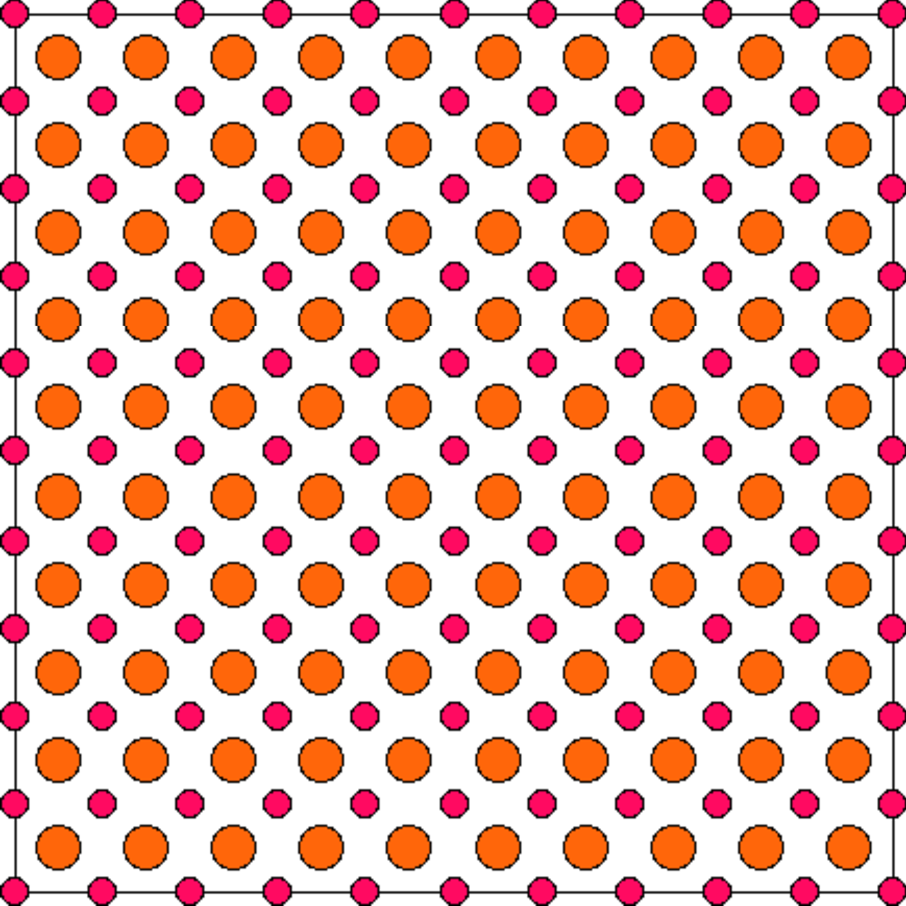
\includegraphics[width=0.30\textwidth]{2_Literature_Review/Fig/GaAs_100.pdf}};
            \draw [fill = black] (0.15, 0.15) rectangle (-0.15, -0.15);
            \draw [white] (0.1, 0.1) -- (-0.1, -0.1);
            \draw [white] (-0.1, 0.1) -- (0.1, -0.1);
        \end{tikzpicture}
    }
    \subcaptionbox{
        \hkl{1 1 0} facet.
        \label{subfig:GaAs_110}
    }{
        \tikzsetnextfilename{GaAs_110}
        \begin{tikzpicture}
            \node[inner sep=0pt] (image) at (0, 0) {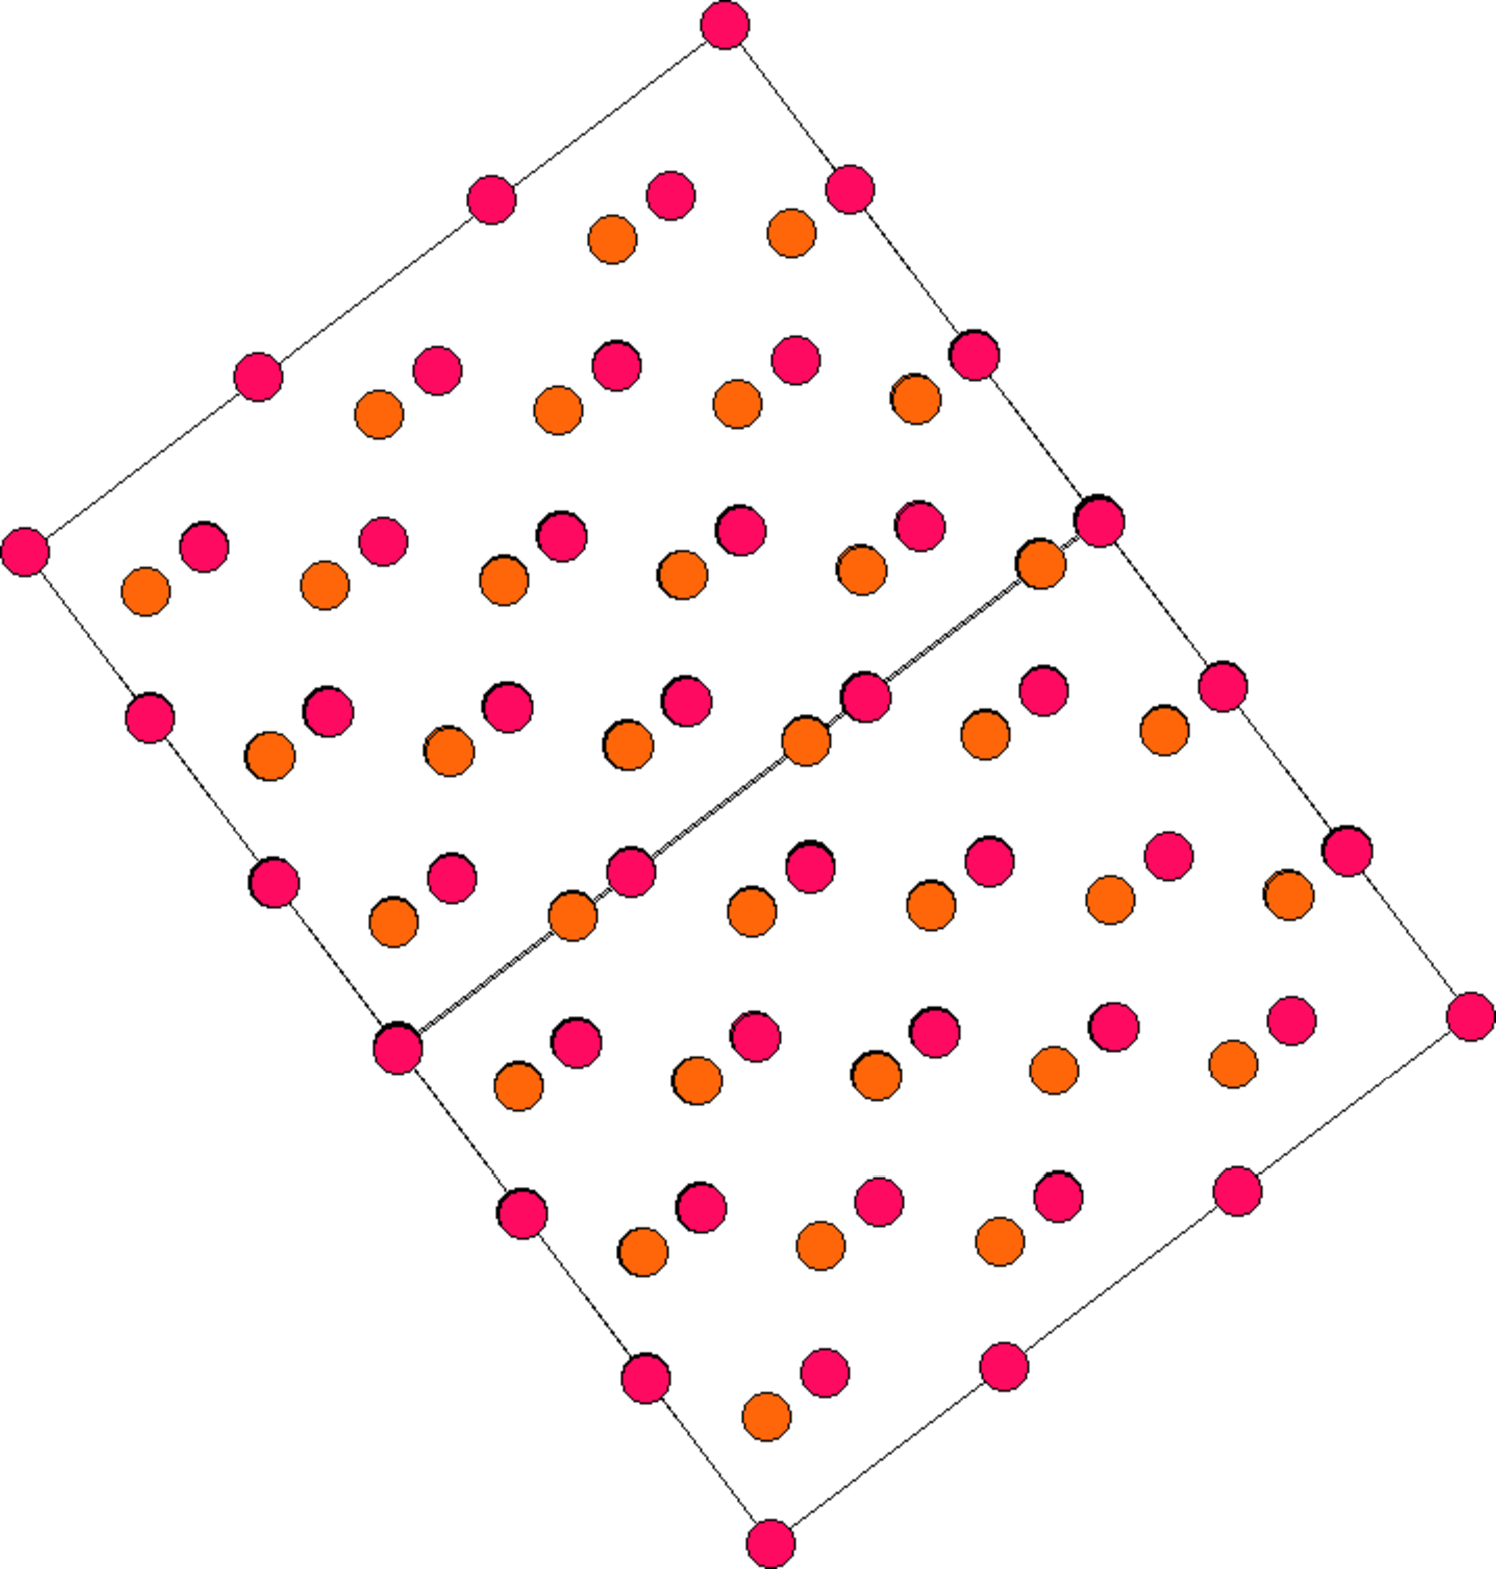
\includegraphics[width=0.30\textwidth]{2_Literature_Review/Fig/GaAs_110.pdf}};
            \begin{scope}[yshift=-0.01]
                \draw (0, 0) -- ++ (37:2);
                \draw (0, 0) -- ++ (37:-2);
                \draw (34:1.9) -- ++ (37:-0.3) -- ++ (-53:0.1) -- cycle;
                \draw (40:1.9) -- ++ (37:-0.3) -- ++ (127:0.1) -- cycle;
            \end{scope}
        \end{tikzpicture}
    }
    \subcaptionbox{
        \hkl{1 1 1}\(_B\) facet.
        \label{subfig:GaAs_111}
    }{
        \tikzsetnextfilename{GaAs_111}
        \begin{tikzpicture}
            \node[inner sep=0pt] (image) at (0, 0) {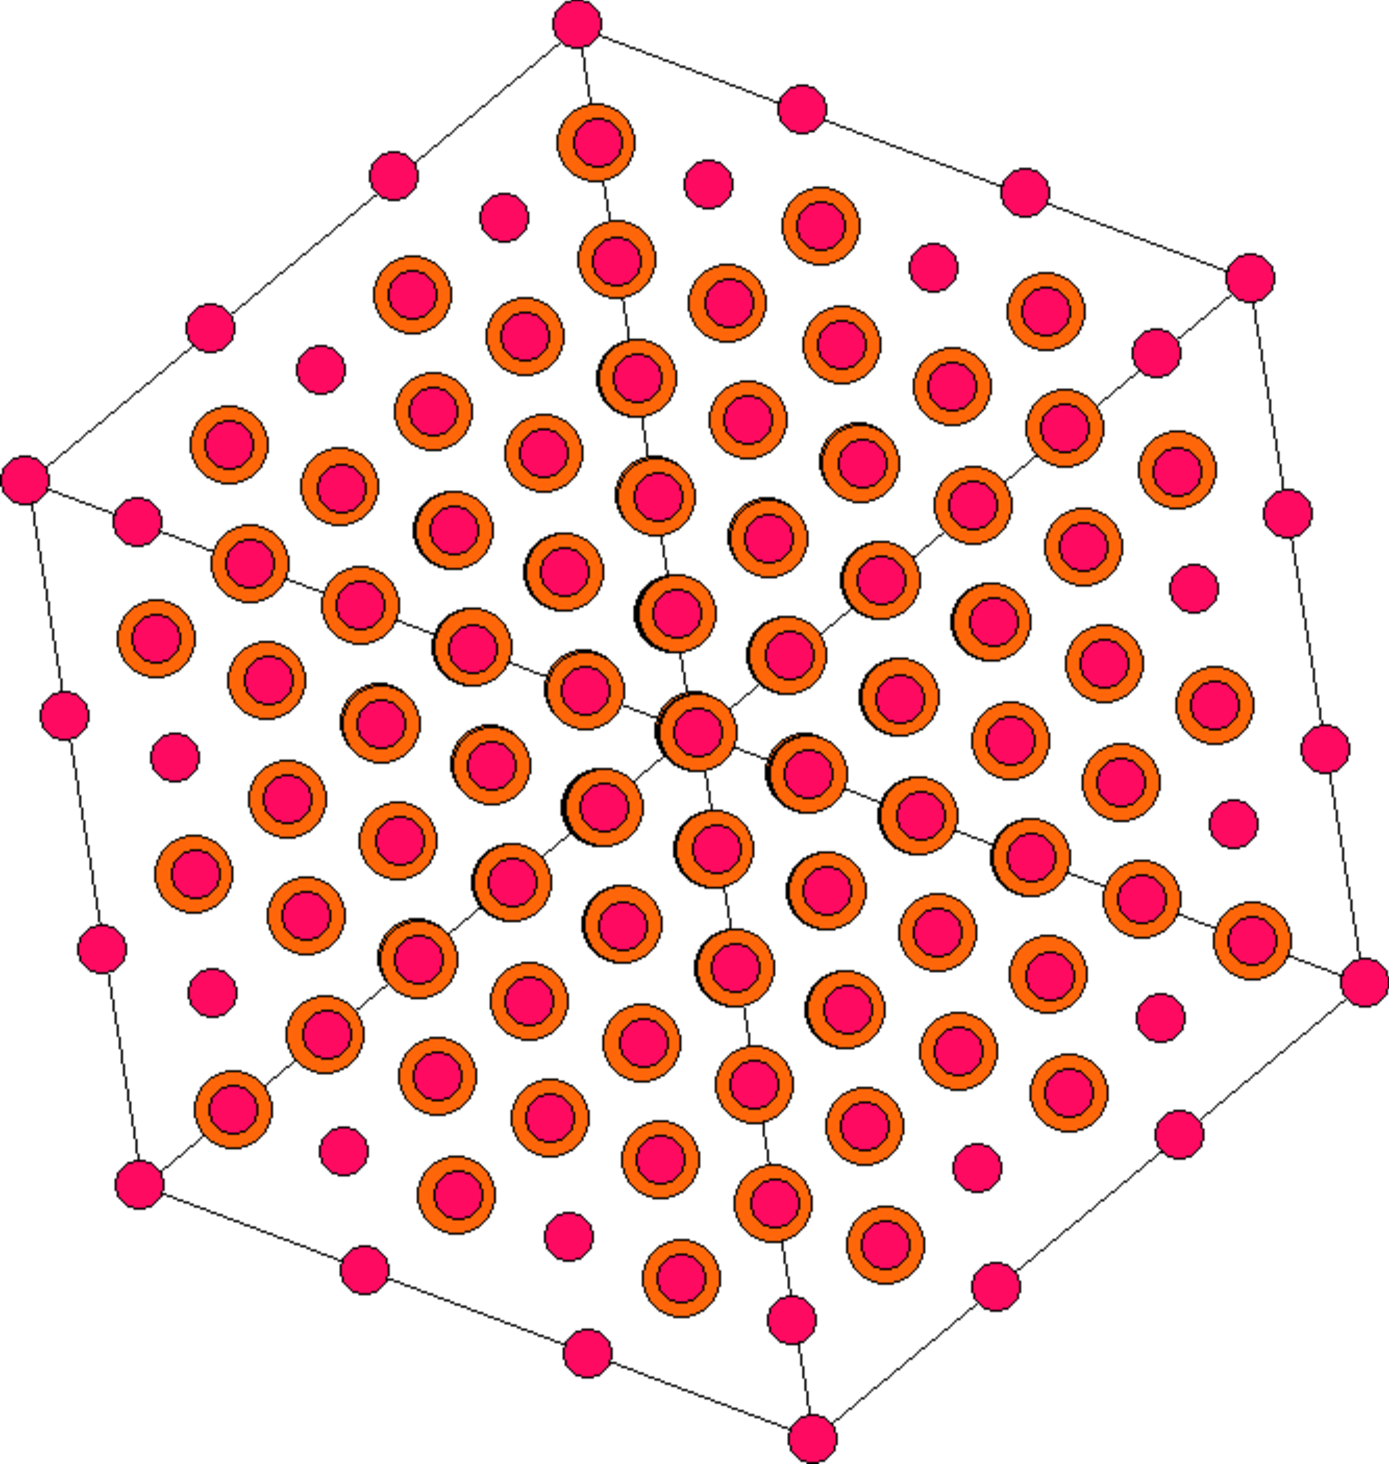
\includegraphics[width=0.30\textwidth]{2_Literature_Review/Fig/GaAs_111.pdf}};
            \draw [fill = black] (0.17, 0) -- ++ (-150:0.3) -- ++ (90:0.3) -- cycle;
            \draw [white] (0, 0) -- ++ (-120:0.1);
            \draw [white] (0, 0) -- ++ (0:0.1);
            \draw [white] (0, 0) -- ++ (120:0.1);
        \end{tikzpicture}
    }
    \caption[Low-index facets in the F\(\bar{4}\)3m \acs{gaas} crystal.]{Simulation of the low-index facets in the F\(\bar{4}\)3m \acs{gaas} crystal with the basic symmetry elements highlighted. \Acl{ga} is represented in orange and \acs{as} in pink; atomic radii are not to scale. \subref{subfig:GaAs_100} shows the 2D projection of the lattice along the \hkl{0 0 1} direction, which coincides with the four-fold axis. \subref{subfig:GaAs_110} shows the 2D projection along the \hkl{1 1 0} direction, contained in the mirror plane. \subref{subfig:GaAs_111} shows the 2D projection along the \hkl{1 1 1} direction, coinciding with the three-fold axis.}
    \label{fig:ZB_low_index_facets}
\end{figure}

III-V semiconductors are compound semiconductors formed by the stoichiometric combination of elements from group III and group V of the periodic table. In their most simple form they are binary, or consisting of one element from group III and one from group V, with some examples being \acs{inp} and \acs{gaas}. Ternary and quaternary III-V materials such as \ce{In1_-_xGa_xAs} or \ce{In1_-_xGa_xAs1_-_yP_y} contain three or four different elements, respectively. 

Crystallographically, III-V materials are available at room temperature in crystals with the symmetries of space group number \num{216} (F\(\bar{4}\)3m, or zincblende-like) or \num{186} (P6\(_3\)mc, or wurtzite-like) and are easily affected by polytypism when grown. Space group \num{216} is that of a cubic face-centred crystal, while space group \num{186} describes a hexagonal crystal. These two structures are closely related, as the addition of a two-fold axis alongside the three-fold axis of space group \num{216} results in a phase change to space group \num{186}, transforming the \hkl<1 1 1> direction in the zincblende phase to the \hkl<0 0 0 1> direction in the wurtzite phase. 

Figure~\ref{fig:ZB_low_index_facets} shows the 2D projections of a \acs{gaas} F\(\bar{4}\)3m crystal along the low-index directions. These projections are useful for the interpretation of atomic-resolution microscopy images of III-V semiconductors. These simulated projections were created using CrystalKit, a dedicated software. They also highlight the main symmetry elements of the zincblende space group. The 2D projection in Figure~\ref{subfig:GaAs_100} shows how a \hkl{0 0 1} facet appears in the microscope. The symmetry element controlling its motif is a four-fold axis perpendicular to the projection plane. Similarly, Figure~\ref{subfig:GaAs_110} shows how a \hkl{1 1 0} facet appears in the microscope and the mirror plane dictating its symmetry. Finally, Figure~\ref{subfig:GaAs_111} shows the lattice projected along the \hkl<1 1 1> direction. The symmetry of this projection is compatible with a three-fold axis coinciding with the \hkl<1 1 1> vector.

\begin{figure}
    \centering
    \subcaptionbox{
        \hkl[0 0 1] corresponding to the z-axis.
        \label{subfig:100_symmetry}
    }{
        \tikzsetnextfilename{100_symmetry}
        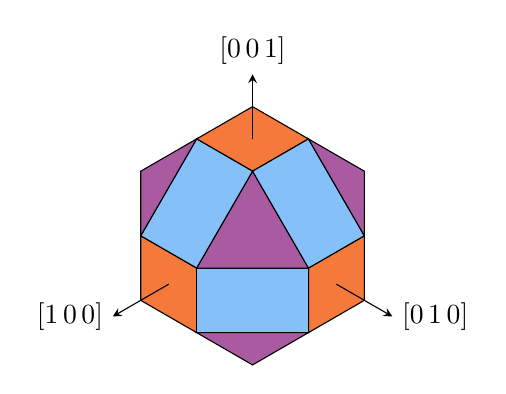
\begin{tikzpicture}[isometric]
            \draw [fill=cb1_orange] (0.5, 0.5, 1.5) -- (-0.5, 0.5, 1.5) -- (-0.5, -0.5, 1.5) -- (0.5, -0.5, 1.5) -- cycle;
            % \draw [fill=red] (0.5, 0.5, -1.5) -- (-0.5, 0.5, -1.5) -- (-0.5, -0.5, -1.5) -- (0.5, -0.5, -1.5) -- cycle;
            \draw [fill=cb1_orange] (1.5, 0.5, 0.5) -- (1.5, -0.5, 0.5) -- (1.5, -0.5, -0.5) -- (1.5, 0.5, -0.5) -- cycle;
            % \draw [fill=green] (-1.5, 0.5, 0.5) -- (-1.5, -0.5, 0.5) -- (-1.5, -0.5, -0.5) -- (-1.5, 0.5, -0.5) -- cycle;
            \draw [fill=cb1_orange] (0.5, 1.5, 0.5) -- (-0.5, 1.5, 0.5) -- (-0.5, 1.5, -0.5) -- (0.5, 1.5, -0.5) -- cycle;
            % \draw [fill=blue] (0.5, -1.5, 0.5) -- (-0.5, -1.5, 0.5) -- (-0.5, -1.5, -0.5) -- (0.5, -1.5, -0.5) -- cycle;
            \draw [fill=cb1_light_blue] (1.5, 0.5, 0.5) -- (1.5, -0.5, 0.5)-- (0.5, -0.5, 1.5) -- (0.5, 0.5, 1.5)  -- cycle;
            \draw [fill=cb1_purple] (0.5, 0.5, 1.5)  -- (1.5, 0.5, 0.5) -- (0.5, 1.5, 0.5) -- cycle;
            \draw [fill=cb1_purple] (0.5, -0.5, 1.5)  -- (1.5, -0.5, 0.5) -- (0.5, -1.5, 0.5) -- cycle;
            \draw [fill=cb1_light_blue] (0.5, 0.5, 1.5) -- (-0.5, 0.5, 1.5) -- (-0.5, 1.5, 0.5) -- (0.5, 1.5, 0.5) -- cycle;
            \draw [fill=cb1_light_blue] (0.5, 1.5, -0.5) -- (0.5, 1.5, 0.5) -- (1.5, 0.5, 0.5) -- (1.5, 0.5, -0.5) -- cycle;
            \draw [fill=cb1_purple] (0.5, 0.5, -1.5) -- (0.5, 1.5, -0.5) -- (1.5, 0.5, -0.5) -- cycle;
            \draw [fill=cb1_purple] (-0.5, 0.5, 1.5) -- (-0.5, 1.5, 0.5) -- (-1.5, 0.5, 0.5) -- cycle;
            \draw [-stealth] (0,0,1.5) -- ++ (0,0,1) node [anchor=east] {\hkl[1 0 0]};
            \draw [-stealth] (0,1.5,0) -- ++ (0,1,0) node [anchor=south] {\hkl[0 0 1]};
            \draw [-stealth] (1.5,0,0) -- ++ (1,0,0) node [anchor=west] {\hkl[0 1 0]};
        \end{tikzpicture}
    }
    \subcaptionbox{
        \hkl[1 1 0] corresponding to the z-axis.
        \label{subfig:110_symmetry}
    }{
        \tikzsetnextfilename{110_symmetry}
        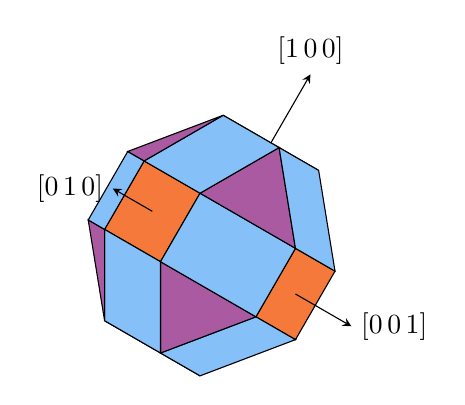
\begin{tikzpicture}[isometric]
            \begin{scope}[rotate around x=45]
                \draw [fill=cb1_orange] (0.5, 0.5, 1.5) -- (-0.5, 0.5, 1.5) -- (-0.5, -0.5, 1.5) -- (0.5, -0.5, 1.5) -- cycle;
                \draw [fill=red] (0.5, 0.5, -1.5) -- (-0.5, 0.5, -1.5) -- (-0.5, -0.5, -1.5) -- (0.5, -0.5, -1.5) -- cycle;
                \draw [fill=cb1_orange] (1.5, 0.5, 0.5) -- (1.5, -0.5, 0.5) -- (1.5, -0.5, -0.5) -- (1.5, 0.5, -0.5) -- cycle;
                % \draw [fill=green] (-1.5, 0.5, 0.5) -- (-1.5, -0.5, 0.5) -- (-1.5, -0.5, -0.5) -- (-1.5, 0.5, -0.5) -- cycle;
                \draw [fill=cb1_orange] (0.5, 1.5, 0.5) -- (-0.5, 1.5, 0.5) -- (-0.5, 1.5, -0.5) -- (0.5, 1.5, -0.5) -- cycle;
                % \draw [fill=blue] (0.5, -1.5, 0.5) -- (-0.5, -1.5, 0.5) -- (-0.5, -1.5, -0.5) -- (0.5, -1.5, -0.5) -- cycle;
                \draw [fill=cb1_light_blue] (1.5, 0.5, 0.5) -- (1.5, -0.5, 0.5) -- (0.5, -0.5, 1.5) -- (0.5, 0.5, 1.5)  -- cycle;
                \draw [fill=cb1_purple] (0.5, 0.5, 1.5)  -- (1.5, 0.5, 0.5) -- (0.5, 1.5, 0.5) -- cycle;
                % \draw [fill=cb1_purple] (0.5, -0.5, 1.5)  -- (1.5, -0.5, 0.5) -- (0.5, -1.5, 0.5) -- cycle;
                \draw [fill=cb1_light_blue] (0.5, 0.5, 1.5) -- (-0.5, 0.5, 1.5) -- (-0.5, 1.5, 0.5) -- (0.5, 1.5, 0.5) -- cycle;
                \draw [fill=cb1_light_blue] (0.5, 1.5, -0.5) -- (0.5, 1.5, 0.5) -- (1.5, 0.5, 0.5) -- (1.5, 0.5, -0.5) -- cycle;
                \draw [fill=cb1_purple] (0.5, 0.5, -1.5) -- (0.5, 1.5, -0.5) -- (1.5, 0.5, -0.5) -- cycle;
                \draw [fill=cb1_purple] (-0.5, 0.5, 1.5) -- (-0.5, 1.5, 0.5) -- (-1.5, 0.5, 0.5) -- cycle;
                \draw [fill=cb1_light_blue] (-0.5, 0.5, -1.5) -- (-0.5, 1.5, -0.5) -- (0.5, 1.5, -0.5) -- (0.5, 0.5, -1.5) -- cycle;
                \draw [fill=cb1_light_blue] (1.5, -0.5, -0.5) -- (1.5, 0.5, -0.5) -- (0.5, 0.5, -1.5) -- (0.5, -0.5, -1.5) -- cycle;
                \draw [fill=cb1_light_blue] (-1.5, 0.5, -0.5) -- (-1.5, 0.5, 0.5) -- (-0.5, 1.5, 0.5) -- (-0.5, 1.5, -0.5) -- cycle;
                \draw [fill=cb1_purple] (-0.5, 0.5, -1.5) -- (-1.5, 0.5, -0.5) -- (-0.5, 1.5, -0.5) -- cycle;
                \draw [-stealth] (0,0,-1.5) -- ++ (0,0,-1) node [anchor=south] {\hkl[1 0 0]};
                \draw [-stealth] (0,1.5,0) -- ++ (0,1,0) node [anchor=east] {\hkl[0 1 0]};
                \draw [-stealth] (1.5,0,0) -- ++ (1,0,0) node [anchor=west] {\hkl[0 0 1]};
            \end{scope}
        \end{tikzpicture}
    }
    \caption[Low index facet orientation in the F\(\bar{4}\)3m space group.]{Low index facet orientation in the F\(\bar{4}\)3m space group. The \hkl{0 0 1}, \hkl{1 1 0}, and \hkl{1 1 1} facets are color-coded in orange, light blue, and purple, respectively. The two orientations shown in this Figure are with the vertical z-axis coinciding with the \hkl[0 0 1] and \hkl[1 1 0] directions in \subref{subfig:100_symmetry} and \subref{subfig:110_symmetry}, respectively.}
    \label{fig:facet_relations}
\end{figure}

Although the orientation of the low index facets with respect to each other is difficult to properly convey on a 2D support, Figure~\ref{fig:facet_relations} shows how the three different facets, \hkl{0 0 1} in orange, \hkl{1 1 0} in light blue, and \hkl{1 1 1} in purple, are orientated in a cubic crystal. The shapes of the polygons that make up the figure also give a hint as to what kind of symmetry element is present in each facet. Figure~\ref{subfig:100_symmetry} can also be used to understand the relationship between different planes in the cubic \acl{si} crystal of the \hkl(0 0 1) \acf{soi} device layer used as seed in Chapter~\ref{chap:growth}. Similarly, Figure~\ref{subfig:110_symmetry} illustrates the symmetry of the \hkl(1 1 0) \acs{soi} device layer used in Chapters~\ref{chap:properties} and \ref{chap:yield_analysis}.

\begin{figure}
    \centering
    \tikzsetnextfilename{GaAs_rtp}
    \begin{tikzpicture}
        \node[inner sep=0pt] (image) at (0, 0) {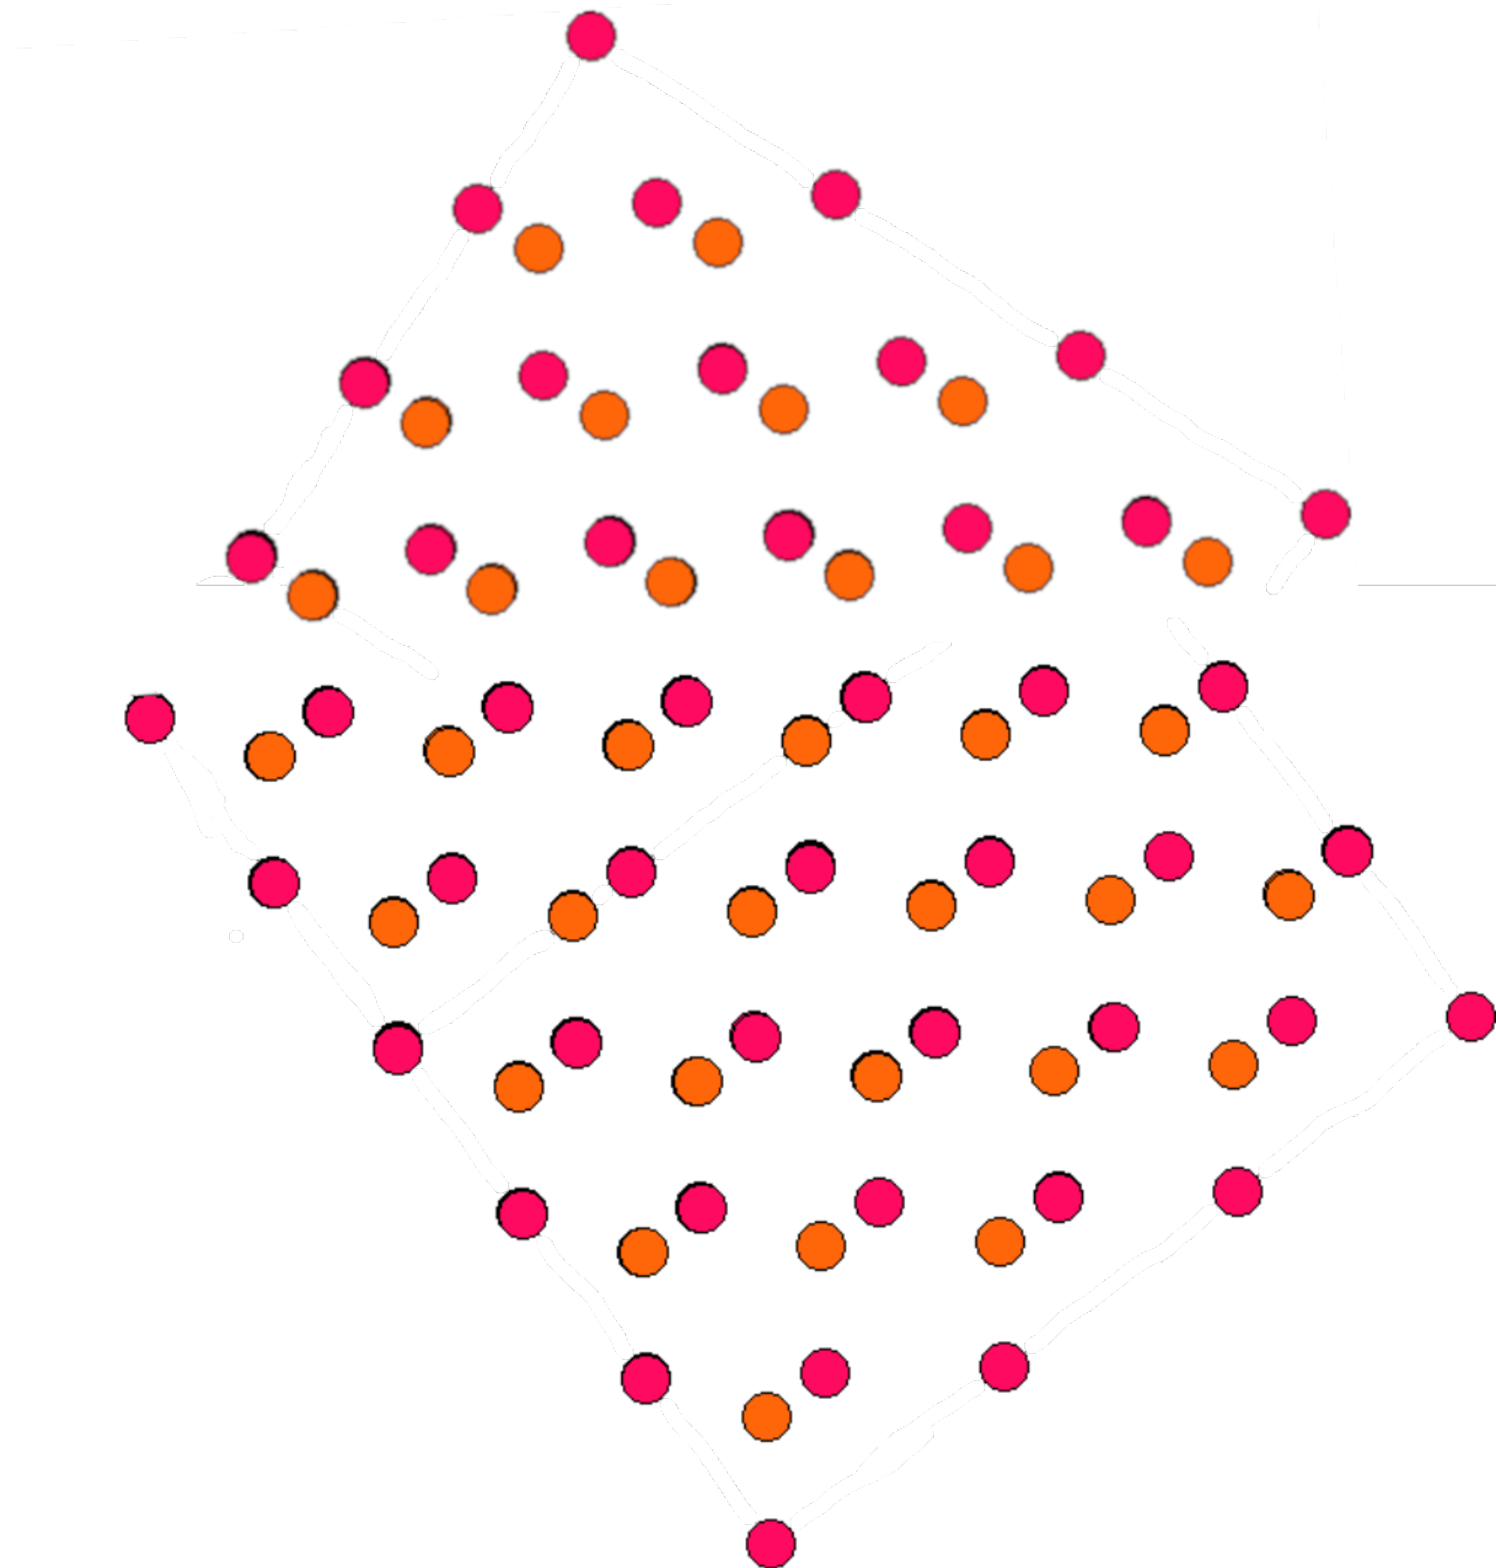
\includegraphics[width=0.3\textwidth]{2_Literature_Review/Fig/GaAs_rtp.pdf}};
        \draw [dashed] (-2.5,0.4) -- ++ (5,0.15) node [anchor = west] {RTP};
    \end{tikzpicture}
    \caption[Drawing of a \hkl{1 1 1} \acl{rtp} in a F\(\bar{4}\)3m crystal.]{Drawing of a \acl{rtp}, highlighted by a dashed line, corresponding to a \hkl{1 1 1} plane in a \acs{gaas} F\(\bar{4}\)3m crystal.}
    \label{fig:GaAs_rtp}
\end{figure}

Figure~\ref{fig:GaAs_rtp} shows a drawing of a \acf{rtp} corresponding to a \hkl{1 1 1} plane in a \acs{gaas} F\(\bar{4}\)3m crystal. Formation of this type of 2D defect is common in the growth of III-V crystals \cite{Borg2017} and its quantity is very sensitive to changes in the growth environment \cite{Algra2008, Chi2013} due to its low formation energy. From a lattice symmetry point of view, the \acs{rtp} is formed by adding a two-fold rotation axis to the \hkl{1 1 1} direction of the crystal. The two atomic bilayers adjacent to the \acs{rtp} can be considered a thin slice of wurtzite \cite{Glas2007, Vedel2022}.

\begin{figure}
    \centering
    \subcaptionbox{
        Band structure of F\(\bar{4}\)3m \acs{inp}.
        \label{subfig:ZB_bands_InP}
    }{
        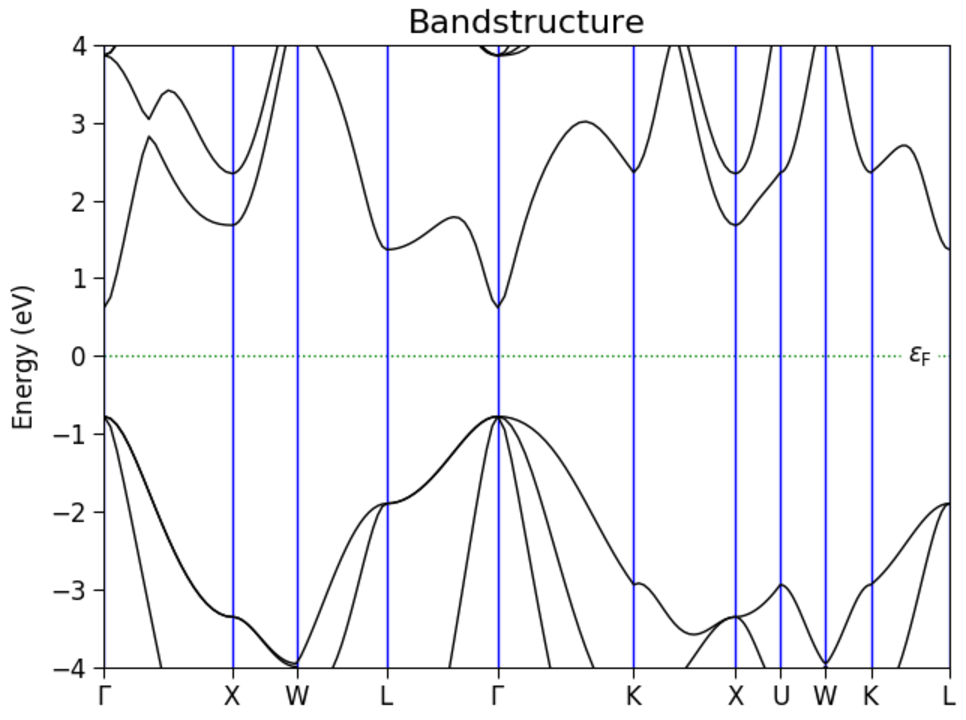
\includegraphics[width=0.48\textwidth]{2_Literature_Review/Fig/Zincblende_bandstructure_InP.pdf}
    }
    \subcaptionbox{
        Band structure of P6\(_3\)mc \acs{inp}.
        \label{subfig:WZ_bands_InP}
    }{
        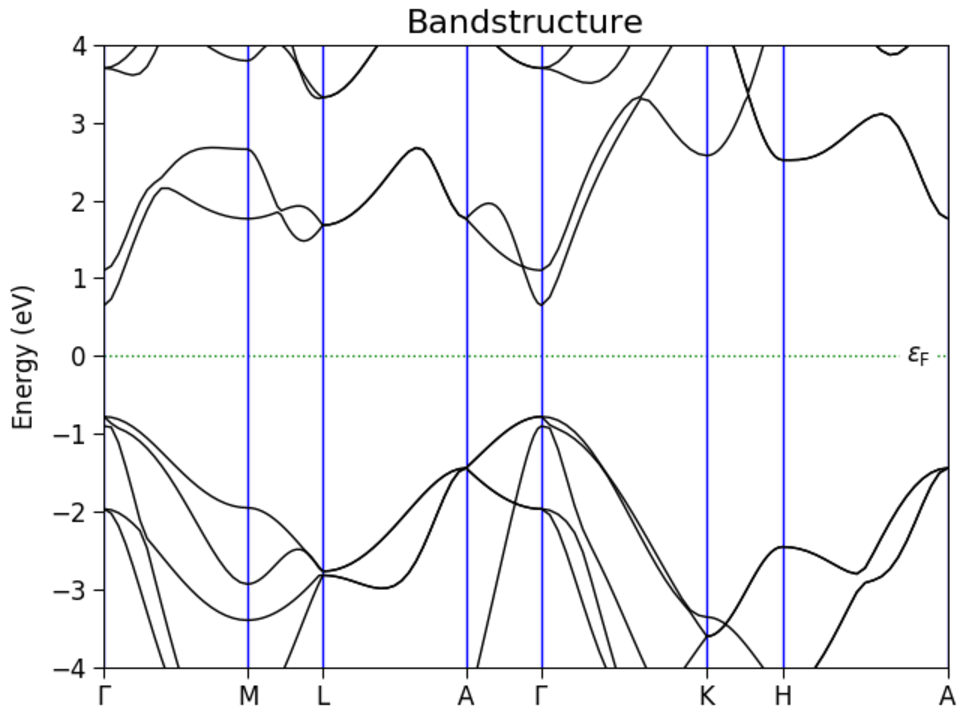
\includegraphics[width=0.48\textwidth]{2_Literature_Review/Fig/Wurtzite_bandstructure_InP.pdf}
    }
    \subcaptionbox{
        Band structure of Fd\(\bar{3}\)m \acs{si}.
        \label{subfig:Si_bands}
    }{
        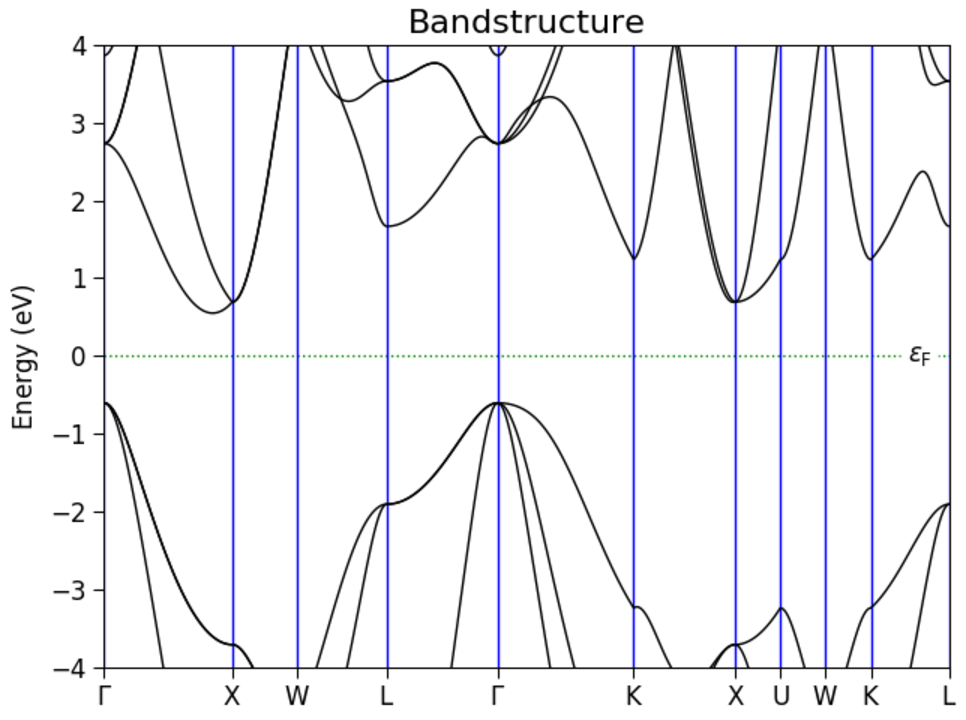
\includegraphics[width=0.48\textwidth]{2_Literature_Review/Fig/Silicon_bandstructure.pdf}
    }
    \caption[Band structures of \acl{si}, and \acs{inp} in its cubic and hexagonal phases.]{Band structures of \acl{si}, and \acs{inp} in its cubic and hexagonal phases, calculated with \acs{dft}. \subref{subfig:ZB_bands_InP} and \subref{subfig:WZ_bands_InP} show the band structures of zincblende and wurtzite \acs{inp}. \subref{subfig:Si_bands} shows the band structure of Fd\(\bar{3}\)m \acs{si}.}
    \label{fig:band_structure}
\end{figure}

Both atomic species and lattice symmetry affect the electronic properties of crystals. 













\section{\texorpdfstring{III-V-on-\acs{si} integration routes}{III-V-on-Si integration routes}}
The various integration routes of III-V semiconductors on Si can be divided in two broad categories: heterogeneous and homogeneous integration.

CHANGE TO TRANSFER AND MONOLITHIC GROWTH

\subsection{Heterogeneous integration}
Heterogeneous integration refers to the indirect integration of III-V material grown on a different, lattice matched, substrate on a Si wafer. 
\par
The main advantage of these techniques is the elimination of lattice mismatch as a source of defects during epitaxial growth. Furthermore, it allows the selection of the best-performing structures to be transferred onto the Si substrate \cite{Zadeh2016, Wang2017}, and does not have to compromise on the growth parameters or material systems for the sake of CMOS compatibility (except for bonding temperature). The various methods that fall under this definition form, all together, a mature technology that already finds application in industry4, therefore benefitting from a few years of industrial optimisation.
\par
On the other hand, this type of integration requires the growth of III-V to take place in a different fabrication line that must maintain the high precision and cleanliness standard of the main CMOS silicon line, resulting in a rather large capital investment. Furthermore, most classic transfer steps can result in a material with a more irregular geometry (wafer bow, surface roughness after etching), or presenting transfer-related defects \cite{Jevtics2022}, or require an extra bonding layer \cite{Jevtics2022, Tang2019}, and do not allow for nm precise integration \cite{Wang2017, McPhillimy2020}. However, the most advanced techniques that bypass most of these quality issues are too slow to provide a competitive transfer time for large, densely integrated 8' production wafers \cite{Wang2017, McPhillimy2020}.
\subsection{Homogeneous Integration}
Homogeneous integration refers to the direct integration by epitaxial growth of III-V semiconductors on Si. 
It naturally provides advantages such as the extremely high spatial precision and accuracy for the integration of small devices on wafer-scale substrates, which can be achieved in a shorter time frame compared to its heterogeneous analogues \cite{Wang2017}. It has the potential of being a more economical alternative to heterogeneous integration. If the growth process can be integrated with current CMOS processes, its implementation in a CMOS line would render having an entire dedicated III-V fab running in parallel with a Si-based fab unnecessary, especially if the use of III-V electronics is envisioned at the same time as III-V photonics \cite{Wang2017}, therefore potentially reducing the capital cost required to implement this efficient light-emitting and -absorbing material in different devices \cite{Tang2019}.
The main disadvantage is related to the high lattice mismatch between Si and most III-V materials, meaning strain-relaxing defects are nucleated at the heterointerface \cite{Kunert2018}: these defects have a very detrimental effect on the performance and lifetime of devices \cite{Mahajan2000, Zenari2021}, and act as scattering or recombination centres \cite{Jeon2015}. The polar nature of III-V atomic bonds compared to nonpolar Si-Si bonds can create anti-phase boundaries during growth on certain Si facets \cite{Kunert2018}, and most known surface treatments to eliminate the nucleation sites for these defects occur in temperature ranges that are incompatible with the CMOS process \cite{Miller2000}. Furthermore, materials that are known to grow at a higher temperature, such as III – nitrides, and others that could have detrimental effects on the passivating of SiO2 layers, such as gallium \cite{Miller2000}, also pose compatibility problems with the CMOS process. Another key obstacle, especially related to the direct growth of micro- and nanostructures, is the stricter requirements for the reproducibility and reliability of the process.
\subsection{Comparison between homogeneous integration routes}
What follows is a table comparing the advantages and disadvantages of various homogeneous integration techniques. The table predominantly focusses on what can be accomplished in the growth reactor and briefly mentions techniques that require simple or complex substrate preparation.


\begin{sidewaystable}
    \centering
\begin{longtable}{p{0.1\textwidth}|p{0.42\textwidth}|p{0.42\textwidth}}
    Type & Advantages & Disadvantages \\ \hline \hline
    Planar growth & 
    \begin{itemize}
        \item Extremely simple substrate preparation steps.
        \item Allows Stranski-Krastanov growth mode for quantum dot formation \cite{Shi2016, Reithmaier2016}
    \end{itemize} & 
    \begin{itemize}
        \item Often leads to wafer bow or warp due to thermal expansion coefficient mismatch \cite{Miyoshi2016, Wang2017_2}
        \item Can require 1+ micrometre thick strain management layer before device growth (depending on mismatch) \cite{Wang2017_2, Cantoro2012}
        \item Widespread defects are common in this kind of growth \cite{Ravash2012}
    \end{itemize} \\ \hline
    Selective Area Growth (SAG) & 
    \begin{itemize}
        \item Substrate preparation ranges from relatively simple to somewhat complex
        \item Allows the growth of nanostructures \cite{Cantoro2012}
        \item Allows the growth of core-shell wires \cite{Tomioka2011}
        \item Allows position control \cite{Tomioka2011}
        \item No wafer warp or bow as a result of the III-V material
        \item Allows the growth of various device structures, but only vertically \cite{Bi2019, Staudinger2021}
    \end{itemize}  & 
    \begin{itemize}
        \item Sidewall growth can be minimized but not eliminated, resulting in undesired heterointerfaces and possible loss of composition control in complex systems.
        \item Growth mainly happens in the vertical direction
    \end{itemize}  \\ \hline
    VLS/Droplet epitaxy (vertical nanowires) & 
    \begin{itemize}
        \item Simple substrate preparation process
        \item Allows for nanostructure growth \cite{Wagner1964}
        \item No wafer warp or bow as a result of the III-V material
        \item Allows for sophisticated growth studies such as in-situ TEM imaging \cite{Maliakkal2020, Jacobsson2016, Harmand2018}, leading to the possibility to refine growth recipes to the point where phase control can be achieved \cite{Algra2008, Caroff2009, Joyce2007}.
        \item Can be tuned to achieve high directionality of the growth and possibility to incorporate heterostructures with minimal or no undesired side growth \cite{Harmand2018, Joyce2007}
    \end{itemize}  & \begin{itemize}
        \item Limited position control \cite{Joyce2007}
        \item Nanostructure geometry limited to nanowires \cite{Wagner1964}
        \item Reservoir effect complicates composition control in ternary and quaternary compounds \cite{Dubrovskii2017}
    \end{itemize} \\ \hline
    \caption{Caption}
    \label{tab:methods1}
\end{longtable}
\end{sidewaystable}
    \begin{sidewaystable}
    \centering
    \begin{longtable}{p{0.1\textwidth}|p{0.42\textwidth}|p{0.42\textwidth}}
    Type & Advantages & Disadvantages \\ \hline \hline
    Selective Area Growth with Aspect Ratio Trapping & 
    \begin{itemize}
        \item Allows position control for the III-V growth29
        \item Highly reduced bow and warp effect on the wafer after deposition
        \item Aspect ratio trapping (ART) allows a base level of defect control \cite{Han2016}
    \end{itemize}  & \begin{itemize}
        \item Defects propagating in any direction that shares the plane of the side walls are not filtered2
        \item Multiple nucleation points can result in grain boundaries, and their elimination requires extra process steps \cite{Kunert2016}
    \end{itemize} \\ \hline
    Template Assisted Selective Epitaxy (TASE) & 
    \begin{itemize}
        \item Allows the growth of a very large variety of both vertical and horizontal nanostructures while maintaining extremely accurate geometry and  position control \cite{Ritter2021, Tiwari2020, Schmid2015}
        \item Superior defect control, even compared with ART: far from the growth interface defects can be effectively limited to twin planes \cite{Han2020}, which in some cases can too be eliminated \cite{Knoedler2017}
        \item Potential for excellent facet and composition \cite{Borg2019, Goswami2020} control in nanowires, with no side growth when growing heterostructures \cite{Brunelli2019} 
        \item No wafer warp or bow as a result of the III-V material
        \item Allows for phase control in determinate growth geometries \cite{Staudinger2018}
    \end{itemize} & 
    \begin{itemize}
        \item Substrate preparation takes place in a complex multi-step process
        \item Can suffer from parasitic growth
        \item Some height limitations in terms of core shell structures, which can’t be grown horizontally, and are de-facto limited to microdisk form factors \cite{Tiwari2020}
    \end{itemize} \\ \hline
    \caption{Caption}
    \label{tab:methods2}
\end{longtable}
\end{sidewaystable}

It should be noted that often, in papers from Dr. Lau’s group, the growth method they use is called lateral aspect ratio trapping (LART) \cite{Han2020, Yan2021}: this is in essence a hybrid between SAG-ART and TASE, and can be described as a type of TASE with particularly wide (sometimes several micrometres) templates, therefore I have grouped it with TASE in the above table. It should be noted, however, that while LART offers most of the same advantages that TASE offers, it is more susceptible to the formation of grain boundaries due to multiple nucleation (which does not take place in TASE) and has reduced defect trapping in the wide direction. On the other hand, due to their etch-based approach, they can achieve more intricate quantum well positioning in their microdisk lasers than what is possible with our TASE approach for microdisk growth.



111B growth outside of tase

\section{\texorpdfstring{State of \acl{tase}}{State of template assisted selective epitaxy}}
\section{Characterization of nano- and microstructures}
Talk about defect types (what is an rtp is very important) and therefore about the lattices

TALK ABOUT IMPORTANCE OF SINGLE FACET FOR INCORPORATION RATES (SEE FOLLOWING SECTION)

\section{Article 2}

Due to the presence of the SiO2 template, the quantum wells
develop only axially and not laterally. This results in improved
composition control in heterolayers of ternary III-V
compounds incorporated in the nanowires\cite{Borg2019} and therefore is
expected to allow for better control of the emission spectra.
%\chapter{III-V growth in TASE samples}
\label{chap:growth}

For over a decade, research on monolithic integration of III-V semiconductors has been conducted at \acs{ibm} Research Europe - Zurich. The \acf{tase} method was thought of and developed during this long research effort \cite{borgTASEp2018, Mauthe2021}. \acs{tase} was then applied to integrate emitting and absorbing electronic elements, such as lasing microdisks and nanowire-based photodetectors. As I joined \acs{ibm}, research on both of these device architectures was still ongoing, and, as I was familiarising myself with the tools necessary to conduct my research in the first months of my PhD, I had the opportunity to cooperate with other team members on their projects \cite{Tiwari2021}. Dr. Wen led one such project and aimed to create a single nanowire photodetector. In the end, the project achieved its goal, as seen in \cite{Wen2022}. However, one particular aspect that still needed improvement if the single sample shown in the paper was to be reproducible was the control of the growth front morphology.

Controlling the morphology of the growth front is essential for several reasons. The first is that by ensuring a specific shape of the various heterolayers, the metal-to-semiconductor contact regions can be determined more accurately, aiding in further process steps. The second reason contends with the different integration rates of III elements on different facets. This was already explored by previous team members, who showed a marked dependence of the atomic fraction of the III element in \acs{ingaas} from the facet on which it was grown \cite{Borg2019}.

\begin{figure}
    \centering
    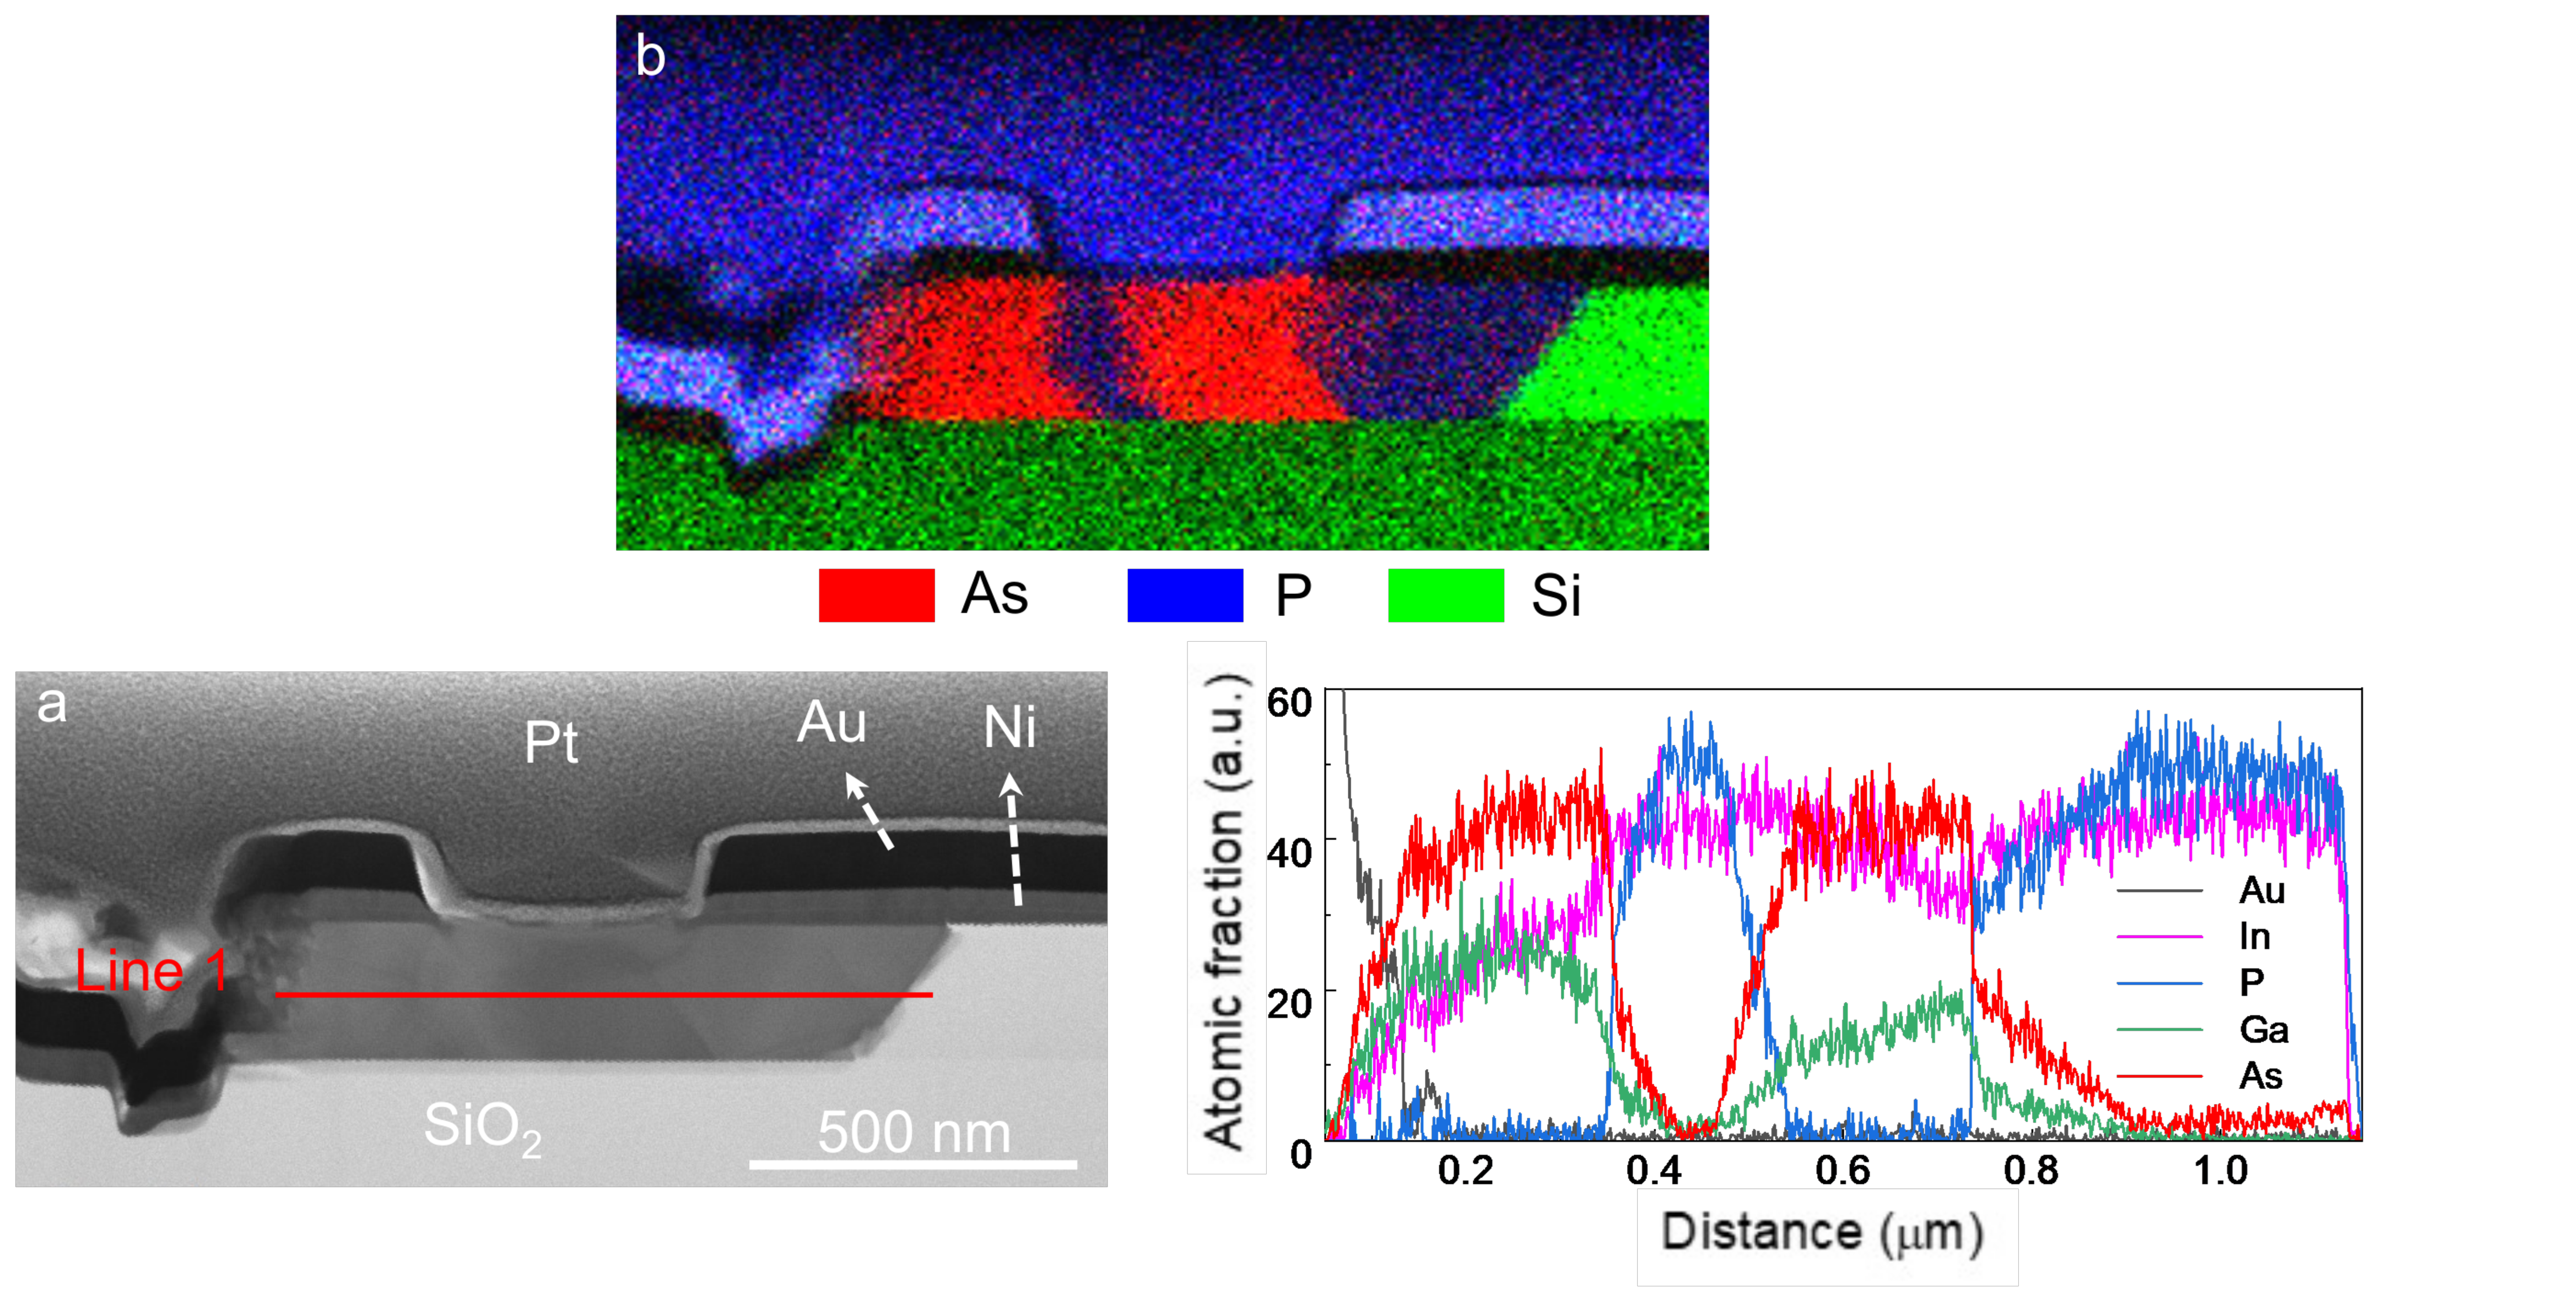
\includegraphics[width = \textwidth]{3_Growth/wen.pdf}
    \caption{Structural and compositional analysis of a nanowire detector carried out by Wen \textit{et al.} Adapted from \cite{Wen2022} licensed under CC BY 4.0 \cite{CCBY40}.}
    \label{fig:wen}
\end{figure}

Figure~\ref{fig:wen} shows the structure and composition of the nanowire characterised by Wen \textit{et al.} in \cite{Wen2022}. The \acs{bf}-\acs{stem_m} image in Figure~\ref{fig:wen}(a) shows the morphology of the nanowire. A \hkl{1 1 1} \acs{si} facet on the right of the image served as the nucleation surface from which the heterostructures nanowire grew. The nickel-gold contacts are placed at the two \textit{p} and \textit{n} ends of the doped III-V \textit{p}-\textit{i}-\textit{n} diode. The \acf{eds} map in Figure~\ref{fig:wen}(b) reveals how to obtain the performance described in their article. The authors precisely deposited the metal contact to cover the exact regions of \textit{p} doped \acs{ingaas} at the end of the wire and \textit{n} doped \acs{inp} closer to the seed. The authors report a good performance for the final device. Despite this, they note some reproducibility issues in the discussion section of their paper, namely regarding contact placement. This is because the growth front geometry in \acs{tase} has been shown to depend on specific parameters but to be essentially stochastic when, as with the sample in Figure~\ref{fig:wen}, there is a multifaceted growth front. This, in turn, means that material layers that should have the same thickness can vary in shape and, therefore, have a different contactable area at their top interface, changing the distance between contacts wire-by-wire and complicating direct performance comparisons between different devices. Finally, the graph in Figure~\ref{fig:wen} shows the sample's composition profile, highlighting its broad composition gradients. These are highly dependent on the shape of the various heterointerfaces and, therefore, the growth front. It is then clear that achieving a single-facet, reproducible growth front is the key to improving the reproducibility of devices grown with \acs{tase}.

This chapter expands on the research published by my co-authors and me in \cite{Brugnolotto2023}. I will first talk about the most common crystalline defects that can be observed in \acs{stem_m} images of \acs{tase} grown structures, to complement the compositional and morphological discussion in the introduction of this chapter. An in-depth exposition of the nanowire design and growth recipes, and their analysis follows, explaining the evolution of the methodology from a simple thick bi-layer heterostructure to a multi-\acl{qw} architecture with single facet heterointerfaces. When discussing the order of appearance of the wire's internal structured in this thesis, the 0 point is always found at the \acs{si} seed interface, regardless of its position in the image.

\section{Initial measurements on pre-existing samples}
As the previous section shows, \acs{tase} has been developing for the last decade \cite{Borg2014}. As such, when I started working on the project, an initial study was conducted to determine the crystalline quality of \acs{tase}-grown structures from other ongoing projects. 

\subsection{\texorpdfstring{Defects in \acs{tase} samples}{Defects in TASE samples}}
\label{subsec:pre-existing_samples}

\begin{figure}
    \centering
    \subcaptionbox{Cross section of a multi-seeded coalesced III-V structure grown on Si.
        \label{subfig:SM_overview}
        }{
        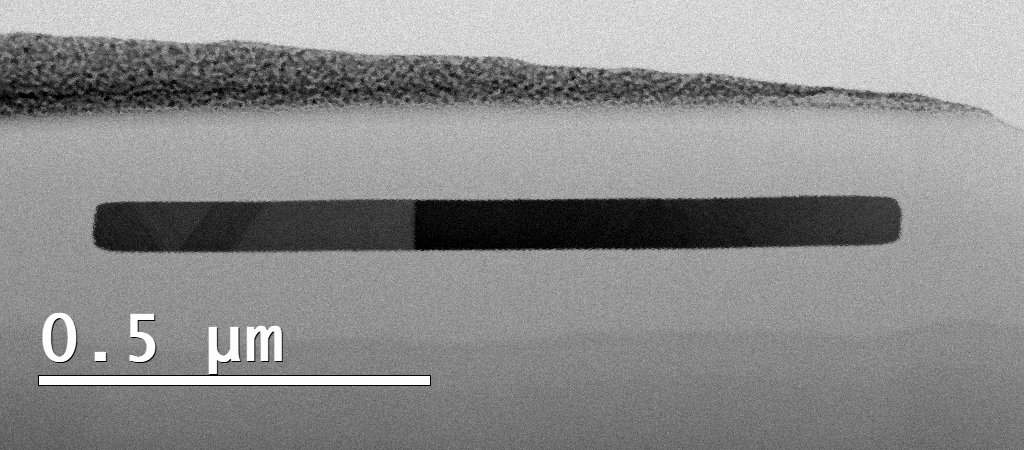
\includegraphics[width = 0.98\textwidth]{3_Growth/2020_Merge/JEOL_BF_150k_SOU76posB_Tunnel5Overview.png
        }
    }
    \subcaptionbox{Detail of twin planes and dislocations.
        \label{subfig:SM_dislocations}
        }{
        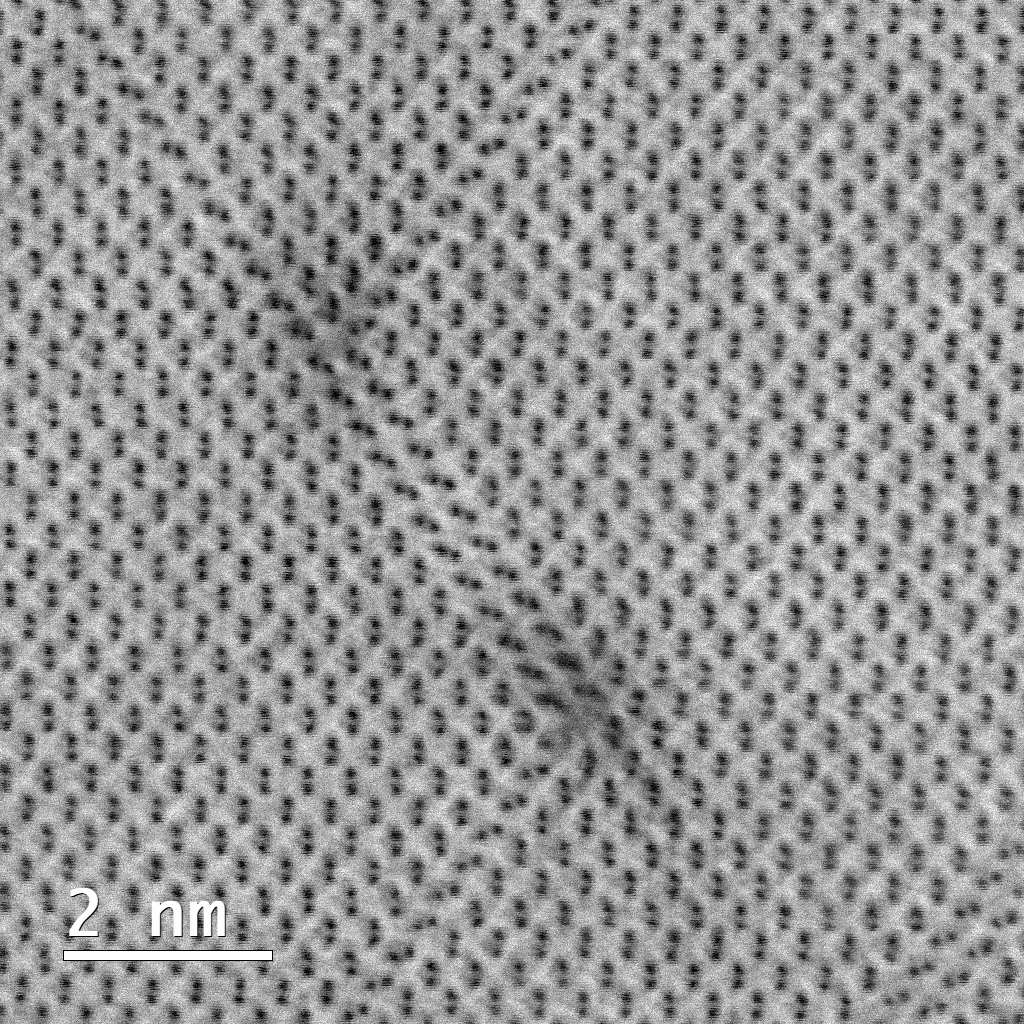
\includegraphics[width = 0.48\textwidth]{3_Growth/2020_Merge/JEOL_BF_20M_SOU76posB_Tunnel5Seed1DefectMeet1.png
        }
    }
    \subcaptionbox{Detail of a grain boundary.
        \label{subfig:SM_merge_position}
        }{
        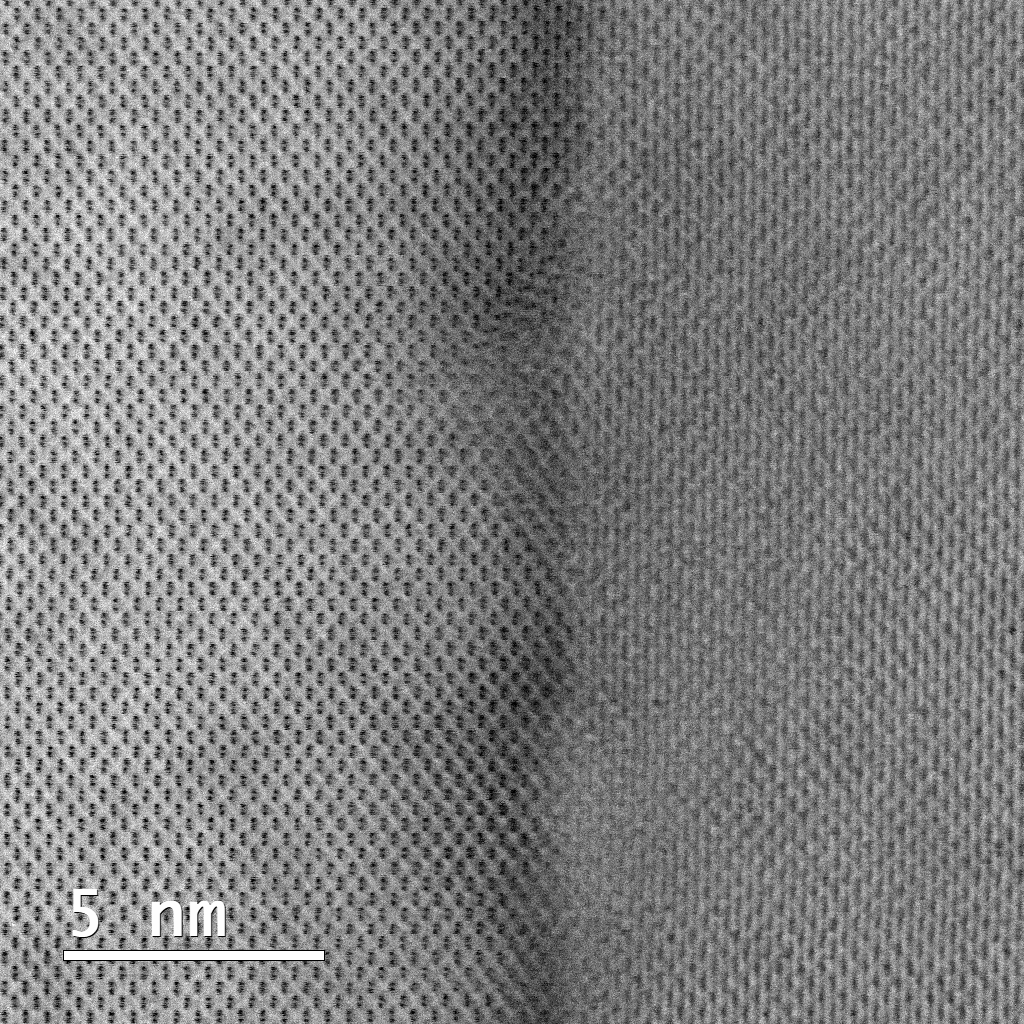
\includegraphics[width = 0.48\textwidth]{3_Growth/2020_Merge/JEOL_BF_10_M_SOU76posB_Tunnel5_Boundary_Seeds_2_3.png
        }
    }
    \caption{\acs{bf}-\acs{stem_m} images of a cross section of a \acs{tase} structure. \subref{subfig:SM_overview} overview image of the entire platelet. Two regions can be identified in this image, with the leftmost area of the left section presenting an area with darker lines describing a "v" shape. These lines are caused by \acs{rtp}s. \subref{subfig:SM_dislocations} a pair of stair-rod dislocations \cite{Bologna2018} imaged in high-resolution. \subref{subfig:SM_merge_position} high-resolution image of the area in which the two regions in \subref{subfig:SM_overview} meet.}
    \label{fig:2020_Merge}
\end{figure}

From the measurement conducted on various \acs{tase}-grown samples, it was apparent that the most common crystalline defect was the twin plane, with a widespread presence of micro twins in all the samples analysed. Only one of the structures, created by merging different nanowires into a larger platelet, had dislocations (Figure~\ref{subfig:SM_dislocations}). 
\par
The sample in Figure~\ref{fig:2020_Merge} was grown by Svenja Mauthe before the beginning of my stay at \acs{ibm} Research Europe - Zurich as part of her study on the controlled introduction of dislocation at the merging point of two growing crystals \cite{Mauthe2021}. A cross-section of a structure deriving from one such experiment is shown in Figure~\ref{subfig:SM_overview}. This lamella was cut in the area of the device where the wires had already merged. Two areas of the structure stand out particularly: on the left side of the image, a series of "v-shaped" parallel lines denote the presence of two-fold \acf{rtp}s in orthogonal \hkl{111} planes. In this region, Figure~\ref{subfig:SM_dislocations} shows the two stair-rod dislocations forming where two twin planes intersect or when one is annihilated and the other changes direction. This type of defect was the subject of an in-depth study by Bologna et al. \cite{Bologna2018}, but it will not make another appearance in any of the other \acf{stem_m} images recorded during my studies. However, it should be noted that the vast majority of cross sections imaged from this point on were cut along the growth axis instead of perpendicularly to it as this one was. Figure~\ref{subfig:SM_merge_position} shows the interface between the light grey and dark grey segments that comprise the III-V crystal in Figure~\ref{subfig:SM_overview}. 
\par
As made clear by the definition with which the atomic columns are visible on the left-hand side of Figure~\ref{subfig:SM_merge_position} the sample was orientated to achieve the channelling condition of the \acs{stem_m} electron beam in the corresponding crystal. The crystal's lattice on the right-hand side of the same image does not appear as clearly defined: a slight rotation at the time of nucleation might have happened for one of the two seeds pictured. Of course, since the platelet originated from five different seeds, an empirical assumption can be made about two of them prevailing over the other three. This hypothesis is further supported by the presence of \acs{rtp}s on the leftmost portion of the crystalline slice in Figure~\ref{subfig:SM_overview}. At the same time, the area to its immediate right does not show signs of \acs{rtp}s, hinting at the possibility of growth developing in two different directions. 

\section{\texorpdfstring{Fabrication on \acs{si}\hkl(0 0 1) \acs{soi}}{Fabrication on Si(001) SOI}}
Nanofabrication was carried out with the \acs{tase} process (see \autoref{chap:tase} for details) and, together with the later sample characterisation, took place in highly controlled environments such as a cleanroom and noise-free lab (see \autoref{chap:tools}). Firstly, the shape of the ensemble of nucleation seed and nanostructure is transferred to the \acs{si} device layer of the \acs{soi} wafer through a series of lithographic and etching steps. The template, composed of \acs{sio2}, is then deposited on top of the resulting microstructures. Finally, the template is opened in one or more positions before the etch-back of the sacrificial \acs{si} volume and the introduction of \acf{mocvd} grown III-V semiconductor in its place \cite{Schmid2015, borgTASEp2018}.
\par
Initial growth experiments focussed on nanowires, one of the simplest geometries. The relative simplicity of the nanowires allows for the study of the impact of even minor modifications of the growth recipes on the final crystal, both in terms of structure and composition.

\subsection{Template design considerations}

\begin{figure}
    \centering
    \subcaptionbox{
    \hkl(0 0 1) in-plane crystalline directions.
    \label{subfig:001wafer_directions}
    }{
        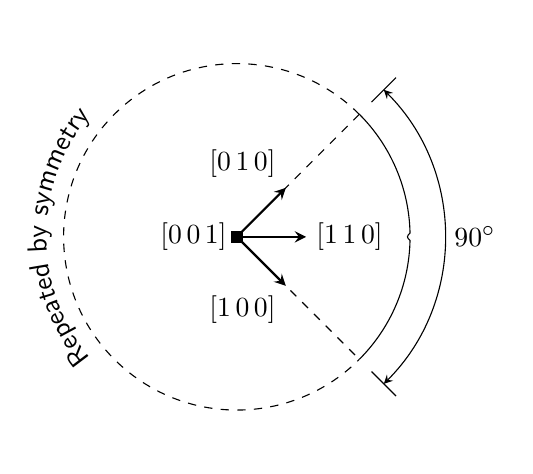
\begin{tikzpicture}
            \begin{scope}[scale=0.22]
                \draw (45:11cm) -- (45:13cm);
                \draw[stealth-stealth] (45:12cm) arc [start angle = 45, end angle = -45, radius = 12cm] node[midway, anchor = west]{\qty{90}{\degree}};
                \draw (-45:11cm) -- (-45:13cm);
                \draw (-45:10cm) arc [start angle=315, end angle=358.8, radius=10cm] -- (9.8935cm,-1.065mm) arc [start angle=-135, end angle=-225, radius=1.5mm] -- (9.9987cm,2.13mm) arc [start angle=1.20, end angle=45, radius=10cm];
                \draw[dashed] (45:10cm) arc [start angle=45, end angle=315, radius=10cm];
                \path[decorate,decoration={text along path, text={Repeated by symmetry},text align=center}] (315:11) arc [start angle=315,end angle=45,radius=11];
                \draw[dashed] (45:10cm) -- (0, 0) -- (-45:10cm);
                \draw[-stealth, thick] (0, 0) node[anchor=east] {\hkl[0 0 1]} -- ++ (0:4cm) node[anchor=west] {\hkl[1 1 0]};
                \draw[-stealth, thick] (0, 0) -- ++ (45:4cm) node[anchor=south east] {\hkl[0 1 0]};
                \draw[-stealth, thick] (0, 0) -- ++ (315:4cm) node[anchor=north east] {\hkl[1 0 0]};
                \node[mark size=2pt] at (0, 0) {\pgfuseplotmark{square*}};
            \end{scope}
        \end{tikzpicture}
    }
    \subcaptionbox{
    Microstructure designs.
    \label{subfig:enterprise_design}
    }{
        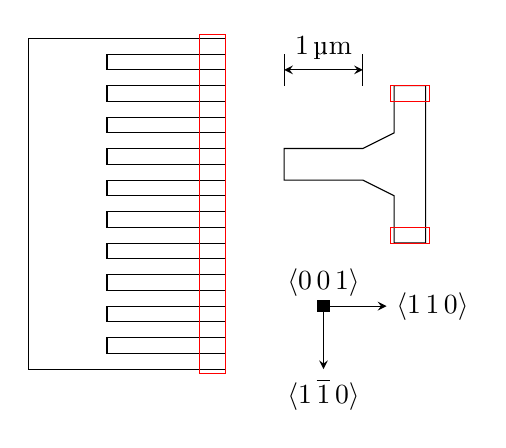
\begin{tikzpicture}
            \begin{scope}[scale=0.1]
                \draw (20, 1) -- ++ (10, 0) -- ++ (-26.6:4.445) -- ++ (0, -6) -- ++ (4, 0) -- ++ (0, 20) -- ++ (-4, 0) -- ++ (0, -6) -- ++ (26.6:-4.445) -- ++ (-10, 0) -- cycle;
                \draw[red] (33.5, 11) rectangle (38.5, 13);
                \draw[red] (33.5, -7) rectangle (38.5, -5);
                \draw (-12.5, -23) -- ++ (25, 0) -- ++ (0,2) -- ++ (-15, 0) -- ++ (0, 2) -- ++ (15, 0) -- ++ (0,2) -- ++ (-15, 0) -- ++ (0, 2) -- ++ (15, 0) -- ++ (0,2) -- ++ (-15, 0) -- ++ (0, 2) -- ++ (15, 0) -- ++ (0,2) -- ++ (-15, 0) -- ++ (0, 2) -- ++ (15, 0) -- ++ (0,2) -- ++ (-15, 0) -- ++ (0, 2) -- ++ (15, 0) -- ++ (0,2) -- ++ (-15, 0) -- ++ (0, 2) -- ++ (15, 0) -- ++ (0,2) -- ++ (-15, 0) -- ++ (0, 2) -- ++ (15, 0) -- ++ (0,2) -- ++ (-15, 0) -- ++ (0, 2) -- ++ (15, 0) -- ++ (0,2) -- ++ (-15, 0) -- ++ (0, 2) -- ++ (15, 0) -- ++ (0,2) -- ++ (-15, 0) -- ++ (0, 2) -- ++ (15, 0) -- ++ (0,2) -- ++ (-25, 0) -- cycle;
                \draw[red] (9.2, -23.5) rectangle (12.5, 19.5);
                \draw[stealth-stealth] (20, 15) -- (30, 15) node [midway, anchor = south] {\qty{1}{\micro\metre}};
                \draw (20, 13) -- (20, 17);
                \draw (30, 13) -- (30, 17);
                \draw[-stealth] (25cm, -15cm) node[anchor=south] {\hkl<0 0 1>} -- ++ (-90:8cm) node[anchor=north] {\hkl<1 -1 0>};
                \draw[-stealth] (25cm, -15cm) -- ++ (0:8cm) node[anchor=west] {\hkl<1 1 0>};
                \node[mark size=2pt] at (25, -15) {\pgfuseplotmark{square*}};
            \end{scope}
        \end{tikzpicture}
    }
    \subcaptionbox{
    \acs{si} seed area before growth.
    \label{subfig:enterprise_etchback}
    }{
        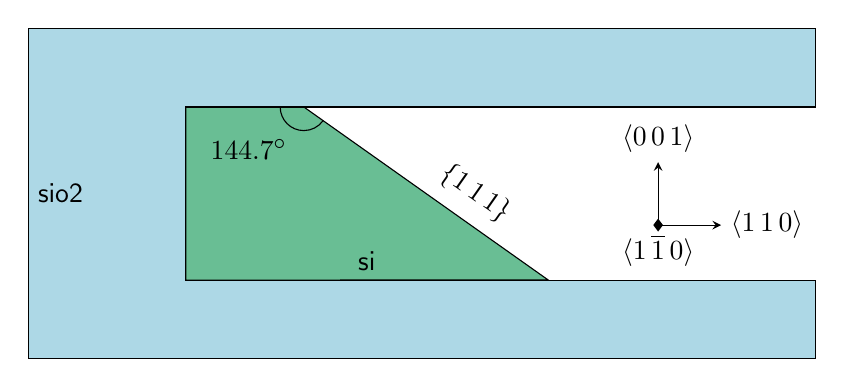
\begin{tikzpicture}
            \filldraw[fill=Si_green] (2cm, 0cm) -- (2cm, 22mm) -- (3.5cm, 22mm) -- ++ (-35.3:3.8cm) node[midway, anchor=west]{\rotatebox{-35.3}{\hkl{1 1 1}}} --  node[midway, anchor=south] {\acs{si}} cycle;
            \filldraw[fill=SiO2_blue] (0cm, -10mm) -- (10cm, -10mm) -- (10cm, 0cm) -- (2cm, 0mm)-- (2cm, 22mm) -- (10cm, 22mm) -- (10cm, 32mm) -- (0cm, 32mm) --  node[midway, anchor=west] {\acs{sio2}} cycle; 
            \draw (3.2cm, 22mm) arc [start angle = 180, end angle = 324.7, radius = 3mm] node[midway, anchor = north east]{\qty{144.7}{\degree}};
            \draw[-stealth] (8cm, 7mm) node[anchor=north] {\hkl<1 -1 0>} -- ++ (90:0.8cm) node[anchor=south] {\hkl<0 0 1>};
            \draw[-stealth] (8cm, 7mm) -- ++ (0:0.8cm) node[anchor=west] {\hkl<1 1 0>};
            \node[mark size=2pt] at (8, 7mm) {\pgfuseplotmark{diamond*}};
        \end{tikzpicture}
    }
    \caption{Wafer symmetry and microstructure design. \subref{subfig:001wafer_directions} shows the in-plane low-index crystalline directions in a \hkl(0 0 1) wafer, using a \qty{90}{\degree} arc centred around the notch that indicates the in-plane direction \hkl[1 1 0]. The rest of the directions can be deduced by the symmetry defined by the four-fold axis perpendicular to the wafer plane. \subref{subfig:enterprise_design} illustrates two different microstructure designs, complemented by a scale bar and an in-plane orientation guide. The black designs were transferred to the device \acs{si} layer of the \acs{soi} wafer, while the red designs marked the position of the template openings. \subref{subfig:enterprise_etchback} is a drawing of the \acs{si} seed area showing its configuration after etch-back for a structure orientated along an in-plane \hkl<1 1 0> direction.}
    \label{fig:001_Templat5e_Design}
\end{figure}

The orientation of the \acs{tase} template on the \acs{si} \hkl(0 0 1) surface, and therefore the crystalline direction along which the growth will take place, is the first key factor in determining the final shape of the crystal. In the \acs{si} space group \num{227} \cite{osti_si}, the \hkl<0 0 1> vector contains a four-fold axis, represented by a square dot in Figure~\ref{subfig:001wafer_directions}. If we were to examine the possible in-plane directions within an arbitrary \qty{90}{\degree} angle, we would find them repeated three more times in the remaining in-plane \qty{270}{\degree} arc because of this symmetry element. Figure~\ref{subfig:001wafer_directions} shows this principle applied to the \hkl(0 0 1) wafer used to fabricate the first samples. By drawing a \qty{90}{\degree} angle around the notch indicating the \hkl[1 1 0] direction and highlighting the low-index in-plane directions, the two equivalent \hkl[0 1 0] and \hkl[1 0 0] directions define the edges of the arc. Although the cubic III-V semiconductor phase is zincblende (space group \num{216}) \cite{wyckoff1963crystal, osti_gaas_zb, osti_inas_zb, osti_inp_zb}, equivalent symmetry considerations can be made, provided the polar nature of the compound is taken into account.
\par
Most previous \acs{tase} nanowire growth experiments have used the \hkl<1 1 0> vector as the primary in-plane growth axis \cite{Brunelli2019, Knoedler2017, Borg2017}. Therefore, this direction was selected as a starting point to analyse the growth results. Figure~\ref{subfig:enterprise_design} shows the two designs divided by colour in the two \acf{ebl} exposures during fabrication with scale and direction relative to the crystal. For the first design, the black pattern comprises a series of \num{11} nanowires and a back anchor in a comb-like structure. These, while maintaining a constant wire length, were designed in multiple wire widths ranging from \qty{50}{\nano\metre} to \qty{500}{\nano\metre}. In contrast, the second design is shaped as a capital "T" with a wire thickness ranging from \qty{50}{\nano\metre} to \qty{400}{\nano\metre}. These designs are transferred onto the \acs{si} layer by selectively etching the superfluous material around them. Subsequently, the resulting structures are encapsulated in a \acs{sio2} layer that forms the template. \acs{ebl} is then used to define the area of the template to be opened (in red in Figure~\ref{subfig:enterprise_design}).
\par
Figure~\ref{subfig:enterprise_etchback} shows the situation of the \acs{si} seed of one of the nanowires after template opening and etch-back of the microstructured \acs{si} device layer. It is encased on all but one side by the oxide template and the buried oxide. It presents a surface composed of one (or, as seen experimentally, two, with one being larger than the other in most seed surfaces) \hkl{1 1 1} facets because of the chemistry of the \acs{tmah} etch, which is slower on this densely-packed facet \cite{Zubel2012}. The acute angle that this type of facet forms with the template can easily result in unwanted effects, such as incomplete template filling in the seed area \cite{Scherrer2022}. 

\subsection{Simple precursor switching sequence}

\begin{figure}
    \centering
    \subcaptionbox{
    Growth recipe \cite{Brugnolotto2023}.
    \label{subfig:recipe1}
    }{
    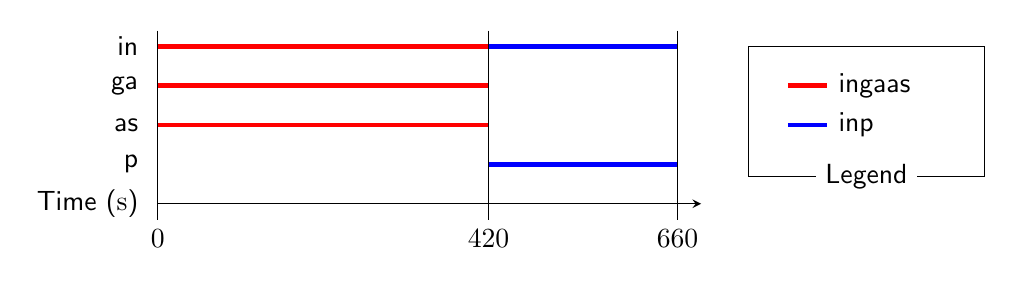
\begin{tikzpicture}
    \begin{scope}
    % lines
        \node [label={[label distance=0]180:\acs{in}}] at (0, 0) {};
        \draw [red, ultra thick] (0, 0) -- (4.2, 0);
        \draw [blue, ultra thick] (4.2, 0) -- (6.6, 0);
        \node [label={[label distance=0]180:\acs{ga}}] at (0, -0.5) {};
        \draw [red, ultra thick] (0, -0.5) -- (4.2, -0.5cm);
        \node [label={[label distance=0]180:\acs{as}}] at (0, -1) {};
        \draw [red, ultra thick] (0, -1) -- (4.2, -1);
        \node [label={[label distance=0]180:\acs{p}}] at (0, -1.5) {};
        \draw [blue, ultra thick] (4.2, -1.5) -- (6.6, -1.5);
    % labels and markers for the timescale
        \node [label={[label distance=0]180:Time (\second)}] at (0, -2) {};
        \draw [-stealth] (0, -2) -- (6.9, -2);
        \draw [] (0, 0.2) -- (0, -2.2) node[anchor = north] {\num{0}};
        \draw [] (4.2, 0.2) -- (4.2, -2.2) node[anchor = north] {\num{420}};
        \draw [] (6.6, 0.2) -- (6.6, -2.2) node[anchor = north] {\num{660}};
    \end{scope}
    \begin{scope} [shift={(8cm, -0.5)}]
        \draw [red, ultra thick] (0, 0) -- (0.5, 0) node[anchor = west, text=black] {\acs{ingaas}};
        \draw [blue, ultra thick] (0, -0.5) -- (0.5, -0.5) node[anchor = west, text=black] {\acs{inp}};
        \draw (-0.5, 0.5) -- (2.5, 0.5) -- (2.5, -1.15) -- node[midway, fill=white] {Legend} (-0.5, -1.15) -- cycle;
    \end{scope}
    %\begin{scope}[yshift = -4cm]
    %    \node [label={[label distance=0cm]180:\acs{in}}] at (0, 0) {};
    %    \draw [red, ultra thick] (0, 0) -- (20cm, 0);
    %    \node [label={[label distance=0cm]180:\acs{ga}}] at (0, -0.5cm) {};
    %    \draw [red, ultra thick] (0, -0.5cm) -- (20cm, -0.5cm);
    %    \node [label={[label distance=0cm]180:\acs{as}}] at (0, -1cm) {};
    %    \draw [red, ultra thick] (0, -1cm) -- (20cm, -1cm);
    %    \node [label={[label distance=0cm]180:\acs{p}}] at (0, -1.5cm) {};
    %    \draw [red, ultra thick] (0, -1.5cm) -- (20cm, -1.5cm);
    %    \node [label={[label distance=0cm]180:Time (\second)}] at (0, -2.5cm) {};
    %    \draw [black, -stealth] (0, -2.5cm) -- (20cm, -2.5cm);
    %\end{scope}
    \end{tikzpicture}
    }
    \subcaptionbox{
    \qty{52}{\degree} tilted image of III-V nanowires.
    \label{subfig:comb_sample1}
    }{\begin{tikzpicture}
        \node[inner sep=0pt] (image) at (0,0) {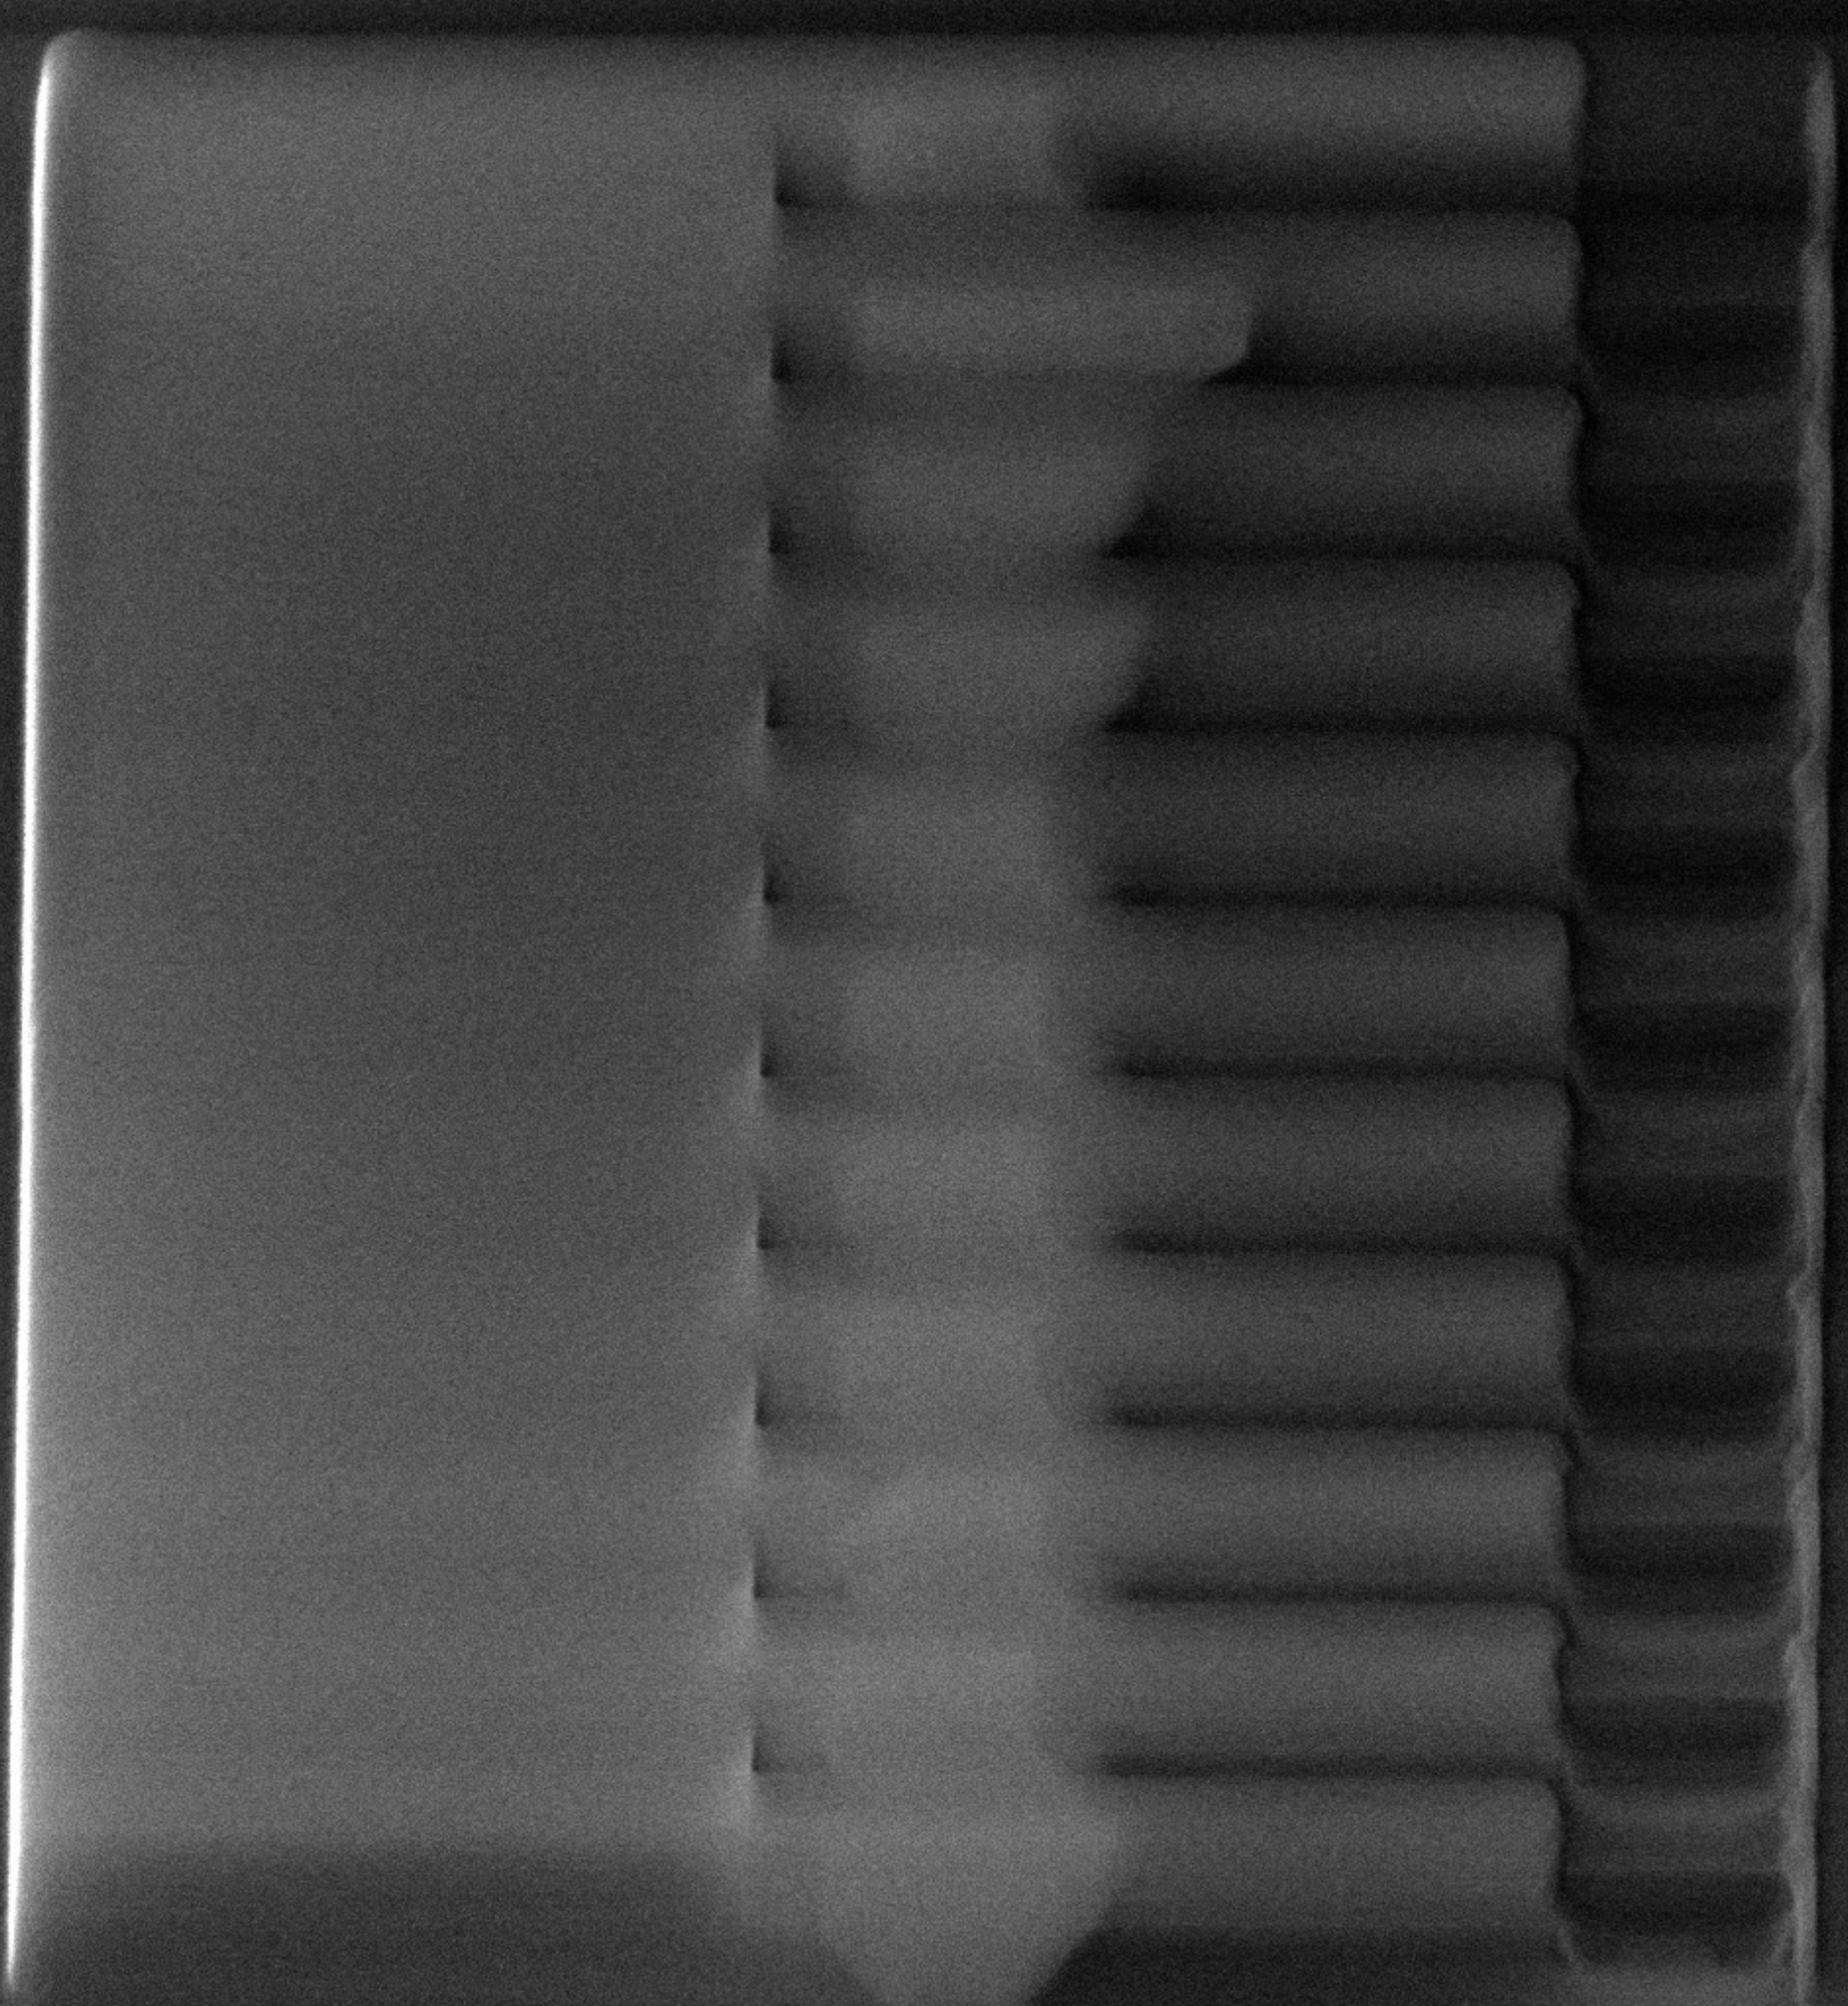
\includegraphics[width=0.6\textwidth]{3_Growth/Comb_Array_001.pdf}};
        \draw [|-|, white, very thick] (-4.6, -4) -- (-1, -4) node [midway, anchor=south] {\qty{1}{\micro\metre}};
        \draw [|-|] (-4.8, -5.5) -- (-0.4, -5.5) node [midway, anchor=north]{\acs{si} backbone and seed};
        \draw [|-|] (-0.4, -5.5) -- (0.9, -5.5) node [midway, anchor=north]{III-V};
        \draw [|-|] (0.9, -5.5) -- (3.2, -5.5) node [midway, anchor=north]{template};
        \draw [|-|] (3.2, -5.5) -- (4.7, -5.5) node [midway, anchor=north]{opening};
    \end{tikzpicture}
    }
    \caption{Growth of the first sample. \subref{subfig:recipe1} Is the diagram representing the growth recipe for a simple single-heterointerface III-V wire \cite{Brugnolotto2023}. Each line represents an active flow of precursor into the reactor. The colour of the horizontal lines represents the target material. \subref{subfig:comb_sample1} Is an \acs{sem_m} image of an \num{11}-nanowire array. The \acs{si} seed, III-V segment, empty template, and template opening are visible from left to right.}
    \label{fig:sample1_growth}
\end{figure}

The second key factor in determining the shape of the growing crystal is the individual growth rate of each facet. Growth conditions, including temperature, precursor molar flow, III/V ratios, and chemical species, are the key to determining the low-index facet growth rate \cite{Borg2015, Elsner1992}.
\par
After all the fabrication and pre-processing steps, the growth of III-V material occurs in an \acf{mocvd} reactor at \qty{580}{\degreeCelsius}. The recipe used for the first growth experiment is shown in Figure~\ref{subfig:recipe1}. The objective of this growth run was to study the evolution of growth in a simple sample to evaluate the effects of the growth parameters on the end morphology of the two material layers. Two different III-V material layers were grown for this sample: the deposition times of \qty{420}{\second} and \qty{240}{\second} were chosen for the \acs{ingaas} and \acs{inp} layer, respectively. Table~\ref{tab:sample1_ratios} summarises the V/III molar ratios loaded into the reactor. These were chosen according to those used in previous experiments, which were meant to aid in recognising patterns that could be improved upon during growth without unexpectedly influencing parameters such as nucleation yield and growth rates.

\begin{table}
    \centering
    \caption{V/III molar ratios injected in the reactor during each material deposition step \cite{Brugnolotto2023_2}.}
    \begin{tabular}{l|c}
        Material & V/III ratio \\ \hline \hline
        InGaAs  & 234\\
        InP     & 29\\ \hline
    \end{tabular}
    \label{tab:sample1_ratios}
\end{table}

The \acs{sem_m} image in Figure~\ref{subfig:comb_sample1} shows a comb array with \num{11} nanowires. The structure segments are marked: on the right side of the image, the holes through which the precursors entered the templates are visible. The image was captured with the sample fixed on a stage that was tilted \qty{52}{\degree} with respect to the \hkl<0 0 1> before \acs{fib} cutting. The shape of the end-faced of each nanowire is visible due to the tilt, with most wires terminating with a \hkl{1 1 1}\(_B\) facet. Only one of the wires, the second one from the top, appears to have a different end-facet. The third wire from the bottom presents an interesting (but not unique, as shown in \cite{Scherrer2022}) situation where the growing crystal leaves the seed partially uncovered. Two \hkl{1 1 0} facets form an arrowhead-like shape, indicating the presence of faster growth in the \hkl<1 1 1> direction compared to the \hkl<1 1 0> directions immediately after nucleation.

\subsection{\texorpdfstring{\acs{fib} lamella fabrication}{FIB lamella fabrication}}

\begin{figure}
    \centering
    \subcaptionbox{
        \acs{sem_m} image of an electron transparent lamella \cite{Brugnolotto2023}.
        \label{subfig:FIB_cut}
        }{\begin{tikzpicture}
            \node[inner sep=0pt] (image) at (0,0) {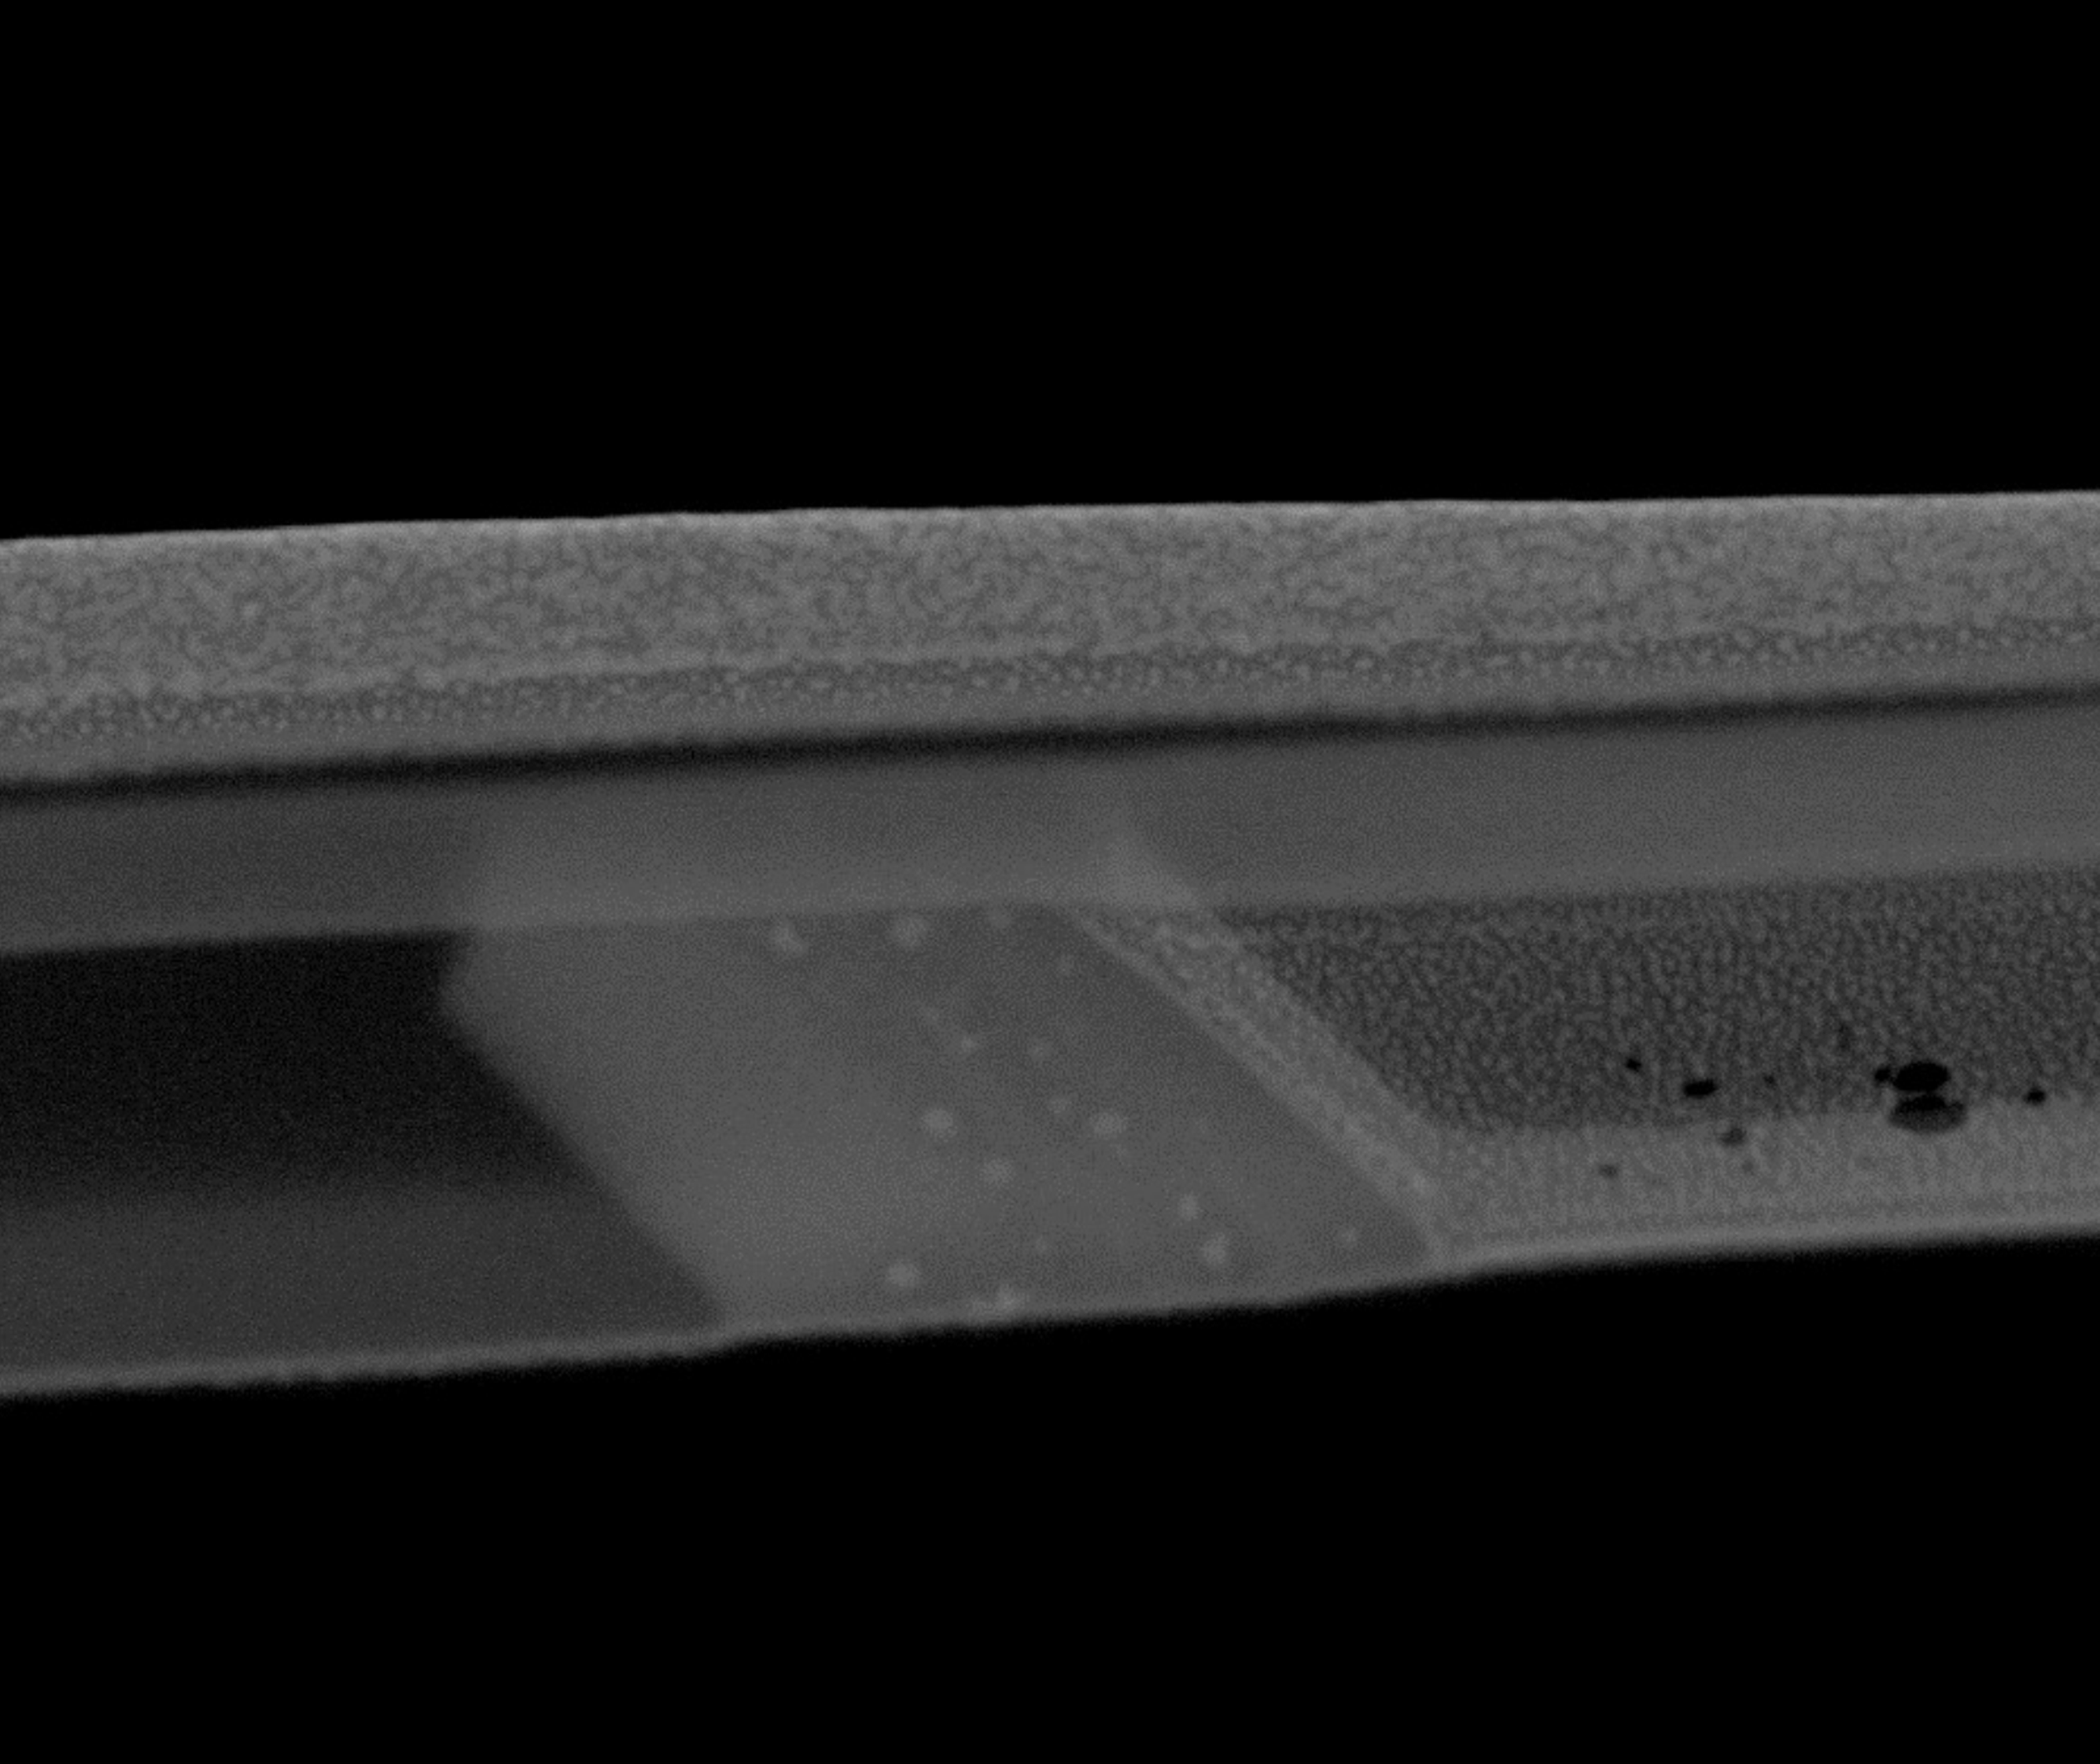
\includegraphics[width=0.48\textwidth]{3_Growth/FIB_Cut.pdf}};
            \node [text=white,] at (-2, -2.5) {\acs{sio2}};
            \node [text=white] at (2, 0.3) {\acs{sio2}};
            \node [text=white] at (0, -0.7) {III-V};
            \node [text=white] at (-2.5, -1) {\acs{si}};
            \node [text=white] at (0, 1) {\ce{Pt}};
            \node [text=white] at (2, -0.5) {Void};
        \end{tikzpicture}
    }
    \subcaptionbox{
        Cutting strategy for a cross section in a \hkl(0 0 1) substrate.
        \label{subfig:FIB_cut_strategy}
        }{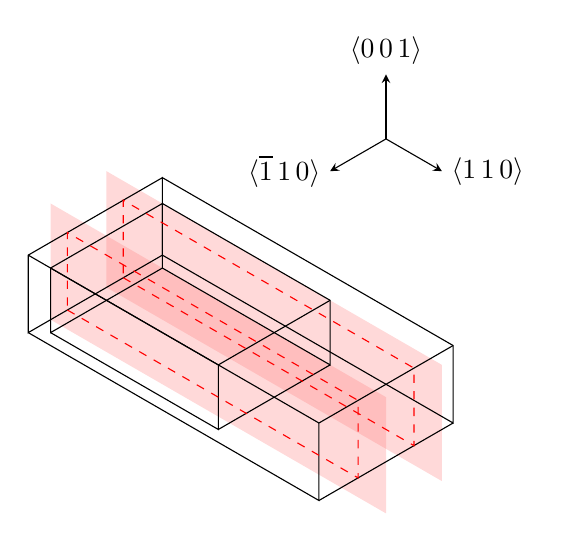
\begin{tikzpicture}[isometric]
            \path [fill=red!50!, fill opacity=0.3] (-0.5, -0.3, 0.5) -- (-0.5, 1.5, 0.5) -- (5.5, 1.5, 0.5) -- (5.5, -0.3, 0.5) -- cycle;
            \path [fill=red!50!, fill opacity=0.3] (-0.5, -0.3, 1.5) -- (-0.5, 1.5, 1.5) -- (5.5, 1.5, 1.5) -- (5.5, -0.3, 1.5) -- cycle;
            
            \draw (0, 0, 0) -- (0, 0, 2) -- (0, 1, 2) -- (0, 1, 0) -- cycle;
            \draw (0, 0, 0) -- (3, 0, 0) -- (3, 1, 0) -- (0, 1, 0);
            \draw (0, 0, 2) -- (3, 0, 2) -- (3, 1, 2) -- (0, 1, 2);
            \draw (3, 0, 0) -- (3, 0, 2);
            \draw (3, 1, 0) -- (3, 1, 2);
            
            \draw (-0.2, 0, -0.2) -- (-0.2, 0, 2.2) -- (-0.2, 1.2, 2.2) -- (-0.2, 1.2, -0.2) -- cycle;
            \draw (-0.2, 0, -0.2) -- (5, 0, -0.2) -- (5, 1.2, -0.2) -- (-0.2, 1.2, -0.2);
            \draw (-0.2, 0, 2.2) -- (5, 0, 2.2) -- (5, 1.2, 2.2) -- (-0.2, 1.2, 2.2);
            \draw (5, 0, -0.2) -- (5, 0, 2.2);
            \draw (5, 1.2, -0.2) -- (5, 1.2, 2.2);
            
            \draw [red, dashed] (-0.2, 0, 0.5) -- (5, 0, 0.5) -- (5, 1.2, 0.5) -- (-0.2, 1.2, 0.5) -- cycle;
            \draw [red, dashed] (-0.2, 0, 1.5) -- (5, 0, 1.5) -- (5, 1.2, 1.5) -- (-0.2, 1.2, 1.5) -- cycle;

            \draw [-stealth] (5, 5, 1) -- (6, 5, 1) node[anchor=west]{\hkl<1 1 0>};
            \draw [-stealth] (5, 5, 1) -- (5, 6, 1) node[anchor=south]{\hkl<0 0 1>};
            \draw [-stealth] (5, 5, 1) -- (5, 5, 2) node[anchor=east]{\hkl<-1 1 0>};
        \end{tikzpicture}
    }
    \caption{\acs{fib} cut of a lamella from a \hkl<0 0 1> \acs{soi} wafer. \subref{subfig:FIB_cut} shows the \acs{sem_m} image of a thinned electron-trasparent lamella. The various materials are marked, and the structure is discernible. \subref{subfig:FIB_cut_strategy} shows how the cut is made within the context of the crystalline and growth directions. The red-shaded planes show that we select the cut to expose the sides of the wire in correspondence to a \hkl{-1 1 0} plane if we label the template axis as a \hkl<1 1 0> direction.}
    \label{fig:001_FIB}
\end{figure}

A high-resolution analytical method is needed to analyse the type of structures shown in Figure~\ref{subfig:enterprise_design}. Indeed, their small size means that, for example, X-ray analysis with laboratory-sized tools is unfeasible. Instead, microscopy techniques are particularly powerful, with high-end \acf{tem_i} or \acf{stem_i} able to resolve features up to atomic resolution and provide important structural information. However, an electron-transparent lamella is required to analyse material layers and investigate the morphology of internal heterointerfaces. \Acf{fib} tools can create these <\qty{100}{\nano\metre} thin semiconductor cross sections. In this study, an FEI Helios NanoLab 450S was used.
\par
Figure~\ref{subfig:FIB_cut} shows how one lamella looks once \acs{fib} cutting is complete. This image is perfect for showcasing the various material portions of the sample while retaining a three-dimensional view, which is lost in the later \acs{stem_m} analysis. The \acl{si} seed is visible on the left, followed by the III-V material layer, which appears brighter in the centre of the image. On the exposed surface of this layer, two areas can be characterised and distinguished by the presence of small \acl{in} droplets (on the right side) and their absence. These \acl{in} droplets are commonly formed during the ion milling of \acl{inp} at the \acs{fib} tool. On the right side, the empty template is filled with a \ce{Pt} lace structure formed when the protection layer was deposited before the lamella was cut from the chip. The upper and lower interfaces of the template are visible in this image, appearing as two ribbons or bands above and below the \acs{si}/III-V/Void structure. In particular, the upper interface is the most visible; they can be easily spotted by looking at the \acs{si} region. What remains of the \ce{Pt} protective layer is also noticeable as a bright region at the very top of the structure.
\par
The objective of the cut strategy shown in Figure~\ref{subfig:FIB_cut_strategy} is two-fold. The first aim is to provide a lamella that showcases both the seed and end facets to evaluate the evolution of the growth front, and the second is to have access to a low-index facet that can provide structural information on the effectivity of the lattice. For the zincblende phase, the second criterion is satisfied by \hkl{1 1 0} facets \cite{Dasilva2017}, and for a \hkl{0 0 1} \acs{soi} there is an in-plane \hkl[-1 1 0] direction perpendicular to the \hkl[1 1 0] direction along which the template is orientated. This means that a simple cross-section along the wire allows access to the maximum information about the nanowire.

\subsection{\texorpdfstring{\acs{stem_m} analysis}{STEM analysis}}

\begin{figure}
    \centering
    \subcaptionbox{
        \acs{bf}-\acs{stem_m} overview of a III-V nanowire cross-section.
        \label{subfig:sample1_cross-sec}
        }{\begin{tikzpicture}
            \node[inner sep=0pt] (image) at (0,0) {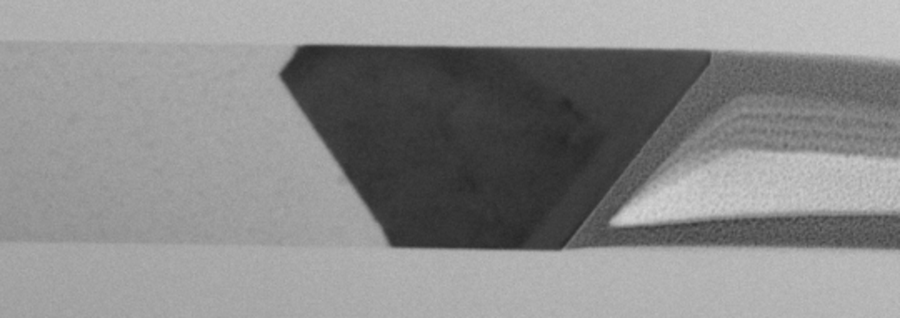
\includegraphics[width=\textwidth]{3_Growth/Sample1_Overview.pdf}};
            \draw [red] (1.25, -1.63) -- (2.9, 0.5); %1.65, 2.13
            \draw [red, dashed] (0.95, 1.93) -- (2.9, 0.5) -- (3.35, 1.1) -- (2.2, 1.93);
            \draw [orange] (2, -1.63) -- (4.65, 1.7) -- (4.7, 1.93);
            \draw [yellow] (-3.3, 1.2) rectangle (-2.7, 1.8);
            \draw [|-|, very thick] (-7.4, -2.5) -- (-4, -2.5) node [midway, anchor=south] {\qty{1}{\micro\metre}};
            \node [text=white] at (5.5, 1.5) {\ce{Pt}};
            \node at (-2, -2) {\acs{sio2}};
            \node at (2, 2.4) {\acs{sio2}};
            \node [text=white] at (0, -0.7) {\acs{ingaas}};
            \node [text=white] at (3.5, 1.5) {\acs{inp}};
            \node at (-2.5, -0.7) {\acs{si}};
            \node at (5, -0.5) {Void};
        \end{tikzpicture}
    }
    \subcaptionbox{
        \acs{eds} map: red-\acs{in}, green-\acs{si}, blue-\acs{ga}.
        \label{subfig:s1_III_EDS}
        }{\begin{tikzpicture}
            \node[inner sep=0pt] (image) at (0,0) {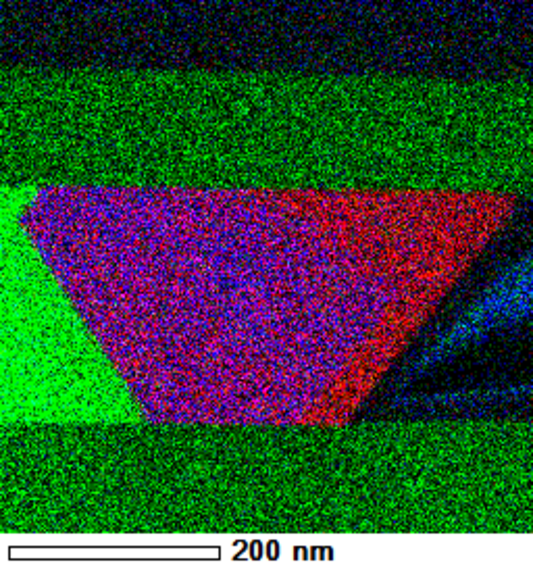
\includegraphics[width=0.45\textwidth]{3_Growth/s1_III_EDS.pdf}};
        \end{tikzpicture}
    }
    \subcaptionbox{
        \acs{eds} map: red-\acs{as}, green-\acs{p}, blue-\acs{in}.
        \label{subfig:s1_V_EDS}
        }{\begin{tikzpicture}
            \node[inner sep=0pt] (image) at (0,0) {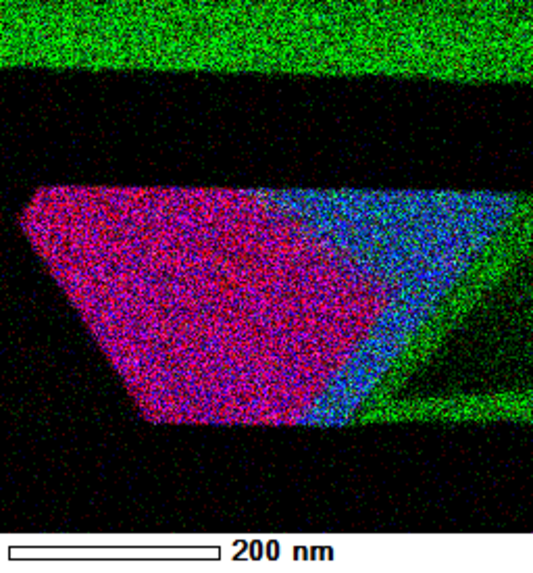
\includegraphics[width=0.45\textwidth]{3_Growth/s1_V_EDS.pdf}};
        \end{tikzpicture}
    }
    \subcaptionbox{
        \acs{bf}-\acs{stem_m} detail of the \acs{si}/\acs{ingaas} interface.
        \label{subfig:si-ingaas_s1}
        }{\begin{tikzpicture}
            \node[inner sep=0pt] (image) at (0,0) {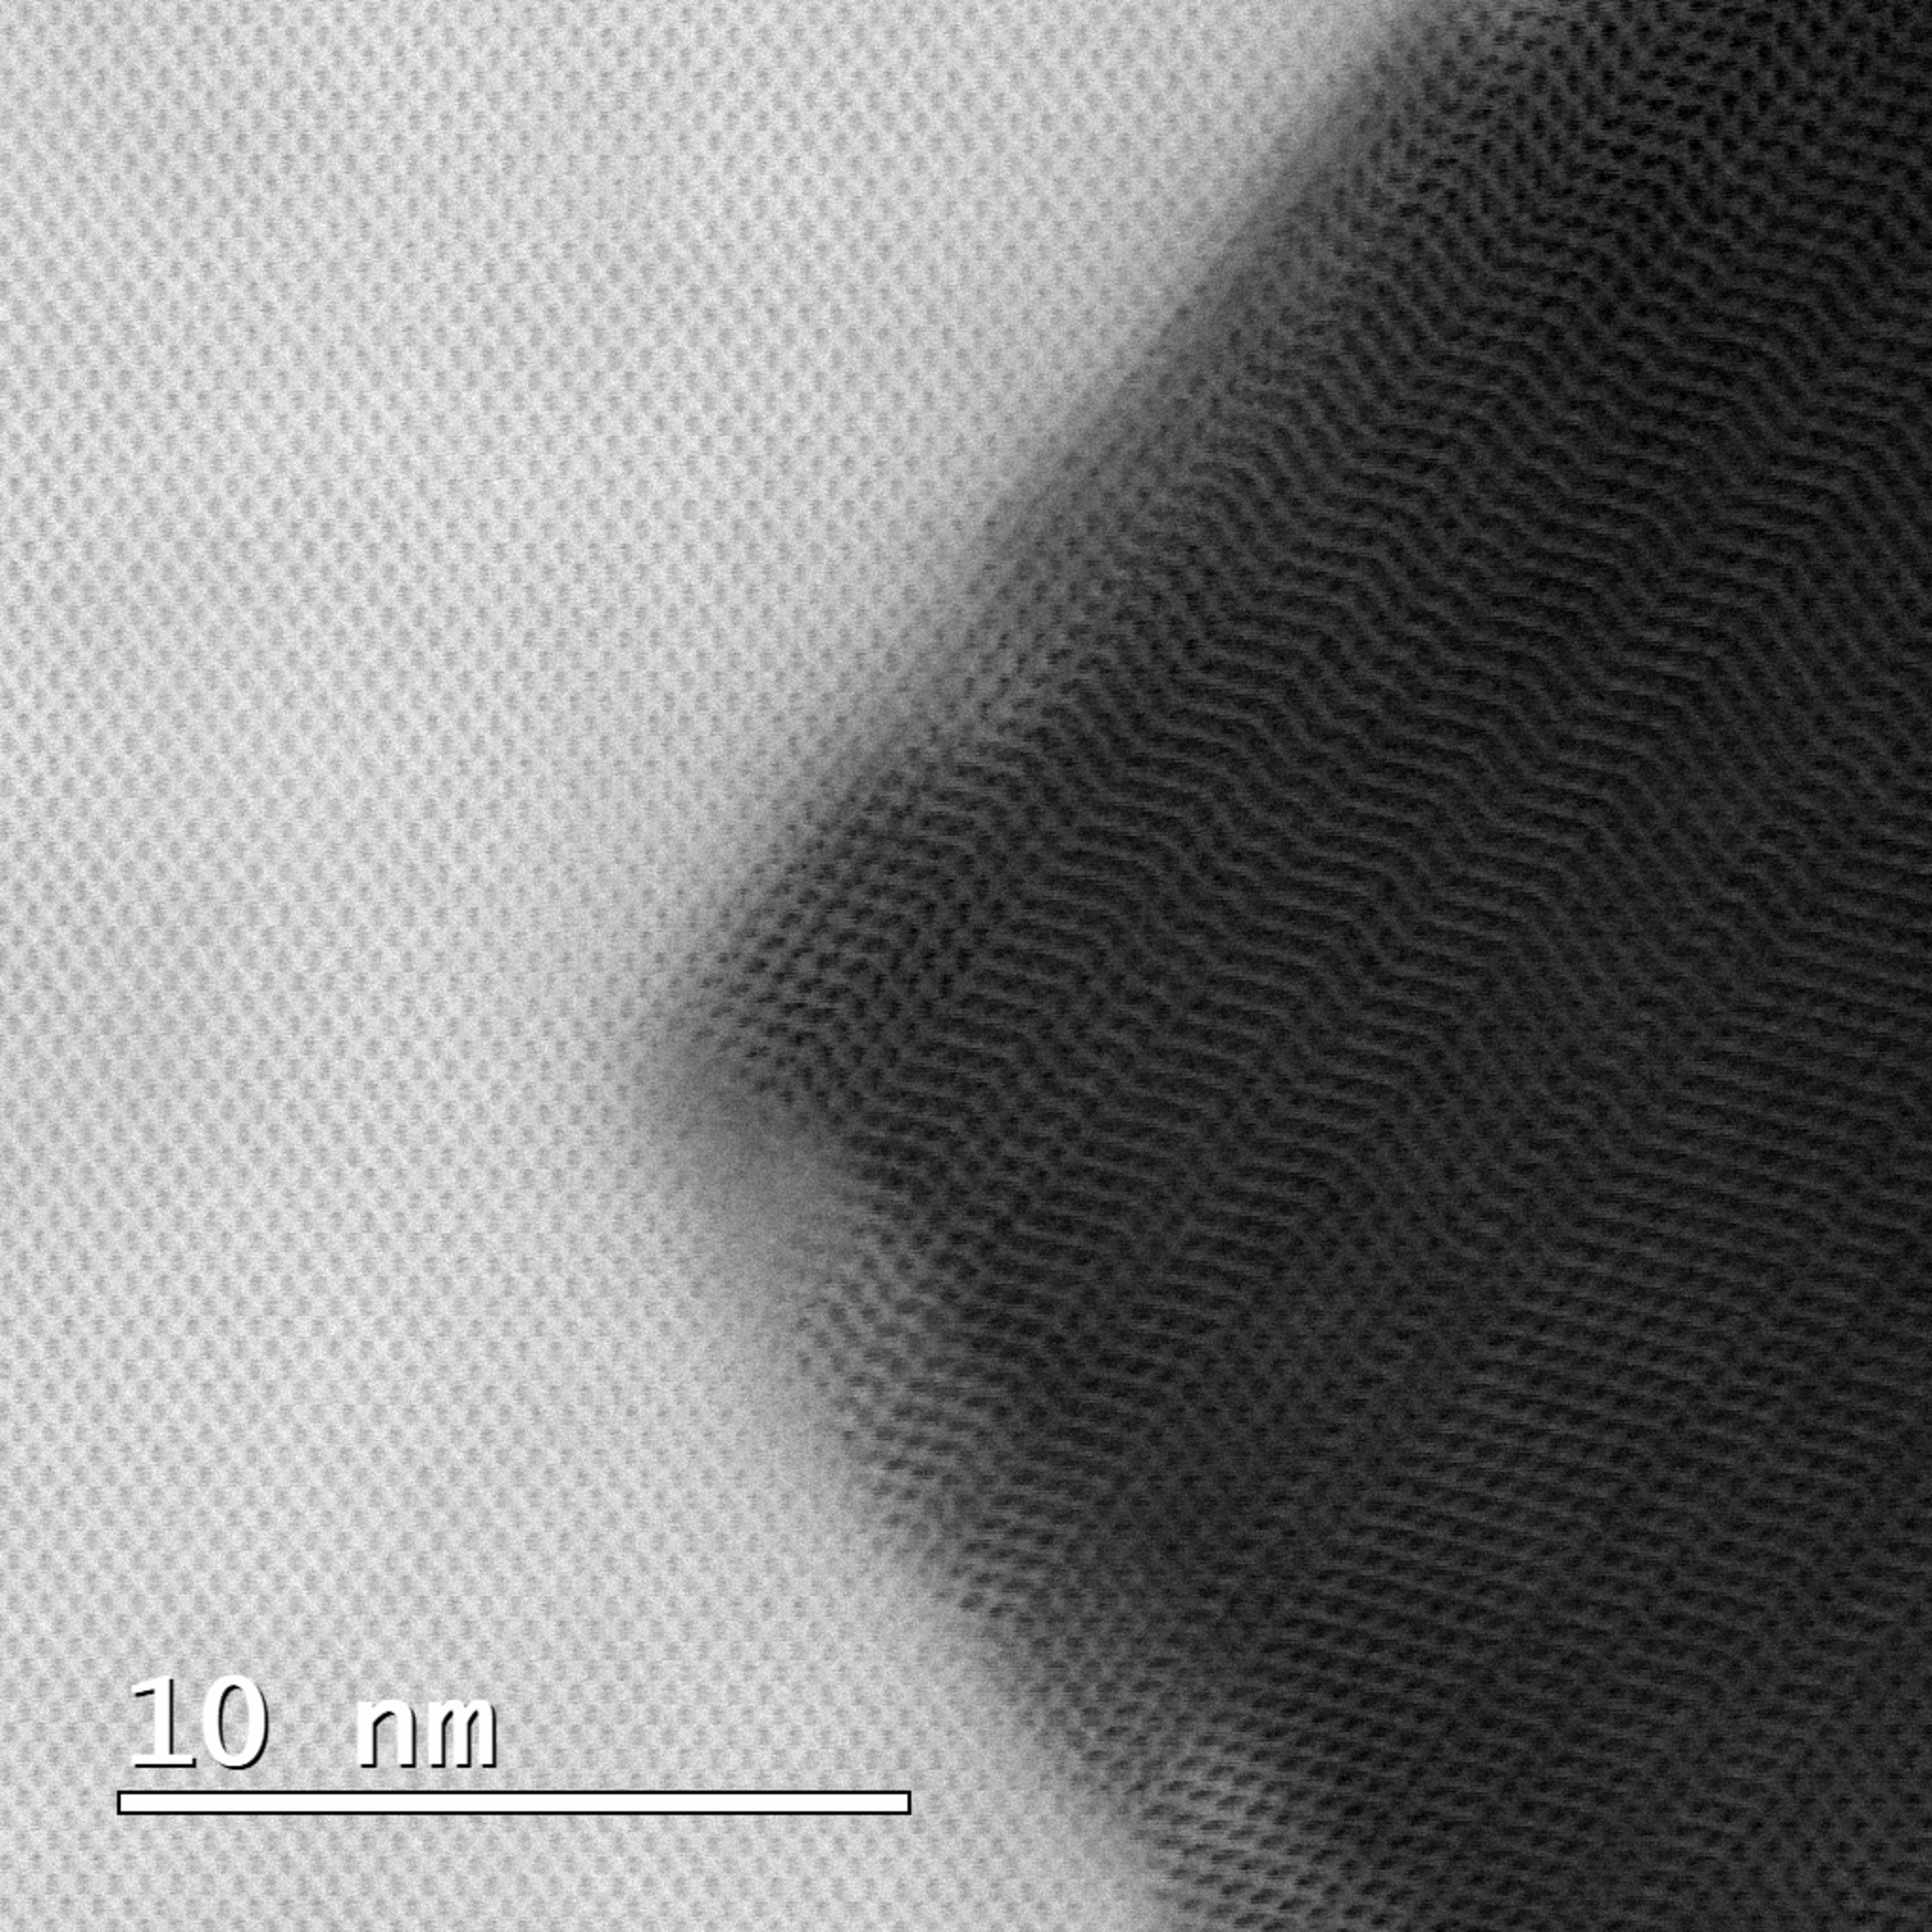
\includegraphics[width=0.45\textwidth]{3_Growth/Si_interface_sample1.pdf}};
            \node [white] at (2, -1) {\acs{ingaas}};
            \node at (-3, 3) {\acs{si}};
        \end{tikzpicture}
    }
    \caption{Overview, composition analysis, and detail of the seed/\acs{ingaas} interface.}
    \label{fig:sample1}
\end{figure}

The bottom-most wire of the array in Figure~\ref{subfig:comb_sample1} was chosen for investigation. Once the \acs{fib} cut was complete, the resulting lamella was cleaned in an oxygen plasma for \qty{30}{s} before being loaded in a JEOL ARM 200F \acl{stem_i}. Figure~\ref{subfig:sample1_cross-sec} shows an overview image of the lamella imaged with the \acf{bf} detector of the \acs{stem_m}. The difference in atomic number gives contrast to the image through what is known as Z-contrast: material composed of heavier atoms will appear darker in a \acs{bf} image, and vice versa in an \acf{adf} or \acf{haadf} image. Therefore, the darkest area of the sample is the \acs{ingaas} layer, as its III and V components have a high atomic number. \acs{inp} appears a bit brighter given that the V element, \acl{p}, is light. The \acs{si} and \acs{sio2} layers are very bright in comparison, as the small \acs{si} and \ce{O} atoms allow the transmission of a higher portion of the beam. The contrast of the \acs{fib}-deposited \ce{Pt} is modulated by its thickness and lower density. The Z-contrast's compositional clues are confirmed by spectroscopic analysis in Figure~\ref{subfig:s1_III_EDS} and Figure~\ref{subfig:s1_V_EDS}.
\par
\paragraph{Spectroscopic analysis}Figure~\ref{subfig:s1_III_EDS} shows a low-resolution compositional map created with the \acf{eds} data from the sample in Figure~\ref{subfig:sample1_cross-sec}. The map is colour-coded with each colour representing the intensity of an element-specific spectroscopic line processed to consider the cross-section of each transition. This creates the compositional map. Areas that appear more red have a higher \acl{in} concentration, those that appear green have a high \acs{si} content, and those with a blue tinge contain \acl{ga}. The brightness of its colour carries information regarding the amount of each element present in each region. For example, the \acs{si} signal is stronger in the seed area on the left of the image and fainter in the top and bottom \acs{sio2} template and buried oxide areas. \Acl{in} signal is present throughout the III-V area, as expected given the two \acs{ingaas} and \acs{inp} layers. The \acl{ga} signal is mostly confined to the \acs{ingaas} layer, but a small blue tint can be noticed in correspondence with the outer \ce{Pt} region inside the template on the right centre of the map. This is due to the \acs{fib} processing causing redeposition. Indeed, some green dots from the redeposited \acl{si} can also be spotted in that map area. The absence of \acl{in} signal could be attributed to the tendency of this material to form droplets, as seen in Figure~\ref{subfig:FIB_cut}.
\par
Another \acs{eds} map of the lamella in Figure~\ref{subfig:sample1_cross-sec} investigating the distribution of V elements is shown in Figure~\ref{subfig:s1_V_EDS}. Here, \acl{as} appears in red, \acl{p} in green, and \acl{in} in blue. The \acl{in} signal allows for the determination of the III-V area, as it is present in both \acs{inp} and \acs{ingaas}. The \acl{as} signal defines the \acs{ingaas} area, and the green dots revealing the presence of \acl{p} are also present in the remaining \acs{in}-rich area. What appears, upon first examination, to be further \acl{p} high concentration in the \acs{fib}-deposited \ce{Pt} is also noticeable. However, this signal can be better explained by examining the energy at which the \acl{p} K\(_\alpha\) line is located. Indeed, the \acs{p} K\(_\alpha\) line at \qty{2.013}{\kilo\eV} is very close to the \ce{Pt} M line, which falls at \qty{2.048}{\kilo\eV}. These two energies are too close for the two peaks to be distinguished when peak width and spectral resolution are taken into account, generating the "fake" \acl{p} signal in the platinum layers.
\par
\paragraph{Heterointerfaces}This sample presents three interfaces of interest: \acs{si}/\acs{ingaas}, \acs{ingaas}/\acs{inp}, and \acs{inp}/empty template. Figure~\ref{subfig:si-ingaas_s1} shows the first interface at the "V" corner marked with a yellow square in Figure~\ref{subfig:sample1_cross-sec}. Here, the epitaxial relation between the two lattices is visible. The surface of the \acs{si} seed has some roughness, as made evident by the varying intensity of the \acs{ingaas} image in the first \num{6} III-\acs{as} layers. \Acl{rtp}s parallel to the upper \hkl{1 1 1} \acs{si} facet are also visible in this high-resolution image. The shape of this first interface is defined by the \acs{tmah} etch-back before growth, but the next interface, between \acs{ingaas} and \acs{inp}, is determined by the growth parameters in the reactor. Its shape is consistent with that seen in \cite{Scherrer2022, Borg2017, Borg2015}, with a lower \hkl{1 1 1} facet (marked with a red full line) and an upper \hkl{1 1 0} facet (traced on its expected position in a dashed red line), which is likely one of two. Interestingly, this \hkl{1 1 0} facet disappears almost completely after the growth of the \acs{inp} layer, leaving only a long \hkl{1 1 1} facet and a smaller \hkl{1 1 0} facet at the top. The \hkl{1 1 1} facet is parallel to the \acs{rtp}s and, therefore, the upper \acs{si} interface. Looking back at the array of nanowires in Figure~\ref{subfig:comb_sample1}, the selection of which starting \hkl{1 1 1} facet the end-facet is parallel to appears to be random.
\par

\begin{table}
    \centering
    \caption{Growth rates for the first grown sample.}
    \begin{tabular}{l|c c c}
                    & \multicolumn{3}{c}{Growth rates (\nmmin)}                                                                                                   \\
       Layer        & \hkl<1 1 1>                                   & Longest distance                              & Shortest distance                           \\ \hline \hline
       \acs{ingaas} & \num[separate-uncertainty=true]{46.5 (0.1)}   & \num[separate-uncertainty=true]{51.8 (0.2)}   & \num[separate-uncertainty=true]{20.0 (0.2)} \\
       \acs{inp}    & \num[separate-uncertainty=true]{9.1 (0.2)}    & \num[separate-uncertainty=true]{57.2 (0.8)}   & \num[separate-uncertainty=true]{9.1 (0.2)}  \\ \hline
    \end{tabular}
    \label{tab:sample1_growth_rates}
\end{table}

\paragraph{Growth rates} An attempt to estimate the growth rate of \acs{ingaas} and \acs{inp} can be made. However, multiple reference points can be taken to measure between them because the shape of the seed and end facet are complex. Three different measurements were made for each layer: \hkl<1 1 1>, longest distance, and shortest distance; the first category means that the distance between the two parallel \hkl{1 1 1} facets is measured to calculate the growth rate. For \acs{inp}, the \hkl<1 1 1> and shortest distance growth rates coincide. For the \hkl<1 1 1> growth rates, the difference between \acs{ingaas} and \acs{inp} is particularly high, and so is the difference between the longer distance and the \hkl<1 1 1> growth rates of \acs{inp}. This suggests that the \acs{inp} growth rate in the \hkl<1 1 0> direction is higher than that in the \hkl<1 1 1> direction.

\section{Introduction of thin material layers}

Regarding growth dynamics, the main finding from the sample in Figure~\ref{fig:sample1} is the trend towards stabilisation of the \hkl{1 1 1} growth front during \acs{inp} growth. However, many optoelectronic devices rely on harnessing the properties of quantum confinement structures, and there is no one thin enough layer in sample 1 to constitute one. Therefore, an effort was made to introduce short material deposition segments in the growth recipe and study how they modified and manifested in the final nanowire morphology and composition.

\subsection{Growth recipe for the introduction of short material segments.}

\begin{figure}
    \centering
    \subcaptionbox{
    Growth recipe for sample 2 \cite{Brugnolotto2023}.
    \label{subfig:recipe2}
    }{
    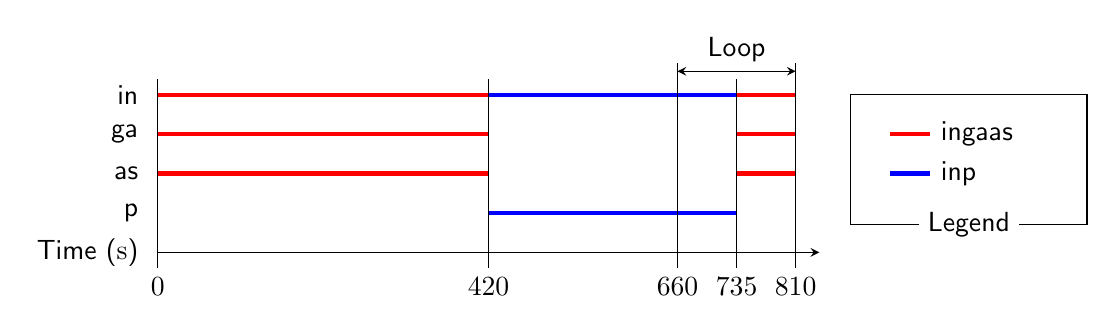
\begin{tikzpicture}
    \begin{scope}
    % lines
        \node [label={[label distance=0]180:\acs{in}}] at (0, 0) {};
        \draw [red, ultra thick] (0, 0) -- (4.2, 0);
        \draw [blue, ultra thick] (4.2, 0) -- (6.6, 0);
        \draw [blue, ultra thick] (6.6, 0) -- (7.35, 0);
        \draw [red, ultra thick] (7.35, 0) -- (8.1, 0);
        
        \node [label={[label distance=0]180:\acs{ga}}] at (0, -0.5) {};
        \draw [red, ultra thick] (0, -0.5) -- (4.2, -0.5cm);
        \draw [red, ultra thick] (7.35, -0.5) -- (8.1, -0.5);
        
        \node [label={[label distance=0]180:\acs{as}}] at (0, -1) {};
        \draw [red, ultra thick] (0, -1) -- (4.2, -1);
        \draw [red, ultra thick] (7.35, -1) -- (8.1, -1);
        
        \node [label={[label distance=0]180:\acs{p}}] at (0, -1.5) {};
        \draw [blue, ultra thick] (4.2, -1.5) -- (6.6, -1.5);
        \draw [blue, ultra thick] (6.6, -1.5) -- (7.35, -1.5);
        
    % labels and markers for the timescale
        \node [label={[label distance=0]180:Time (\second)}] at (0, -2) {};
        \draw [-stealth] (0, -2) -- (8.4, -2);
        \draw [] (0, 0.2) -- (0, -2.2) node[anchor = north] {\num{0}};
        \draw [] (4.2, 0.2) -- (4.2, -2.2) node[anchor = north] {\num{420}};
        \draw [] (6.6, 0.4) -- (6.6, -2.2) node[anchor = north] {\num{660}};
        \draw [] (7.35, 0.2) -- (7.35, -2.2) node[anchor = north] {\num{735}};
        \draw [] (8.1, 0.4) -- (8.1, -2.2) node[anchor = north] {\num{810}};
        \draw [stealth - stealth] (6.6, 0.3) -- (8.1, 0.3) node[midway, anchor=south] {Loop};
    \end{scope}
    \begin{scope} [shift={(9.3cm, -0.5)}]
        \draw [red, ultra thick] (0, 0) -- (0.5, 0) node[anchor = west, text=black] {\acs{ingaas}};
        \draw [blue, ultra thick] (0, -0.5) -- (0.5, -0.5) node[anchor = west, text = black] {\acs{inp}};
        \draw (-0.5, 0.5) -- (2.5, 0.5) -- (2.5, -1.15) -- node[midway, fill = white] {Legend} (-0.5, -1.15) -- cycle;
    \end{scope}
    \end{tikzpicture}
    }
    \subcaptionbox{
        \acs{sem_m} image of the lamella for sample 2.
        \label{subfig:FIB_cut_2}
        }{\begin{tikzpicture}
            \node[inner sep=0pt] (image) at (0,0) {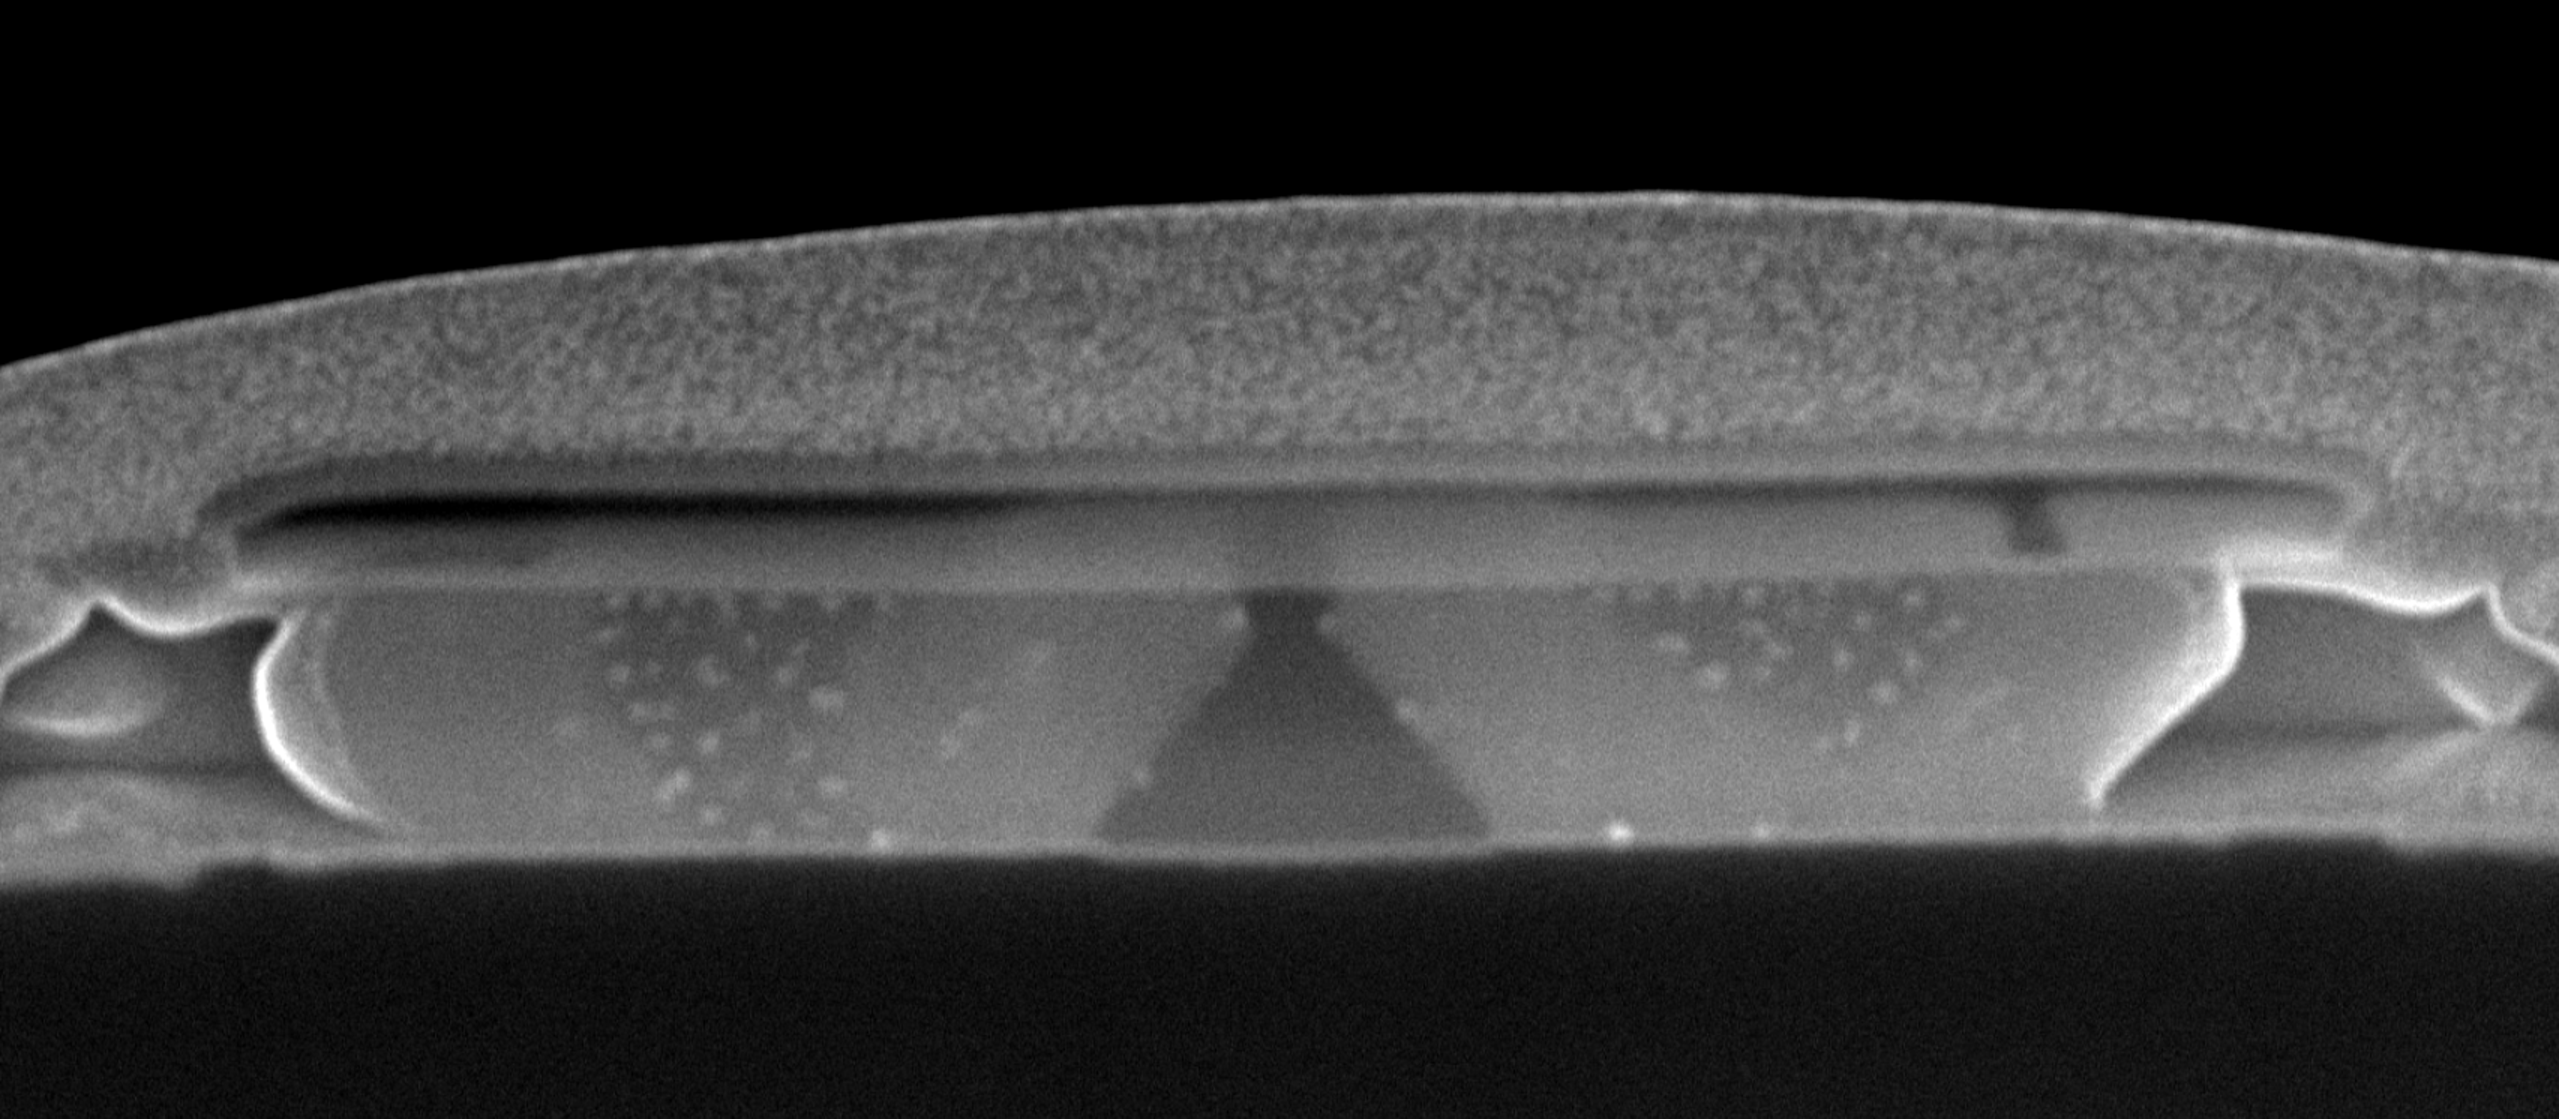
\includegraphics[width = \textwidth]{3_Growth/Sample2_FIB.pdf}};
            \node [text=white,] at (0, -2.5) {\acs{sio2}};
            \node [text=white] at (0, 0.2) {\acs{sio2}};
            \node [text=white] at (-2, -0.7) {III-V};
            \node [text=white] at (2, -0.7) {III-V};
            \node [text=white] at (0, -1.3) {\acs{si}};
            \node [text=white] at (0, 1.5) {\ce{Pt}};
            \node [text=white] at (7, -1) {Void};
            \node [text=white] at (-7, -1) {Void};
            \draw [white, |-|, very thick] (-7.2, 2.8) -- (-3, 2.8) node [midway, anchor=south] {\qty{500}{\nano\metre}};
        \end{tikzpicture}
    }
    \caption{Growth of the second sample. \subref{subfig:recipe1} Is the diagram representing the modified growth recipe introducing the looped segment for thin layer deposition \cite{Brugnolotto2023}. Each line represents an active flow of precursor into the reactor. The colour of the horizontal lines represents the target material. \subref{subfig:FIB_cut_2} \acs{sem_m} image of the lamella during \acs{fib} thinning. The various material regions are labelled.}
    \label{fig:sample2_growth}
\end{figure}

A further looped deposition segment was introduced at the end of the recipe in Figure~\ref{subfig:recipe1} to study the growth of thin structures in the template. The resulting recipe is illustrated in Figure~\ref{subfig:recipe2}. The looped segment, executed twice without interruption, contains an \acs{inp} and an \acs{ingaas} deposition step. The two short deposition steps are \qty{75}{s} long. The growth temperature was kept constant at \qty{580}{\degreeCelsius}, and the III-V ratios were unchanged from those in Table~\ref{tab:sample1_ratios}.
\par
Figure~\ref{subfig:FIB_cut_2} shows an \acs{sem_m} image of a lamella being cut from one of the T-shape devices shown in Figure~\ref{subfig:enterprise_design}. The image was taken during the last stage of \acs{fib} processing; two III-V nanowires can be observed to have grown from a central \acs{si} seed, filling the template almost entirely. The areas where the two "Void" labels are placed also mark the end of the upper template \acs{sio2} layer. The protective \ce{Pt} layer and buried oxide layers are also visible. Lamella thinning from the back side was ongoing, as the farther template wall was still present. The \acs{inp} regions for both wires are visible as being darker with brighter \acl{in} droplets.
\par
The shape of the \acs{si} seed surfaces is very similar to those of the previous samples (Figures~\ref{subfig:FIB_cut} and \ref{subfig:sample1_cross-sec}) with the upper \hkl{1 1 1} facet being the smaller of the two. This regularity in seed shape could be attributed to the fact that the templates in all three samples were opened during the same \acf{rie} run, as they were processed simultaneously until the \acs{si} etch back step right before growth. The two seed facets in Figure~\ref{subfig:FIB_cut_2} formed when the \acs{tmah} etch back of the sacrificial \acs{si} was stopped just before entering the "stem" of the T shape. 
\par
It is interesting to notice how the contrast of the III-V / upper \acs{sio2} layer contact interface is broken by a darker segment for the wire on the right. Even in correspondence of the void region seen in Figure~\ref{subfig:FIB_cut}, the interface appeared bright; this is likely due to the \ce{Pt} deposited just before \acs{fib} cutting, creating a contact interface. This darker region could result from a void formed during \acs{mocvd} growth inside the wire itself.

\subsection{\texorpdfstring{\acs{stem_m} analysis}{STEM analysis}}

\begin{figure}
    \centering
    \subcaptionbox{
        \acs{bf}-\acs{stem_m} image of the right wire of sample 2 \cite{Brugnolotto2023}.
        \label{subfig:s2_r_ov}
        }{\begin{tikzpicture}
            \node[inner sep=0pt] (image) at (0,0) {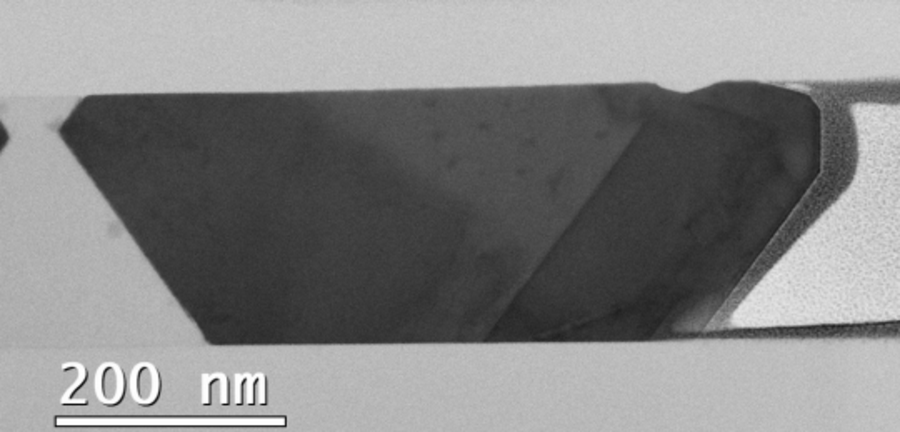
\includegraphics[width = \textwidth]{3_Growth/S2_right_overview.pdf}};
        \end{tikzpicture}
    }
    \subcaptionbox{
        \acs{eds} map: red-\acs{in}, blue-\acs{ga} \cite{Brugnolotto2023}.
        \label{subfig:s2_III_ov_EDS}
        }{\begin{tikzpicture}
            \node[inner sep=0pt] (image) at (0,0) {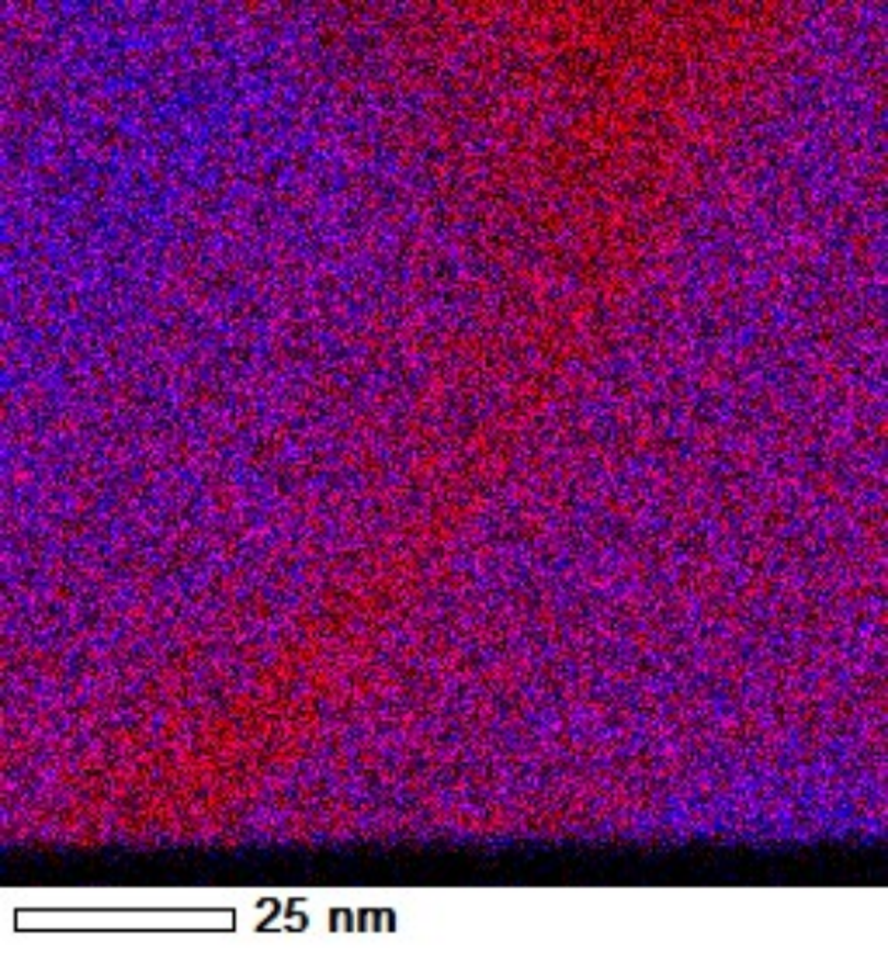
\includegraphics[width=0.45\textwidth]{3_Growth/s2_III_ov_EDS.pdf}};
        \end{tikzpicture}
    }
    \subcaptionbox{
        \acs{eds} map: red-\acs{as}, blue-\acs{p} \cite{Brugnolotto2023}.
        \label{subfig:s2_V_ov_EDS}
        }{\begin{tikzpicture}
            \node[inner sep=0pt] (image) at (0,0) {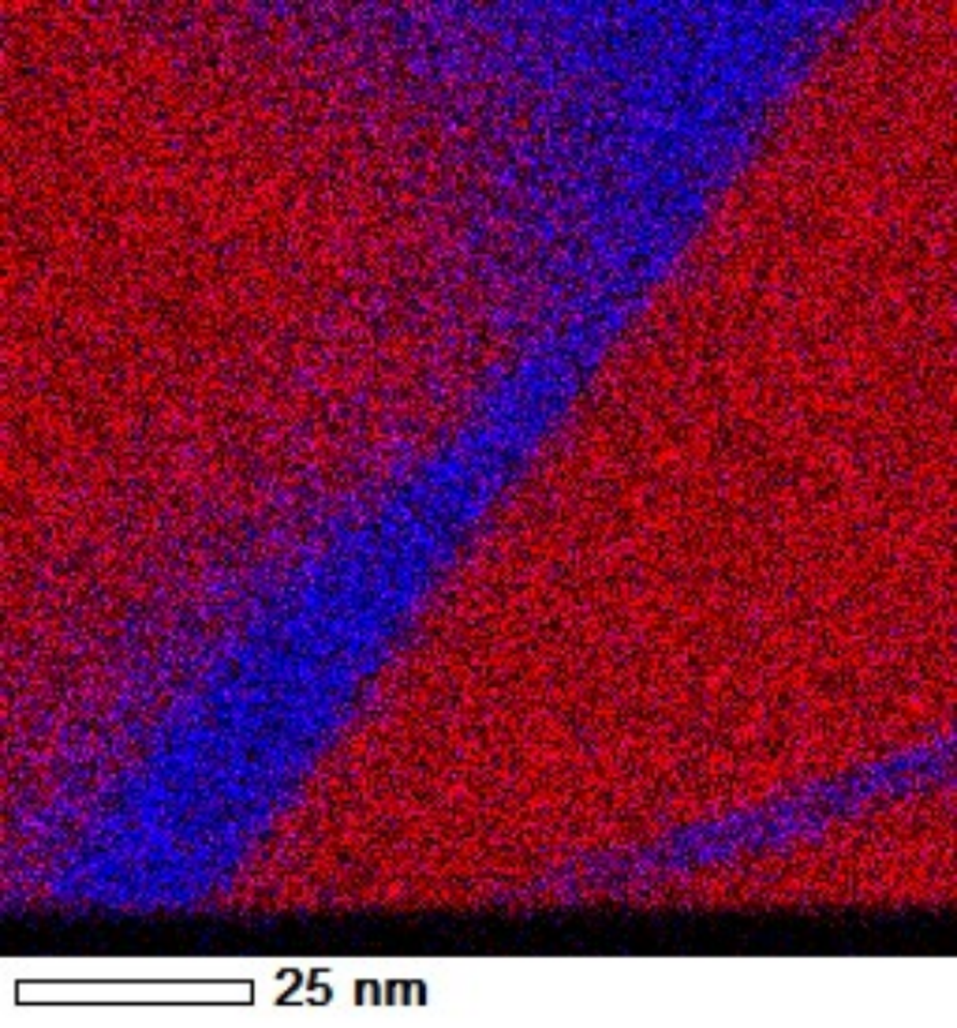
\includegraphics[width=0.45\textwidth]{3_Growth/s2_V_ov_EDS.pdf}};
        \end{tikzpicture}
    }
    \caption{Microscopy images of the second sample. \subref{subfig:s2_r_ov} Is a \acs{bf}-\acs{stem_m} image of the lamella of sample 2, centred on the right wire. Various interfaces are visible, such as the \acs{si}/III-V interface and those between the two materials in the thick \acs{inp} and \acs{ingaas} layers. Some other areas of interest are also present.}
    \label{fig:sample2_stem}
\end{figure}

The \acs{stem_m} analysis of the sample started with the recording of the overview image in Figure~\ref{subfig:s2_r_ov}. It is a \acs{bf}-\acs{stem_m} image showing the right wire visible in Figure~\ref{subfig:FIB_cut_2}. The \acs{si} seed presents the previously discussed "V"-shaped interface composed of two \hkl{1 1 1} facets, which are once more identifiable by the image contrast on the left side of the image. A brighter region within the dark III-V material segment coincides with the presence of \acs{inp}. The evolution of the interfaces follows the trend that was highlighted in sample 1, with an initial \acs{ingaas} segment growing with a multi-faceted growth front exhibiting both \hkl{1 1 0} and \hkl{1 1 1} facets. The following \acs{inp} layer grows quickly in the \hkl{1 1 0} directions, and as such, the bottom \hkl{1 1 1} facet is larger. However, in the following segment, thinner material layers can no longer be identified through channelling-driven differences in contrast.
\par
\paragraph{Facet selection} The presence of two top \hkl{1 1 0} facets and the tendency of multiple facets of this family to form in this growth configuration is also reflected in the existing literature \cite{Borg2014, Schmid2015, Borg2015, Knoedler2017}. The initial nucleation sees the formation of a multi-faceted \acs{ingaas} particle resting on the \acs{si} seed surface. As it grows, the difference in growth rates of the different facets and the template walls limit which facets establish a stable growth front. Looking at the \hkl[1 1 0] growth axis in the cubic system, there are five energy-equivalent \hkl{1 1 0} facets available, of which the first is perpendicular to the template orientation and the other four's defining vector is offset by \qty{60}{\degree} from the first one's. On the other hand, there are only two available \hkl{1 1 1} facets at \qty{35.3}{\degree} close to the template direction. Furthermore, in the zincblende system, the \hkl{1 1 1} facets can be classified as \hkl{111}\(_A\) and \hkl{111}\(_B\) depending on whether only III or V atoms are exposed, respectively. The high V/III ratio loaded into the reactor during the \acs{inp} deposition step selects the \hkl{111}\(_B\) facet due to the marked prevalence of \acl{p} in the reactor atmosphere. The same \acl{p} saturation is likely to occur on the \hkl{1 1 0} facets; however, the difference in the morphology of the facet means that growth is enhanced on this facet, leading to its annihilation.

An example of how the different growth rates for each facet family affect the shape of the crystal is seen in the \acs{ingaas} layer immediately after this central \acs{inp} region. Here, growth appears to be relatively slow on \hkl{1 1 2} facets, and at the top of the wire, a void region is created. Looking at Figure~\ref{subfig:FIB_cut_2}, this information confirms the interpretation of the darker region spotted at the top of the right wire on the upper \acs{sio2} template wall. This allows a better understanding of the shape of this void region: its limits are mainly perpendicular to the template axis, except in the area closest to the far template wall, where it appears that the limit closest to the seed curves back.
\par
\paragraph{Initial spectroscopic analysis} III and V element EDS maps centred on the central \acs{inp} segment are shown in Figure~\ref{subfig:s2_III_ov_EDS} and \ref{subfig:s2_V_ov_EDS} respectively. Once again, the thick \acs{inp} layer already identified through channelling contrast is immediately noticeable at the centre of the images. However, the V map in Figure~\ref{subfig:s2_V_ov_EDS} also shows an important clue to the location of one of the heterointerfaces in the thin layer segment at the end of the wire. A small blue line is visible on the bottom right of this image, revealing the presence of \acl{p} in this area of the wire. This phosphide layer originated from the \qty{75}{\second} long pulse in the looped segment of the recipe shown in Figure~\ref{subfig:recipe2} and is well defined, without shading at the edges, which means that the growth front facet was perpendicular to the viewing direction. Despite this, no corresponding \acs{in}-rich layer is found in Figure~\ref{subfig:s2_III_ov_EDS}. This finding points to a difference in the relationship between precursor flow and elemental incorporation during material growth for the III and the V elements when the growth occurs in templates.
\par


\begin{figure}
    \centering
    \subcaptionbox{
        High-Res \acs{bf}-\acs{stem_m} image of the \acs{inp} layer \cite{Brugnolotto2023}.
        \label{subfig:s2_thick_heterostructure}
        }{\begin{tikzpicture}
            \node[inner sep=0pt] (image) at (0,0) {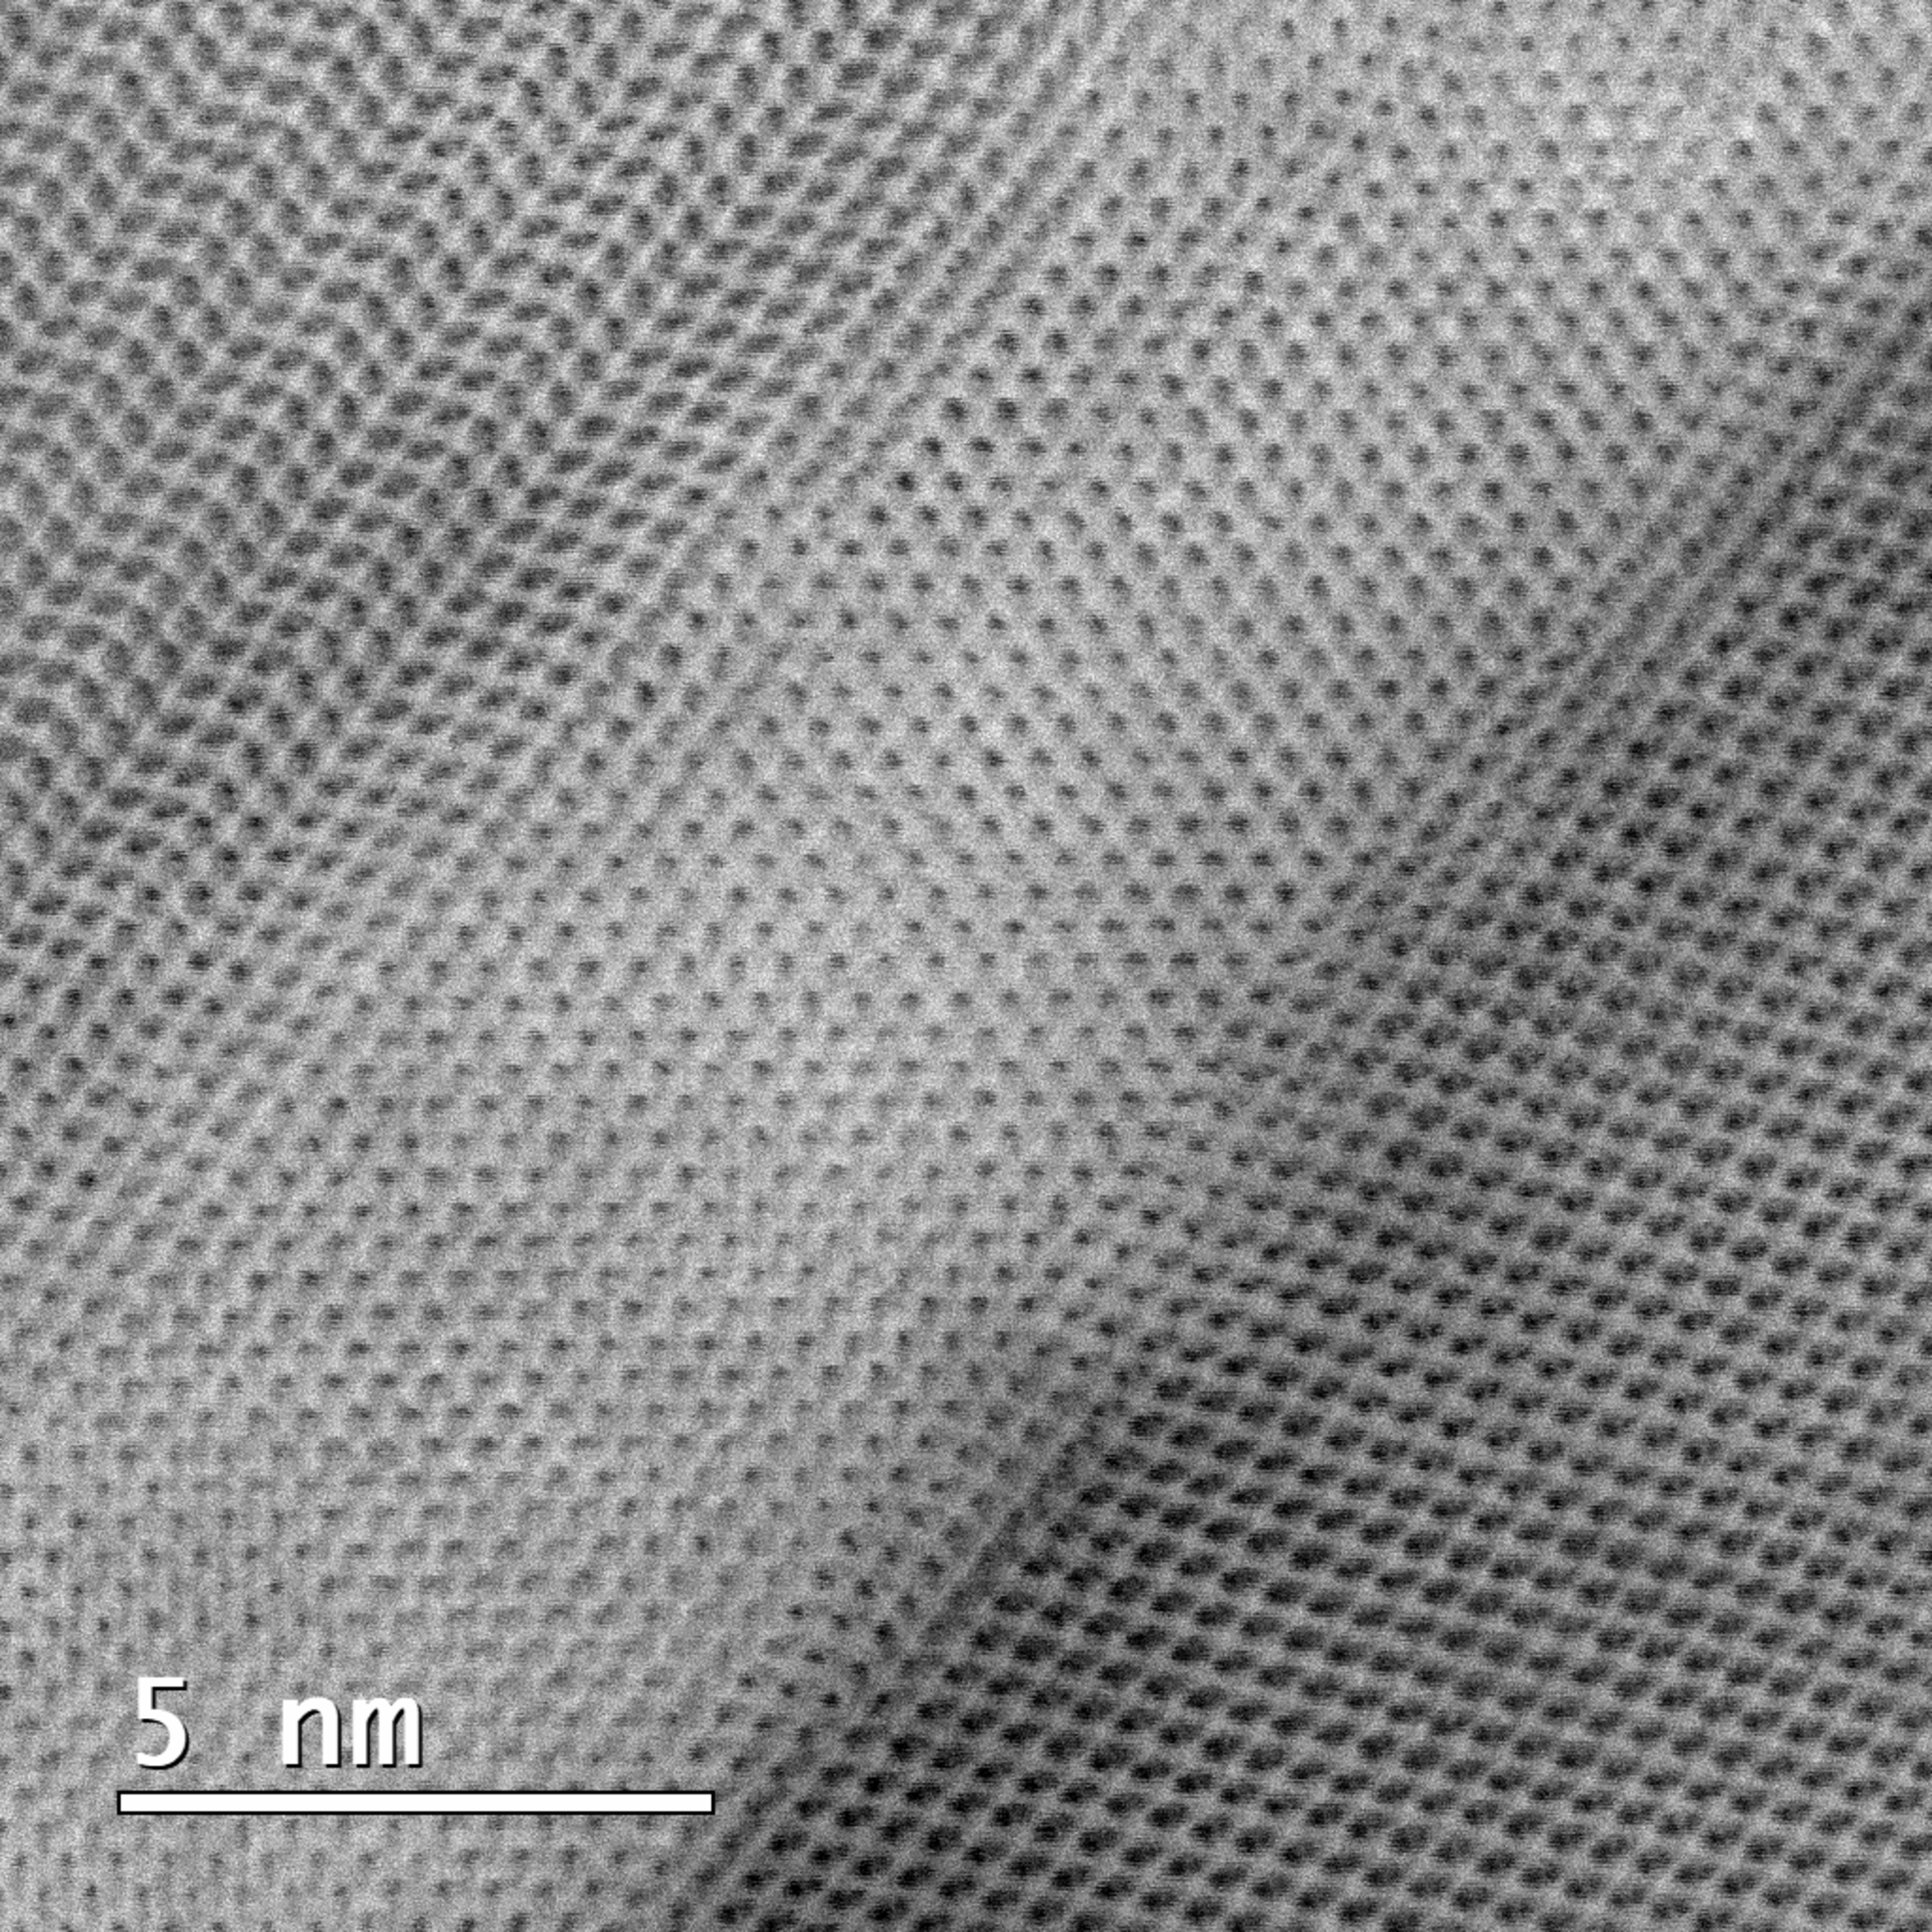
\includegraphics[width=0.45\textwidth]{3_Growth/s2_thick_Heterostructure.pdf}};
        \end{tikzpicture}
    }
    \subcaptionbox{
        High-Res \acs{bf}-\acs{stem_m} image of the III-\acs{p} layer.
        \label{subfig:s2_V_thin_heterostructure}
        }{\begin{tikzpicture}
            \node[inner sep=0pt] (image) at (0,0) {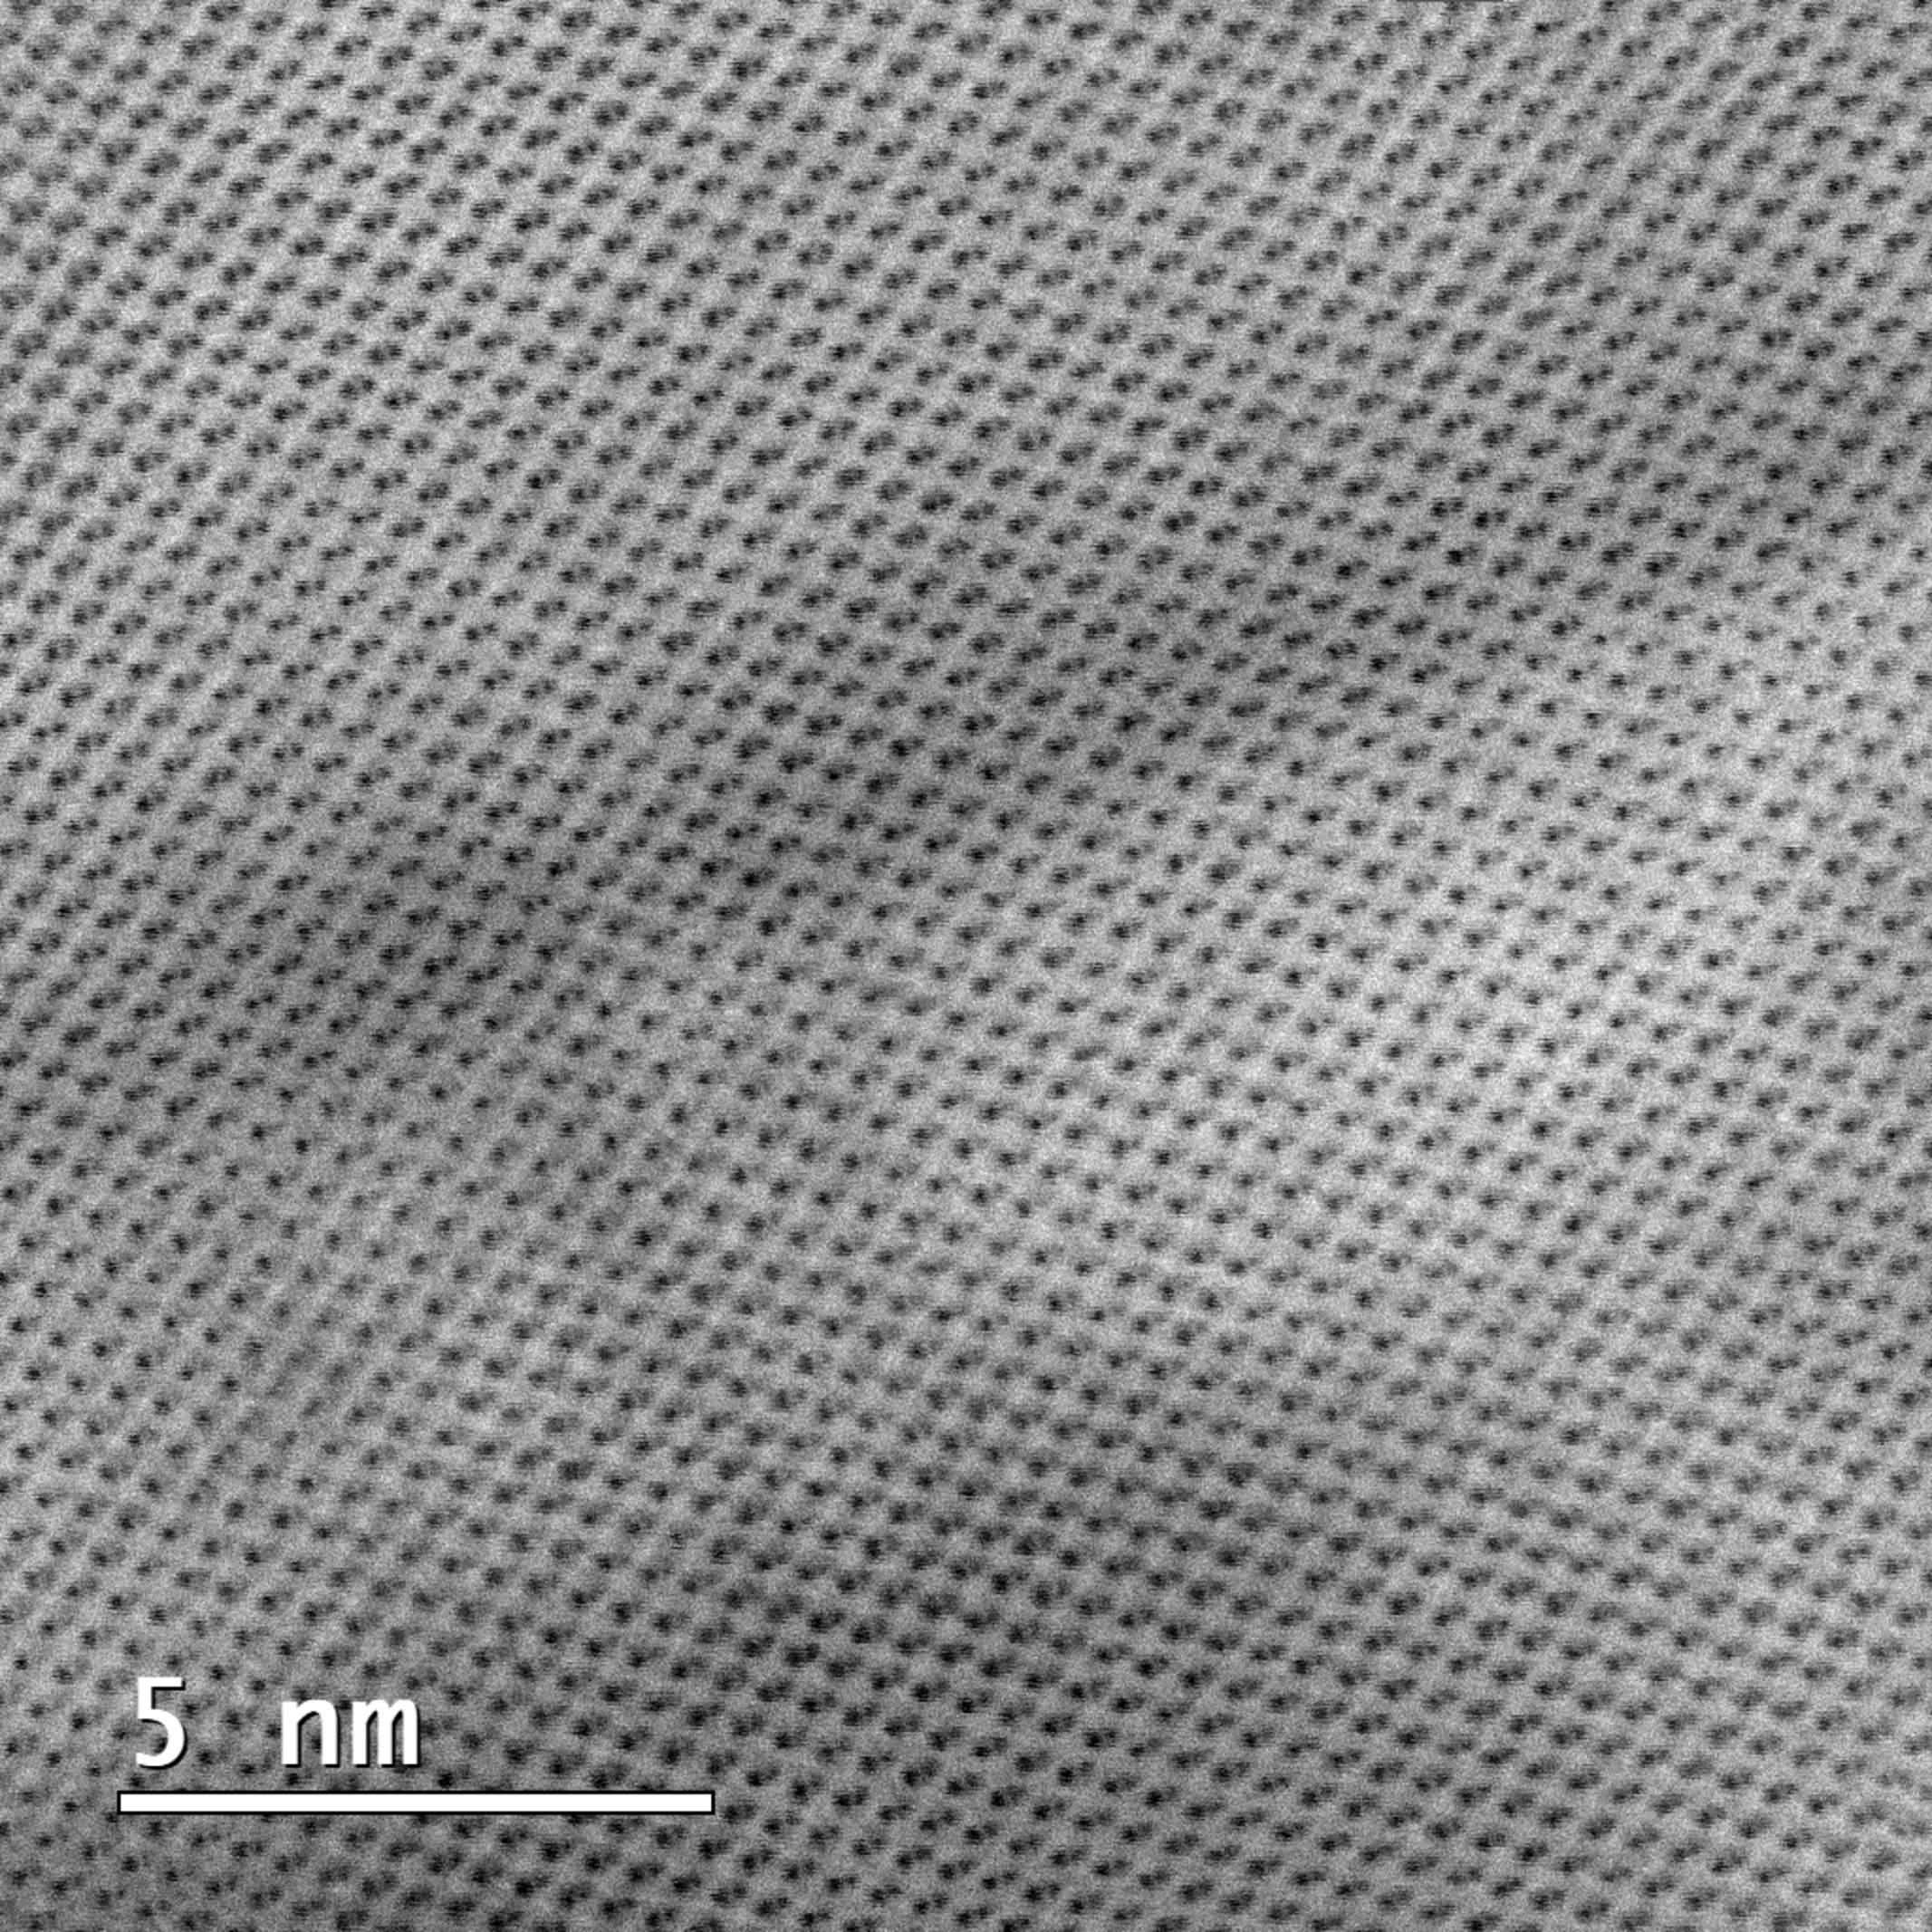
\includegraphics[width=0.45\textwidth]{3_Growth/s2_thin_Heterostructure.pdf}};
        \end{tikzpicture}
    }
    \subcaptionbox{
        \acs{eds} map of the \acs{p} concentration.
        \label{subfig:s2_int2_P}
        }{\begin{tikzpicture}
            \node[inner sep=0pt] (image) at (0,0) {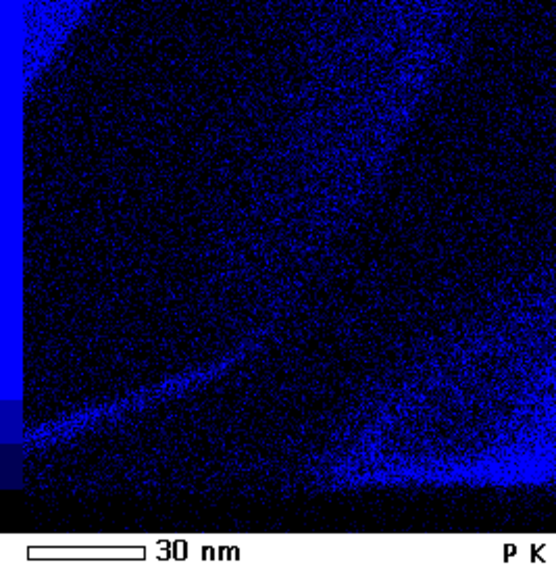
\includegraphics[width=0.45\textwidth]{3_Growth/s2_int2_P.pdf}};
        \end{tikzpicture}
    }
    \subcaptionbox{
        \acs{eds} map of the \acs{in} concentration.
        \label{subfig:s2_int2_In}
        }{\begin{tikzpicture}
            \node[inner sep=0pt] (image) at (0,0) {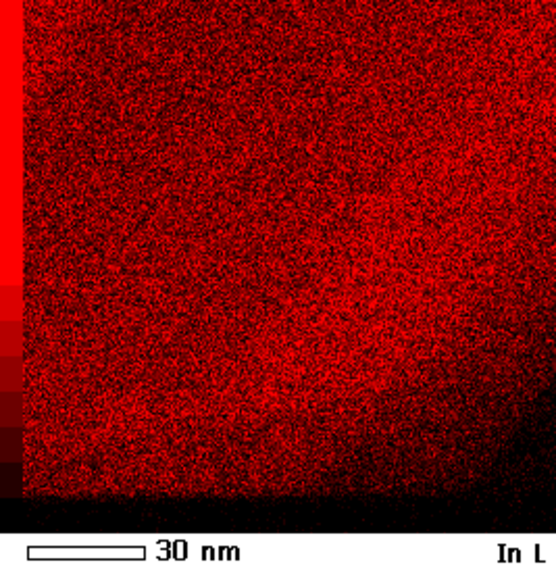
\includegraphics[width=0.45\textwidth]{3_Growth/s2_int2_In.pdf}};
        \end{tikzpicture}
    }
    \caption{Analysis of the thin-layer region. \subref{subfig:s2_thick_heterostructure} \acs{bf}-\acs{stem_m} image of the lower part of the thick \acs{inp} layer, where it is at its thinnest. \subref{subfig:s2_V_thin_heterostructure} \acs{bf}-\acs{stem_m} image of the thin phosphide interface at the bottom left of \ref{subfig:s2_r_ov}. \subref{subfig:s2_int2_P} \acs{eds} composition map of \acl{p} presence in the sample. \subref{subfig:s2_int2_In} \acs{eds} composition map of \acl{in} presence in the sample.}
    \label{fig:s2_details}
\end{figure}

\paragraph{High-resolution imaging} Two high-resolution \acs{bf}-\acs{stem_m} images of the phosphide segments identified in the spectroscopic analysis of the sample are presented in Figure~\ref{subfig:s2_thick_heterostructure} and \ref{subfig:s2_V_thin_heterostructure}. Figure~\ref{subfig:s2_thick_heterostructure} shows the layer resulting from the long \acs{inp} deposition step sandwiched between two \acs{ingaas} segments. The two materials are easily distinguishable, as the III-\acs{as} couples have similar sizes for both atoms. In contrast, the \acl{p} atoms are much smaller and are almost invisible next to the \acl{in} atoms in the \acs{inp} region. \acl{rtp}s are visible on the top left of the image, in the \acs{ingaas} layer. However, they are not visible after the \acs{inp} layer in the next \acs{ingaas} layer. This, coupled with the presence of \hkl{1 1 2} facet in the growth front, could indicate that something is affecting the growth of the wire after this point: precisely what cannot be analysed easily after the growth itself is complete. Therefore, it becomes prudent to avoid drawing conclusions about the shape of the growth front morphology after this area. However, an analysis of how the III and V composition profiles interact is still possible, as this is related to the diffusion of the precursor in the template. Further, the thickness of the phosphide layer in Figure~\ref{subfig:s2_V_thin_heterostructure} is \qty{6}{nm}, indicating the potential for thin heterostructures with well-defined composition gradients. 

\paragraph{Further spectroscopic analysis} The ending region of the wire was further analysed with \acs{eds}, resulting in the two images in Figure~\ref{subfig:s2_int2_P} and \ref{subfig:s2_int2_In}. They show the concentration profiles calculated from the signal intensity at the \acl{p} K line and \acl{in} L line, respectively. As discussed during the analysis of the previous sample, the \acl{p} K\(_\alpha\) line is very close in energy to the \ce{Pt} M line. Therefore, the high \acl{p} signal visible on the bottom right of the image is interpretable as \ce{Pt} presence. 

This comparison aims to evaluate the growth of the \acs{inp} segment based on how the \acl{in} and \acl{p} concentrations line up in the sample. As is particularly evident from observing the top right corners of each \acs{eds} map, the area with high \acl{in} concentration is to the left of the one with high \acl{p} concentration. This indicates a delay in III-element integration compared to the corresponding V-element integration step. This is likely due to a difference in diffusion between the two materials and will need to be solved if precise integration of thin III-V material layers is to be attempted.

The calculations of growth rates for this terminal area of the wire are made impossible by the complex layer morphology and, most importantly, the high composition intermixing between material layers.

\subsection{Correlation between growth dynamics and results}
Figure~\ref{fig:issues} summarises the four main findings from the first two samples, which were grown using relatively simple \acs{mocvd} recipes. The stabilisation of the \hkl{1 1 1} facet in high V/III ratio \acs{inp} deposition makes this combination of material and facet the preferred one for the growth of thin heterostructures. The potential for thin hetero layers and \acl{qw}s was highlighted by the \qty{6}{\nano\metre} wide phosphide structures shown in the second sample. The thickness of the \acs{inp} layer in Figure~\ref{subfig:s2_thick_heterostructure} can be misleading, as without the context given by the larger overview image in Figure~\ref{subfig:s2_r_ov}, the information is lost that most of the material deposition occurs on the \hkl{1 1 0} facets. 
\par
Still, both Figure~\ref{subfig:s2_thick_heterostructure} and Figure~\ref{subfig:s2_V_thin_heterostructure} show that for the V component of the semiconductor, it is possible to obtain <\qty{10}{\nano\metre} thick compositional structure. However, for the III elements, short deposition pulses lead to heavy alloying and delay in integration. This indicates the presence of different diffusion mechanisms that affect the supply of reactant to the reaction interface (the growth front). 

When the possible diffusive pathways available to the precursors are examined, it becomes clear that gas-phase diffusion is the first route available directly from the showerhead, through which precursors are introduced into the reactor. However, when the precursors land on the wafer, the surface is non-reactive, unlike in planar growth, and the adsorbed precursors either desorb and continue diffusion through the gas phase or diffuse on the surface to reach the reaction interface. If the V precursors mainly desorb from the surfaces and the majority of them get the reaction interface through gas-phase diffusion, and if the III precursors tend to diffuse as adsorbates on the surface, then this could be the diffusive mechanism difference that can explain the different sharpnesses in heterointerfaces. Additionally, if it is assumed that adsorbate diffusion is a slower mechanism than vapour phase diffusion, then this could also explain the integration delay of III elements compared to their expected layer. 

These two diffusion routes are illustrated in Figure~\ref{subfig:diffusion_mechanisms}. Given the small volume of the cavities, Knudsen vapour phase diffusion occurs inside the template. This diffusion regimen appears when the mean free path of the diffusing element is comparable to the size of the area within which it is diffusing. Simultaneously, the III-elements diffuse inside the template with the additional mechanism of adsorbate diffusion. This means that the III atoms can jump from equilibrium to equilibrium site on the surface of the template oxide until they reach the reaction interface. The effects of the different availability of these diffusion pathways to the various species are highlighted for short deposition pulses as the deposition time approaches the diffusion timescales \cite{Brugnolotto2023}.

\begin{sidewaysfigure}
    \centering
    \subcaptionbox{
    The main findings from the first two samples are represented schematically. From left to right, the stabilisation of the \hkl{1 1 1} growth front during \acs{inp} growth, the thin phosphide heterolayers, III-element composition intermixing, and the diffusion-driven integration delay are shown.
    \label{fig:issues}
    }{\begin{tikzpicture}
        \node[inner sep=0pt] (image) at (0,0) {
\includegraphics[width=0.45\textwidth]{3_Growth/issues.pdf}};
    \end{tikzpicture}
    }
    \subcaptionbox{
    Diffusion mechanisms inside the \acs{sio2} interface. Bulk materials are labelled, with the two \acs{sio2} template layers above and below the III-V wire. The precursors are represented by black (III-element precursors) and grey (V-element precursors) circles. \cite{Brugnolotto2023}.
    \label{subfig:diffusion_mechanisms}
    }{
        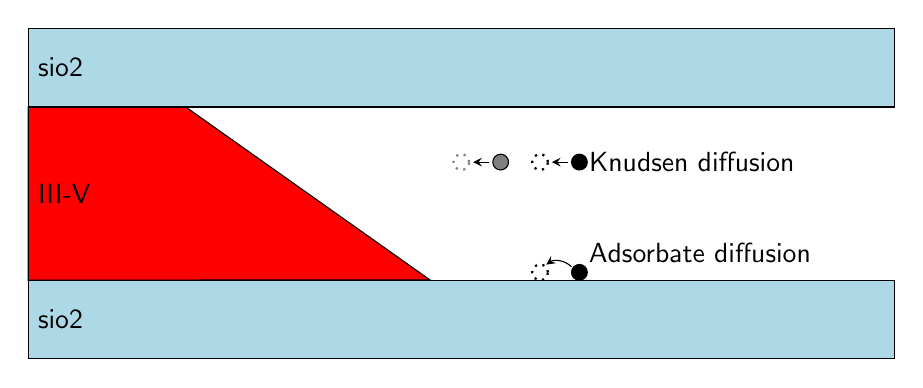
\begin{tikzpicture}
            \filldraw[fill=red] (0cm, 0cm) -- node[midway, anchor = west] {III-V} (0cm, 22mm) -- (2cm, 22mm) -- ++ (-35.3:3.8cm) --  cycle;
            \filldraw[fill=SiO2_blue] (0cm, -10mm) -- (11cm, -10mm) -- (11cm, 0cm) -- (0cm, 0mm) --  node[midway, anchor=west] {\acs{sio2}} cycle;
            \filldraw[fill=SiO2_blue] (0cm, 22mm) -- (11cm, 22mm) -- (11cm, 32mm) -- (0cm, 32mm) --  node[midway, anchor=west] {\acs{sio2}} cycle; 
            \filldraw[fill=black] (7, 1.5) circle (1mm) node [anchor = west] {Knudsen diffusion};
            \draw[-stealth] (6.85, 1.5) -- (6.65, 1.5);
            \draw[dotted, thick] (6.5, 1.5) circle (1mm);
            \filldraw[fill=gray] (6, 1.5) circle (1mm);
            \draw[-stealth] (5.85, 1.5) -- (5.65, 1.5);
            \draw[gray, dotted, thick] (5.5, 1.5) circle (1mm);
            \filldraw[fill=black] (7, 0.1) circle (1mm) node [anchor = south west] {Adsorbate diffusion};
            \draw[-stealth] (6.9, 0.17) arc[start angle = 45, end angle = 125, radius = 0.25];
            %\draw[-stealth] (6.85, 0.1) -- (6.65, 0.1);
            \draw[dotted, thick] (6.5, 0.1) circle (1mm);
            %\draw (3.2cm, 22mm) arc [start angle = 180, end angle = 324.7, radius = 3mm] node[midway, anchor = north east]{\qty{144.7}{\degree}};
            %\draw[-stealth] (8cm, 7mm) node[anchor=north] {\hkl<1 -1 0>} -- ++ (90:0.8cm) node[anchor=south] {\hkl<0 0 1>};
            %\draw[-stealth] (8cm, 7mm) -- ++ (0:0.8cm) node[anchor=west] {\hkl<1 1 0>};
            %\node[mark size=2pt] at (8, 7mm) {\pgfuseplotmark{diamond*}};
        \end{tikzpicture}
    }
    \subcaptionbox{
    Growth recipe for sample 3 \cite{Brugnolotto2023}. Each line represents an active flow of the corresponding precursor into the reactor. The colour of the horizontal lines represents the target material.
    \label{subfig:recipe3}
    }{
    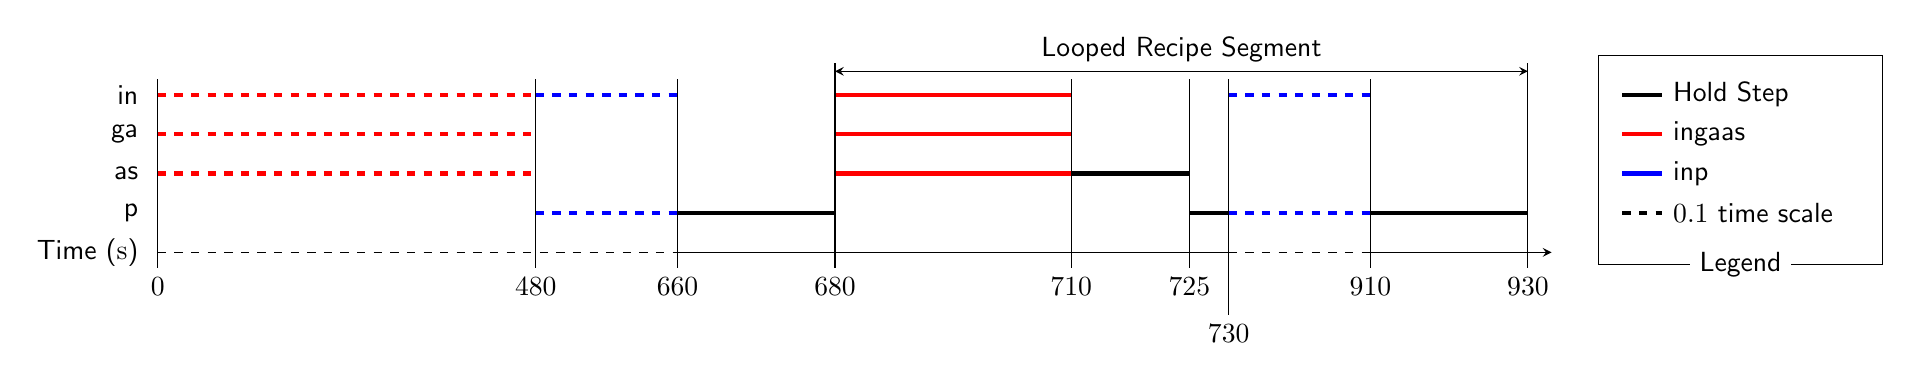
\begin{tikzpicture}
    \begin{scope}
    % lines
        \node [label={[label distance=0]180:\acs{in}}] at (0, 0) {};
        \draw [red, ultra thick, dashed] (0, 0) -- (4.8, 0); %/10
        \draw [blue, ultra thick, dashed] (4.8, 0) -- (6.6, 0); %10
        \draw [red, ultra thick] (8.6, 0) -- (11.6, 0);
        \draw [blue, ultra thick, dashed] (13.6, 0) -- (15.4, 0); %10
        %\draw [red, ultra thick] (7.35, 0) -- (8.1, 0);
        
        \node [label={[label distance=0]180:\acs{ga}}] at (0, -0.5) {};
        \draw [red, ultra thick, dashed] (0, -0.5) -- (4.8, -0.5cm); %/10
        \draw [red, ultra thick] (8.6, -0.5) -- (11.6, -0.5);
        
        \node [label={[label distance=0]180:\acs{as}}] at (0, -1) {};
        \draw [red, ultra thick, dashed] (0, -1) -- (4.8, -1); %/10
        \draw [red, ultra thick] (8.6, -1) -- (11.6, -1);
        \draw [ultra thick] (11.6, -1) -- (13.1, -1);
        
        \node [label={[label distance=0]180:\acs{p}}] at (0, -1.5) {};
        \draw [blue, ultra thick, dashed] (4.8, -1.5) -- (6.6, -1.5); %/10
        \draw [ultra thick] (6.6, -1.5) -- (8.6, -1.5);
        \draw [ultra thick] (13.1, -1.5) -- (13.6, -1.5);
        \draw [blue, ultra thick, dashed] (13.6, -1.5) -- (15.4, -1.5); %/10
        \draw [ultra thick] (15.4, -1.5) -- (17.4, -1.5);
        
    % labels and markers for the timescale
        \node [label={[label distance=0]180:Time (\second)}] at (0, -2) {};
        \draw [dashed] (0, -2) -- (6.6, -2);
        \draw [] (6.6, -2) -- (13.6, -2);
        \draw [dashed] (13.6, -2) -- (15.4, -2);
        \draw [-stealth] (15.4, -2) -- (17.7, -2);
        \draw [] (0, 0.2) -- (0, -2.2) node[anchor = north] {\num{0}};
        \draw [] (4.8, 0.2) -- (4.8, -2.2) node[anchor = north] {\num{480}};
        \draw [] (6.6, 0.2) -- (6.6, -2.2) node[anchor = north] {\num{660}};
        \draw [] (8.6, 0.4) -- (8.6, -2.2) node[anchor = north] {\num{680}};
        \draw [] (11.6, 0.2) -- (11.6, -2.2) node[anchor = north] {\num{710}};
        \draw [] (13.1, 0.2) -- (13.1, -2.2) node[anchor = north] {\num{725}};
        \draw [] (13.6, 0.2) -- (13.6, -2.8) node[anchor = north] {\num{730}};
        \draw [] (15.4, 0.2) -- (15.4, -2.2) node[anchor = north] {\num{910}};
        \draw [] (17.4, 0.4) -- (17.4, -2.2) node[anchor = north] {\num{930}};
        \draw [stealth - stealth] (8.6, 0.3) -- (17.4, 0.3) node[midway, anchor=south] {Looped Recipe Segment};
    \end{scope}
    \begin{scope} [shift={(18.6cm, -0.5)}]
        \draw [ultra thick] (0, 0.5) -- (0.5, 0.5) node[anchor = west, text=black] {Hold Step};
        \draw [red, ultra thick] (0, 0) -- (0.5, 0) node[anchor = west, text=black] {\acs{ingaas}};
        \draw [blue, ultra thick] (0, -0.5) -- (0.5, -0.5) node[anchor = west, text = black] {\acs{inp}};
        \draw [dashed, ultra thick] (0, -1) -- (0.5, -1) node[anchor = west, text = black] {\num{0.1} time scale};
        \draw (-0.3, 1) -- (3.3, 1) -- (3.3, -1.65) -- node[midway, fill = white] {Legend} (-0.3, -1.65) -- cycle;
    \end{scope}
    \end{tikzpicture}
    }
    \caption{\subref{fig:issues} Summary of insight from the first two growth runs. \subref{subfig:diffusion_mechanisms} Schematic representation of the diffusion avenues available inside the \acs{tase} template. \subref{subfig:recipe3} Modified \acs{mocvd} recipe based on the analysis of growth results.}
    \label{fig:s3_hold_steps}
\end{sidewaysfigure}

\section{Implementation of a revised switching sequence}
To address the issues identified in Figure~\ref{fig:issues}, several modifications were made to the \acs{mocvd} growth recipe, resulting in the revised step sequence shown in Figure~\ref{subfig:recipe3}. In this graphic, the segments drawn with dashed lines are represented with a \num{0.1} time scale to maintain a reasonable size for the picture. The main additions to the recipe are the "hold steps": moments at the end of each layer deposition segment when the flow of III precursors was halted, leaving only a V-element atmosphere in the background. The \qty{5}{s}-long \acl{p} hold step was introduced after the \acl{as} hold step and the \acs{ingaas} deposition step in the looped recipe segment to promote a change in the atmosphere inside the template for the following \acs{inp} deposition step. The rationale for its introduction here but not in the previous arsenide-to-phosphide step is that the smaller size and weight of the \acl{p} atom would give it a higher mobility and a lower chance to diffuse as an adsorbate compared to the bulkier, heavier \acl{as} atom. 

A second modification affected the length of the material deposition segments, which was adjusted to consider the lower growth rate of \acs{inp} compared with \acs{ingaas}. As the looped segment was repeated twice for the next growth run, this recipe will theoretically result in the correct barrier/well material layers alternating to create two \acs{ingaas} \acl{qw}s in series in a \acs{inp} matrix. The V/III ratios and the \qty{580}{\degreeCelsius} growth temperature are kept constant to continue to benefit from the stabilisation of the single \hkl{1 1 1} facet growth front that occurs during \acs{inp} deposition.

The \acs{sem_m} image of the sample during \acs{fib} processing for \acs{stem_m} analysis was already shown in Figure~\ref{subfig:FIB_cut}. A hint of the finer structure is already visible by tracking the position of the \acl{in} droplets on the exposed \acs{inp} lateral surfaces.

\subsection{\texorpdfstring{\acs{stem_m} analysis}{STEM analysis}}

\begin{figure}
    \centering
    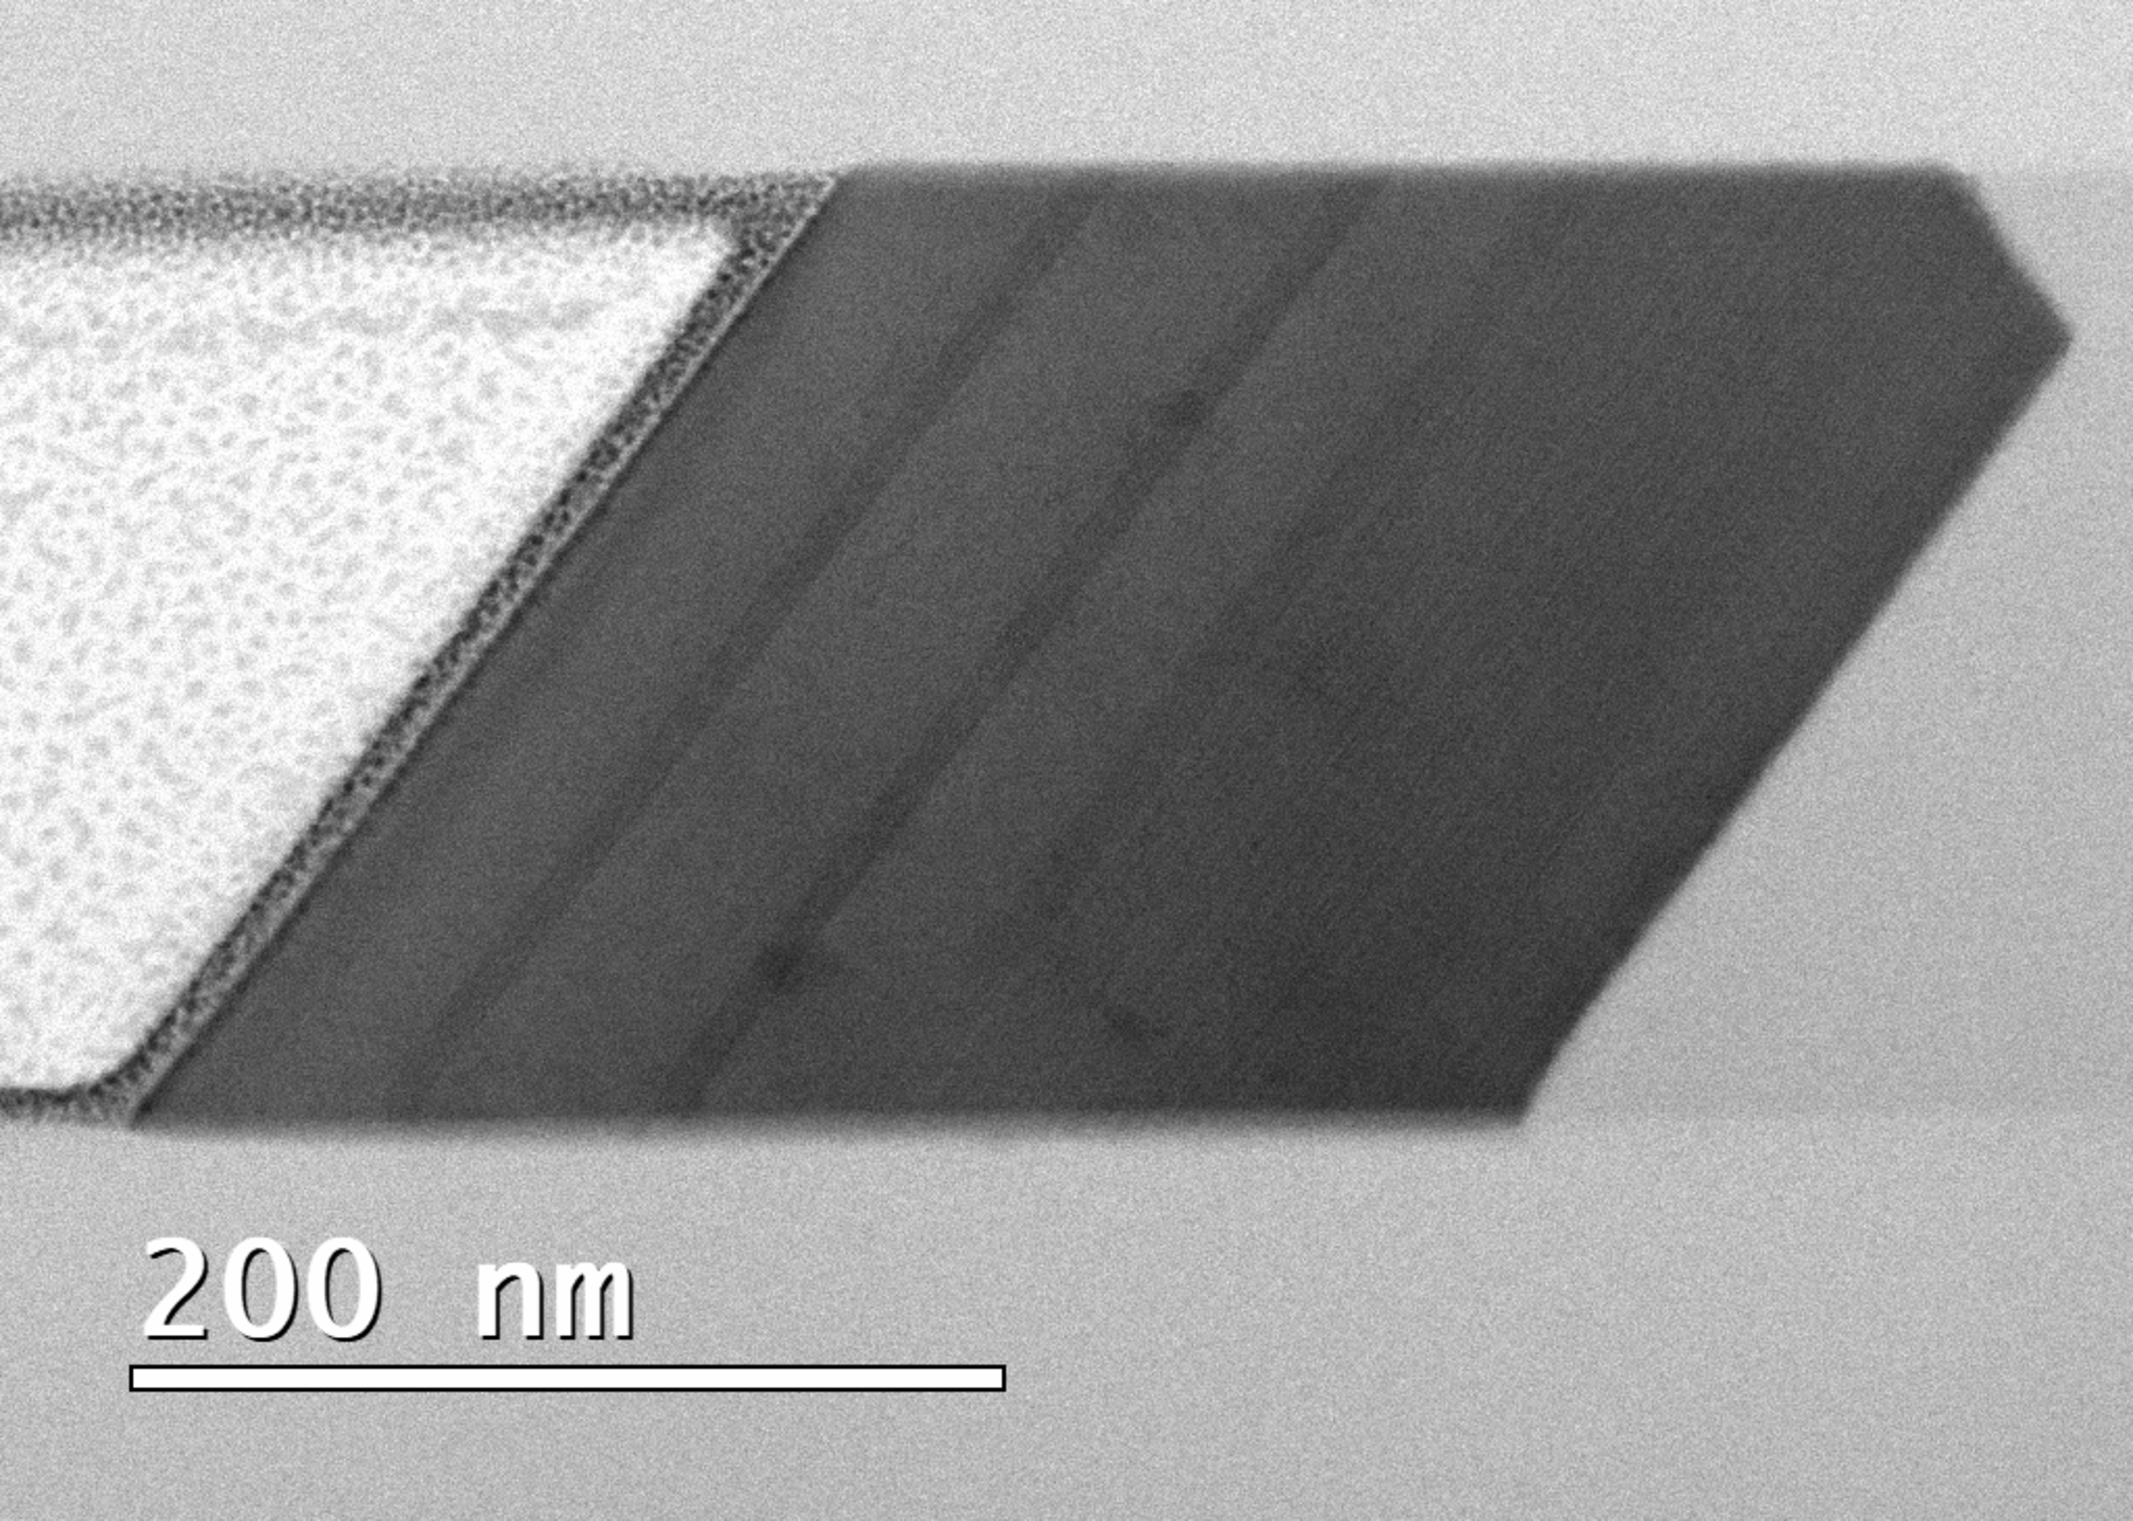
\includegraphics[width=\textwidth]{3_Growth/s3_ov.pdf}
    \caption{\acs{bf}-\acs{stem_m} image of a semiconductor lamella cut from a nanowire in sample 3 \cite{Brugnolotto2023}. Already, through channelling contrast, the different material layers are visible.}
    \label{fig:s3_ov}
\end{figure}

The \acs{bf}-\acs{stem_m} image in Figure~\ref{fig:s3_ov} gives a better view of the material layers. The wire grew right-to-left from the \acs{si} seed on the right of the image, which, once again, has the "V" shaped morphology observed in the two previous samples. Then, from right to left, the first dark area consists of an \acs{ingaas} layer, followed by a lighter \acs{inp} layer and then by an alternating \acs{ingaas} and \acs{inp} well-barrier \acl{qw} structure. Compared to sample 2 (Figure~\ref{subfig:s2_r_ov}), here the thin heterolayers are immediately visible before \acs{eds} mapping, directly from the \acs{bf}-\acs{stem_m} image.

\ce{Pt} is visible in the opening to the left of the III-V wire. The top and bottom of the image are occupied by the upper and lower \acs{sio2} template and buried oxide layers, respectively. The first \acs{ingaas} layer presents a multi-faceted growth front once again, with an upper \hkl{1 1 1} facet and a \hkl{1 1 0} region at the bottom. The following \acs{inp} layer stabilises the \hkl{1 1 1} facet up to the last few nanometres at the bottom of the wire, where a small \hkl{1 1 0} facet survives, maintained through the next \acs{ingaas} layer which is, importantly, conformal to the previous \acs{inp} segment when it comes to the morphology of the growth front. It is only in the second \acs{inp} layer that a single \hkl{1 1 1} facet is stabilised. However, it is clear that, given a sufficiently thick \acs{inp} layer, growth front stabilisation will occur.

\begin{figure}
    \centering
    \begin{tikzpicture}
        \node[inner sep=0pt] (image) at (0,0) {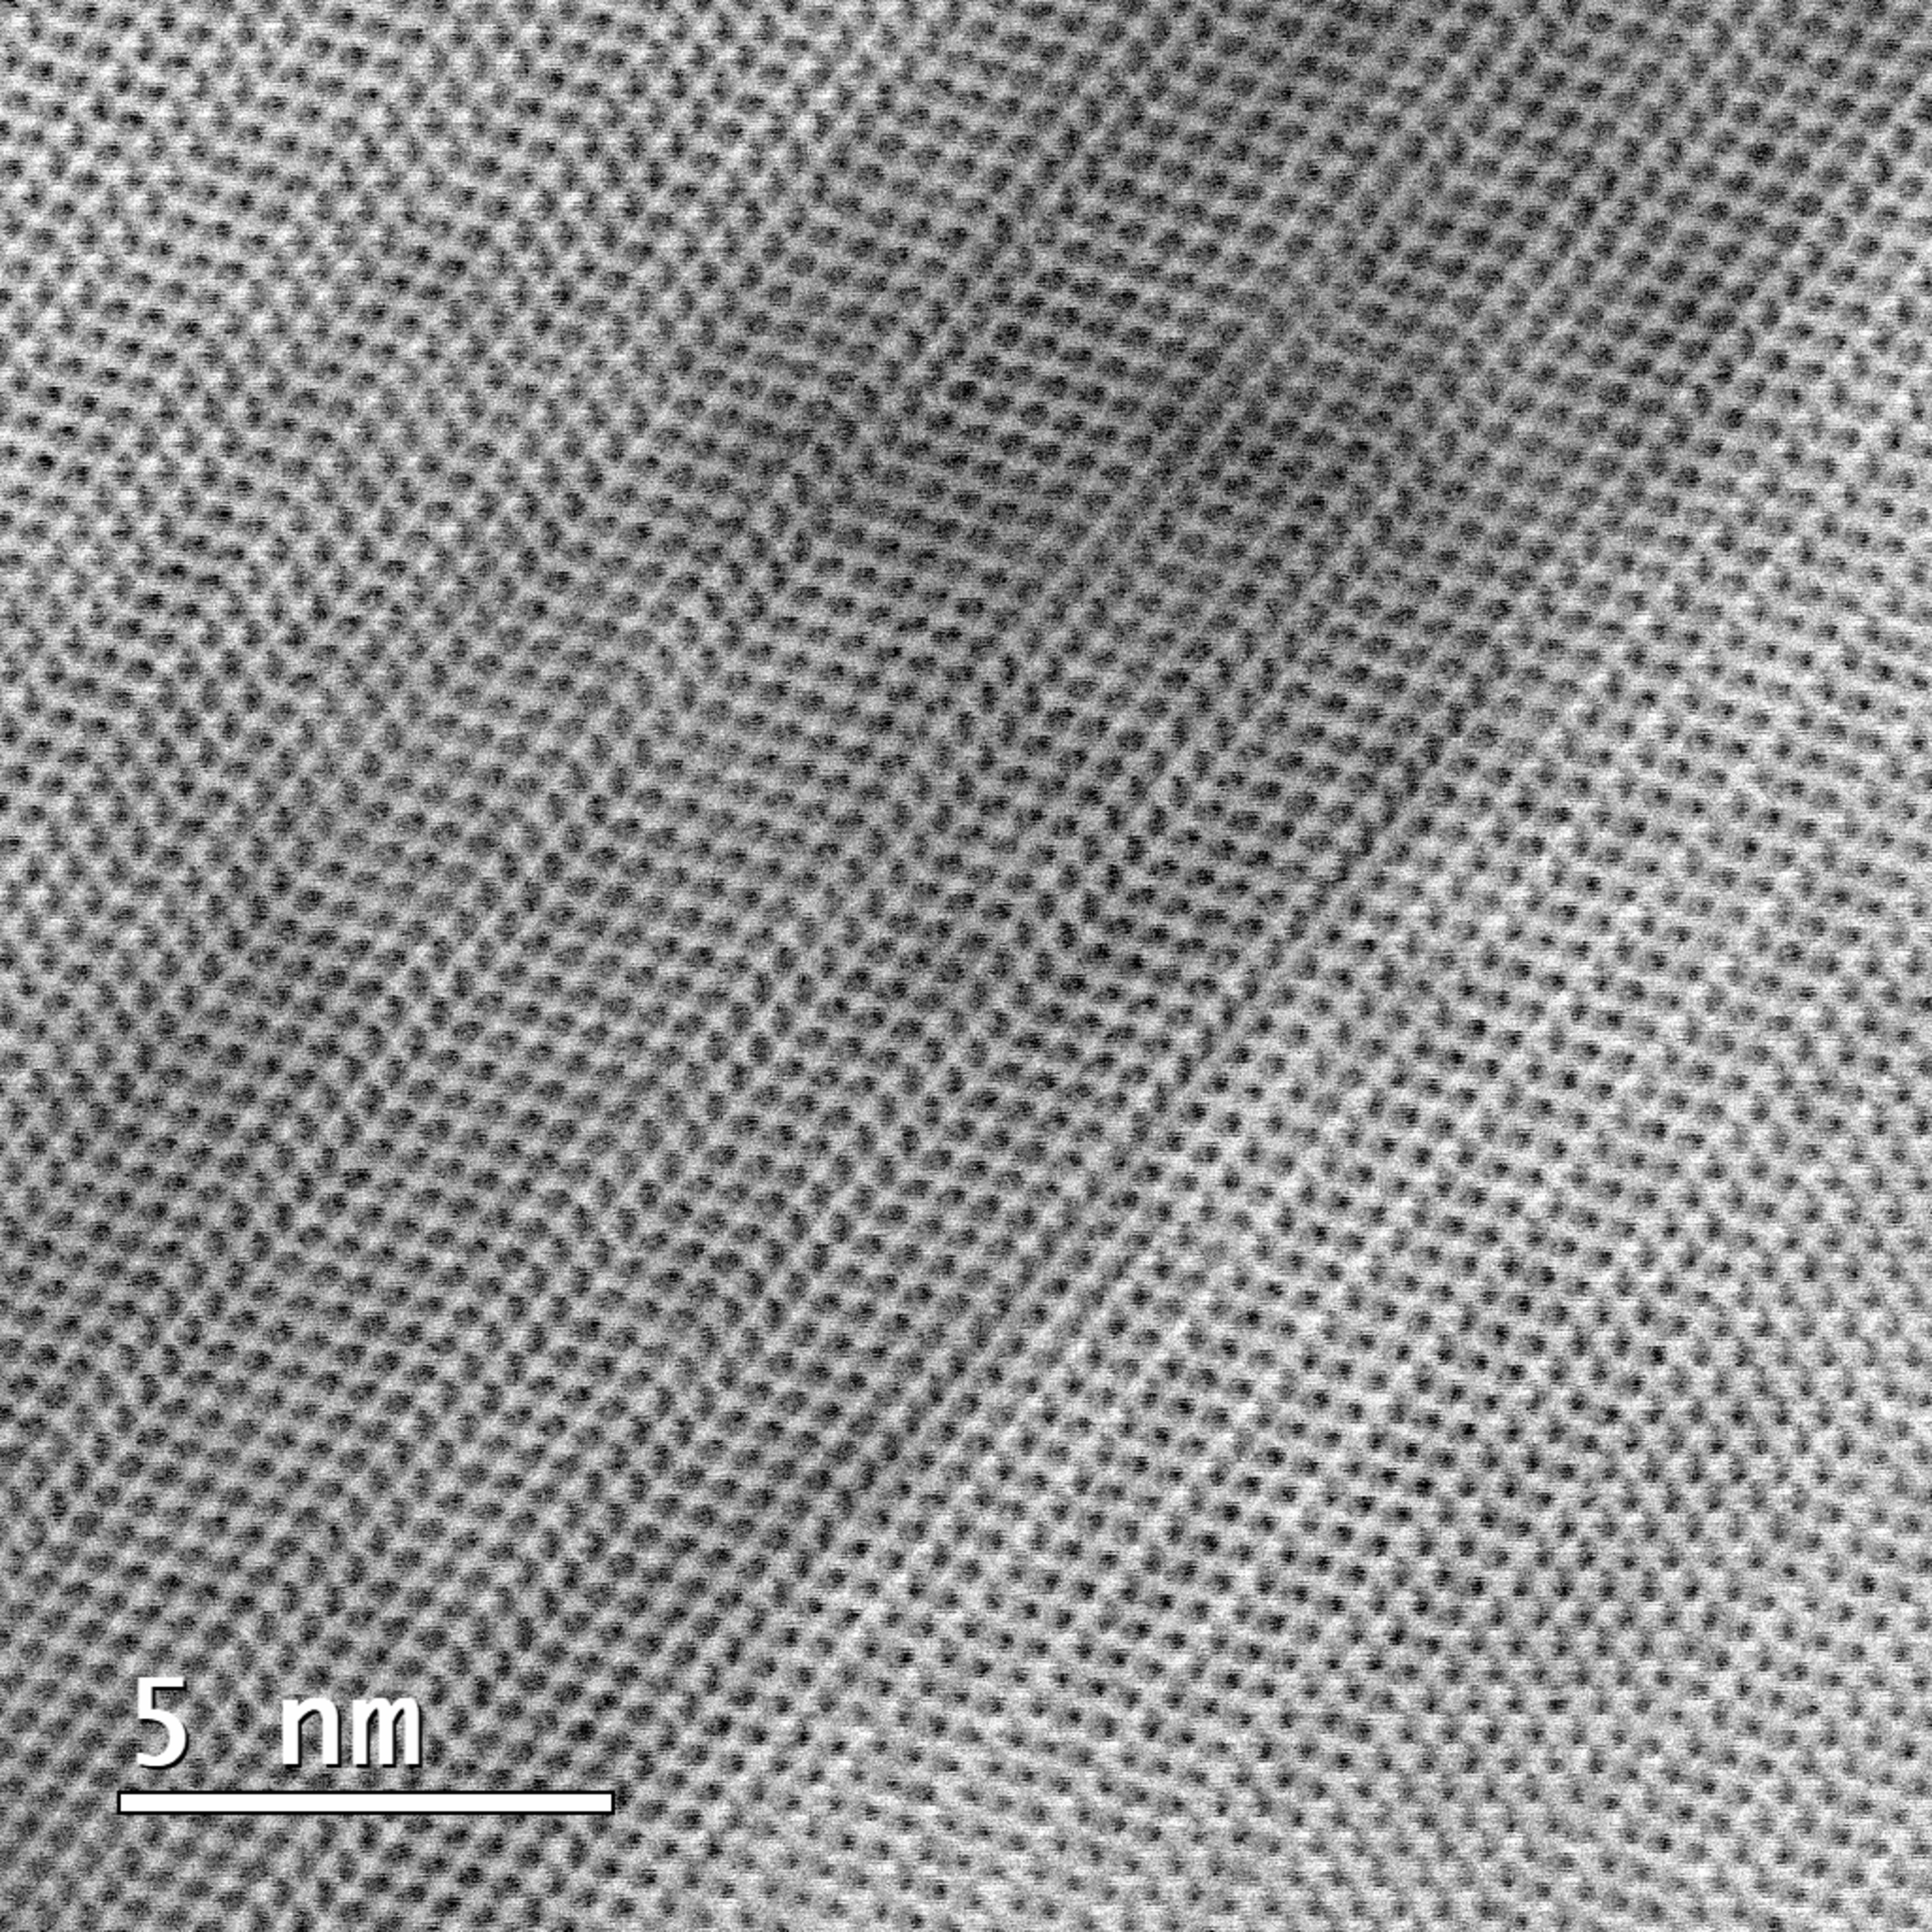
\includegraphics[width=0.5\textwidth]{3_Growth/s3_QW_HR.pdf}};
    \end{tikzpicture}
    \caption{High-resolution \acs{bf}-\acs{stem_m} image of the second \acl{qw} region of sample 3.}
    \label{fig:s3_QW_HR}
\end{figure}

\paragraph{High-resolution imaging} Lines parallel to the large \hkl{1 1 1} seed facet are already visible in the overview image in Figure~\ref{fig:s3_ov}. These are the \acl{rtp}s already discussed in previous samples and are more easily identified in the high-resolution images in Figure~\ref{fig:s3_QW_HR}, which shows the second \acl{qw} (counting from the seed, therefore from right to left) of sample 3 (Figure~\ref{fig:s3_ov}. Once more, the size difference between the \acl{p} and \acl{as} atoms creates the contrast in the image, and the arsenide layer appears darker.
\par

\begin{figure}
    \centering
    \subcaptionbox{
    \acs{eds} map: Red-\acs{in} Green-\acs{si} Blue-\acs{ga}
    \label{subfig:s3_III_map}
    }{\begin{tikzpicture}
        \node[inner sep=0pt] (image) at (0,0) {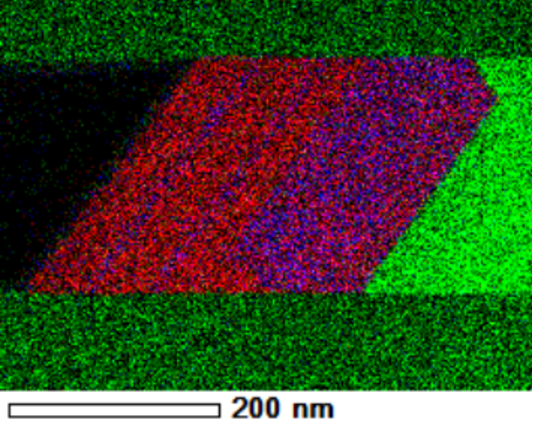
\includegraphics[width=0.45\textwidth]{3_Growth/s3_III_map.pdf}};
    \end{tikzpicture}
    }
    \subcaptionbox{
    \acs{eds} map: Red-\acs{as} Green-\ce{O} Blue-\acs{p}
    \label{subfig:s3_V_map}
    }{\begin{tikzpicture}
        \node[inner sep=0pt] (image) at (0,0) {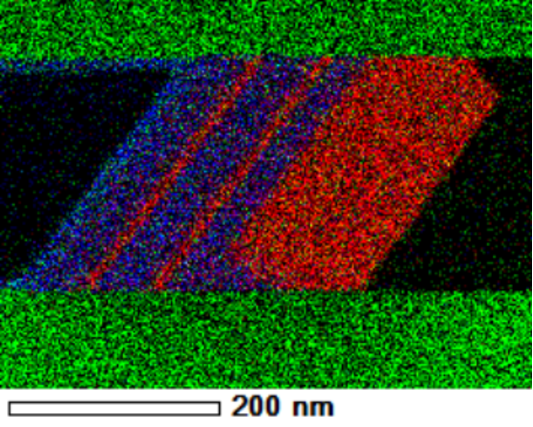
\includegraphics[width=0.45\textwidth]{3_Growth/s3_V_map.pdf}};
    \end{tikzpicture}
    }
    \subcaptionbox{
    \acs{eds} map: Red-\acs{in} Blue-\acs{ga} \cite{Brugnolotto2023}
    \label{subfig:s3_III_map_wells}
    }{\begin{tikzpicture}
        \node[inner sep=0pt] (image) at (0,0) {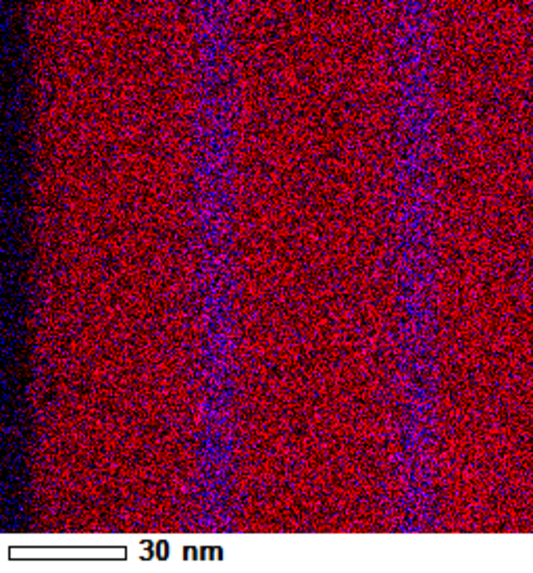
\includegraphics[width=0.45\textwidth]{3_Growth/s3_III_map_wells.pdf}};
    \end{tikzpicture}
    }
    \subcaptionbox{
    \acs{eds} map: Red-\acs{as} Blue-\acs{p} \cite{Brugnolotto2023}
    \label{subfig:s3_V_map_wells}
    }{\begin{tikzpicture}
        \node[inner sep=0pt] (image) at (0,0) {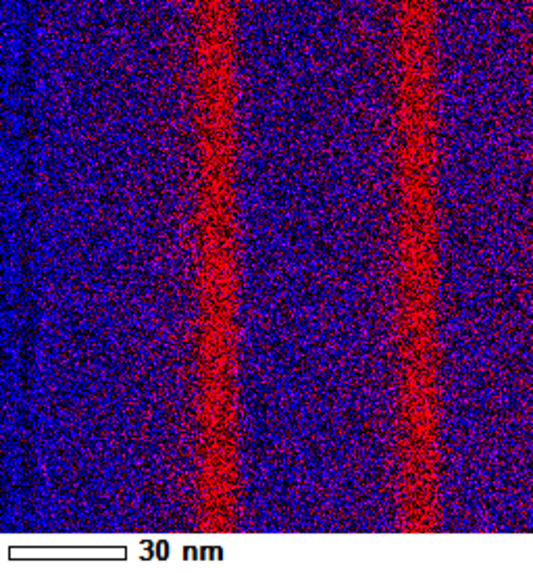
\includegraphics[width=0.45\textwidth]{3_Growth/s3_V_map_wells.pdf}};
    \end{tikzpicture}
    }
    \caption{Spectroscopic information for sample 3. \subref{subfig:s3_III_map} and \subref{subfig:s3_V_map} are the III and V element maps, with \acs{si} and \ce{O} to visualise the position of the seed and template. \subref{subfig:s3_III_map_wells} and \subref{subfig:s3_V_map_wells} are III and V \acs{eds} maps focussing on the superlattice region of the sample.}
    \label{fig:s3_maps}
\end{figure}

\paragraph{Spectroscopic analysis} The identification of the different material layers through channelling contrast is confirmed by the \acs{eds} maps in Figures~\ref{subfig:s3_III_map} and \ref{subfig:s3_V_map}, which provide spectroscopic data and composition information for the \acs{bf}-\acs{stem_m} image in Figure~\ref{fig:s3_ov}. Figure~\ref{subfig:s3_III_map}, showing the \acl{in}, \acl{si}, and \acl{ga} distribution in the sample, compared to Figure~\ref{subfig:s3_V_map}, which shows the distribution \acl{as}, oxygen, and \acl{p} distribution in the sample, demonstrate how the composition gradients for the III and V components of the sample now match each other. This proves the efficacy of hold steps in preventing intermixing between the two III-V materials.

While providing a good overview of the sample composition, these two colour-coded maps lack information on the \acl{qw}s area. Therefore, the higher resolution \acs{eds} maps in Figures~\ref{subfig:s3_III_map_wells} and \ref{subfig:s3_V_map_wells} were recorded. The scanning angle of the \acs{stem_m} was changed to show the heterostructures going from top to bottom without tilt, while keeping the growth orientation from left to right. The noticeable difference in the presence of blue "\acl{p}" signal on the left side of Figure~\ref{subfig:s3_V_map_wells} in an area where there is no III component in the corresponding map can be explained once again by the \acl{p} K\(_\alpha\) line being close in energy to the \ce{Pt} M line. 

The arsenide layers in the V map are confirmed to perfectly coincide with the \acs{ga}-rich regions. However, the V map also highlights an asymmetry in the composition of the areas immediately before and after an \acs{ingaas} quantum well, with the \acs{inp} region after a well showing a higher \acl{as} signal than the \acs{inp} region immediately before.

\begin{figure}
    \centering
    \subcaptionbox{
    \acs{eds} linescan: III atomic percentage vs position \cite{Brugnolotto2023}.
    \label{subfig:s3_III_linesc}
    }{\begin{tikzpicture}
        \begin{axis}[
            width = 0.8\textwidth,
            height = 5cm,
            xlabel = Position (nm),
            ylabel = Composition (atomic \%),
            table/col sep=comma,
            %title = III element composition,
            legend pos=outer north east,
            ymin=0, ymax=100,
            xmin = 0, xmax=20.81
        ]
    \addplot [cb1_orange,] table[x=nm,y=Ga] {3_Growth/s3_III_linesc.csv};
    \addplot [cb1_dark_blue,] table[x=nm,y=In] {3_Growth/s3_III_linesc.csv};
    \addlegendentry{Ga}
    \addlegendentry{In}
    \end{axis}

    \end{tikzpicture}
    }
    \subcaptionbox{
    \acs{eds} linescan: V atomic percentage vs position \cite{Brugnolotto2023}.
    \label{subfig:s3_V_linesc}
    }{\begin{tikzpicture}
        \begin{axis}[
            width = 0.8\textwidth,
            height = 5cm,
            xlabel = Position (nm),
            ylabel = Composition (atomic \%),
            table/col sep=comma,
            %title = V element composition,
            legend pos=outer north east,
            ymin=0, ymax=100,
            xmin = 0, xmax=20.81
        ]
    \addplot [cb1_orange,] table[x=nm,y=As] {3_Growth/s3_V_linesc.csv};
    \addplot [cb1_dark_blue,] table[x=nm,y=P] {3_Growth/s3_V_linesc.csv};
    \addlegendentry{As}
    \addlegendentry{P}
    \end{axis}

    \end{tikzpicture}
    }
    \caption{\acs{eds} linescans for the \subref{subfig:s3_III_linesc} III elements and \subref{subfig:s3_V_linesc} V elements across a quantum well. 0 is before the well itself on the side of the \acs{si} seed, and higher position numbers (in nm) represent the scan moving along the \hkl{1 1 1} vector perpendicular to the growth front away from the seed.}
    \label{fig:s3_linescans}
\end{figure}

An \acs{eds} linescan was taken to quantify the composition gradient. With this methodology, the electron beam is moved point by point on a linear path instead of recording the spectra as the image is formed, as was done for the \acs{eds} maps presented so far. On each stop, a full \acs{eds} spectra is recorded and, therefore, a full compositional analysis with localised data is possible. A linescan limits the area that can be examined but, in doing so, also allows for more time to be dedicated to each measuring point, resulting in a better quantification of the sample's composition compared to the mapping method used so far.

The peak intensity of the \acl{ga} and \acl{in} L\(_\alpha\) lines (at \qty{1.098}{\kilo\eV} and \qty{3.286}{\kilo\eV}) were elaborated by the \acf{gms} to extrapolate, taking into consideration the cross section for both emission processes, the relative composition in percentage at each given survey point, resulting in the graph in Figure~\ref{subfig:s3_III_linesc}. The choice to use the L\(_\alpha\) lines of these two materials was dictated by the lack of a calibration sample and the need to use the internal parameters of the \acs{gms} software. Therefore, it was decided that the use of the same kind of line, which results from the same electronic transition, would be likely to produce more reliable results than the use of two different lines, and, while usually the K\(_\alpha\) lines would be the first choice, the \acs{in} K\(_\alpha\) line falls outside the spectral range of the \acs{eds} detector. Figure~\ref{subfig:s3_V_linesc} was generated with the same methodology, but using the \acl{as} and \acl{p} K\(_\alpha\) line at \qty{10.530}{\kilo\eV} and \qty{2.013}{\kilo\eV}, respectively, as they are both within the detector's spectral range.

The two graphs in Figure~\ref{fig:s3_linescans} show that the resulting composition profiles are very noisy, revealing the limitations of \acs{eds} with \qty{10}{\%} noise fluctuations caused by the sum of the errors in the quantification of the atomic percentages of the two elements. Despite this, specific trends can be observed, such as the presence of very little \acl{ga} in the area immediately before the \acs{ingaas} \acl{qw} in Figure~\ref{subfig:s3_III_linesc} hinting at the expected \qty{100}{\%} \acl{in} fraction for the \acs{inp} layer. The transition area for the onset of the \acs{ga}-rich well is also around \qty{2}{nm} in width, which translates to roughly \num{6} bi-atomic layers along the \hkl<1 1 1> direction. The \acs{ingaas} layer has a \ce{In0_.55Ga0_.45As} composition. Finally, in the \acs{inp} layer following the \acs{ingaas} well, there is a background \acl{ga} concentration that slowly goes down to \qty{10}{\%} at the end of the scan region.

An analysis of the atomic percentages of V elements in the \acs{inp} barrier layers around the \acs{ingaas} well highlights a high \acl{as} background contamination. Indeed, even though before the well the \acl{as} atomic percentage is already around \qty{20}{\%}, right after the well and the transition area at the interface between the two materials, the lingering \acl{as} atomic fraction oscillates between \qty{30}{\%} and \qty{40}{\%}. In the well itself, the \acl{as} atomic percentage reaches \qty{90}{\%}. This confirms and quantifies the qualitative observation of a higher red "\acl{as}" concentration in Figure~\ref{subfig:s3_V_map_wells} immediately after the \acs{ingaas} wells. It is known that the second heterointerface of an \acs{inp}-\acs{ingaas}-\acs{inp} material stacking is not as well defined compared to the first. While this could be simply due to the reservoir effect caused by the template, which was to be avoided by the introduction of a short \acl{p} pulse before the onset of the \acs{inp} deposition step, it could also originate in decomposition mechanisms of the \acs{ingaas} known to occur in some planar deposition configurations \cite{Decobert2002}. However, if such layer degradation occurs, it is not as strong a process as observed in the literature, as the two heterointerfaces remain regular and parallel. A more detailed study of the phenomenon by changing the post-\acs{ingaas} step is required to shed light on this issue.
\par

\begin{table}
    \centering
    \caption{Growth rates for the third grown sample.}
    \begin{tabular}{l|c c c}
                               & \multicolumn{3}{c}{Growth rates (\nmmin)}                                                                                               \\
       Layer                   & \hkl<1 1 1>                                 & Longest distance                            & Shortest distance                           \\ \hline \hline
       \acs{ingaas} nucleation & \num[separate-uncertainty=true]{15.0 (0.2)} & \num[separate-uncertainty=true]{18.3 (0.2)} & \num[separate-uncertainty=true]{10.3 (0.4)} \\
       \acs{inp} stabilisation & \num[separate-uncertainty=true]{9.9 (0.3)}  & \num[separate-uncertainty=true]{34.9 (0.8)} & \num[separate-uncertainty=true]{11.7 (0.7)} \\
       \acs{ingaas} well 1     & \num[separate-uncertainty=true]{18.5 (0.5)} & N.A.                                        & N.A. \\
       \acs{inp} barrier 1     & \num[separate-uncertainty=true]{13.7 (0.2)} & N.A.                                        & N.A. \\ 
       \acs{ingaas} well 2     & \num[separate-uncertainty=true]{17 (1)}     & N.A.                                        & N.A. \\
       \acs{inp} barrier 2     & \num[separate-uncertainty=true]{13.9 (0.1)} & N.A.                                        & N.A. \\ \hline
    \end{tabular}
    \label{tab:sample3_growth_rates}
\end{table}

\paragraph{Growth metrics} Table~\ref{tab:sample3_growth_rates} shows the growth rates for the different material layers in the sample, measured the same way as for those in Table~\ref{tab:sample1_growth_rates}. The three ways of measuring growth rates were used for the first two layers: the \acs{ingaas} nucleation layer and the \acs{inp} stabilisation layer (named after its role in stabilising a single \hkl{1 1 1} facet as the growth front). As the single-facet growth front is established, the \hkl<1 1 1> growth rates become the actual growth rate of the wire and, therefore, only it is given for the remaining four layers. 

Having access to the information regarding the growth rates of each material in both a single- and multi-facet growth front allows us to analyse the effect of each growth configuration. Both the \hkl<1 1 1> growth rates for the first \acs{ingaas} and \acs{inp} layers are lower than those after the growth front is stabilised. While for the nucleation layer this is likely due to the need for the initial crystal to expand and fill the template, for the \acs{inp} stabilisation layer this is mainly due to the rapid annihilation of the \hkl{1 1 0} facet, as is made evident by the high "longest distance" growth rate, which is measured along the \hkl<1 1 0> template axis at the bottom of the corresponding \acs{inp} segment in Figure~\ref{fig:s3_ov}.

The growth rates differ significantly from those in Table~\ref{tab:sample1_growth_rates} for the \acs{ingaas} layer. This could be due to the different morphology of the growth front, which has a much larger \hkl{1 1 1} facet. For the \acs{inp} layer, on the other hand, the growth rates remained somewhat comparable. The \hkl<1 1 1> growth rate is higher, however, which could be explained by the smaller \hkl<1 1 0> facet having to be filled after the \acs{ingaas} layer. This is also reflected in the lower growth rate for the \hkl<1 1 0> template axis "long direction".

After the stabilisation layer, the growth rates of the two wells and those of the two barriers are comparable and within each other's uncertainty interval.
\par

\section{Discussion and future developments}

The main accomplishment in this chapter was the identification and exploitation of the high V/III ratio \acs{inp} \acs{mocvd} growth conditions' effect on the stabilisation of the \hkl{1 1 1}\(_B\) facet as the single growth front for the growing III-V nanowire. This allows for avoiding issues related to different incorporation rates of III-elements in ternary materials such as \acs{ingaas} \cite{borg2019} and creates compositionally uniform material layers. This is then united with the introduction of hold steps, which mitigate the effect of the adsorbate diffusion pathway, avoiding creating a reservoir effect for the III-component, which are integrated into their design layer as expected and without delay. 

This is expected to provide a solution or, at the very least, improve on all of the issues identified in Figure~\ref{fig:wen}. However, some critical problems remain. The first is related to the possibility of the stabilisation of 2 different \hkl{1 1 1} facets. This negates the advantage gained in terms of contact positioning, as the selection of the \hkl{1 1 1} facet remains a stochastic process. This is an unsolvable problem with the \hkl[0 0 1] \acs{soi} wafer, as this substrate defines the crystalline orientation of the growing wire. 

As the experiments described on this sample were being carried out, another \acs{ibm} colleague was in the process of publishing his research on hybrid \acs{tase}, which is a methodology through which part of the \acs{sio2} template is switched out for, in his case, a superconducting material \cite{Ritter2021}. As a result of our collaboration on the \acs{stem_m} analysis of his samples, I gained access to \hkl[1 1 0] \acs{soi} wafers. This new orientation means that there are in-plane \hkl<1 1 1> vectors at high angles with respect to each other, and prompted my interest in using these wafers as the substrate for the next steps of my research.

This new wafer had a \acs{si} device layer thickness of \qty{70}{\nano\metre} and a \qty{220}{\nano\metre}-thick buried oxide layer, compared to the \hkl[0 0 1] wafer employed so far for which the thicknesses were \qty{220}{\nano\metre} and \qty{2}{\micro\metre}, respectively. The new wafer, therefore, is less suited for optoelectronic and photonic applications but should still prove an ideal test bed for the study of \acs{mocvd} growth dynamics.

In particular, there are remaining questions on the reproducibility of the study, the yield of the growth stabilization, the optical properties of the devices and the application of this facet stabilization method to the integration of different III-V materials outside of the lattice-matched \ce{In0_.55Ga0_.45As} and \acs{inp} material system studied in this chapter.









%\section{article}

%\begin{figure}
%    \centering
%    \subcaptionbox{image of an already electron transparent lamella.
%        \label{subfig:icmovpe}
%        }{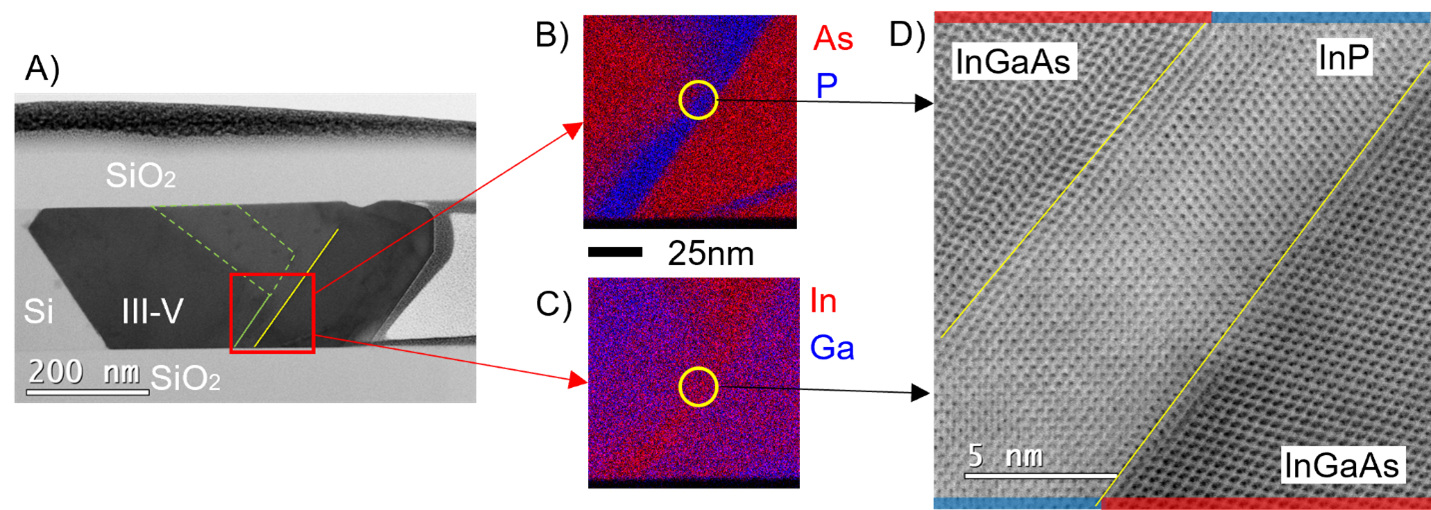
\includegraphics{3_Growth/ICMOVPEXXFig3.png
%        }
%    }
%    \caption{STEM image and EDS maps of a lamella cut from the growth experiments carried out with the recipe shown in Figure 1. A) Overview of bright-field STEM image of the nanowire. The growth front for the InGaAs layer is highlighted in green, with the dashed line indicating one of the (tilted) {110} planes and the solid line indicating the {111} plane. The {111} growth front for the InP layer is highlighted in yellow. B) EDS map of the region highlighted by the red square in (A), red As, blue P concentration. C) Corresponding EDS map with red In, blue Ga concentration. D) High-resolution image of the heterostructure region. }
%    \label{fig:ICMOVPEXXFig3}
%\end{figure}

%The first sample was grown using the precursor sequence shown in Figure 1.A PRECURSOR SWITCHING REFERENCE which serves as a reference structure for the growth optimisation study. Figure~\ref{fig:ICMOVPEXXFig3}.A shows the bright field (B.F.-)STEM image of the cross-section of a nanowire grown from left to right. %The small size of the P atoms compared to the As atoms make the InP region appear lighter than the InGaAs region because of the channelling contrast. %The growth rates of the low-index facets depend on the specific growth conditions and vary with T and V/III ratio \cite{Elsner1992}. 
%The silicon seed on the left side has two {111} facets on which the III-V material nucleated and grew into an InGaAs segment, with InP in between. 

%The InGaAs terminates in a multi-faceted front, with two inclined {110} facets at the top and one {111} facet at the bottom. This is a common growth front morphology for InGaAs nanowires along the in-plane <110> direction and originates from the availability of five energetically equivalent {110} facets and two polar {111}A or {111}B facets. 

%In contrast, the InP base layer grows much faster using high V/III ratios in the <110> direction compared to the <111> direction, leading to a large, single  \hkl{111}\(_B\) facet as the evolving growth front, as indicated by the yellow line in figure 3.A. 
%Therefore, an InP segment is preferred as a starting point for the growth of well-defined heterostructures in this geometry. 

%The compositional transition profiles of the heterostructures resulting from the reference recipe are evaluated using high-resolution EDS maps, shown in Figure~\ref{fig:ICMOVPEXXFig3}.B,C. Comparing the group V map (Figure~\ref{fig:ICMOVPEXXFig3}.B) with the group III map (Figure~\ref{fig:ICMOVPEXXFig3}.C), reveals that the group V (As, P) are confined in the respective layers with well-defined interfaces while group III elements (In, Ga) show intermixing. This intermixing is particularly visible in the bottom right corner of the EDS maps, where the thin (75 s long pulse) phosphide layer does not have a corresponding In-rich (Ga-free) signal. 

%This indicates that diffusion effects in the template channels strongly affect the group-III precursor distribution, causing extensive alloying when the growth step time is similar to the timescale of the diffusive processes. An atomic resolution image of the InP layer is indicated in Figure~\ref{fig:ICMOVPEXXFig3}.B, C is presented in Figure~\ref{fig:ICMOVPEXXFig3}.D, with the yellow lines highlighting the heterointerfaces, and the red and blue lines identify the InGaAs and InP segments, respectively. 



%\begin{figure}
%    \centering
%    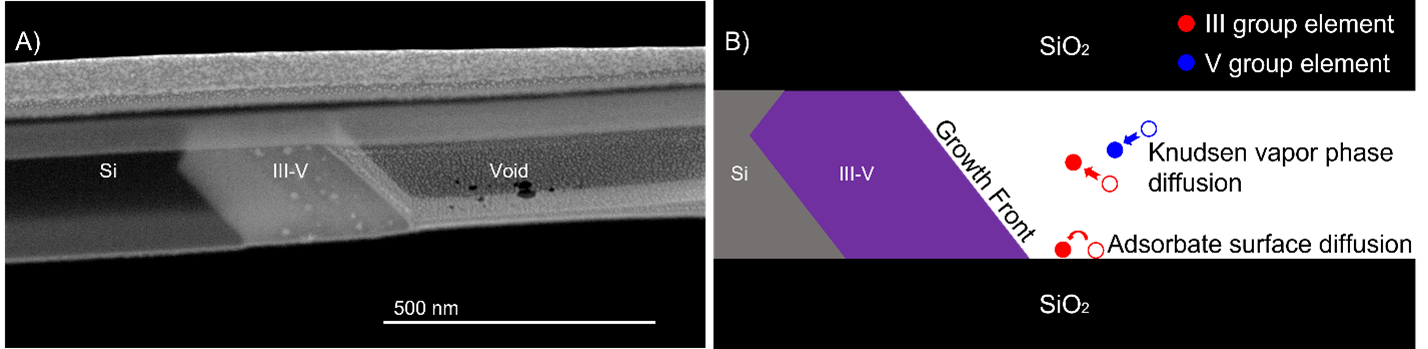
\includegraphics[width = \textwidth]{3_Growth/ICMOVPEXXFig2.png}
%    \caption{A) SEM image of a TASE-grown nanowire taken during FIB thinning. The sample is tilted 52 degrees with respect to the <001> vector defining the wafer plane. The dots are visible in the area marked as void are due to platinum deposition employed during FIB preparation. B) Schematic drawing of the various diffusion mechanisms available to III and V precursors, coloured in red and blue, respectively.}
%    \label{fig:ICMOVPEXXFig2}
%\end{figure}

%When optimising the growth recipe in selective area growth and TASE, it is important to consider the template geometry's effect on the precursors' diffusion towards the growth front. A scanning electron microscopy (SEM) image taken during focused ion beam (FIB) thinning of a nanowire cross-section (Figure 2.A) serves to illustrate a typical geometry with the Si seed on the left and the TASE-grown III-V wire in the centre. The precursor diffusion routes are shown schematically in Figure~\ref{fig:ICMOVPEXXFig2}.B, indicating that III-group elements (red) can diffuse both in the vapour phase, through Knudsen diffusion, and inside the confined space of the template on the SiO2 surface as adsorbates. This means that one slow extra diffusional route is available for them compared to the fast vapour phase diffusion mechanism that is predominantly available to the V-group precursors and atoms \cite{Borg2015}, represented in blue in Figure~\ref{fig:ICMOVPEXXFig2}.B. These different transport channels can lead to loss of interface sharpness and composition control of III-V heterostructures and need to be accounted for. 



%\begin{figure}
%    \centering
%    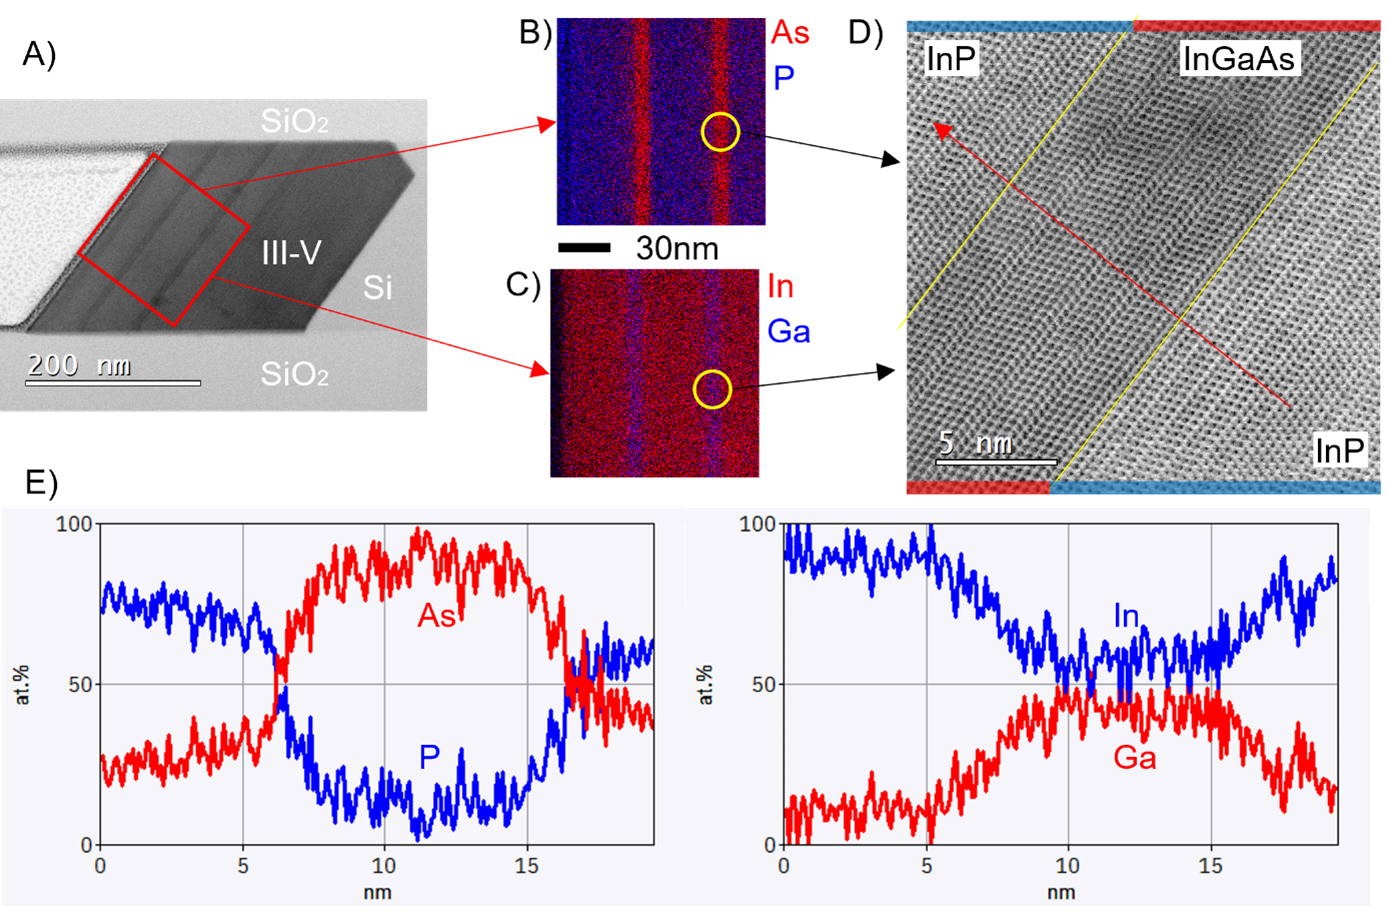
\includegraphics[width=\textwidth]{3_Growth/ICMOVPEXXFig4.png}
%    \caption{STEM image, EDS maps, and line scan of the growth experiments carried out with the recipe in Figure 2. A) Overview BF-STEM image of the nanowire. B) Color-coded EDS map of the region highlighted by the red square in (A), red As, blue P concentration, respectively. C) Color-coded EDS map of the region highlighted by the red square in (A), red In, and blue Ga concentration, respectively. D) BF-STEM detail of the 10-nm-thick InGaAs heterolayer marked by the yellow circle in (B,C). E) EDS line-scan spectra recorded across the InGaAs well as highlighted in (D) by the red arrow showing scan direction.}
%    \label{fig:ICMOVPEXXFig4}
%\end{figure}

%Based on the previous results, an optimised recipe sequence, including purge steps, was implemented, as indicated in Figure 1.B. The experimental result is shown in a BF-STEM cross-section image in Figure~\ref{fig:ICMOVPEXXFig4}.A. The sample is recorded with the Si seed on the right-hand side of the image, from which a first InGaAs nucleation layer is grown, followed by a first InP layer, similarly to the procedure followed in the growth of the sample in Figure~\ref{fig:ICMOVPEXXFig3}.

%The stabilisation of the growth front into a single {111} facet during InP growth is accomplished again. However, the first differences can be readily observed in the sample. 
%The introduction of hold steps in the growth recipe maintains this {111} growth front throughout the \acl{qw} region, creating well-defined, flat, and reproducible hetero layers. 
%The single-facet growth front avoids issues related to different incorporation rates and thickness variations with a multi-faceted growth front \cite{Borg2019}. 
%InGaAs and InP deposition time change to 30 s and 180 s create 9-nm-wide InGaAs \acl{qw}s evenly spaced between 41-nm-wide InP base layers. The \hkl<111>\(_B\) growth rates extracted are 13.9 nm/min for InP and 18.5 nm/min for InGaAs, respectively. 
%The chemical composition of the heterointerface was investigated with EDS. The V-group and III-group element concentration maps are shown in Figure~\ref{fig:ICMOVPEXXFig4}.B and C, respectively, indicating the suppression of intermixing between the two III-V materials. A high-resolution ADF-STEM image of the first InGaAs well is presented in Figure 4.D and shows that the only defects present are twin planes consistent with growth along the <111>B direction \cite{Borg2019}. The difference in channelling contrast in the InP region at the top left and bottom right of Figure 4.D, together with the red background in InGaAs layers in Figure~\ref{fig:ICMOVPEXXFig4}.B are indications of a small amount of As in the InP region. 

%This is further supported by the EDS line scan across the InGaAs \acl{qw} shown in Figure~\ref{fig:ICMOVPEXXFig4}.E. 

%Here, the atomic percentage of each group-V element is calculated from the characteristic K lines in the EDS spectra at 10.5 keV for As and at 2 keV for P. 

%The higher As level observed in the InP layer after the second interface indicates As carry-over contamination, which is not found after the first heterointerface. 

%The qualitative composition of the InxGa1-xAs layer was obtained using the relative intensities of the L lines of In and Ga, at 3.3 keV and 1.1 keV, respectively, as the In K line is not in the detector spectral range (Figure~\ref{fig:ICMOVPEXXFig4}.E, right side). Given the high noise fluctuations of the concentration profiles, a value of x = 0.55 of the InxGa1-xAs is extracted. This molar fraction, as discussed, represents an indicative data point, not only because of the noise but also because the calculation uses the standard EDS cross sections available with the Gatan Microscopy suite, and there has not been a further in-house calibration.




\chapter{Crystalline properties of TASE-grown nanowires}
\label{chap:properties}

The critical growth mechanisms and single-facet \hkl{111}\(_B\) growth front stabilisation method were explored and developed in Chapter~\ref{chap:growth}. However, the lack of in-plane \hkl{1 1 1} directions in the \hkl(0 0 1) \acf{soi} wafer on which growth was carried out complicates the analysis of the growth results. The two possible \hkl{1 1 1} facets are tilted and, therefore, yield calculations and contacting of devices become more complex, as the process through which one of the facets is selected for stabilisation is dependent on the shape and orientation of the nucleating crystal on the \acs{si} seed.

CHAPTER OVERVIEW

\section{\texorpdfstring{Fabrication on \acs{si}\hkl(1 1 0) \acs{soi}}{Fabrication on Si(110) SOI}}

The fabrication of templates for nanowires and microstructures on the new \hkl(1 1 0) substrate followed the same underlying methodology (see Appendix~\ref{chap:tase}) implemented on the same tools (see Appendix~\ref{chap:tools}) that was used for the samples in Chapter~\ref{chap:growth}. A series of lithography steps, including both \acf{ebl} and uv lithography; deposition steps, including \acf{ald} and \acf{pecvd}; and etching steps, including \acf{rie}, \acf{icp} etching and \acf{tmah} and \acf{hf} etching were employed to define the structures (seed and growth region) enclose them in the template \acs{sio2}, open the template, and finally etch back the sacrificial \acs{si} to expose the seed surface.

\subsection{Template design considerations}


\begin{figure}
    \centering
    \subcaptionbox{
    \hkl(1 1 0) in-plane crystalline directions.
    \label{subfig:110wafer_directions}
    }{
        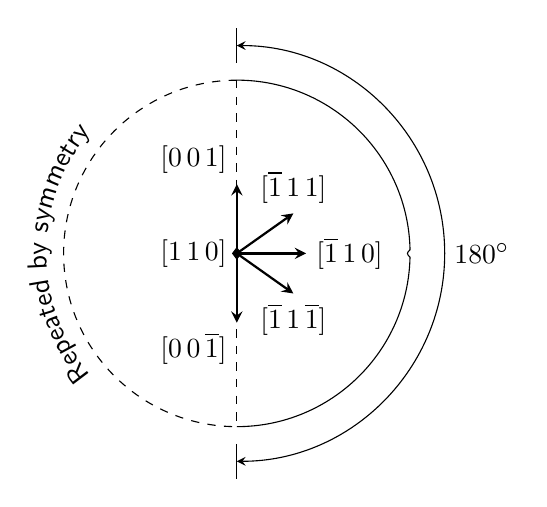
\begin{tikzpicture}
            \begin{scope}[scale=0.22]
                \draw (90:11cm) -- (90:13cm);
                \draw[stealth-stealth] (90:12cm) arc [start angle = 90, end angle = -90, radius = 12cm] node[midway, anchor = west]{\qty{180}{\degree}};
                \draw (-90:11cm) -- (-90:13cm);
                \draw (-90:10cm) arc [start angle=270, end angle=358.8, radius=10cm] -- (9.8935cm,-1.065mm) arc [start angle=-135, end angle=-225, radius=1.5mm] -- (9.9987cm,2.13mm) arc [start angle=1.20, end angle=90, radius=10cm];
                \draw[dashed] (90:10cm) arc [start angle=90, end angle=270, radius=10cm];
                \path[decorate,decoration={text along path, text={Repeated by symmetry},text align=center}] (315:11) arc [start angle=315,end angle=45,radius=11];
                \draw[dashed] (90:10cm) -- (0, 0) -- (-90:10cm);
                \draw[-stealth, thick] (0, 0) -- ++ (90:4cm) node[anchor=south east] {\hkl[0 0 1]};
                \draw[-stealth, thick] (0, 0) -- ++ (35.3:4cm) node[anchor=south] {\hkl[-1 1 1]};
                \draw[-stealth, thick] (0, 0) node[anchor=east] {\hkl[1 1 0]} -- ++ (0:4cm) node[anchor=west] {\hkl[-1 1 0]};
                \draw[-stealth, thick] (0, 0) -- ++ (270:4cm) node[anchor=north east] {\hkl[0 0 -1]};
                \draw[-stealth, thick] (0, 0) -- ++ (-35.3:4cm) node[anchor=north] {\hkl[-1 1 -1]};
                \node[mark size=2pt] at (0, 0) {\pgfuseplotmark{diamond*}};
            \end{scope}
        \end{tikzpicture}
    }
    \subcaptionbox{
    \acs{si} seed area before growth.
    \label{subfig:110_etchback}
    }{
        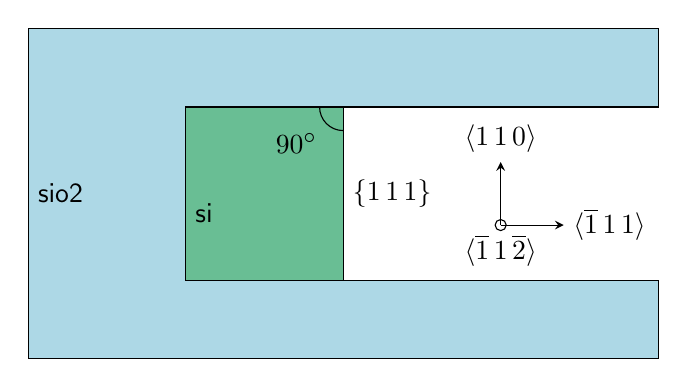
\begin{tikzpicture}
            \filldraw[fill=Si_green] (2cm, 0cm) --  node[midway, anchor= north west] {\acs{si}} (2cm, 22mm) -- (4cm, 22mm) -- (4cm, 0cm) node[midway, anchor=west]{{\hkl{1 1 1}}} -- cycle;
            \filldraw[fill=SiO2_blue] (0cm, -10mm) -- (8cm, -10mm) -- (8cm, 0cm) -- (2cm, 0mm)-- (2cm, 22mm) -- (8cm, 22mm) -- (8cm, 32mm) -- (0cm, 32mm) --  node[midway, anchor=west] {\acs{sio2}} cycle; 
            \draw (3.7cm, 22mm) arc [start angle = 180, end angle = 270, radius = 3mm] node[midway, anchor = north east]{\qty{90}{\degree}};
            \draw[-stealth] (6cm, 7mm) node[anchor=north] {\hkl<-1 1 -2>} -- ++ (90:0.8cm) node[anchor=south] {\hkl<1 1 0>};
            \draw[-stealth] (6cm, 7mm) -- ++ (0:0.8cm) node[anchor=west] {\hkl<-1 1 1>};
            \node[mark size=2pt] at (6, 7mm) {\pgfuseplotmark{o}};
        \end{tikzpicture}
    }
    \caption{Crystalline orientations in the \hkl[1 1 0] \acs{soi} wafer. \subref{subfig:110wafer_directions} shows a schematic of the crystalline directions in the plane of the \acs{si} device layer, highlighting its two-fold symmetry. \subref{subfig:110_etchback} highlights the high-symmetry directions in the \hkl{1 1 2} plane containing the chosen \hkl<1 1 1> growth direction and the \hkl[1 1 0] vector defining the wafer orientation. It highlights the vertical \hkl{1 1 1} seed facet.}
    \label{fig:110_wafer_properties}
\end{figure}

An initial evaluation of the crystalline symmetry in the wafer plane is necessary to plan the orientation of the \acf{tase} templates on the wafer surface. Figure~\ref{subfig:110wafer_directions} shows the various in-plane crystalline directions in the top device layer of the \hkl(1 1 0) \acs{soi} wafer employed in the fabrication of all future samples. Unlike its \hkl(001) predecessor, which had a four-fold axis perpendicular to the wafer plane, this \hkl(1 1 0) wafer has a two-fold axis dictating the in-plane symmetry. Therefore, the wafer's notch becomes key to orienting the \acs{tase} structures with the desired crystalline directions.
\par
Figure~\ref{subfig:110_etchback} shows a schematic cross-section of the \acs{tase} structure before growth with colour-coded materials. The \acs{si} seed presents a \hkl{1 1 1} facet forming a \qty{90}{\degree} angle with all the template walls because of the \acs{tmah} etchant used to remove the sacrificial \acl{si}; unlike the \hkl<0 0 1> wafer samples which formed \qty{90}{\degree} angles with the sidewalls (Figure~\ref{subfig:enterprise_etchback}).

\begin{sidewaysfigure}
    \centering
    \subcaptionbox{
    Double comb structure evolution from the comb structure in Figure~\ref{subfig:enterprise_design}.
    \label{subfig:110_design1}
    }{
        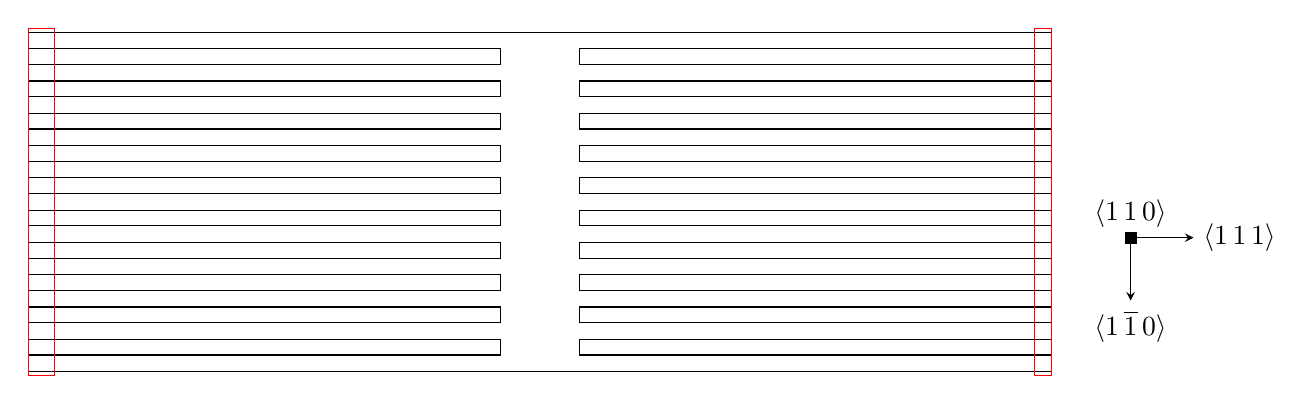
\begin{tikzpicture}
            \begin{scope}[]
                \draw (0, 0) -- ++ (13, 0) -- ++ (0, 0.21) -- ++ (-6, 0) -- ++ (0, 0.2) -- ++ (6, 0) -- ++ (0, 0.21) -- ++ (-6, 0) -- ++ (0, 0.2) -- ++ (6, 0) -- ++ (0, 0.21) -- ++ (-6, 0) -- ++ (0, 0.2) -- ++ (6, 0) -- ++ (0, 0.21) -- ++ (-6, 0) -- ++ (0, 0.2) -- ++ (6, 0) -- ++ (0, 0.21) -- ++ (-6, 0) -- ++ (0, 0.2) -- ++ (6, 0) -- ++ (0, 0.21) -- ++ (-6, 0) -- ++ (0, 0.2) -- ++ (6, 0) -- ++ (0, 0.21) -- ++ (-6, 0) -- ++ (0, 0.2) -- ++ (6, 0) -- ++ (0, 0.21) -- ++ (-6, 0) -- ++ (0, 0.2) -- ++ (6, 0) -- ++ (0, 0.21) -- ++ (-6, 0) -- ++ (0, 0.2) -- ++ (6, 0) -- ++ (0, 0.21) -- ++ (-6, 0) -- ++ (0, 0.2) -- ++ (6, 0) -- ++ (0, 0.21) -- ++ (-13, 0) -- ++ (0, -0.21) -- ++ (6, 0) -- ++ (0, -0.2) -- ++ (-6, 0) -- ++ (0, -0.21) -- ++ (6, 0) -- ++ (0, -0.2) -- ++ (-6, 0) -- ++ (0, -0.21) -- ++ (6, 0) -- ++ (0, -0.2) -- ++ (-6, 0) -- ++ (0, -0.21) -- ++ (6, 0) -- ++ (0, -0.2) -- ++ (-6, 0) -- ++ (0, -0.21) -- ++ (6, 0) -- ++ (0, -0.2) -- ++ (-6, 0) -- ++ (0, -0.21) -- ++ (6, 0) -- ++ (0, -0.2) -- ++ (-6, 0) -- ++ (0, -0.21) -- ++ (6, 0) -- ++ (0, -0.2) -- ++ (-6, 0) -- ++ (0, -0.21) -- ++ (6, 0) -- ++ (0, -0.2) -- ++ (-6, 0) -- ++ (0, -0.21) -- ++ (6, 0) -- ++ (0, -0.2) -- ++ (-6, 0) -- ++ (0, -0.21) -- ++ (6, 0) -- ++ (0, -0.2) -- ++ (-6, 0) -- ++ (0, -0.21);
                \draw[red] (0, -0.05) rectangle (0.333, 4.36);
                \draw[red] (12.777, -0.05) rectangle (13, 4.36);
            \end{scope}
            \begin{scope}[shift={(14cm, 1.7cm)}]
                \draw[-stealth] (0cm, 0cm) -- ++ (-90:0.8cm) node[anchor=north] {\hkl<1 -1 0>};
                \draw[-stealth] (0cm, 0cm)  node[anchor=south] {\hkl<1 1 0>} -- ++ (0:0.8cm) node[anchor=west] {\hkl<1 1 1>};
                \node[mark size=2pt] at (0, 0) {\pgfuseplotmark{square*}};
            \end{scope}
        \end{tikzpicture}
    }
    \subcaptionbox{
    Array structure evolved from the double comb structure of \subref{subfig:110_design1} and merge wire structure on the bottom right.
    \label{subfig:110_design2}
    }{
        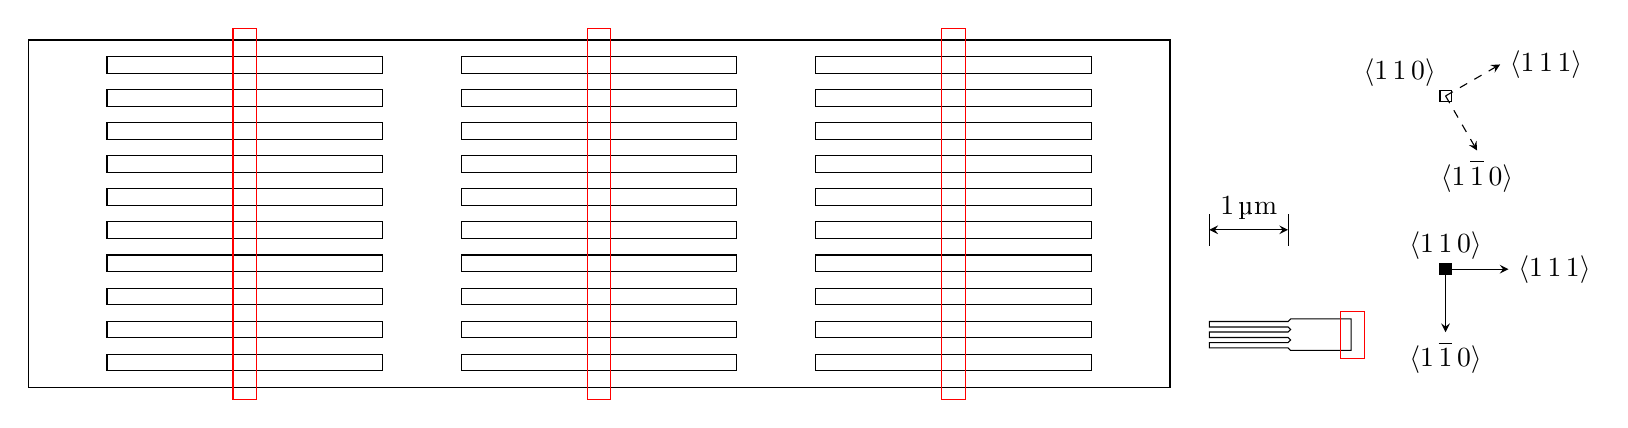
\begin{tikzpicture}
            \begin{scope}
                \draw (0, 0) rectangle (14.5, 4.41);
                \foreach \x in {1, 5.5, 10}
                    \foreach \y in {1, 3, 5, 7, 9, 11, 13, 15, 17, 19}
                        \draw (\x, \y*0.21) rectangle (\x+3.5, 0.21+\y*0.21);
                \foreach \x in {2.6, 7.1, 11.6}
                    \draw [red] (\x, -0.15) rectangle (\x+0.3, 4.56);
            \end{scope}
            \begin{scope}[shift={(15cm, 0.5cm)}]
                \draw (0,0) -- ++ (1, 0) -- ++ (-45:0.045255) -- ++ (0.768, 0) -- ++ (0, 0.4) -- ++ (-0.768, 0) -- ++ (-135:0.045255) -- ++ (-1, 0) -- ++ (0, -0.07) -- ++ (1, 0) -- ++ (-45:0.045255) -- ++ (-135:0.045255) -- ++ (-1, 0) -- ++ (0, -0.07) -- ++ (1, 0) -- ++ (-45:0.045255) -- ++ (-135:0.045255) -- ++ (-1, 0) -- cycle;
                \draw [red] (1.668, -0.132) rectangle (1.968, 0.468);
                \draw[stealth-stealth] (0, 1.5) -- (1, 1.5) node [midway, anchor = south] {\qty{1}{\micro\metre}};
                \draw (0, 1.3) -- (0, 1.7);
                \draw (1, 1.3) -- (1, 1.7);
            \end{scope}
            \begin{scope}[shift={(18cm, 1.5cm)}]
                \draw[-stealth] (0cm, 0cm) -- ++ (-90:0.8cm) node[anchor=north] {\hkl<1 -1 0>};
                \draw[-stealth] (0cm, 0cm)  node[anchor=south] {\hkl<1 1 0>} -- ++ (0:0.8cm) node[anchor=west] {\hkl<1 1 1>};
                \node[mark size=2pt] at (0, 0) {\pgfuseplotmark{square*}};
            \end{scope}
            \begin{scope}[shift={(18cm, 3.7cm)}, rotate=30]
                \draw[-stealth, dashed] (0cm, 0cm) -- ++ (-90:0.8cm) node[anchor=north] {\hkl<1 -1 0>};
                \draw[-stealth, dashed] (0cm, 0cm)  node[anchor=south east] {\hkl<1 1 0>} -- ++ (0:0.8cm) node[anchor=west] {\hkl<1 1 1>};
                \node[mark size=2pt] at (0, 0) {\pgfuseplotmark{square}};
            \end{scope}
        \end{tikzpicture}
    }
    \caption{Microstructure designs for \acs{tase} growth. The structures transferred to the \acs{si} device layer are represented in black and the template opening regions in red. \subref{subfig:110_design1} shows the double comb structures grown on the first \hkl[1 1 0] samples. These were always oriented to have the template axis coincide with the in-plane \hkl<1 1 1> directions. \subref{subfig:110_design2} shows the nanowire array structures used in later experiments on the \hkl[1 1 0] \acs{soi}s and the "merge wire" structures. These types of structures were grown both aligned with the in-plane \hkl[1 1 1] direction, as highlighted by the solid-line arrows, and \qty{30}{\degree} misaligned, as shown by the dashed arrows \cite{Brugnolotto2023_2}.}
    \label{fig:110_Template_Design}
\end{sidewaysfigure}

Figure~\ref{fig:110_Template_Design} shows the evolution of the \acs{tase} structures from those in Figure~\ref{fig:001_Templat5e_Design}. The comb structure of Figure~\ref{subfig:enterprise_design} is perfect for \acf{sem_m} analysis of multiple wires in a single image and the \acf{stem_m} survey of cross-section cuts perpendicular to the growth direction. However, cross-sections parallel to the growth direction only allow for the analysis of a single wire.
\par
As the analysis of heterointerfaces stacked along the growth vector is the primary goal of this work, maximising the number of wires observable from seed to final interface in a single \acf{fib} cut is a key objective of the design phase. Taking inspiration from the "T-shaped" structure in Figure~\ref{subfig:enterprise_design} the first evolution of the comb array is shown in Figure~\ref{subfig:110_design1}. A central rectangular \acs{si} backbone anchors two rows of nanowires that extend from either side, with the templates being open at the very edges of the structure (in red in Figure~\ref{subfig:110_design1}. The length of the nanowire growth area extends up to \qty{7}{\micro\metre} for this design. These long channels (in relation to their \qty{70}{\nano\metre} height) were designed to study the effect of growth in "deep" templates on resulting composition and growth rates. Unfortunately, in practice, the resulting structure could only be used with short etch-back segments. This was due to the thickness of the side walls in the final samples, which was insufficient to ensure structural integrity during \acs{tmah} etch-back, despite the selectivity of this etchant.
\par
The difficulties encountered with the design in Figure~\ref{subfig:110_design1} together with the possibility of having more \acs{stem_m}-observable nanowires per \acs{fib} cut led to the design of the array structure in Figure~\ref{subfig:110_design2}. This allows for the \acs{stem_m} analysis of \num{6} short nanowires up to \qty{2}{\micro\metre}-long while keeping the overall length of the structure at \qty{14.5}{\micro\metre}, and therefore comparable to that of the double-comb design (\qty{13}{\micro\metre}). There are \num{4} equidistant rectangular backbone anchors, with two marking the beginning and end of the structure. The templates are open between the anchors in three areas of the structures (in red in Figure~\ref{subfig:110_design2}). Thus, once complete, one such array contains \num{66} growth sites.

Wire widths of \qty{70}{\nano\metre}, \qty{140}{\nano\metre}, \qty{210}{\nano\metre}, and \qty{280}{\nano\metre} were fabricated, the Figures~\ref{subfig:110_design1} and \ref{subfig:110_design2} show the \qty{210}{\nano\metre} designs.

To the bottom right of the array in Figure~\ref{subfig:110_design2} there is a "merge wire" structure. In this structure, three nucleation wires with a design width of \qty{70}{\nano\metre} all terminate in a single channel \qty{400}{\nano\metre} wide. This structure was designed to study the merging regions between the three growing crystals to observe the defects that could form from the merging of two growing crystals. In the past, it was employed to demonstrate the introduction of dislocations in \acs{tase} microstructures \cite{Mauthe2021} and published research highlighted the formation of defects at those sites due to minuscule misalignments of the crystals \cite{Jacobsson2015, Rossi2023}.

Both structures in Figure~\ref{subfig:110_design2} were grown aligned to the in-plane \hkl<1 1 1> direction but also \qty{30}{\degree} misaligned. In practice, this was done by aligning one set of structures to an in-plane \hkl<1 1 1> direction and rotating each subsequent set by \qty{90}{\degree}. Selecting this specific \qty{30}{\degree} misalignment as a basis for analysis therefore has two advantages:
\begin{enumerate}
    \item the resulting seed surfaces and projected growth fronts are at a significant angle with the template sidewalls
    \item there is no need to keep track of the direction of the notch past the dicing stage which resulted in the initial \qtyproduct{6 x 6}{cm} die.
\end{enumerate}

\subsection{\texorpdfstring{\acs{fib} lamella fabrication}{FIB lamella fabrication}}

\begin{figure}
    \centering
    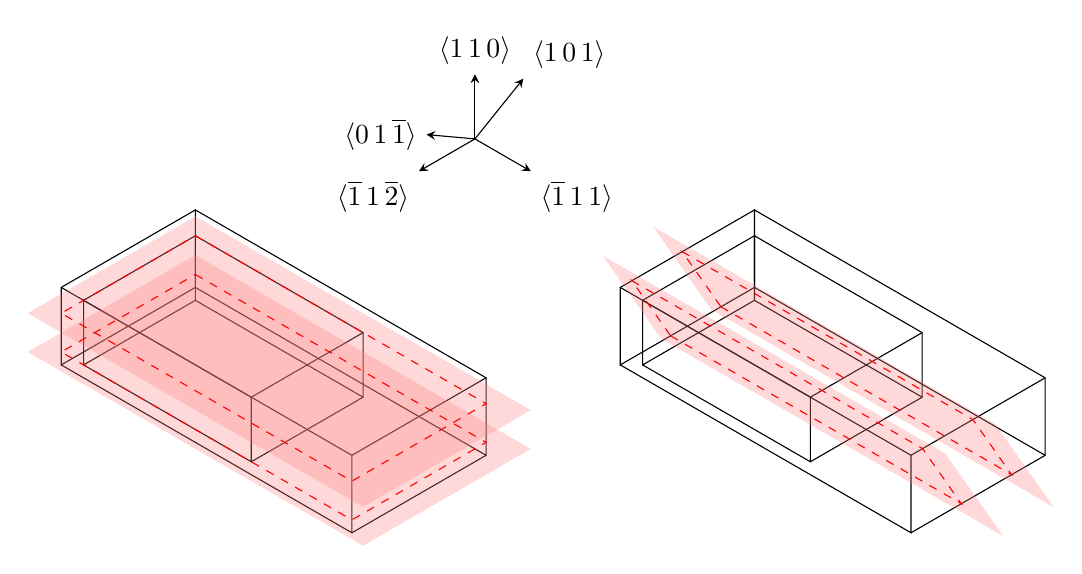
\begin{tikzpicture}[isometric]
        \draw (0, 0, 0) -- (0, 0, 2) -- (0, 1, 2) -- (0, 1, 0) -- cycle;
        \draw (0, 0, 0) -- (3, 0, 0) -- (3, 1, 0) -- (0, 1, 0);
        \draw (0, 0, 2) -- (3, 0, 2) -- (3, 1, 2) -- (0, 1, 2);
        \draw (3, 0, 0) -- (3, 0, 2);
        \draw (3, 1, 0) -- (3, 1, 2);
            
        \draw (-0.2, 0, -0.2) -- (-0.2, 0, 2.2) -- (-0.2, 1.2, 2.2) -- (-0.2, 1.2, -0.2) -- cycle;
        \draw (-0.2, 0, -0.2) -- (5, 0, -0.2) -- (5, 1.2, -0.2) -- (-0.2, 1.2, -0.2);
        \draw (-0.2, 0, 2.2) -- (5, 0, 2.2) -- (5, 1.2, 2.2) -- (-0.2, 1.2, 2.2);
        \draw (5, 0, -0.2) -- (5, 0, 2.2);
        \draw (5, 1.2, -0.2) -- (5, 1.2, 2.2);
            
        \path [fill=red!50!, fill opacity=0.3] (-0.5, 0.2, -0.5) -- (-0.5, 0.2, 2.5) -- (5.5, 0.2, 2.5) -- (5.5, 0.2, -0.5) -- cycle;
        \path [fill=red!50!, fill opacity=0.3] (-0.5, 0.8, -0.5) -- (-0.5, 0.8, 2.5) -- (5.5, 0.8, 2.5) -- (5.5, 0.8, -0.5) -- cycle;
            
        \draw [red, dashed] (-0.2, 0.2, -0.2) -- (5, 0.2, -0.2) -- (5, 0.2, 2.2) -- (-0.2, 0.2, 2.2) -- cycle;
        \draw [red, dashed] (-0.2, 0.8, -0.2) -- (5, 0.8, -0.2) -- (5, 0.8, 2.2) -- (-0.2, 0.8, 2.2) -- cycle;

        \begin{scope}[shift={(6, 6, 1)}]
            \draw [-stealth] (0, 0, 0) -- ++ (1, 0, 0) node[anchor = north west]{\hkl<-1 1 1>};
            \draw [-stealth] (0, 0, 0) -- ++ (0, 1, 0) node[anchor = south]{\hkl<1 1 0>};
            \draw [-stealth] (0, 0, 0) -- ++ (0, 0.5, 0.866) node[anchor = east]{\hkl<0 1 -1>};
            \draw [-stealth] (0, 0, 0) -- ++ (0, 0.5, -0.866) node[anchor = south west]{\hkl<1 0 1>};
            \draw [-stealth] (0, 0, 0) -- ++ (0, 0, 1) node[anchor = north east]{\hkl<-1 1 -2>};
        \end{scope}

        \begin{scope}[shift={(10, 5, 0)}]
            \draw (0, 0, 0) -- (0, 0, 2) -- (0, 1, 2) -- (0, 1, 0) -- cycle;
            \draw (0, 0, 0) -- (3, 0, 0) -- (3, 1, 0) -- (0, 1, 0);
            \draw (0, 0, 2) -- (3, 0, 2) -- (3, 1, 2) -- (0, 1, 2);
            \draw (3, 0, 0) -- (3, 0, 2);
            \draw (3, 1, 0) -- (3, 1, 2);
            
            \draw (-0.2, 0, -0.2) -- (-0.2, 0, 2.2) -- (-0.2, 1.2, 2.2) -- (-0.2, 1.2, -0.2) -- cycle;
            \draw (-0.2, 0, -0.2) -- (5, 0, -0.2) -- (5, 1.2, -0.2) -- (-0.2, 1.2, -0.2);
            \draw (-0.2, 0, 2.2) -- (5, 0, 2.2) -- (5, 1.2, 2.2) -- (-0.2, 1.2, 2.2);
            \draw (5, 0, -0.2) -- (5, 0, 2.2);
            \draw (5, 1.2, -0.2) -- (5, 1.2, 2.2);

            \path [fill=red!50!, fill opacity=0.3] (-0.54641016, -0.3, 0.22679492) -- (-0.54641016, 1.5, 1.2660254) -- (5.57735027, 1.5, 1.2660254) -- (5.57735027, -0.3, 0.22679492) -- cycle;
            \path [fill=red!50!, fill opacity=0.3] (-0.54641016, -0.3, 1.12679492) -- (-0.54641016, 1.5, 2.1660254) -- (5.57735027, 1.5, 2.1660254) -- (5.57735027, -0.3, 1.12679492) -- cycle;
        
            \draw [red, dashed] (-0.2, 0, 0.4) -- (5, 0, 0.4) -- (5, 1.2, 1.09282032) -- (-0.2, 1.2, 1.09282032) -- cycle;
            \draw [red, dashed] (-0.2, 0, 1.3) -- (5, 0, 1.3) -- (5, 1.2, 1.99282032) -- (-0.2, 1.2, 1.99282032) -- cycle;
        \end{scope}
    \end{tikzpicture}
    \caption{\acs{fib} cutting strategies to expose \hkl{1 1 0} facets from a \hkl[1 1 0]-oriented substrate. The red-shaded planes show how the cut planes are selected to expose the sides of the wire in correspondence to \hkl{1 1 0} facets if the template axis coincides with a \hkl<1 1 1> direction.}
    \label{fig:110_FIB}
\end{figure}

While a new \hkl<1 1 0> wafer and \hkl<1 1 1> template orientation were used for fabrication, the preference for an exposed \hkl{1 1 0} facet for structural analysis with \acs{stem_m} remains unaltered due to this facet allowing easy recognition of a wide variety of crystalline defects \cite{Dasilva2017}. However, the first difficulty is that, as highlighted in Figure~\ref{subfig:110_etchback}, the in-plane crystalline direction perpendicular to the \hkl<1 1 1> template axis is a \hkl<1 1 2>, making the simple cross-section cut used in the previous chapter (Figure~\ref{subfig:FIB_cut_strategy}) unsuitable.

The most obvious \hkl<1 1 0> direction perpendicular to the \hkl<1 1 1> template axis is the one that defines the wafer orientation itself. As shown on the left of Figure~\ref{fig:110_FIB}, a plane-view cut would satisfy orientation requirements and allow for precise \acf{eds} composition maps and an excellent overview of the evolution of the growth front. However, such a cut is much more complex and time-consuming than a cross-sectional cut. The amount of lamella that must be thinned to sub \qty{100}{\nano\metre} thickness to ensure electron transparency increased from a few hundred nanometres to \qty{1.5}{\micro\metre}, which is challenging to do with the ion beam of the \acs{fib} and requires a high level of precision. This is particularly true when milling both sides of a target region composed of multiple material layers eroded at different rates.

A compromise can be found by cutting the sample with a \qty{30}{\degree} tilt in the stage resulting in the cutting planes drawn on the nanowire on the right in Figure~\ref{fig:110_FIB}. Referring to the direction legend in Figure~\ref{fig:110_FIB}, these expose the \hkl(1 0 1) facet, part of the family of \hkl{1 1 0} facets which all share the same symmetry in the zincblende phase (space group \num{216}) \cite{wyckoff1963crystal, osti_gaas_zb, osti_inas_zb, osti_inp_zb}. This "\qty{30}{\degree} cut" allows an analysis of the evolution of the growth front comparable to the simple cross-section cut used in the previous chapter (Figure~\ref{subfig:FIB_cut_strategy}). Still, tilt means that any material layers not perpendicular to the growth front will appear warped, and, similarly, horizontal and tilted heterointerfaces will be shaded in \acs{eds} analysis. Therefore, a limited use of the regular \qty{90}{\degree} cross section was kept at the beginning for the experiments with the \hkl<1 1 0> wafer.

\section{Application the growth recipe on the new substrate}

\begin{sidewaysfigure}
    \centering
    \subcaptionbox{
    Growth recipe for sample 4 \cite{Brugnolotto2023}. Each line represents an active flow of the corresponding precursor into the reactor. The colour of the horizontal lines represents the target material. The dashed lines are time-compressed 10 times.
    \label{subfig:recipe4}
    }{
    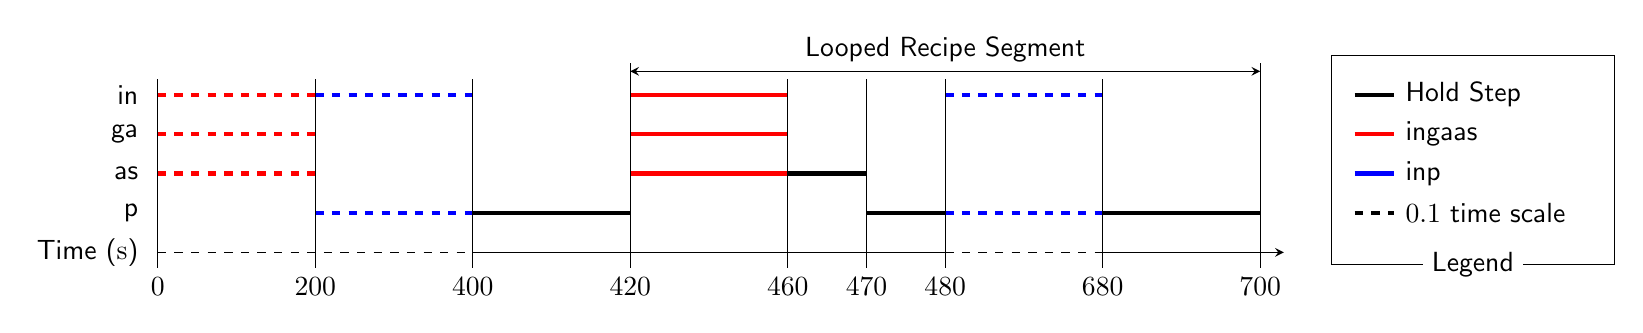
\begin{tikzpicture}
    \begin{scope}
    % lines
        \node [label={[label distance=0]180:\acs{in}}] at (0, 0) {};
        \draw [red, ultra thick, dashed] (0, 0) -- (2, 0); %/10
        \draw [blue, ultra thick, dashed] (2, 0) -- (4, 0); %10
        \draw [red, ultra thick] (6, 0) -- (8, 0);
        \draw [blue, ultra thick, dashed] (10, 0) -- (12, 0); %10
        %\draw [red, ultra thick] (7.35, 0) -- (8.1, 0);
        
        \node [label={[label distance=0]180:\acs{ga}}] at (0, -0.5) {};
        \draw [red, ultra thick, dashed] (0, -0.5) -- (2, -0.5cm); %/10
        \draw [red, ultra thick] (6, -0.5) -- (8, -0.5);
        
        \node [label={[label distance=0]180:\acs{as}}] at (0, -1) {};
        \draw [red, ultra thick, dashed] (0, -1) -- (2, -1); %/10
        \draw [red, ultra thick] (6, -1) -- (8, -1);
        \draw [ultra thick] (8, -1) -- (9, -1);
        
        \node [label={[label distance=0]180:\acs{p}}] at (0, -1.5) {};
        \draw [blue, ultra thick, dashed] (2, -1.5) -- (4, -1.5); %/10
        \draw [ultra thick] (4, -1.5) -- (6, -1.5);
        \draw [ultra thick] (9, -1.5) -- (10, -1.5);
        \draw [blue, ultra thick, dashed] (10, -1.5) -- (12, -1.5); %/10
        \draw [ultra thick] (12, -1.5) -- (14, -1.5);
        
    % labels and markers for the timescale
        \node [label={[label distance=0]180:Time (\second)}] at (0, -2) {};
        \draw [dashed] (0, -2) -- (4, -2);
        \draw [] (4, -2) -- (10, -2);
        \draw [dashed] (10, -2) -- (12, -2);
        \draw [-stealth] (12, -2) -- (14.3, -2); % +0.3
        \draw [] (0, 0.2) -- (0, -2.2) node[anchor = north] {\num{0}};
        \draw [] (2, 0.2) -- (2, -2.2) node[anchor = north] {\num{200}};
        \draw [] (4, 0.2) -- (4, -2.2) node[anchor = north] {\num{400}};
        \draw [] (6, 0.4) -- (6, -2.2) node[anchor = north] {\num{420}};
        \draw [] (8, 0.2) -- (8, -2.2) node[anchor = north] {\num{460}};
        \draw [] (9, 0.2) -- (9, -2.2) node[anchor = north] {\num{470}};
        \draw [] (10, 0.2) -- (10, -2.2) node[anchor = north] {\num{480}};
        \draw [] (12, 0.2) -- (12, -2.2) node[anchor = north] {\num{680}};
        \draw [] (14, 0.4) -- (14, -2.2) node[anchor = north] {\num{700}};
        \draw [stealth - stealth] (6, 0.3) -- (14, 0.3) node[midway, anchor=south] {Looped Recipe Segment};
    \end{scope}
    \begin{scope} [shift={(15.2cm, -0.5)}] % +0.9
        \draw [ultra thick] (0, 0.5) -- (0.5, 0.5) node[anchor = west, text=black] {Hold Step};
        \draw [red, ultra thick] (0, 0) -- (0.5, 0) node[anchor = west, text=black] {\acs{ingaas}};
        \draw [blue, ultra thick] (0, -0.5) -- (0.5, -0.5) node[anchor = west, text = black] {\acs{inp}};
        \draw [dashed, ultra thick] (0, -1) -- (0.5, -1) node[anchor = west, text = black] {\num{0.1} time scale};
        \draw (-0.3, 1) -- (3.3, 1) -- (3.3, -1.65) -- node[midway, fill = white] {Legend} (-0.3, -1.65) -- cycle;
    \end{scope}
    \end{tikzpicture}
    }
    \subcaptionbox{
    \acs{bf}-\acs{stem_m} overview images of two nanowires from sample 4. The wire on the left was cut with a regular cross-section, while the wire on the right was cut with a \qty{30}{\degree} cross-section.
    \label{subfig:s4_OV}
    }{
    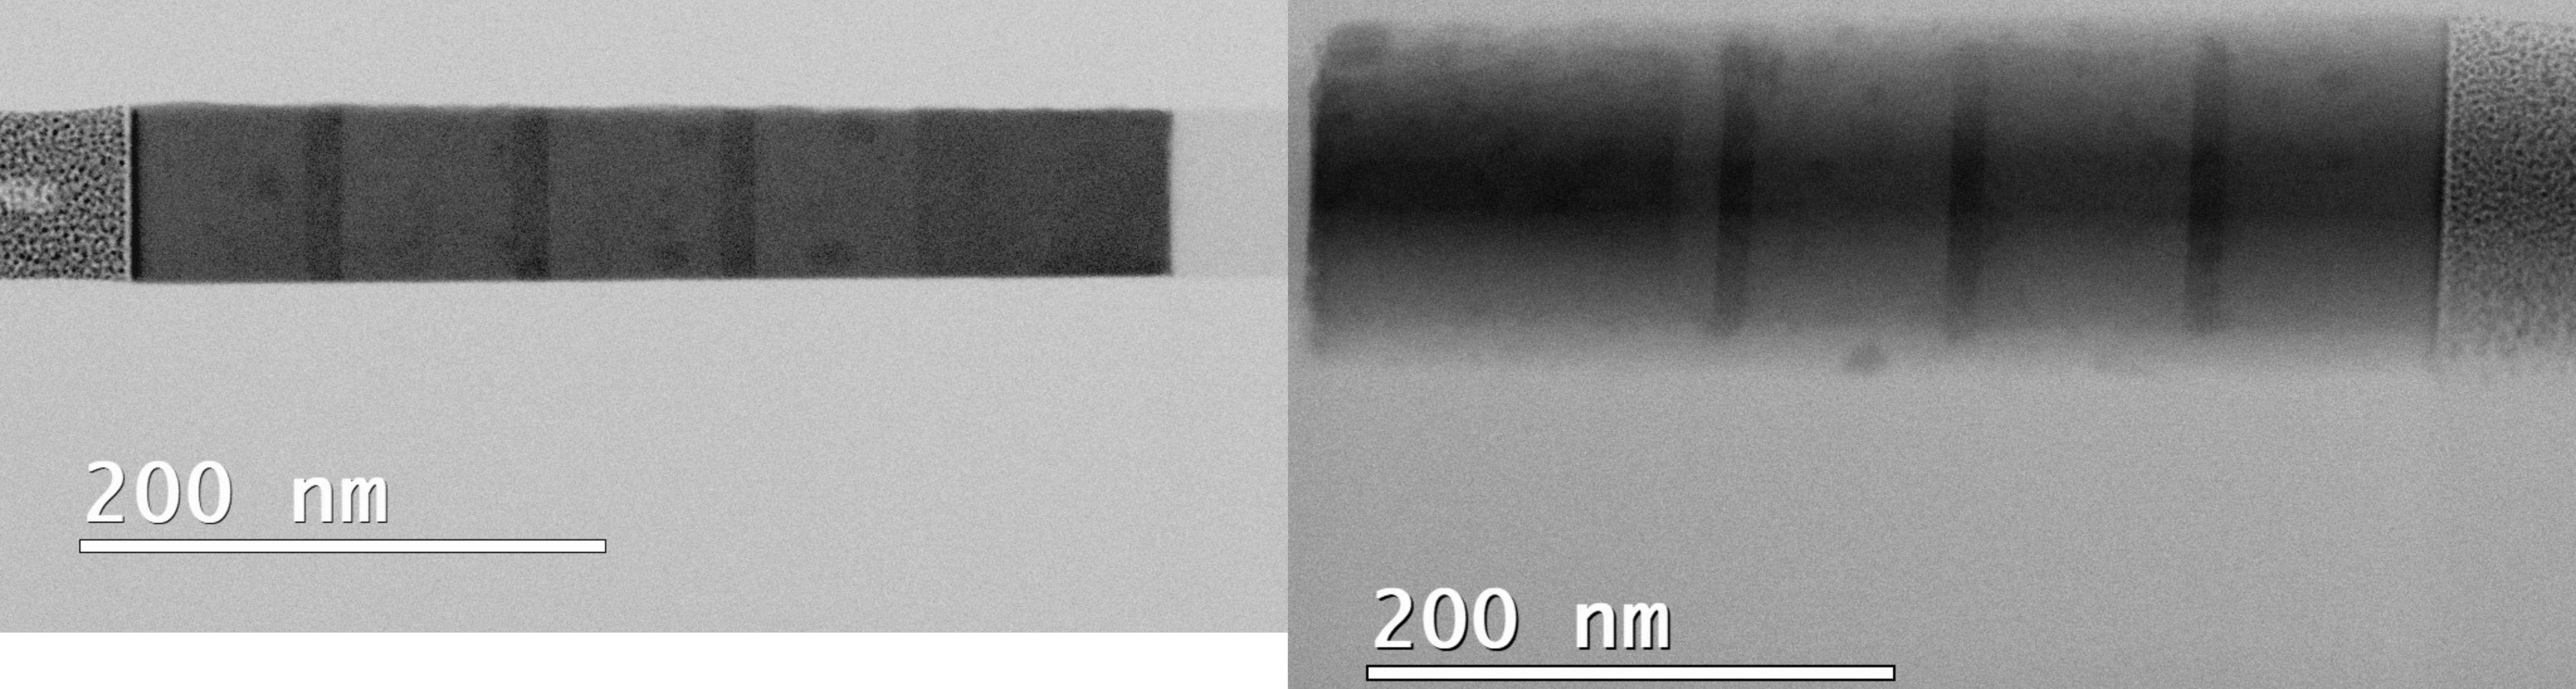
\includegraphics[width = 0.48\textwidth]{4_Crystalline_properties/Fig/s4_OV.pdf}
    }
    \subcaptionbox{
    High-resolution \acs{bf}-\acs{stem_m} images of the first \acl{qw} for both wires in \subref{subfig:s4_OV} with \acs{fft} inserts.
    \label{subfig:s4_HR}
    }{
    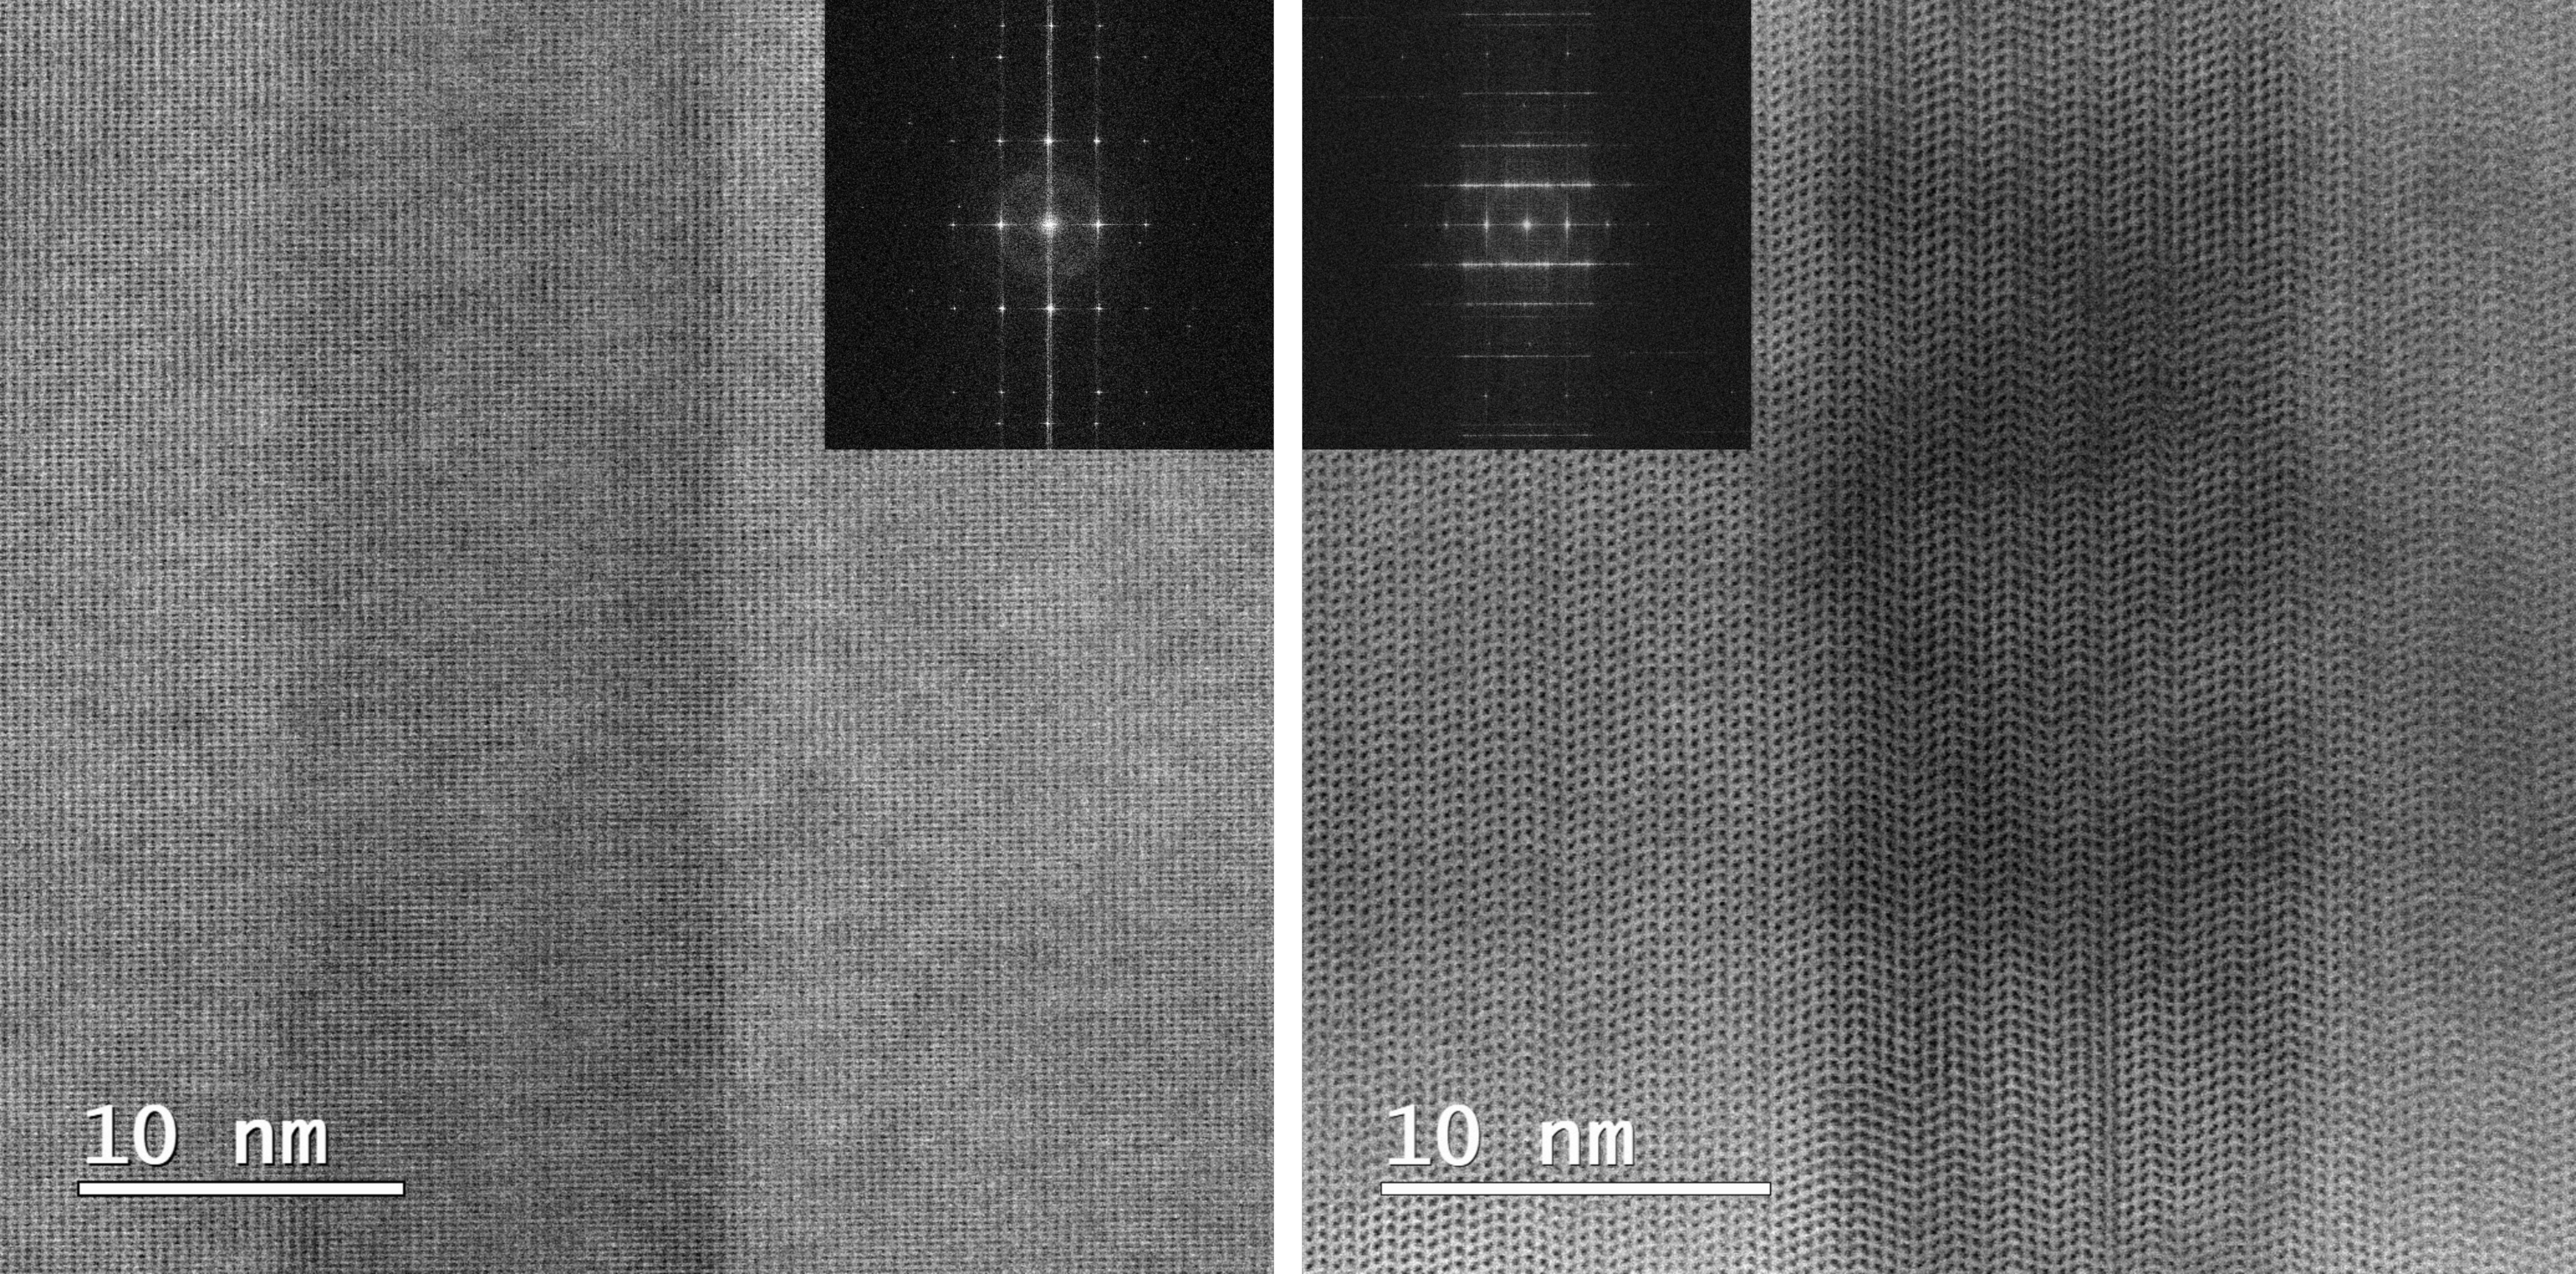
\includegraphics[width = 0.48\textwidth]{4_Crystalline_properties/Fig/s4_HR.pdf}
    }
    \caption{Growth recipe and \acs{bf}-\acs{stem_m} images of sample 4. The III-V material appears dark due to channelling contrast, with \acs{ingaas} being the darkest of the two III-V materials. \subref{subfig:recipe4} shows the growth recipe. \subref{subfig:s4_OV} shows overview images of the normal cross-section and \qty{30}{\degree} cross-section. \subref{subfig:s4_HR} shows high-resolution images of the first \acl{qw} for both wires in \subref{subfig:s4_OV} with inserts showing the calculated \acs{fft}s}
    \label{fig:s4_recipe_STEM}
\end{sidewaysfigure}

The recipe in Figure~\ref{subfig:recipe4} was kept similar to that used in sample 3 (Figure~\ref{subfig:recipe3}) for the initial experiment on the new \hkl<1 1 0> substrate. It contains a looped segment for creating \acs{ingaas} \acl{qw}s between \acs{inp} barrier layers. The main adjustments concern the deposition times. The initial growth steps, were changed from \qty{480}{\second} and \qty{180}{\second} to \qty{200}{\second} for both \acs{ingaas} and \acs{inp}, respectively. The deposition times for \acs{ingaas} \acl{qw}s were lowered from \qty{30}{\second} to \qty{20}{\second} in anticipation of the smaller area of the growth front. Simultaneously, the duration of \acs{inp} barrier steps was increased from \qty{180}{\second} to \qty{200}{\second}.

The most significant change concerned the post-\acs{ingaas} hold step. Here, \acs{as} precursor flow step time was reduced from \qty{15}{s} to \qty{10}{s} and the following \acs{p} precursor flow step time increased from \qty{5}{s} to \qty{10}{s}. This change was made to address the \acs{as} profile seen in the \acs{inp} layer of the sample 3 (Figure~\ref{subfig:s3_V_linesc}). By reducing the \acs{as} precursor flow time in the hold step it was hoped that the \acs{as} contamination in the first nanometres of the \acs{inp} layer would be reduced or, in the best case, eliminated in sample 4.

\subsection{Structural Analysis}

Figure~\ref{fig:s4_recipe_STEM} shows \acs{bf}-\acs{stem_m} images of two different wires from sample 4. The images on the left side of both Figure~\ref{subfig:s4_OV} and \ref{subfig:s4_HR} show the wire cut with a standard cross-section used in the previous chapter and schematised in Figure~\ref{subfig:FIB_cut_strategy}. In comparison, on the right side of the same figures, the images of a lamella cut with the \qty{30}{\degree} cross-section illustrated on the right of Figure~\ref{fig:110_FIB} are shown. 

Both lamellae come from the same sample, with identical device layer thickness. 
However, Figure~\ref{subfig:s4_OV} highlights how the \qty{30}{\degree} cross-section appears larger because the viewing angle is not perpendicular to the heterointerfaces that lay in the wafer plane. This distortion becomes clear when one looks at the III-V-\acs{si} interfaces at the top and bottom of the nanowires. The well-defined lines in the standard cross-section become large regions in the \qty{30}{\degree} cross-section. In these regions, the III-V nanowire and the \acs{sio2} template appear superimposed, as they are one on top of the other in the path the electron beam takes through the lamella.

An evident advantage of the \qty{30}{\degree} cut in combination with the \hkl<1 1 0> wafer is that vertical \hkl{1 1 1} heterointerfaces remain perpendicular to the viewing direction. As the recipe optimised in Chapter~\ref{chap:growth} stabilises this facet family, this new viewing angle does not affect the observer's ability to evaluate the sharpness of this type of interface from \acs{stem_m} measurements.

The comparison between the two wires at high resolution in Figure~\ref{subfig:s4_HR} also highlights the amount of structural information available when viewing a \hkl{1 1 0} plane (on the right) compared to a \hkl{1 1 2} plane (on the left). The presence of \acs{rtp}s is evident in the \qty{30}{\degree} cross-section both in the \acs{bf}-\acs{stem_m} image and in its \acf{fft} in the insert. The \acs{rtp}s have manifested as horizontal lines in the frequency domain. In contrast, both the \hkl{1 1 2} \acs{bf}-\acs{stem_m} image and its \acf{fft} do not contain any trace of this type of defect.

Both samples grew from silicon seeds that appear (in print) towards the centre of the image and grew out toward the margins. The initial \acs{ingaas} nucleation layer gives way to a lighter \acs{inp} layer in both lamellae, however, the length of this layer appears different. This could be due to a different shape of the nucleation \acs{ingaas}'s growth front. A trace of the complexity of this interface is seen at the bottom of the first well of the \qty{30}{\degree} cross-section. The bottom of this heterostructure appears bent towards the seed, suggesting that the \acs{inp} layer did not have enough time to grow to annihilate all the non-\hkl{1 1 1} facets.

\begin{table}[]
    \centering
    \caption{Growth rates for each heterolayer in the two nanowires in Figure~\ref{fig:s4_recipe_STEM}}
    \begin{tabular}{l|c c}
         & \multicolumn{2}{c}{growth rates (\nmmin)} \\
        heterolayer & \qty{0}{\degree} cross-section & \qty{30}{\degree} cross-section \\ \hline
        \acs{ingaas} nucleation & \num[separate-uncertainty=true]{29.0 (0.2)} & \num[separate-uncertainty=true]{42.4 (0.3)} \\
        \acs{inp} stabilisation & \num[separate-uncertainty=true]{18.3 (0.1)} & \num[separate-uncertainty=true]{4.7 (0.2)} \\ \hline
        \textbf{pre-wells layers} & \textbf{\num[separate-uncertainty=true]{23.7 (0.1)}} & \textbf{\num[separate-uncertainty=true]{23.6 (0.3)}} \\ \hline
        \acs{ingaas} well 1 & \num[separate-uncertainty=true]{39 (1)} & \num[separate-uncertainty=true]{35 (2)} \\
        \acs{inp} barrier 1 & \num[separate-uncertainty=true]{19.7 (0.2)} & \num[separate-uncertainty=true]{22.4 (0.1)} \\
        \acs{ingaas} well 2 & \num[separate-uncertainty=true]{41 (1)} & \num[separate-uncertainty=true]{38 (1)} \\
        \acs{inp} barrier 2 & \num[separate-uncertainty=true]{19.7 (0.2)} & \num[separate-uncertainty=true]{23.6 (0.1)} \\
        \acs{ingaas} well 3 & \num[separate-uncertainty=true]{43 (1)} & \num[separate-uncertainty=true]{39.1 (0.9)} \\
        \acs{inp} barrier 3 & \num[separate-uncertainty=true]{20.0 (0.2)} & \num[separate-uncertainty=true]{25.0 (0.1)} \\ \hline
        \textbf{wire total} & \num[separate-uncertainty=true]{22.5 (0.2)} & \num[separate-uncertainty=true]{24.4 (0.2)} \\ \hline \hline
    \end{tabular}
    \label{tab:s4_growth_rates}
\end{table}

\paragraph{Growth rates} The growth rates for each material layer in the wires of Figure~\ref{fig:s4_recipe_STEM} are summarised in Table~\ref{tab:s4_growth_rates}. These values were calculated by taking seven repeated measurements of each layer thickness perpendicularly to each heterointerface and are therefore comparable to the \hkl{1 1 1} growth rates of sample 3 (Table~\ref{tab:sample3_growth_rates}).

The discrepancy between the size of the \acs{ingaas} and \acs{inp} pre-well layers noted in the \acs{bf}-\acs{stem_m} images of the two wires from sample 4 is also reflected in their growth rates. The \acs{ingaas} growth rate for the nanowire observed with a \qty{30}{\degree} cross-section is \qty[separate-uncertainty=true]{42.4 (0.3)}{\nano\metre\per\minute}: significantly higher than that of its counterpart in the nanowire observed under the standard cross-section which stands at \qty[separate-uncertainty=true]{29.0 (0.2)}{\nano\metre\per\minute}. The \acs{inp} growth rates, however, have an opposite trend, resulting at \qty[separate-uncertainty=true]{4.7 (0.2)}{\nano\metre\per\minute} and \qty[separate-uncertainty=true]{18.3 (0.1)}{\nano\metre\per\minute}, respectively. 

Consequently, when examining the total growth rate of the nanowires before the first \acl{qw} the two values are within each other's error at \qty[separate-uncertainty=true]{23.6 (0.3)}{\nano\metre\per\minute} and \qty[separate-uncertainty=true]{23.7 (0.1)}{\nano\metre\per\minute}, respectively. Since the amount of material introduced in the reactor was the same for both wires, this would support the theory that a complex growth front forms in one of the two wires and then is simplified to a single \hkl{1 1 1} facet by the \acs{inp} layer. In this scenario \acs{inp} and \acs{ingaas} layers could be one behind the other in the path of the electron beam. Another option is that the "missing" \acs{inp} could have been removed during the \acs{fib} thinning of the lamella. During this process, part of the nanowire's material is removed; therefore, the III-V semiconductor film seen in the \acs{stem_m} image is only a portion of the entire wire.

Both the \acs{ingaas} well and \acs{inp} growth rates increase as the growth front approaches the opening of the template. This trend is not very pronounced for the \acs{inp} layers of the nanowire cut with the standard cross-section procedure but is more pronounced in the \qty{30}{\degree} cross-section sample. This results in a higher total growth rate for the latter nanowire, with nearly \qty{2}{\nano\metre\per\minute} of difference. This difference, which develops in the latter precursor-switching-rich part of the recipe when the growth front is nearer to the template opening, could indicate a limited competition between neighbouring nanowires or a precursor concentration gradient in the reactor in the moments immediately following the precursor switches.
\par

\subsection{Compositional analysis}

\begin{figure}
    \centering
    \subcaptionbox{
        III-element \acs{eds} map. Red \acs{in}, blue \acs{ga}
        \label{subfig:s4_0deg_IIImap_wells}
        }{
        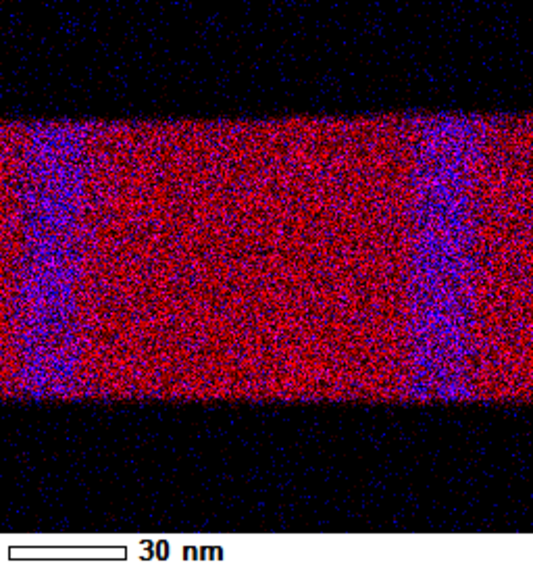
\includegraphics[width=0.48\textwidth]{4_Crystalline_properties/Fig/s4_0deg_IIImap_wells.pdf}
    }
    \subcaptionbox{
        V-element \acs{eds} map. Red \acs{as}, blue \acs{p}
        \label{subfig:s4_0deg_Vmap_wells}
        }{
        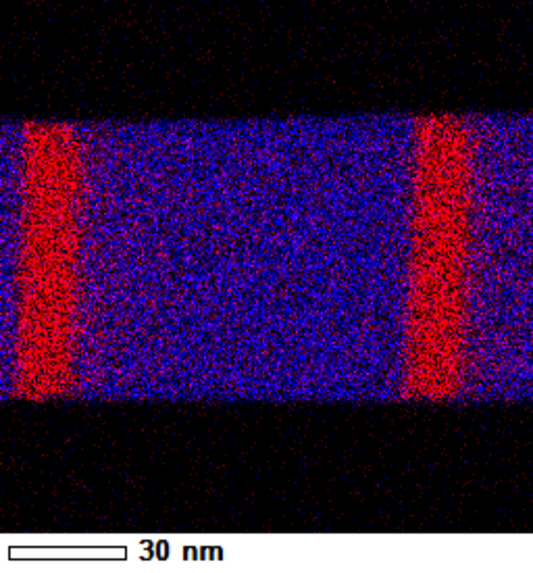
\includegraphics[width=0.48\textwidth]{4_Crystalline_properties/Fig/s4_0deg_Vmap_wells.pdf}
    }
    \caption{\acs{eds} maps of the \acl{qw} region of the \qty{0}{\degree} sample in Figure~\ref{subfig:s4_OV}. The seed is out of frame on the left of the images.}
    \label{fig:s4_0deg_EDS_maps_wells}
\end{figure}

Figure~\ref{fig:s4_0deg_EDS_maps_wells} shows the \acs{eds} maps. The elements \acl{ga} and \acl{p} are colour-coded in blue while \acl{in} and \acl{as} are colour-coded in red. Two \acs{ingaas} \acl{qw}s are visible on both maps, showing the same nanowire area. 

The III-element map shows how \acl{ga} is well-segregated into the \acs{ingaas} layers. However, a difference between the leading and trailing edges of the \acl{qw}s is visible once more when examining the V-element map. Indeed, while the leading edge is sharp, a light red shading is present in the \acl{p} region after the trailing edge. This indicates an \acl{as} contamination in the \acs{inp} barrier layer. As the image is comparable to the one in Figure~\ref{subfig:s3_V_map_wells}, the lengthening of the \acs{p} flow step during the post \acs{ingaas} hold step had a small impact on the resulting post-well composition profile.

\begin{figure}
    \centering
    \subcaptionbox{
    \acs{eds} linescan: III atomic percentage vs position.
    \label{subfig:s4_III_0deg_linesc}
    }{\begin{tikzpicture}
        \begin{axis}[
            width = 0.8\textwidth,
            height = 5cm,
            xlabel = Position (nm),
            ylabel = Composition (atomic \%),
            table/col sep=comma,
            %title = III element composition,
            legend pos=outer north east,
            ymin=0, ymax=100,
            xmin = 0, xmax=230
        ]
    \addplot [cb1_orange,] table[x=nm,y=Ga] {4_Crystalline_properties/csv/s4_III_0deg_linesc.csv};
    \addplot [cb1_dark_blue,] table[x=nm,y=In] {4_Crystalline_properties/csv/s4_III_0deg_linesc.csv};
    \addlegendentry{Ga}
    \addlegendentry{In}
    \end{axis}

    \end{tikzpicture}
    }
    \subcaptionbox{
    \acs{eds} linescan: V atomic percentage vs position.
    \label{subfig:s4_V_0deg_linesc}
    }{\begin{tikzpicture}
        \begin{axis}[
            width = 0.8\textwidth,
            height = 5cm,
            xlabel = Position (nm),
            ylabel = Composition (atomic \%),
            table/col sep=comma,
            %title = V element composition,
            legend pos=outer north east,
            ymin=0, ymax=100,
            xmin = 0, xmax=230
        ]
    \addplot [cb1_orange,] table[x=nm,y=As] {4_Crystalline_properties/csv/s4_V_0deg_linesc.csv};
    \addplot [cb1_dark_blue,] table[x=nm,y=P] {4_Crystalline_properties/csv/s4_V_0deg_linesc.csv};
    \addlegendentry{As}
    \addlegendentry{P}
    \end{axis}

    \end{tikzpicture}
    }
    \caption{\acs{eds} linescan compositional data (in percentage) for the \subref{subfig:s4_III_0deg_linesc} III elements and \subref{subfig:s4_V_0deg_linesc} V elements across all three \acl{qw} of the \qty{0}{\degree} sample seen in Figure~\ref{subfig:s4_OV}. The origin of the x-axis is situated before the first well and is the closest point to the \acs{si} seed. Higher position numbers (in nm) represent the scan moving along the \hkl{1 1 1} vector perpendicular to the growth front away from the seed.}
    \label{fig:s4_0deg_linescans}
\end{figure}

Figure~\ref{fig:s4_0deg_linescans} shows the composition data calculated from the \acs{eds} linescan taken on the \acl{qw} region of the \qty{0}{\degree} sample in Figure~\ref{subfig:s4_OV}. The scan was taken from before the first \acl{qw}, closest to the \acs{si} seed.

The III-element composition profile of Figure~\ref{subfig:s4_III_0deg_linesc} was calculated using the L\(_\alpha\) lines of \acl{in} and \acl{ga}. The graph is very noisy, with noise fluctuations reaching \qty{20}{\%}, but shows a composition close to \ce{In0_.4Ga0_.6As} in all three \acl{qw}s. Similarly to the profile in Figure~\ref{subfig:s3_III_linesc}, suggests the presence of a \acl{ga} composition gradient after the well itself. 

The V-element composition profile of Figure~\ref{subfig:s4_V_0deg_linesc} was calculated using the K\(_\alpha\) lines of \acl{as} and \acl{p}. This graph has noise fluctuations of about \num{10}-\qty{15}{\%}. A \acl{as} percentage composition close to \qty{100}{\%} is present in the \acs{ingaas} \acl{qw} similarly to what was observed for sample 3 (Figure~\ref{subfig:s3_V_linesc}). The \acs{as}-rich region extends for \num{10}-\qty{15}{\nano\metre} after the end of the \acs{ingaas} \acl{qw}.

As the precursor flows were not altered from those of previous samples, the V / III ratios remain as in Table~\ref{tab:sample1_ratios}. The higher concentration of \acl{ga} in the \acl{qw}s could therefore be caused by the change in the geometry of the template given by the difference in device layer thickness of the \hkl<1 1 0> \acs{soi} wafer.

\subsection{Photoluminescence data}

\begin{figure}
    \centering
    \begin{tikzpicture}
        \begin{axis}[
            width = 0.8\textwidth,
            height = 5cm,
            xlabel = Wavelegth (nm),
            ylabel = Intensity (a.u.),
            table/col sep=comma,
            %title = Photoluminescence Spectrum,
            legend pos=outer north east,
            ymin=0, ymax=1000,
            xmin = 1268.8, xmax=1600.3
            ]
            \addplot [cb1_dark_blue,] table[x=wavelength,y=intensity] {4_Crystalline_properties/csv/s4_pl.csv};
            \addlegendentry{Sample 4}
        \end{axis}
    \end{tikzpicture}
    \caption{Photoluminescence spectrum of a nanowire from sample 4. This spectrum was kindly recorded by Markus Scherrer.}
    \label{fig:s4_pl}
\end{figure}

The photoluminescence spectrum in Figure~\ref{fig:s4_pl} was recorded from one of the nanowires in sample 4. The operator selected a nanowire far from parasitic growths. The nanowire was excited with a \qty{1}{\second}-long laser pulse with a wavelength of \qty{1000}{\nano\metre} while cooled to \qty{-200}{\kelvin}. This wavelength was selected as it is higher than the absorption wavelength of \acs{inp} (GET WAVELENGTH) but lower than that of \ce{In0_.53Ga0_.47As} (GET WAVELENGTH). 

As the focus size of a wave is limited by both the diffraction limit and the real (therefore imperfect) optics of the setup, the illumination spot used to excite the nanowire is larger than \qty{500}{\nano\metre} and can be approximated at an order of magnitude of \qty{1}{\micro\metre}. As such, the spot size is much larger than that of even just one of the nanowires, let alone that of the single heterolayers. 

One of the nanowires at the edge of one of the comb structures shown in Figure~\ref{subfig:110_design1} was chosen for measurement to minimise the influence of neighbouring wires as much as possible. The resulting spectrum of Figure~\ref{fig:s4_pl} shows a wide emission range, with an emission peak at the edge of the detector cutoff. The reason for this wide spectrum could lie in the large \acs{ingaas} nucleation layer, which still constitutes the bulk of \acs{ingaas} in the nanowire and grows before the facet stabilisation process mediated by the following \acs{inp} layer.

As such, it becomes important to minimise the length of this nucleation layer as much as possible if the photoluminescence spectrum of the \acs{ingaas} heterostructures is to be recorded.

\section{Minimization of Nucleation Layer Thickness}




\section{Merge Structures}





\section{Growth of Strained Heterolayers}







%\section{article1}
%\begin{figure}
%    \centering
%    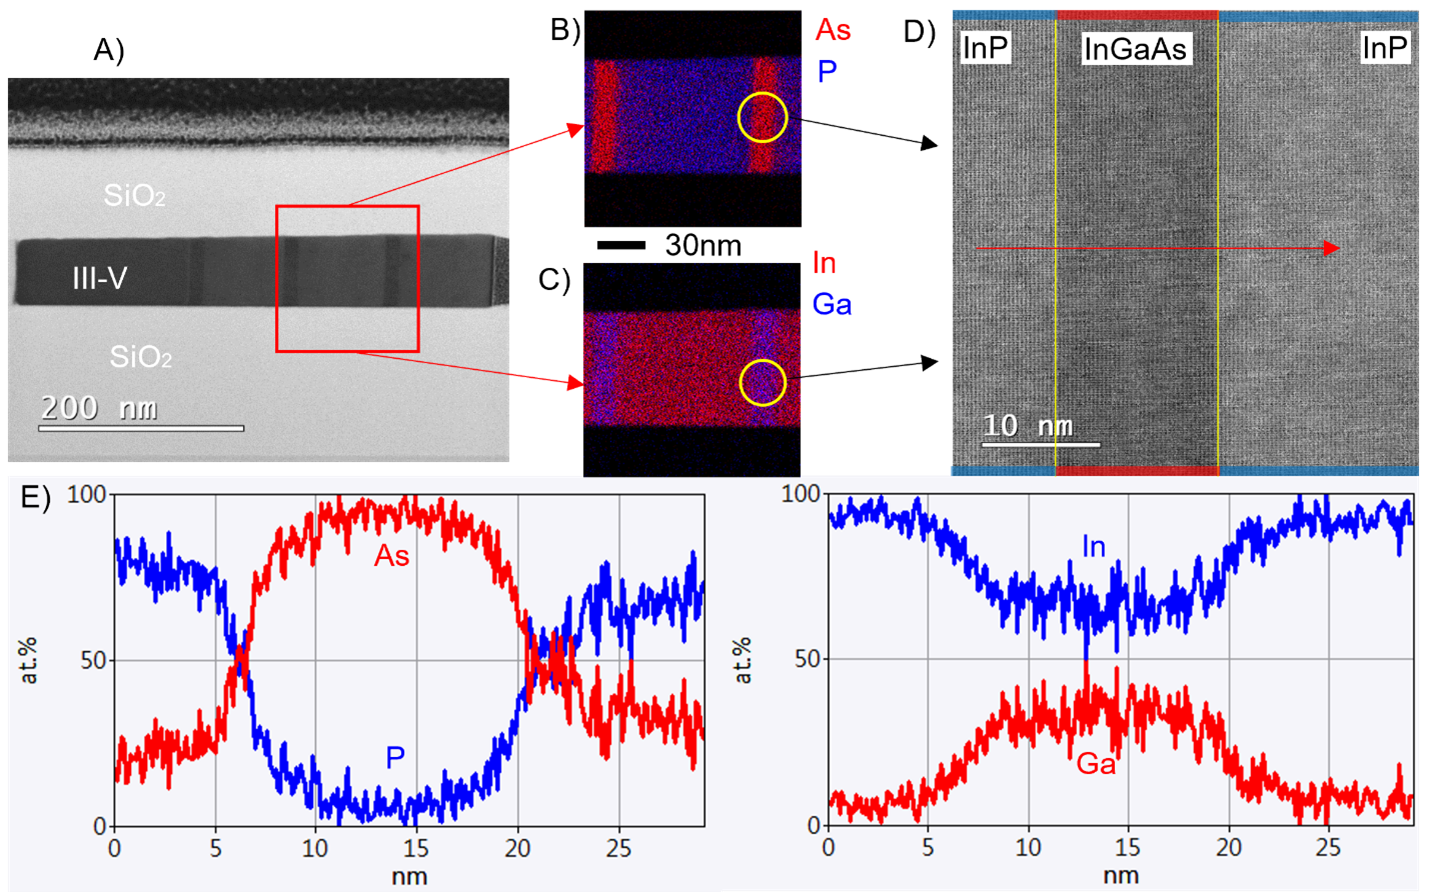
\includegraphics[width=\textwidth]{3_Growth/ICMOVPEXXFig5.png}
%    \caption{STEM image and EDS maps of a lamella cut from one of the nanowires grown on a <110> SOI. A) Overview of the BF-STEM image of the nanowire. The silicon seed is on the left, and silicon oxide is on the top and bottom. The entire heterostructure stack is visible due to channelling contrast: InGaAs appear darker than InP. B) Color-coded EDS map of the region highlighted by the red square in (A): in red In concentration and blue Ga concentration. C) Color-coded EDS map of the region highlighted by the red square in (A): red As concentration and blue P concentration. D) High-resolution BF-STEM detail of the 10-nm-thick InGaAs well. E) EDS line-scan spectra recorded across the InGaAs and highlighted in (D) by the red arrow showing scan direction.}
%    \label{fig:ICMOVPEXXFig5}
%\end{figure}

%In the previous examples, a <001> device layer SOI was used as a growth substrate, where a multi-faceted growth front can develop, leading to poor geometric control, composition variations for ternaries, and in any case, a heterointerface which is not perpendicular to the growth direction, which is an undesirable situation for device fabrication. This can be circumvented using a Si wafer orientation with vertical {111} crystal planes as available on an <110> SOI wafer—

%hfigure 5. A shows a BF-STEM image of a nanowire with vertical and well-defined hetero-interfaces. 

%A similar level of As background impurities is present after each InGaAs segment, as shown in Figure 5. B, while Figure 5. C shows how Ga is well confined to the respective layer. 

%The high-resolution BF-STEM image in Figure 5.D shows the heterointerface between the 85-nm-thick InP on the image's left- and right-hand side and the 14-nm-thick InGaAs quantum well structure that appears as a dark layer in the middle of the image. The extracted <111>B growth rates are 25.5 nm/min for InP and 42.9 nm/min for InGaAs, respectively. This marks an increase in growth rate attributed to the different template shapes, as template height was reduced from 220 nm to 70 nm—

%figure 5. E shows the composition profiles for the III- and group elements across the quantum well region. The presence of As impurities immediately after the quantum well layer is again noticeable on the right side of the V element map, as the As and P concentration profiles are asymmetric. This asymmetry is evident when compared with the symmetric composition profiles for the III-group elements, which maintain the interface quality observed in the sample shown in Figure 4. The III composition profile Figure 5. E highlights how the InxGa1-xAs composition is more prosperous in Indium, having an x = 0.60. As the flows into the reactor were not altered from the sample shown in Figure 4, this composition change can also be attributed to the different template geometry.

\section{article 2}
\begin{figure}
    \centering
    \includegraphics[width=\textwidth]{4_Crystalline_properties/From_Article2/Figure2.png}
    \caption{Top-view SEM images of arrays with grown III-V nanowires. The \qty{70}{\nm}, \qty{140}{\nm}, \qty{210}{\nm}, and \qty{280}{\nm} wide wires are shown from top to bottom. The arrays on the left contain structures grown from a seed surface parallel to the template direction, while those on the right are grown from seed surfaces that are tilted concerning the template. On the bottom left of the images, the three main elements of the arrays are highlighted in green (silicon seed), red (III-V nanowires), and blue (template opening).}
    \label{fig:arrays}
\end{figure}

Figure~\ref{fig:arrays} shows growth results from sample 1 of arrays containing template nanotubes of four different widths (\qty{70}{nm}, \qty{140}{nm}, \qty{210}{nm}, and \qty{280}{nm}). Each array contains 66 nanowires (in red) grown from silicon (in green) and arranged in 33 pairs. Each pair of wires shares the same template opening (in blue). 
\par
Each wire in the array can be identified by its row, opening, and position relative to the latter. Each row is numbered from 1 to 11, starting at the bottom of the array. The template openings are marked by letters A, B, or C; the wires connected to the opening to the left (l) or right (r) can be easily distinguished. Therefore, a string such as 9Br identifies a single wire in the array. 
\par
Our growth methodology aims to select and maintain a single \hkl{111}\(_B\) facet as the nanowire's growth front. If a III-V wire end-surface is multi-faceted or not parallel to the \acs{si} seed facet, the wire is classified as defective in this study without requiring a further in-depth STEM analysis. This first distinction allows the evaluation of the fraction of "perfect" wires, defining a growth yield. 
\par
In Figure~\ref{fig:arrays}, the \qty{280}{nm} tilted arrays present some defective wires in 11Al, 6Cr, and 7Cr; however, the other wires in each pair (11Ar, 6Cl, and 7Cl) appear “perfect”. As is evident in the case of wire 6Cr, the wire grew into an unpredictable shape after nucleation. It is unclear if the source of defective wires can be attributed solely to the nucleation step, as there are other sites (\qty{70}{nm} tilted 6Cl, \qty{140}{nm} perpendicular 2Br, 11Br, and \qty{280}{nm} perpendicular 7Br) that present a defective wire and fully covered seed. However, this finding suggests that nucleation does play an important role in the following growth facet selection.


\begin{figure}
    \centering
    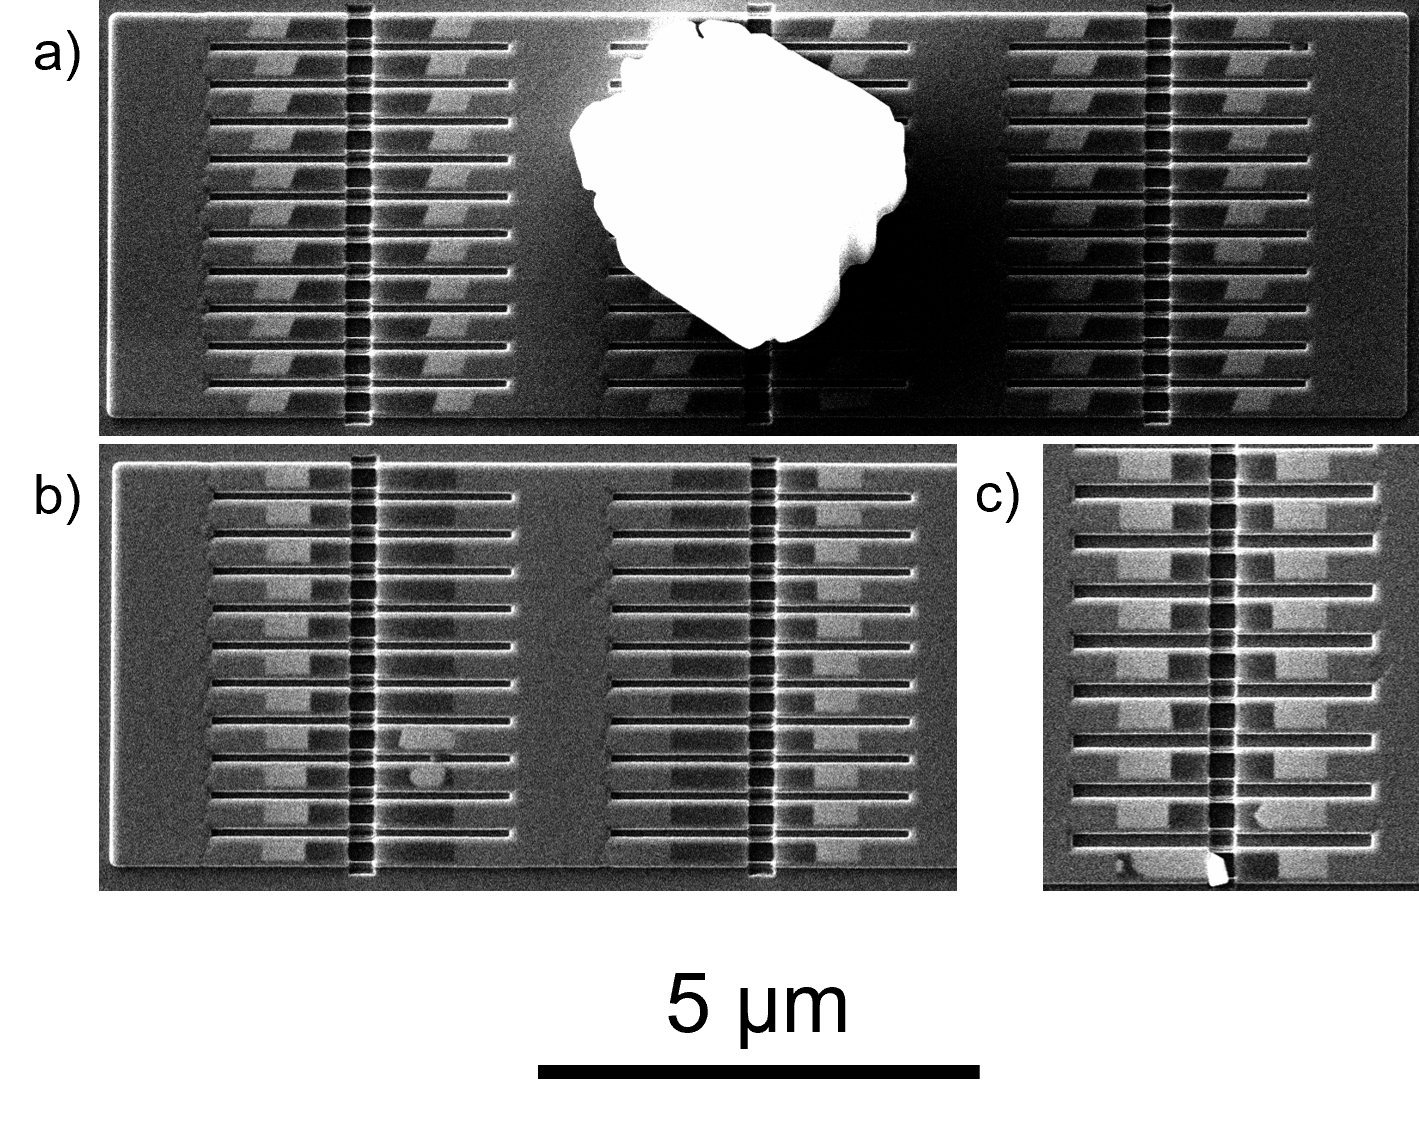
\includegraphics[width=\columnwidth]{4_Crystalline_properties/From_Article2/Figure3.png}
    \caption{Examples of failure situations for TASE grown wires. (a) large parasitic crystal obstructing many growth sites. (b) multiple seeds do not show nucleation of III-V material at all, while one site shows parasitic nucleation inside the template. (c) in the bottom row, after initial nucleation on the \acs{si}, a parasitic crystal developed inside the template and grew out of it.}
    \label{fig:failures}
\end{figure}

Another parameter that negatively affects the growth yield is the loss of growth selectivity and the resulting parasitic growth. This is ascribed to impurities or surface features promoting nucleation. An example of this is shown in Figure~\ref{fig:failures}.a, where a single defect of this kind affects many wires. Figure~\ref{fig:failures}.b also shows sites where parasitic nucleation occurred within templates and, seed-sites that did not undergo III-V on \acs{si} nucleation, likely because of the lingering of a passivating \acs{sio2} layer on the \acs{si} seed surface. This happened despite the proximity to other correctly-grown wires. Finally, 
Figure~\ref{fig:failures}.c bottom row illustrates an example where, after the initial nucleation event, the channel was obstructed by a parasitic nucleation growth within the channel, which extends outside the template. This type of growth configuration can potentially cause deposits similar to that in Figure~\ref{fig:failures}.a.

\subsection{Yield study}

\sisetup{detect-all = true}
\begin{table}
    \centering
    \begin{tabular}{l|ccccccc}
        \hline
         & \multicolumn{7}{c}{Defect categories and occurrence} \\ 
         & $\begin{matrix} \text{Wrong} \\ \text{Facet} \end{matrix}$ & $\begin{matrix} \text{Hidden by} \\ \text{Parasitic} \end{matrix}$ & $\begin{matrix} \text{Oxide} \\ \text{Nucleated} \end{matrix}$ & $\begin{matrix} \text{Seed} \\ \text{Exposed} \end{matrix}$ & Long & Short & Ungrown \\ 
        \hline \hline
         & & & & & & & \\
        Sample 1 & \num{164} & \num{230} & \num{2} & \num{0} & \num{5} & \num{204} & \num{61} \\ 
        \hline
        Parallel & \num{81} & \num{170} & \num{1} & \num{0} & \num{4} & \num{0} & \num{0} \\
        \textit{\% of category} & \textit{\qty{49.4}{\%}} & \textit{\qty{77.9}{\%}} & \textit{\qty{50}{\%}} & \textit{-} & \textit{\qty{80}{\%}} & \textit{\qty{0}{\%}} & \textit{\qty{0}{\%}} \\ 
        \hline
        Tilted & \num{83} & \num{51} & \num{1} & \num{0} & \num{1} & \num{204} & \num{61} \\
        \textit{\% of category} & \textit{\qty{50.6}{\%}} & \textit{\qty{22.1}{\%}} & \textit{\qty{50}{\%}} & \textit{-} & \textit{\qty{20}{\%}} & \textit{\qty{100}{\%}} & \textit{\qty{100}{\%}} \\ 
        \hline
         & & & & & & & \\
        Sample 2 & \num{204} & \num{257} & \num{15} & \num{8} & \num{3} & \num{7} & \num{20} \\ 
        \hline
        Parallel & \num{127} & \num{145} & \num{6} & \num{4} & \num{1} & \num{5} & \num{20} \\
        \textit{\% of category} & \textit{\qty{62.3}{\%}} & \textit{\qty{56.4}{\%}} & \textit{\qty{40}{\%}} & \textit{\qty{50}{\%}} & \textit{\qty{33.3}{\%}} & \textit{\qty{71.4}{\%}} & \textit{\qty{100}{\%}} \\ 
        \hline
        Tilted & \num{77} & \num{112} & \num{9} & \num{4} & \num{2} & \num{2} & \num{0} \\
        \textit{\% of category} & \textit{\qty{37.7}{\%}} & \textit{\qty{43.6}{\%}} & \textit{\qty{60}{\%}} & \textit{\qty{50}{\%}} & \textit{\qty{66.7}{\%}} & \textit{\qty{28.6}{\%}} & \textit{\qty{0}{\%}} \\ 
        \hline
        & & & & & & & \\
        \textbf{Total} & \textbf{\num{368}} & \textbf{\num{487}} & \textbf{\num{17}} & \textbf{\num{8}} & \textbf{\num{8}} & \textbf{\num{211}} & \textbf{\num{81}} \\
        \hline
    \end{tabular}
    \caption{Distribution of failure types for samples 1 and 2. Each sample's total is broken down between wires grown parallel to or tilted away from the \hkl<111> direction. Percentages for these two sub-categories and an overall total are given.}
    \label{tab:failures}
\end{table}
\sisetup{detect-none = true}

A survey of the arrays was carried out using samples 1 and 2, and involved \num{15840} individual nanowires grown in \num{240} arrays grouped in \num{5} locations per sample. The areas investigated were the top left of the chips as well as randomly selected locations throughout it. Wires need to have two parallel visible \hkl{111} seed and end facets of equal length, and they need to have nucleated directly on the \acs{si} seed covering it in its entirety for them to be considered "perfect". Of the \num{15840} total wires \num{14660} match these criteria, totalling a global yield of \qty{92.55}{\%}.
\par
Of the \num{7920} wires imaged for each sample, \num{7254} grew successfully in sample 1, and \num{7406} grew successfully in sample 2, resulting in a corresponding growth yield of \qty{91.59}{\%} and \qty{93.51}{\%}. This result indicates that the different heterointerfaces of samples 1 and 2 do not significantly impact the growth yield. 
\par
Further analysis was carried out within each sample by comparing the template growth yield parallel to the \hkl<111> direction, and those tilted away from it. A larger number (\num{9504} out of \num{15840}) of wires of the first configuration were measured. For sample 2, the parallel and tilted configurations resulted in comparable growth yields of \qty{93.73}{\%} and \qty{93.75}{\%}, while sample 1 showed \qty{94.84}{\%} and \qty{86.71}{\%} growth yields for the same configurations. The larger difference in growth yields for parallel and tilted templates in sample 1 can be explained by one of the fivcategorisedselected locations containing tilted arrays, falling in an area of the chip with many nucleation issues. This area is reflected in Table~\ref{tab:failures} where sample 1 has more short and ungrown wires.
\par
The total of \num{1180} nanowires that experienced growth failure are categorised based on the type of failure they experienced. Table~\ref{tab:failures} breaks down the number of defective wires for each sample between parallel and tilted templates, on a per-category basis. The first category, labelled "wrong facet", groups wires which terminate with either a multi-faceted surface or in a single facet that is not parallel to the seed surface, and accounts for \num{368} wires (\qty{31.2}{\%} of the total defective wires). The second and largest category comprises wire locations hidden by a parasitic crystal (\num{461} wires or \qty{39.0}{\%} of the total failures). From a total of \num{240} arrays, \num{32} are affected by one or more parasitic crystals. Still, the parasitic crystals hide close to \num{15} (\num{14.87} on average) locations for nanowire growth in each of these arrays. The "oxide nucleated" category contains all the cases where a III-V crystal nucleated randomly inside a template instead on the \acs{si} seed and counts \num{17} wires, \qty{1.4}{\%} of the total. The wires in the category "seed exposed" have the expected end facet, but did not fully cover the entire seed surface, leaving some of it exposed (\num{8} wires, \qty{0.7}{\%}). The category "long" comprises wires that were significantly longer than the others but did not have other defects, accounting for \qty{0.7}{\%} of the defective wires for a total of \num{8}. The last two categories are abnormally short wires and ungrown wires, with \num{211} (\qty{20.1}{\%}) and \num{81} (\qty{6.9}{\%}) counts each. These two categories of wires are more common in the area which presented nucleation iCharacterisation1.

\section{Growth rate stability and merging of nanostructures during growth}

\subsection{Heterointerfaces and growth rate in nanowires}

\begin{figure}
    \centering
    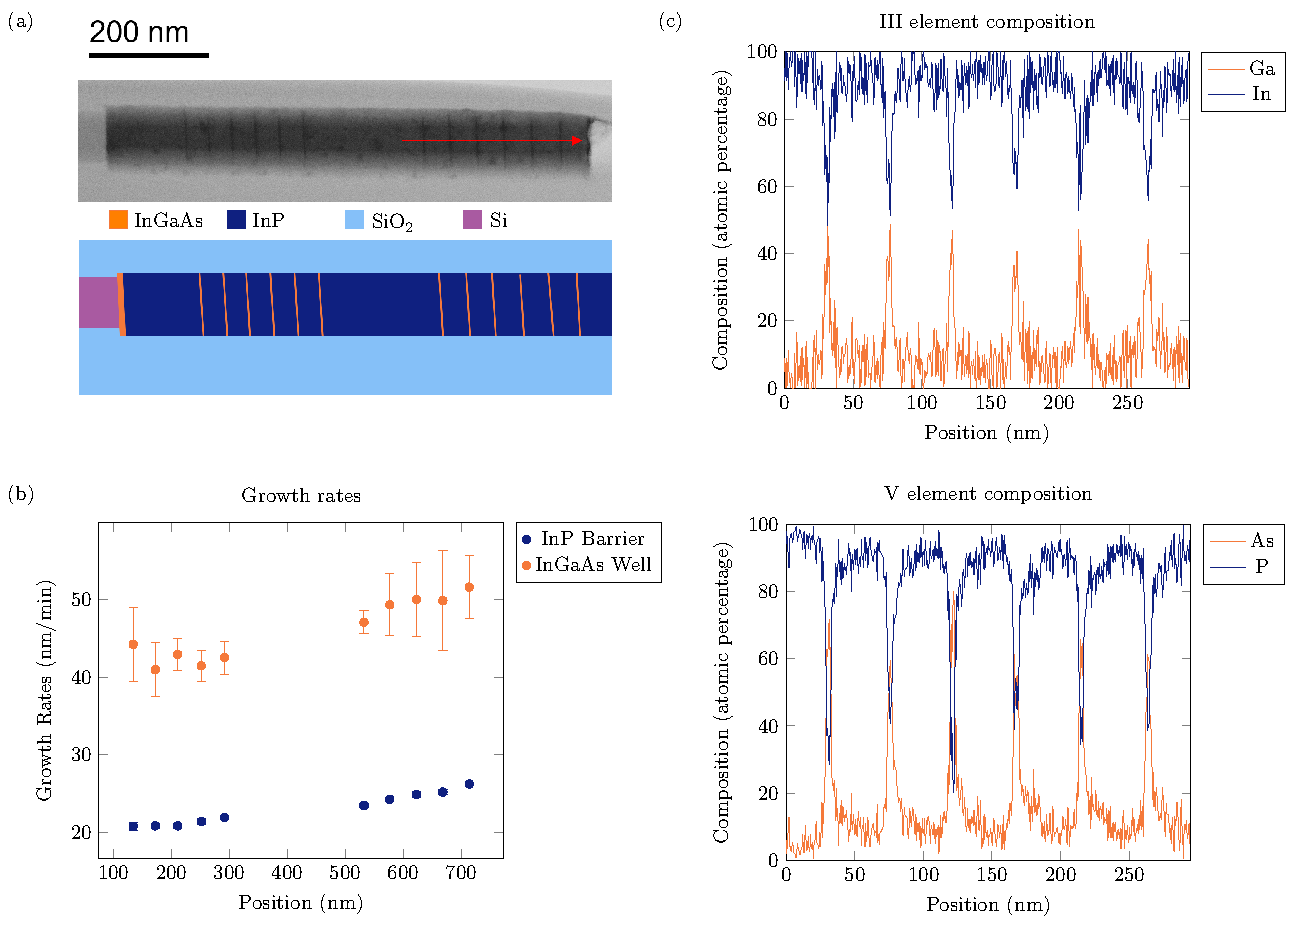
\includegraphics[width=\textwidth]{4_Crystalline_properties/From_Article2/Figure4.pdf}
    \caption{Characterisation results for sample 1. (a) BF-STEM image of the cross-section of one of the nanowires and corresponding schematic composition drawing. (b) growth rates of \acs{ingaas}, in orange, and \acs{inp}, in dark blue. Error bars on all x coordinates, and y coordinates of the \acs{inp} series, are smaller than the graphical markers. (c) composition profiles calculated from an EDS line scan recorded on the location and with the direction marked by the red arrow in (a).}
    \label{fig:growth_rates}
\end{figure}

An in-depth STEM and EDS analysis was carried out to assess the structure of the nanowires. Figure~\ref{fig:growth_rates}.a shows the STEM microscopy image of a FIB cross-section of a wire from sample 1. The blurred regions at the top and bottom are due to the \qty{30}{\degree} cut angle employed to access the \hkl<110> imaging direction. The \qty{4}{\nm} thin, on average, \acs{ingaas} segments are visible as twelve thin dark vertical lines in the dark grey body of the wire. The \acs{ingaas} layers cross-section also act as time markers, recording the morphology of the growth front, and revealing when a single facet is formed and maintained in the growth process. The slight tilt of the heterolayers, which do not appear to be perpendicular to the wafer surface, can partially be explained by a slight tilt of the device \acs{si} layer in this area of the wafer, as well as tilting due to a rotation of the crystalline growth axis during nucleation.
\par
Due to the presence of the \acs{sio2} template, the quantum wells only develop axially and not laterally. This translates into an enhanced composition control in ternary III-V compounds heterolayers incorporated in the nanowires \cite{Borg2019} and therefore is expected to allow for better control of the emission spectra. An EDS line scan of the last six \acs{ingaas} quantum wells was recorded along the direction indicated by the red arrow in Figure~\ref{fig:growth_rates}.a. The resulting composition profiles are shown in Figure~\ref{fig:growth_rates}.c, demonstrating consistent composition profiles across the wells, with the \acs{in} molar fraction being between \num{0.5} and \num{0.6}.
\par
A growth rate analysis is shown in Figure~\ref{fig:growth_rates}.b, revealing a variation in the \acs{inp} growth rate of around \qty{6}{\nm\per\minute} from \qty[separate-uncertainty=true]{20.7 (0.5)}{\nano\metre\per\minute} to \qty[separate-uncertainty=true]{26.2 (0.2)}{\nano\metre\per\minute} along \qty{600}{\nm} of wire. Similarly, a \qty{7}{\nano\metre\per\minute} growth rate increase was recorded for the \acs{ingaas} segments. The error bars represent the \qty{95}{\%} confidence interval on the measurement, calculated by averaging seven thickness measurements taken at various positions for each \acs{inp} and \acs{ingaas} segment. This growth rate increase shows a moderate influence of the diffusional process on the growth dynamics of the samples \cite{bjork2012}.

\begin{figure}
    \centering
    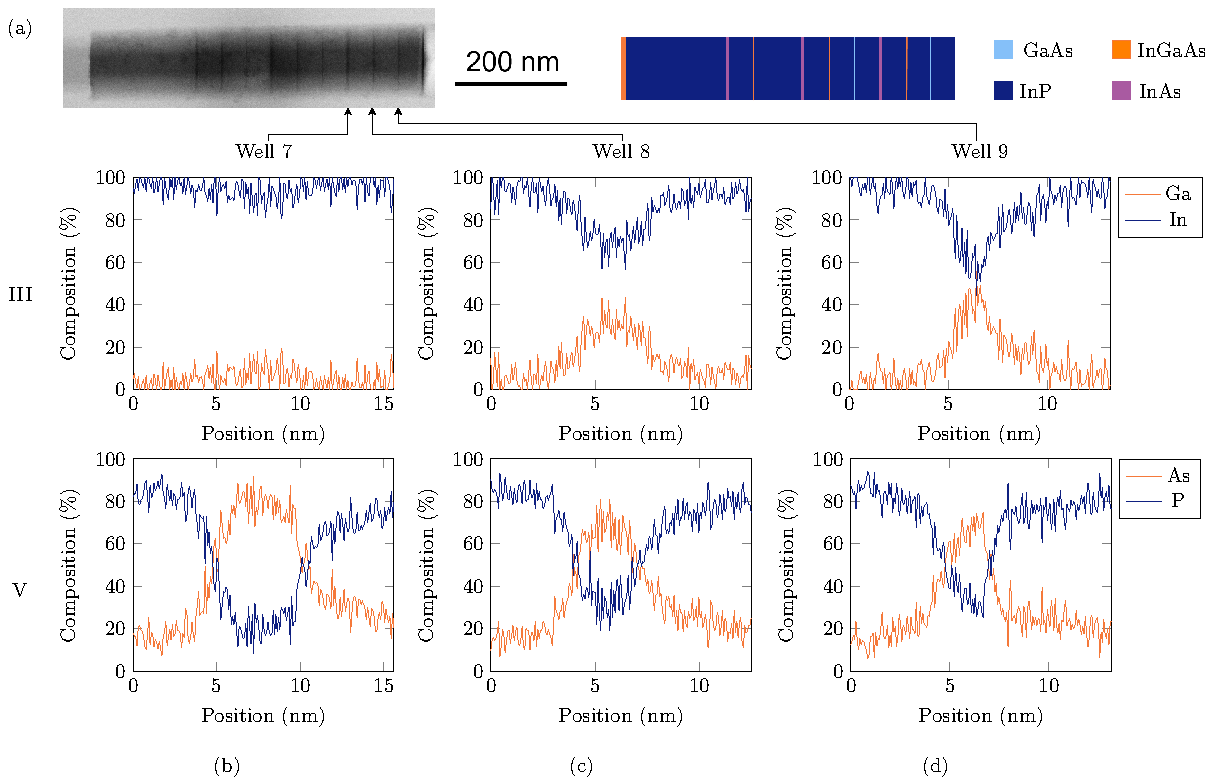
\includegraphics[width=\textwidth]{4_Crystalline_properties/From_Article2/Figure5.pdf}
    \caption{Analysis of sample 2. (a) BF-STEM image of the III-V nanowire, \num{9} lines corresponding to the arsenide layers and corresponding schematic drawing with coloured layers indicating the design composition. Composition profiles for the 7th (b), 8th (c), and 9th (d) wells are calculated from EDS line scans carried out across the respective quantum well from left to right, in the direction parallel to the growth axis.}
    \label{fig:composition}
\end{figure}

A STEM and EDS analysis of sample 2 was conducted to assess the structure and influence of strained heterointerfaces (Figure~\ref{fig:composition}.a) on the growth of nanowires containing three \acs{inp}-\acs{inas}-\acs{inp}-\acs{ingaas}-\acs{inp}-\acs{gaas} heterolayer sequences. Figure~\ref{fig:composition}.b shows the results of the \acs{inas} layer, where only the group V element precursor needs to be switched. The EDS profile indicates that this layer has formed as intended, with a phosphorus background level. 
\par
The \acs{ingaas} segment, with a target composition of \ce{In0_.53Ga0_.47As}, grew \acs{in}-rich, as seen from the EDS profiles in Figure~\ref{fig:composition}.c. A similar observation is made for the intended \acs{gaas} heterostructure: optimisation {fig:composition}.d shows this layer is heavily alloyed with a recorded \acs{in} molar fraction close to \num{0.5}. This indicates that the hold steps implemented in the growth recipe and designed to exhaust the group III element precursor (\acs{in}) were set too short. Further optimisation with prolongation of the purging step is thus suggested to improve composition control for these thin \qty{3}{nm}-wide heterostructures.
\par
The growth rates of the \acs{ingaas} and \acs{inp} layers were assessed with a process analogous to the one used for the growth rates of sample 1. The \acs{inp} growth rates is \qty[separate-uncertainty=true]{23.8 (0.3)}{\nano\metre\per\minute} between the first \acs{inas} and the first \acs{ingaas} wells and \qty[separate-uncertainty=true]{24.0 (0.4)}{\nano\metre\per\minute} between the third \acs{inas} and the third \acs{ingaas} wells. The \acs{ingaas} growth rates are \qty[separate-uncertainty=true]{39 (3)}{\nano\metre\per\minute} for the first \acs{ingaas} well and \qty[separate-uncertainty=true]{44 (2)}{\nano\metre\per\minute} for the third \acs{ingaas} well. All values are averaged from repeated measurements, and errors are given with 95\% certainty. Thus, the growth rates of samples 1 and 2 are comparable for these materials.

\subsection{\texorpdfstring{Growth of wide quantum well structures from multiple \acs{si} seeds}{Growth of wide quantum well structures from multiple Si seeds}}

\begin{figure}
    \centering
    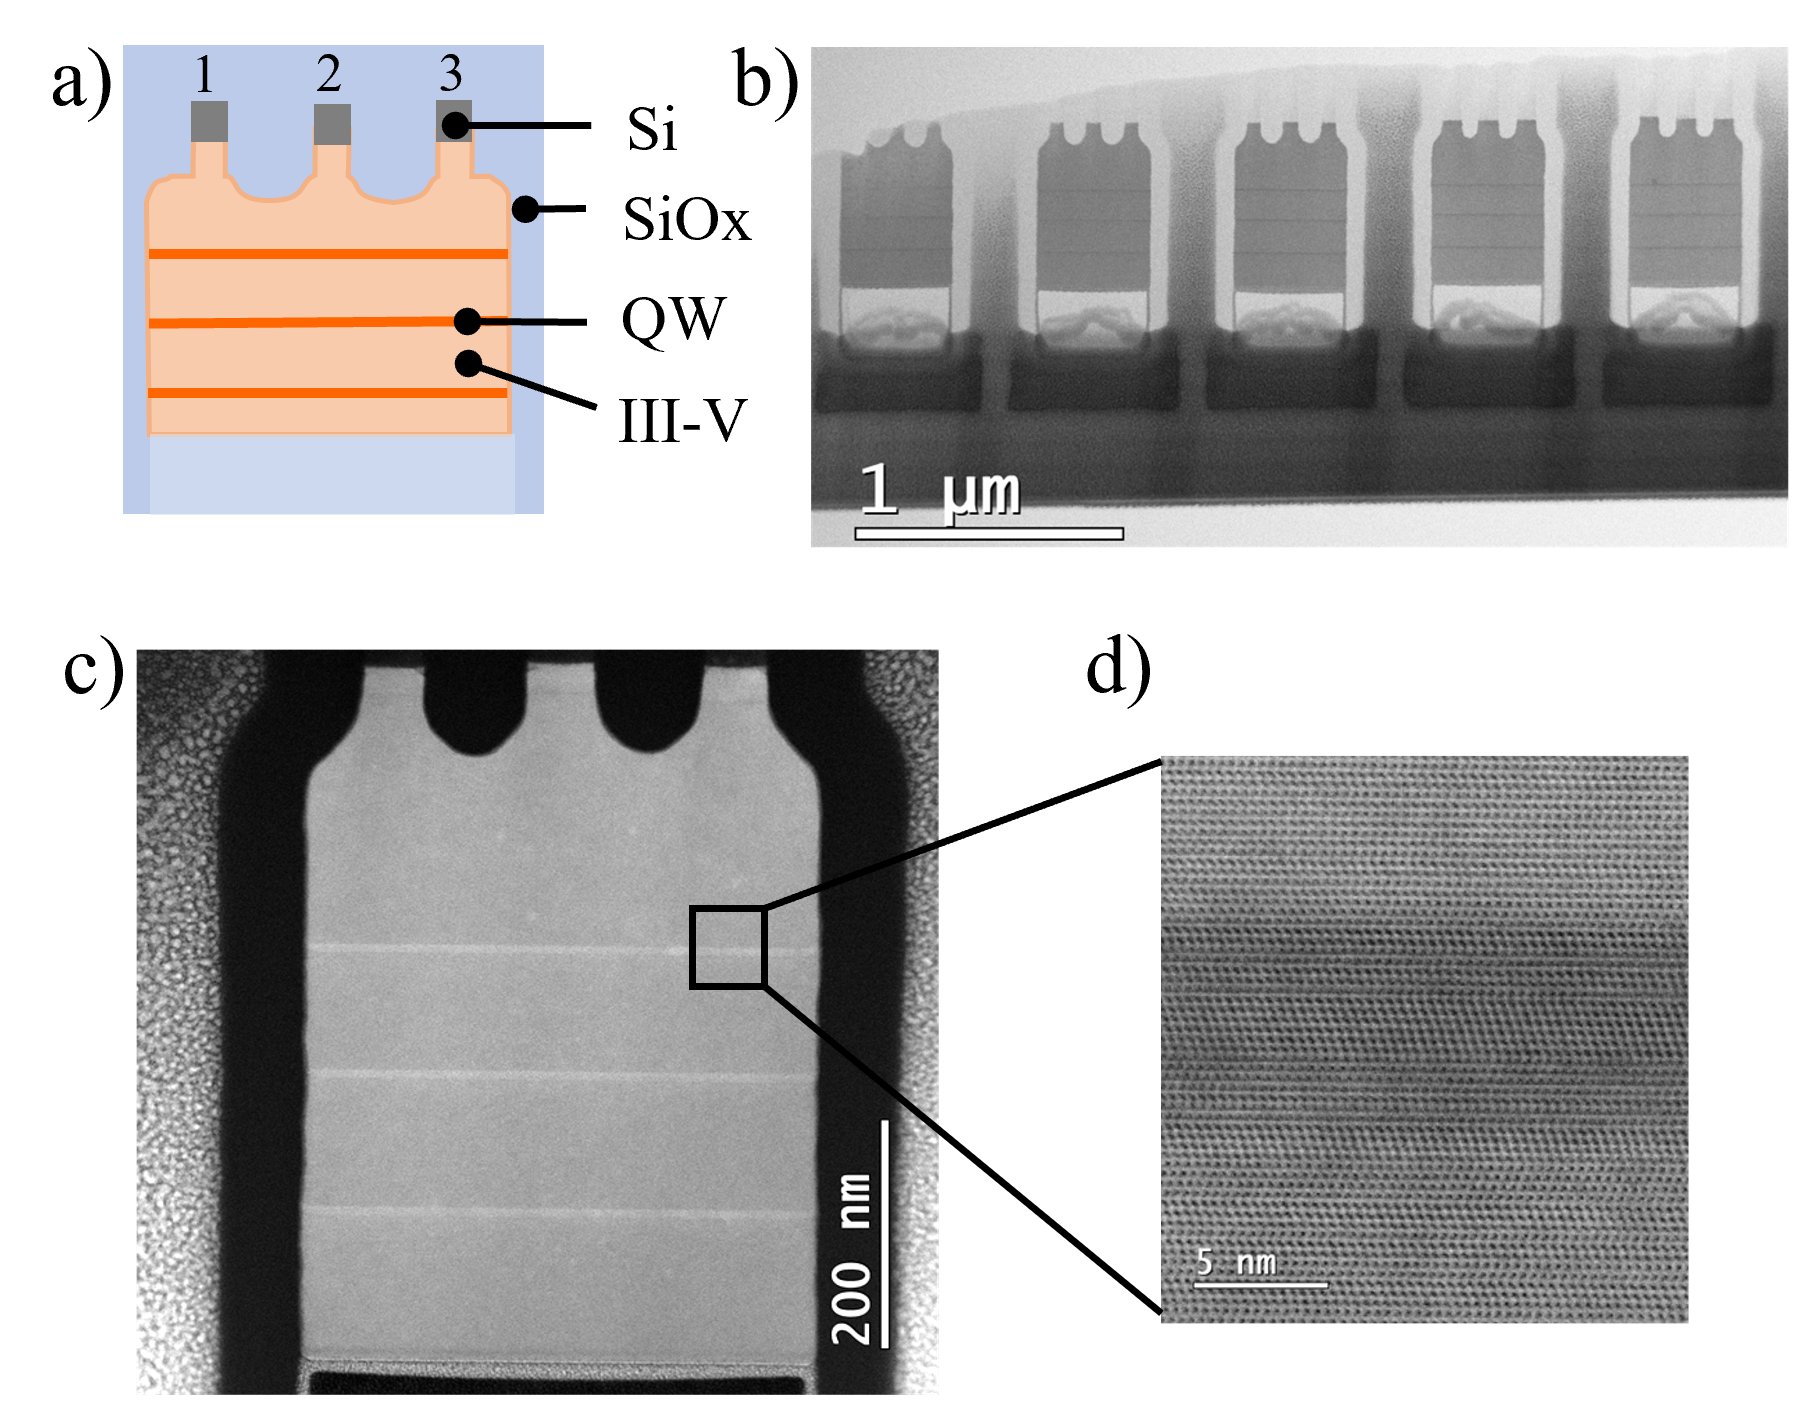
\includegraphics{4_Crystalline_properties/From_Article2/Figure6.png}
    \caption{STEM analysis of quantum wells created in wide structures from the multiple nucleation sites. (a) Top-view schematic of the structure. b) Plane-view image showing five adjacent structures (c) ADF-STEM image of one structure. (d) High-resolution BF-STEM image of a single quantum well.}
    \label{fig:plane_view}
\end{figure}

To demonstrate the robustness of the developed epitaxy process as well as growth recipes, we fabricated test structures of larger width. Furthermore, the template contains not only one \acs{si} nucleation area, but three. Thus the III-V crystal is nucleated in three points simultaneously and develops into short nanowires. These nanowires are then forced to merge into one large platelet of well-defined geometry. The schematic of the structure is illustrated in Figure~\ref{fig:plane_view}.a.
\par
Figure~\ref{fig:plane_view}.b shows a BF-STEM plane-view image of five adjacent structures after STEM lamella preparation. The image shows a high consistency in the overall size of the grown structures and in the presence of the overall \num{15} quantum wells. A single structure is shown in Figure~\ref{fig:plane_view}.c using annular dark field (ADF-)STEM. The three light grey lines correspond to the \acs{ingaas} quantum wells. The high-resolution BF-STEM image in Figure~\ref{fig:plane_view}.d shows one of these quantum wells appearing in darker grey, with additional contrast from alternating stacking sequences forming twin planes which are commonly observed for \hkl<111>\(_B\) growth\cite{Johansson2006}. The quantum well runs uniformly throughout the entire width of the structure, indicating that the growth at this position took place on a single \hkl{111} plane. No other crystal defects were detected in STEM mode. To increase the sensitivity to detect structural defects, standard TEM analysis was performed as well (Figure~\ref{fig:TEM}).

\begin{figure}
    \centering
    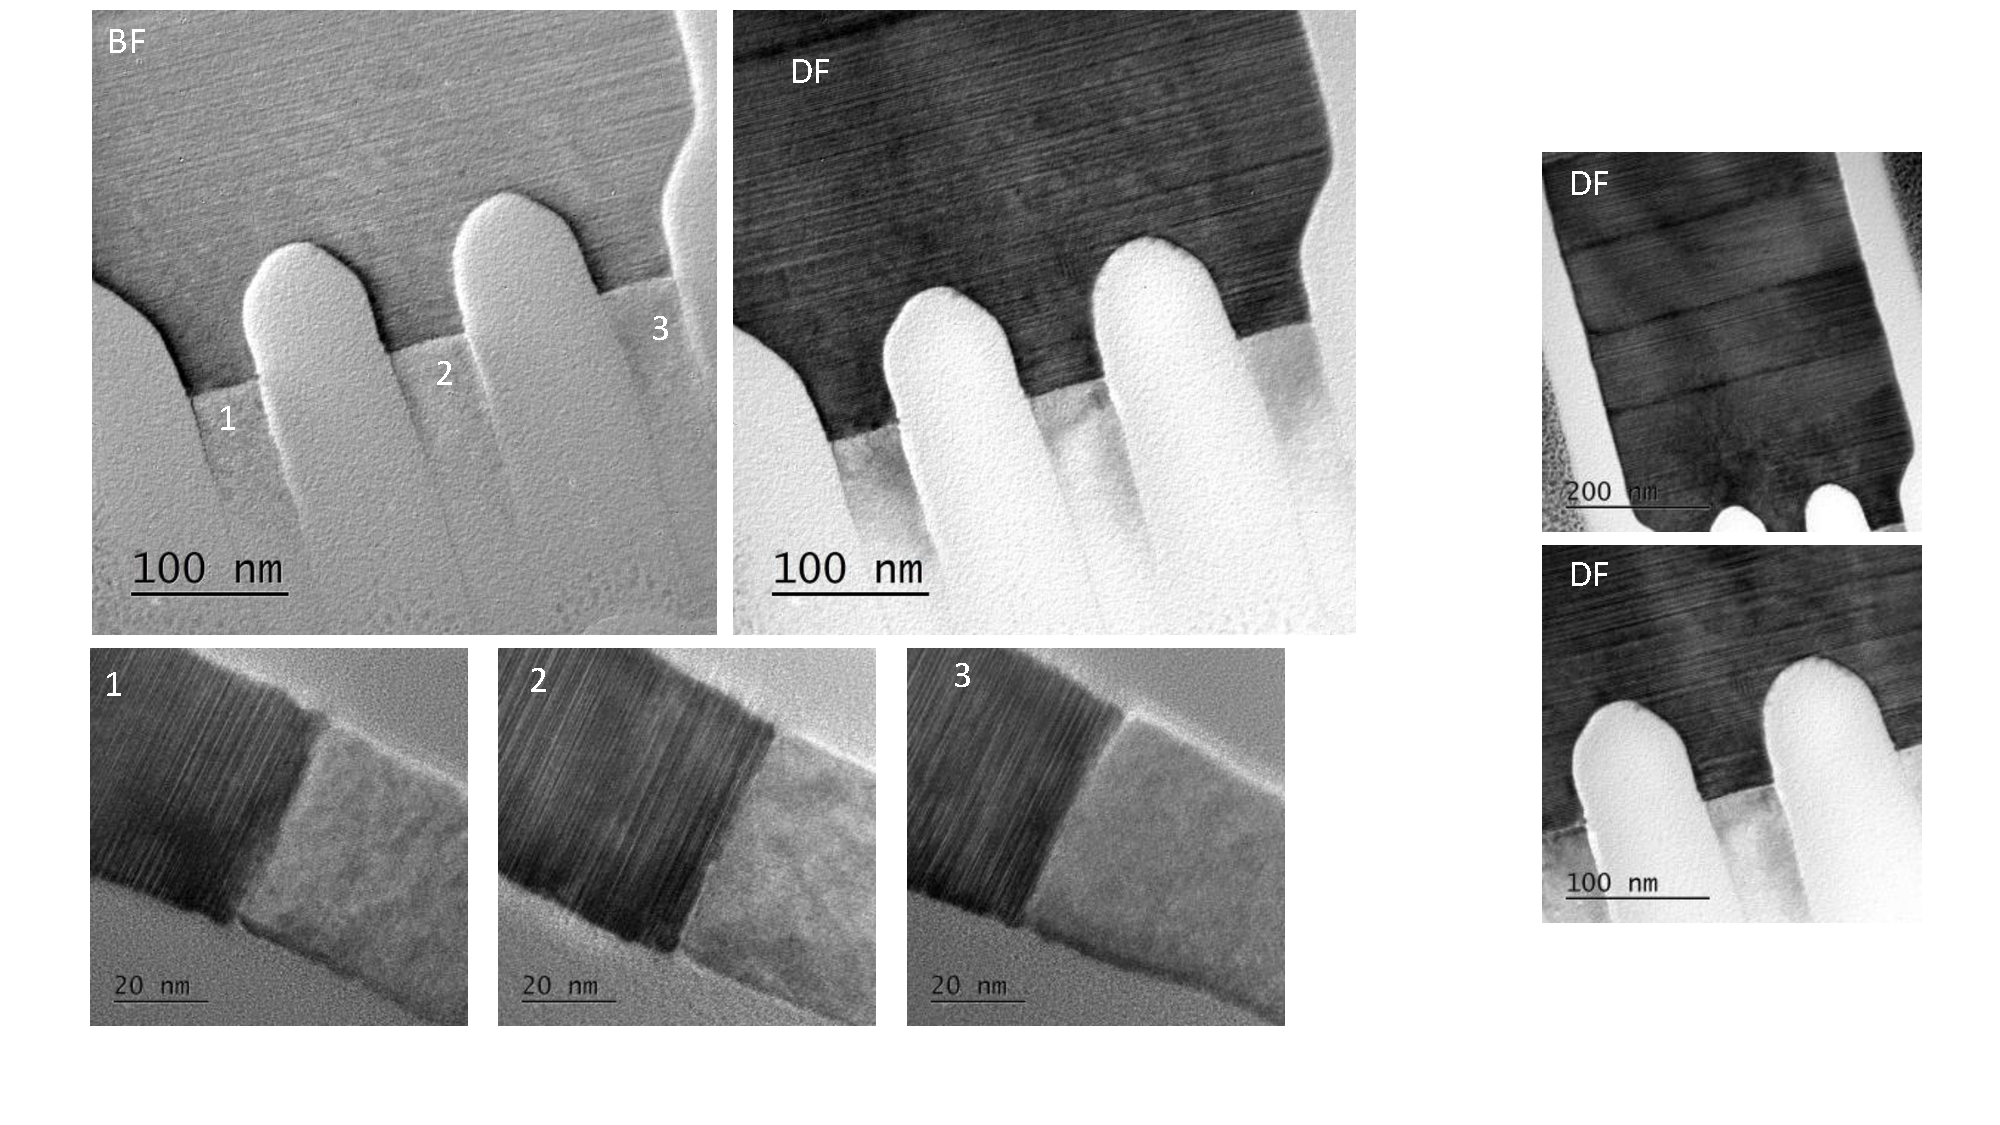
\includegraphics[width = \textwidth]{4_Crystalline_properties/From_Article2/merging_analysis.pdf}
    \caption{TEM analysis of the sampvisualisedFINITIVE FIGURE. PLEASE HEINZ, SEND RAW TEM IMAGES)}
    \label{fig:TEM}
\end{figure}

No propagating dislocations or anti-boundary defects from merging the three initial crystals could be detected. However, this does not exclude the presence of lattice defects which could not be visualised under these imaging conditions. It is unlikely for the three crystal lattices to merge in a perfect registry without the formation of defects\cite{Jacobsson2015, Rossi2023}. However, here the resulting defects remain confined: growth of smooth quantum wells that extend straight across the entire width of the structure would otherwise be impossible.
\par
These observations can be explained by the specific sample geometry, growth directions, and material properties involved. The experiment is arranged in such a way that a \hkl{111} growth front dominates, and no other growth planes are formed. This is achieved by setting a growth condition favouring slow growth along the main \hkl<111> direction and fast growth in the \hkl<110> directions. Under these conditions, efficient step flow occurs on the \hkl{111} facets. In such a configuration, the first wire to extend into the widening template section would spill over the spacre-stabilisesg it from the neighbouring wires and find itself supported on the other wire's \hkl{111} surface. Due to the efficient step flow on the \hkl{111} facets, mismatches of a few monolayers among the three wires are quickly resolved by the formation of one large growth surface that re-stabilises a single \hkl{111} growth front. A single crystal is established beyond these merging points, and growth can extend further into the template cavity.
\par
These structures share strong indications of local growth rate uniformity and simultaneous nucleation. The \num{5.7} width-to-height aspect ratio of the design \qtyproduct{400 x 70}{nm} cross-section is higher than the \num{5} width-to-height aspect ratio (\qtyproduct{3000 x 500}{nm} cross-section) used by \citeauthor{Han2020} and shows a marked improvement in the control of shape and thickness of internal heterostructures. Further, our growth (carried out at \qty{580}{\degreeCelsius}) results are consistent with those obtained homoepitaxially at \qty{570}{\degreeCelsius} with a width-to-height cross-section of \num{20} by \citeauthor{Goswami2020}.
%\chapter{Growth Yield Analysis}
\label{chap:ml}

\section{article2}
\begin{figure}
    \centering
    \includegraphics[width=\textwidth]{4_Crystalline_properties/From_Article2/Figure2.png}
    \caption{Top-view SEM images of arrays with grown III-V nanowires. The \qty{70}{\nm}, \qty{140}{\nm}, \qty{210}{\nm}, and \qty{280}{\nm} wide wires are shown from top to bottom. The arrays on the left contain structures grown from a seed surface parallel to the template direction, while those on the right are grown from seed surfaces that are tilted concerning the template. On the bottom left of the images, the three main elements of the arrays are highlighted in green (silicon seed), red (III-V nanowires), and blue (template opening).}
    \label{fig:arrays}
\end{figure}

Figure~\ref{fig:arrays} shows growth results from sample 1 of arrays containing template nanotubes of four different widths (\qty{70}{nm}, \qty{140}{nm}, \qty{210}{nm}, and \qty{280}{nm}). Each array contains 66 nanowires (in red) grown from silicon (in green) and arranged in 33 pairs. Each pair of wires shares the same template opening (in blue). 
\par
Each wire in the array can be identified by its row, opening, and position relative to the latter. Each row is numbered from 1 to 11, starting at the bottom of the array. The template openings are marked by letters A, B, or C; the wires connected to the opening to the left (l) or right (r) can be easily distinguished. Therefore, a string such as 9Br identifies a single wire in the array. 
\par
Our growth methodology aims to select and maintain a single \hkl{111}\(_B\) facet as the nanowire's growth front. If a III-V wire end-surface is multi-faceted or not parallel to the \acs{si} seed facet, the wire is classified as defective in this study without requiring a further in-depth STEM analysis. This first distinction allows the evaluation of the fraction of "perfect" wires, defining a growth yield. 
\par
In Figure~\ref{fig:arrays}, the \qty{280}{nm} tilted arrays present some defective wires in 11Al, 6Cr, and 7Cr; however, the other wires in each pair (11Ar, 6Cl, and 7Cl) appear “perfect”. As is evident in the case of wire 6Cr, the wire grew into an unpredictable shape after nucleation. It is unclear if the source of defective wires can be attributed solely to the nucleation step, as there are other sites (\qty{70}{nm} tilted 6Cl, \qty{140}{nm} perpendicular 2Br, 11Br, and \qty{280}{nm} perpendicular 7Br) that present a defective wire and fully covered seed. However, this finding suggests that nucleation does play an important role in the following growth facet selection.


\begin{figure}
    \centering
    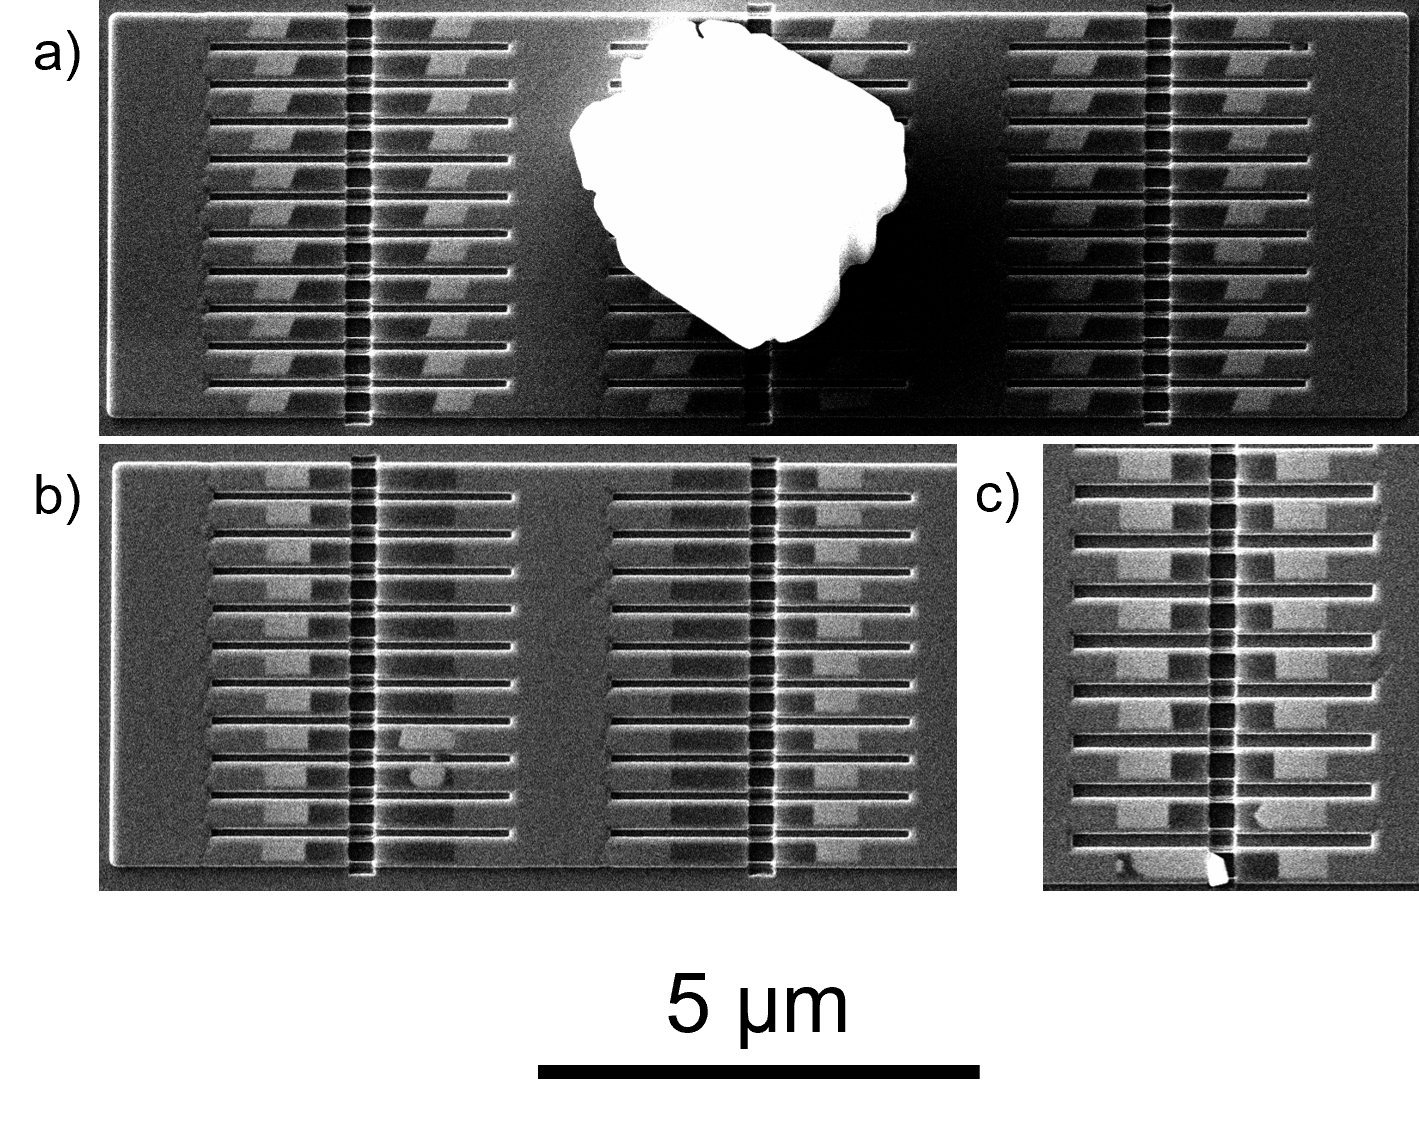
\includegraphics[width=\columnwidth]{4_Crystalline_properties/From_Article2/Figure3.png}
    \caption{Examples of failure situations for TASE grown wires. (a) large parasitic crystal obstructing many growth sites. (b) multiple seeds do not show nucleation of III-V material at all, while one site shows parasitic nucleation inside the template. (c) in the bottom row, after initial nucleation on the \acs{si}, a parasitic crystal developed inside the template and grew out of it.}
    \label{fig:failures}
\end{figure}

Another parameter that negatively affects the growth yield is the loss of growth selectivity and the resulting parasitic growth. This is ascribed to impurities or surface features promoting nucleation. An example of this is shown in Figure~\ref{fig:failures}.a, where a single defect of this kind affects many wires. Figure~\ref{fig:failures}.b also shows sites where parasitic nucleation occurred within templates and, seed-sites that did not undergo III-V on \acs{si} nucleation, likely because of the lingering of a passivating \acs{sio2} layer on the \acs{si} seed surface. This happened despite the proximity to other correctly-grown wires. Finally, 
Figure~\ref{fig:failures}.c bottom row illustrates an example where, after the initial nucleation event, the channel was obstructed by a parasitic nucleation growth within the channel, which extends outside the template. This type of growth configuration can potentially cause deposits similar to that in Figure~\ref{fig:failures}.a.

\subsection{Yield study}

\sisetup{detect-all = true}
\begin{table}
    \centering
    \begin{tabular}{l|ccccccc}
        \hline
         & \multicolumn{7}{c}{Defect categories and occurrence} \\ 
         & $\begin{matrix} \text{Wrong} \\ \text{Facet} \end{matrix}$ & $\begin{matrix} \text{Hidden by} \\ \text{Parasitic} \end{matrix}$ & $\begin{matrix} \text{Oxide} \\ \text{Nucleated} \end{matrix}$ & $\begin{matrix} \text{Seed} \\ \text{Exposed} \end{matrix}$ & Long & Short & Ungrown \\ 
        \hline \hline
         & & & & & & & \\
        Sample 1 & \num{164} & \num{230} & \num{2} & \num{0} & \num{5} & \num{204} & \num{61} \\ 
        \hline
        Parallel & \num{81} & \num{170} & \num{1} & \num{0} & \num{4} & \num{0} & \num{0} \\
        \textit{\% of category} & \textit{\qty{49.4}{\%}} & \textit{\qty{77.9}{\%}} & \textit{\qty{50}{\%}} & \textit{-} & \textit{\qty{80}{\%}} & \textit{\qty{0}{\%}} & \textit{\qty{0}{\%}} \\ 
        \hline
        Tilted & \num{83} & \num{51} & \num{1} & \num{0} & \num{1} & \num{204} & \num{61} \\
        \textit{\% of category} & \textit{\qty{50.6}{\%}} & \textit{\qty{22.1}{\%}} & \textit{\qty{50}{\%}} & \textit{-} & \textit{\qty{20}{\%}} & \textit{\qty{100}{\%}} & \textit{\qty{100}{\%}} \\ 
        \hline
         & & & & & & & \\
        Sample 2 & \num{204} & \num{257} & \num{15} & \num{8} & \num{3} & \num{7} & \num{20} \\ 
        \hline
        Parallel & \num{127} & \num{145} & \num{6} & \num{4} & \num{1} & \num{5} & \num{20} \\
        \textit{\% of category} & \textit{\qty{62.3}{\%}} & \textit{\qty{56.4}{\%}} & \textit{\qty{40}{\%}} & \textit{\qty{50}{\%}} & \textit{\qty{33.3}{\%}} & \textit{\qty{71.4}{\%}} & \textit{\qty{100}{\%}} \\ 
        \hline
        Tilted & \num{77} & \num{112} & \num{9} & \num{4} & \num{2} & \num{2} & \num{0} \\
        \textit{\% of category} & \textit{\qty{37.7}{\%}} & \textit{\qty{43.6}{\%}} & \textit{\qty{60}{\%}} & \textit{\qty{50}{\%}} & \textit{\qty{66.7}{\%}} & \textit{\qty{28.6}{\%}} & \textit{\qty{0}{\%}} \\ 
        \hline
        & & & & & & & \\
        \textbf{Total} & \textbf{\num{368}} & \textbf{\num{487}} & \textbf{\num{17}} & \textbf{\num{8}} & \textbf{\num{8}} & \textbf{\num{211}} & \textbf{\num{81}} \\
        \hline
    \end{tabular}
    \caption{Distribution of failure types for samples 1 and 2. Each sample's total is broken down between wires grown parallel to or tilted away from the \hkl<111> direction. Percentages for these two sub-categories and an overall total are given.}
    \label{tab:failures}
\end{table}
\sisetup{detect-none = true}

A survey of the arrays was carried out using samples 1 and 2, and involved \num{15840} individual nanowires grown in \num{240} arrays grouped in \num{5} locations per sample. The areas investigated were the top left of the chips as well as randomly selected locations throughout it. Wires need to have two parallel visible \hkl{111} seed and end facets of equal length, and they need to have nucleated directly on the \acs{si} seed covering it in its entirety for them to be considered "perfect". Of the \num{15840} total wires \num{14660} match these criteria, totalling a global yield of \qty{92.55}{\%}.
\par
Of the \num{7920} wires imaged for each sample, \num{7254} grew successfully in sample 1, and \num{7406} grew successfully in sample 2, resulting in a corresponding growth yield of \qty{91.59}{\%} and \qty{93.51}{\%}. This result indicates that the different heterointerfaces of samples 1 and 2 do not significantly impact the growth yield. 
\par
Further analysis was carried out within each sample by comparing the template growth yield parallel to the \hkl<111> direction, and those tilted away from it. A larger number (\num{9504} out of \num{15840}) of wires of the first configuration were measured. For sample 2, the parallel and tilted configurations resulted in comparable growth yields of \qty{93.73}{\%} and \qty{93.75}{\%}, while sample 1 showed \qty{94.84}{\%} and \qty{86.71}{\%} growth yields for the same configurations. The larger difference in growth yields for parallel and tilted templates in sample 1 can be explained by one of the fivcategorisedselected locations containing tilted arrays, falling in an area of the chip with many nucleation issues. This area is reflected in Table~\ref{tab:failures} where sample 1 has more short and ungrown wires.
\par
The total of \num{1180} nanowires that experienced growth failure are categorised based on the type of failure they experienced. Table~\ref{tab:failures} breaks down the number of defective wires for each sample between parallel and tilted templates, on a per-category basis. The first category, labelled "wrong facet", groups wires which terminate with either a multi-faceted surface or in a single facet that is not parallel to the seed surface, and accounts for \num{368} wires (\qty{31.2}{\%} of the total defective wires). The second and largest category comprises wire locations hidden by a parasitic crystal (\num{461} wires or \qty{39.0}{\%} of the total failures). From a total of \num{240} arrays, \num{32} are affected by one or more parasitic crystals. Still, the parasitic crystals hide close to \num{15} (\num{14.87} on average) locations for nanowire growth in each of these arrays. The "oxide nucleated" category contains all the cases where a III-V crystal nucleated randomly inside a template instead on the \acs{si} seed and counts \num{17} wires, \qty{1.4}{\%} of the total. The wires in the category "seed exposed" have the expected end facet, but did not fully cover the entire seed surface, leaving some of it exposed (\num{8} wires, \qty{0.7}{\%}). The category "long" comprises wires that were significantly longer than the others but did not have other defects, accounting for \qty{0.7}{\%} of the defective wires for a total of \num{8}. The last two categories are abnormally short wires and ungrown wires, with \num{211} (\qty{20.1}{\%}) and \num{81} (\qty{6.9}{\%}) counts each. These two categories of wires are more common in the area which presented nucleation iCharacterisation1.
%\chapter{Conclusions}
\label{chap:conclusions}

The work presented in this thesis focused on the identification of the conditions under which the \acf{mocvd} of III-V semiconductors in \acf{tase} templates results in a growth front consisting of a single \hkl{1 1 1}\(_B\) facet, the integration of thin heterostructures capable of quantum confinement in a \acs{tase} nanowire, the properties of the nanowires grown with this method, and its yield. The study initially only focussed on the lattice matched \ce{In0_.55Ga0_.45As} and \acs{inp} semiconductors.

The process began by analysing a single heterostructure consisting of two material segments, which showed the difference in growth front morphology between \acf{ingaas} grown with a low V / III ratio and \acf{inp} grown with a high V / III ratio. As seen in Figure~\ref{subfig:sample1_cross-sec}, the low V / III \acs{ingaas} layer grew with the arrowhead growth front, well known in literature \cite{Knoedler2017}, consisting of two \hkl{1 1 0} faces on the upper half of the wire and a \hkl{1 1 1} facet at the bottom. Conversely, in the high V / III ratio \acs{inp} segment the growth rate was increased along the \hkl{1 1 0} directions, resulting in the annihilation of the two top \hkl{1 1 0} facets to the benefit of the bottom \hkl{1 1 1} facet. Therefore, it became clear that a high V / III ratio \acs{inp} growth regimen achieves the goal of stabilising the single-facet growth front.

However, when quick switching between precursors was attempted to create a thin heterostructure, the resulting nanowire, seen in Figure~\ref{fig:sample2_stem}, showed a high composition of elements of the III group intermixing in the heterointerfaces coupled with the integration delay between elements of the III and V group. This caused the III and V concentration gradients to be misaligned. However, the V group element \acf{eds} map also showed potential for well-defined quantum confinement structures.

Some recipe adjustments were made to build on the stabilisation of the \hkl{1 1 1} facet shown to occur in \acs{inp} growth with high V / III ratios, solve III - V integration delay, and improve III group element definition at the heterointerface. The introduction of hold steps in the recipe was shown to achieve all of these objectives in Figure~\ref{fig:s3_ov}. Later experiments showed that increasing the length of the \acs{inp} stabilisation segment and reducing the deposition time of the \acs{ingaas} nucleation layer reduced variability in the stabilisation results. This created a platform allowing for consistent III group element integration across the entire growth front and for constant growth rates, simplifying layer thickness control in quantum confinement structures.

Which of the two available \hkl{1 1 1} facets would stabilise as a growth front in the \hkl(0 0 1) \acf{soi} wafer remained, however, a stochastic problem. A switch to a \hkl(1 1 0) \acs{soi} wafer was made to allow for a consistent selection of best aligned \hkl{1 1 1} in-plane facet. For comparison, the device layer \acs{si} of the \hkl(0 0 1) wafer was \qty{220}{\nano\metre} thick, while the new \hkl(1 1 0) wafer had a device layer thickness of \qty{70}{\nano\metre}. As the device layer's thickness determines the nanostructures' height, the new nanowires' growth rates changed slightly compared to those of the old nanowires but remained comparable.

Growth in a competitive environment was studied on an area of the chip with diffused parasitic nucleation. Here, the nanowires competed with each other, but also with crystals unconstricted by the \acs{tase} template. The presence of these crystals, which acted as larger and larger capture centers for precursors as their surface area grew, changed the effective V / III ratio inside the \acs{tase} template. As a result, the growth rates of each consecutive material layer started to diminish despite the growth front progressing towards the template opening - a situation which was accompanied by a growth rate increase in previous nanowires. Finally, even the stabilising effect given by the high V / III ratio broke down and a multi-faceted growth front was re-established. This effect should be accounted for in the growth of dense sets of \acs{tase} structures with different shapes.

The \hkl{1 1 1}\(_B\) stabilisation method proved to be an exciting avenue to grow defect-free single crystals from simultaneous nucleation on multiple seeds, as shown in Figure~\ref{fig:merge_ov}. The defect-free merging of the three seed crystals was achieved thanks to the layer-by-layer growth on \hkl{1 1 1} atomic planes enabled by the highly controlled growth regimen established during the deposition of \acs{inp} with a high V / III ratio.

The deposition of \acs{ingaas} layers with a thickness of four atomic bi-layers was an achievement at the very limit of what can be achieved with \acf{mocvd}, highlighting both the merits and limitations of the recipe developed in this thesis. It also showed how any heterointerface achievable with this method is finite with a width larger than \qty{2}{\nano\metre}.

The deposition of lattice mismatched \acf{inas} between 

\section{Future Directions}

can address twinning (already have ref of twin free growth on 111)

can select 110 by using a method similar to goswami et al (first go up and then laterally) with a si (110) soi

further fib-sem study on etch-back and relation of seed shape to growth front morfology (among other things, can you eliminate the 2 possibilities of the (1 1 1) facet on (0 0 1) soi by changing the seed shape?)

thickness limit (and as a function of how much the facet is stabilised)


\section{old conclusions}

\subsection{growth}

The main accomplishment in this chapter was the identification and exploitation of the high V/III ratio \acs{inp} \acs{mocvd} growth conditions' effect on the stabilisation of the \hkl{1 1 1}\(_B\) facet as the single growth front for the growing III-V nanowire. This avoids issues related to different incorporation rates of III-elements in ternary materials such as \acs{ingaas} \cite{Borg2019} and creates compositionally uniform material layers. This is then united with the introduction of hold steps, which mitigate the effect of the adsorbate diffusion pathway, avoiding creating a reservoir effect for the III-component, which are integrated into their design layer as expected and without delay. 

This is expected to provide a solution or, at the very least, improve on all of the issues identified in Figure~\ref{fig:wen}. However, some critical problems remain. The first is related to the possibility of the stabilisation of either of 2 different \hkl{1 1 1} facets. This negates the advantage gained in terms of contact positioning, as the selection of the \hkl{1 1 1} facet remains a stochastic process. This is an unsolvable problem with the \hkl[0 0 1] \acs{soi} wafer, as this substrate defines the crystalline orientation of the growing wire. 

As the experiments described on this sample were being carried out, Markus F. Ritter was in the process of publishing a paper on hybrid \acs{tase}, a methodology through which part of the \acs{sio2} template is switched out for a superconducting material \cite{Ritter2021}. As a result of a collaboration on the \acs{stem_m} analysis of hybrid \acs{tase} samples, access to \hkl[1 1 0] \acs{soi} wafers as a growth substrate was obtained for this project. This new crystalline orientation of the growth substrate means that there are in-plane \hkl<1 1 1> vectors at high angles with respect to each other, and prompted my interest in using these wafers as the substrate for the next steps of my research.

This new wafer had a \acs{si} device layer thickness of \qty{70}{\nano\metre} and a \qty{220}{\nano\metre}-thick buried oxide layer, compared to the \hkl[0 0 1] wafer employed so far for which the thicknesses were \qty{220}{\nano\metre} and \qty{2}{\micro\metre}, respectively. The new wafer, therefore, is less suited for optoelectronic and photonic applications but should still prove an ideal test bed for the study of \acs{mocvd} growth dynamics.

In particular, there are remaining questions on the reproducibility of the study, the yield of the growth stabilization, the optical properties of the devices and the application of this facet stabilization method to the integration of different III-V materials outside of the lattice-matched \ce{In0_.55Ga0_.45As} and \acs{inp} material system \cite{Pearsall1980, Sugii1983, Wagner1970} studied in this chapter.

\subsection{properties}

This chapter explored a variety of \acs{mocvd}-grown \acs{tase} structures with various layer thicknesses and semiconductor materials. The \hkl{1 1 1} single growth front stabilisation growth regimen was confirmed to be an attractive methodology for controlling defects and material composition. Initially limited to a high V-III ratio \acs{inp}, it was shown that a high V-III ratio \ce{InAsP} can also provide the same \hkl{1 1 1} stabilisation effect. 

This growth methodology was easy to apply to the new substrate, the growth rates on the \hkl<1 1 0> substrate differed from those recorded for the \hkl{0 0 1} \acs{soi} wafer but remained comparable. Small fluctuations in growth rate were observed from one sample to the other but remained within the same value ranges within both \acs{inp} and \acs{ingaas}. 

The most significant impact on growth rates was observed in samples grown in a competitive environment. The presence of many parasitic crystals deeply affected the growth of \acs{tase} nanowires and the growth regimen within the template. The effective V / III ratio alteration in this environment was enough to cause the wire to lose its single-faceted growth front. This effect should be considered when attempting dense integration of \acs{tase} structure, especially if they differ in shape and size.

As expected, the photoluminescence analysis of the \acs{ingaas} \acs{qw}s showed dependence on their size and composition. Importantly, it was shown that the signal originating from \hkl{1 1 1} single-facet heterointerface quantum wells was sharper than that of a sample with a large multi-faceted \acs{ingaas} nucleation layer.

Another important achievement shown in this chapter was the growth of a single crystal from multiple nucleation points, resulting in a crystalline quality comparable to that of single-nucleation nanowires. This was shown to be a reproducible process in Figure~\ref{fig:merge_ov}. This result was made possible by the highly controlled growth regimen created during the high V-III ratio deposition of \acs{inp}, resulting in a layer-by-layer growth of \hkl{1 1 1} atomic planes. Further yield calculations for this multi-seed single structure and a study of their performance as a function of size are interesting research avenues. 

This layer-by-layer growth was again observed in 4 atomic layers thin \acs{ingaas} growth. This experiment pushed growth to the limits of what \acs{mocvd} deposition can achieve and close to the territory of \acs{ald}, revealing the merit of the growth front stabilisation method and its limitations. The heterointerfaces were shown to be finite and function as transition areas between two III-V materials, and to have a width greater than \qty{2}{\nano\metre}. The strain analysis of a lattice-mismatched \acs{inas} in a \acs{inp} matrix showed low strain values. Further optimisation of the growth recipe for the deposition of \acs{gaas} and \acs{gasb} in thin layers will complement these findings and expand the knowledge base past the lattice-matched \acs{inp}-\acs{ingaas} case.

The presence of \acl{sn} precursor in doping concentrations in the reactive did not affect the facet-stabilisation and therefore represents an ideal \textit{n} dopant. Further investigation to find a \textit{p} dopant that also does not interfere with the facet-stabilisation effect would complete the doping toolset for \textit{p} - \textit{i} - \textit{n} structures.

Although quantitative data on the reliability of this deposition methodology was presented, a quantitative study exploring the yield of the growth stabilisation method is a strong next step in demonstrating its value. 

\subsection{yield}

This chapter explored the yield statistics for the \hkl{1 1 1} growth front stabilisation method introduced and developed in Chapters~\ref{chap:growth} and \ref{chap:properties}. The survey carried out on \num{15840} nucleation sites across \num{240} nanowire arrays found a global yield of \qty{92.55}{\%} \cite{Brugnolotto2023_2}. It also highlighted the three most common defects, which were wires that grew with the wrong facet, totalling \num{368} wires or \qty{31.19}{\%} of defective sites, short wires, \num{211} or \qty{17.88}{\%} of defective sites, and the highest defect category: growth sites hidden by parasitic crystals with \num{487} sites or \qty{41.27}{\%} of defective sites. The number of wires hidden by parasitic crystals is so high that if they were excluded from the yield calculation, the total yield would grow by \qty{2.77}{\%} to \qty{95.32}{\%}.

Nucleation-related issues represented two-thirds (\num{796} or \qty{67.46}{\%}) of the recorded defects, mostly due to surface treatment-related issues, such as loss of selectivity and seed surface conditions. This points to the strength of the facet stabilisation method as a reliable and controlled approach to the growth of monolithically integrated III-V crystals on chip-sized surfaces, supplementing observations on a more local level regarding the merging of multiple crystals in a single structure shown in Section~\ref{sec:merge}.

The survey of the two samples that resulted in the statistical data on growth yield also produced a labelled dataset containing \num{240} \acs{sem_m} images \cite{dataset}, publicly available for use under the CC BY 4.0 licence \cite{CCBY40}. In this chapter, the dataset was used to train a classifier that could distinguish between the two orientations of the nanowire arrays. The classifier achieved good performance in discriminating perfect wires between tilted and parallel but struggled with the identification of defective wires. This can be attributed to the high imbalance in the dataset, which can be resolved by collecting more images of defective wires of both kinds to supplement the currently available data. Further improvements can also be made to the wire-splitting algorithm, where a different approach might yield a more reliable solution to the determination of the cut points.

\appendix
%\chapter{Template Assisted Selective Epitaxy}
\label{chap:tase}

The concept of \acf{tase} is relatively simple, consisting in the growth of III-V material in an enclosed \acf{sio2} template from a \acf{si} seed \cite{Schmid2015, borgTASEp2018}. However, its experimental implementation to achieve a finished sample is lengthy. Thirty-five process steps (three of which are \acf{ebl} steps and one of which is an optical lithography step) involving 13 tools, four characterisation methods, and around 30 different chemicals are required to transform a \acf{soi} wafer into a chip with III-V \acs{tase}-grown nanostructures ready for further study. 


\section{Substrate and preprocessing}
\label{sec:substrate_preprocessing}
\begin{figure}
    \centering
    \tikzsetnextfilename{8in_wafers}
    \begin{tikzpicture}[scale=0.5, rotate=-90]
        \begin{scope}[xshift=-11cm]
            \clip[draw] (9.9987cm,2.13mm) arc [start angle=1.20, end angle=358.8, radius=10cm] -- (9.8935cm,-1.065mm) arc [start angle=-135, end angle=-225, radius=1.5mm] -- cycle;
            \draw[step=6.5cm, very thin] (-12.9cm, -12.9cm) grid (12.9cm,12.9cm);
            \draw[step=2cm, red, very thin, xshift=-0.25cm, yshift=-0.25cm] (-6cm, 0cm) grid (0cm, -6cm);
            \draw[step=2cm, red, very thin, xshift=-0.25cm, yshift=0.25cm] (-6cm, 0cm) grid (0cm, 6cm);
            \draw[step=2cm, red, very thin, xshift=0.25cm, yshift=0.25cm] (6cm, 0cm) grid   (0cm, 6cm);
            \draw[step=2cm, red, very thin, xshift=0.25cm, yshift=-0.25cm] (6cm, 0cm) grid (0cm, -6cm);
        \end{scope}
        \draw (-11cm, -11.5cm) -- (-11cm, -12.5cm);
        \draw (-4.5cm, -11.5cm) -- (-4.5cm, -12.5cm);
        \draw (-11cm, -12cm) -- (-4.5cm, -12cm) node[midway, anchor=east] {\qty{65}{\mm}};
        
        \draw (-15.25cm, -11.5cm) -- (-15.25cm, -12.5cm);
        \draw (-13.25cm, -11.5cm) -- (-13.25cm, -12.5cm);
        \draw (-15.25cm, -12cm) -- (-13.25cm, -12cm) node[midway, anchor=east] {\qty{20}{\mm}};
        
        \draw[-stealth] (-11cm, 12cm) node[anchor=south] {\hkl<0 0 1>} -- ++ (0:3cm) node[anchor=north] {\hkl<-1 1 0>};
        \draw[-stealth] (-11cm, 12cm) -- ++ (90:3cm) node[anchor=west] {\hkl<-1 -1 0>};
        \fill[black] (-11cm, 12cm) circle [radius=4pt];
        
        \begin{scope}[xshift=11cm]
            \clip[draw] (9.9987cm,2.13mm) arc [start angle=1.20, end angle=358.8, radius=10cm] -- (9.8935cm,-1.065mm) arc [start angle=-135, end angle=-225, radius=1.5mm] -- cycle;
            \draw[step=6cm, very thin] (-11.9,-11.9) grid (11.9,11.9);
            \draw[step=2cm, red, very thin] (-5.95cm, -5.95cm) grid (-0.05cm, -0.05cm);
            \draw[step=2cm, red, very thin] (-5.95cm, 0.05cm) grid (-0.05cm, 5.95cm);
            \draw[step=2cm, red, very thin] (0.05cm, 0.05cm) grid (5.95cm, 5.95cm);
            \draw[step=2cm, red, very thin] (0.05cm, -5.95cm) grid (5.95cm, -0.05cm);
        \end{scope}
        \draw (11cm, -11.5cm) -- (11cm, -12.5cm);
        \draw (17cm, -11.5cm) -- (17cm, -12.5cm);
        \draw (11cm, -12cm) -- (17cm, -12cm) node[midway, anchor=east] {\qty{60}{\mm}};
        \draw (7cm, -11.5cm) -- (7cm, -12.5cm);
        \draw (9cm, -11.5cm) -- (9cm, -12.5cm);
        \draw (7cm, -12cm) -- (9cm, -12cm) node[midway, anchor=east] {\qty{20}{\mm}};

        \draw[-stealth] (11cm, 12cm) node[anchor=south] {\hkl<1 1 0>} -- ++ (0:3cm)     node[anchor=north] {\hkl<-1 1 0>};
        \draw[-stealth] (11cm, 12cm) -- ++ (90:3cm) node[anchor=west] {\hkl<0 0 1>};
        \draw[-stealth] (11cm, 12cm) -- ++ (35.3:3cm) node[anchor=north west] {\hkl<-1 1 1>};
        \fill[black] (11cm, 12cm) circle [radius=4pt];
        
        \draw[dashed] (-11cm, -10cm) -- (22.5cm, -10cm);
        \draw[dashed] (-11cm, 10cm) -- (22.5cm, 10cm);
        \draw (22.5cm, 10cm) -- (23.5cm, 10cm);
        \draw (22.5cm, -10cm) -- (23.5cm, -10cm);
        \draw (23cm, -10cm) -- (23cm, 10cm) node[midway, anchor=north] {\qty{200}{\mm}};
    \end{tikzpicture}
    \caption[In-plane and perpendicular directions; and dimensions for the two \acs{soi} wafers employed in this thesis.]{In-plane and perpendicular directions; and dimensions for the two \acs{soi} wafers employed in this thesis. \qtyproduct{6.5 x 6.5}{\cm} and \qtyproduct{6 x 6}{\cm} dicing is shown in black and the following \qtyproduct{2 x 2}{\cm} cuts in red.}
    \label{fig:8in_wafers}
\end{figure}

\Acs{tase} uses the \acs{soi} wafer as its starting substrate: this is a \acs{si}/\acs{sio2}/\acs{si} wafer in which a thick \acl{si} backplate supports a thin buried \acl{sio2} layer and an even thinner \acl{si} device layer (figure \ref{fig:wafer_thicknesses}). Two different 8-inch wafers (figure \ref{fig:8in_wafers}) were used in this work:
\begin{enumerate}
    \item the \hkl<0 0 1> wafer: figure \ref{001} shows the \qty{2}{\um} thick buried oxide and \qty{220}{\nm} thick \hkl<0 0 1> oriented \acl{si} device layer. Figure \ref{fig:8in_wafers}(top) shows how this wafer was diced in four \qtyproduct{6.5 x 6.5}{cm} dices, plus edge pieces, and that there are no in-plane \hkl<1 1 1> directions in this wafer.
    \item the \hkl<0 0 1> wafer: figure \ref{110} shows the \qty{150}{\nm} thick buried oxide and \qty{70}{\nm} thick \hkl<1 1 0> oriented \acl{si} device layer. Figure \ref{fig:8in_wafers}(bottom) shows how this wafer was diced in four \qtyproduct{6 x 6}{cm} dices, plus edge pieces.
\end{enumerate}

\begin{figure}
    \centering
    \subcaptionbox{\label{001}}{
        \tikzsetnextfilename{001}
        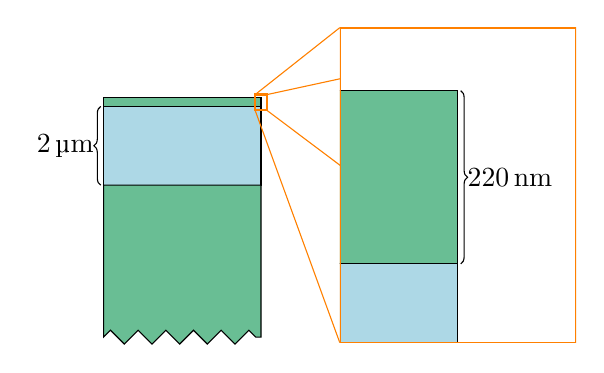
\begin{tikzpicture}
            \begin{scope}[scale=0.05]
                \filldraw[fill=Si_green] (0cm, 0cm) rectangle (40cm, 22mm);
                \filldraw[fill=SiO2_blue] (0cm, -20cm) rectangle (40cm, 0cm);
                \draw[decorate,decoration={brace, raise=1pt}] (0cm, -20cm) -- (0cm, 0mm) node[midway, anchor=east]{\qty{2}{\um}};
                \filldraw[fill=Si_green] (0cm, -58.6cm) decorate [decoration=zigzag] {-- (40cm, -58.6cm)} -- (40cm, -20cm) -- (0cm, -20cm) --cycle;
                \draw[orange, thick] (38.5cm, -1cm) rectangle (41.5cm, 3cm);
            \end{scope}
                \begin{scope}
                    \clip (1.9cm, -3cm) rectangle (3cm, 1cm);
                    \draw[orange] (1.925cm, 0.15cm) -- (3cm, 1cm);
                    \draw[orange] (2.075cm, 0.15cm) -- (6cm, 1cm);
                    \draw[orange] (2.075cm, -0.05) -- (6cm, -3cm);
                    \draw[orange] (1.925cm, -0.05) -- (3cm, -3cm);
                \end{scope}
            \begin{scope}[xshift=0.5cm, yshift=-2cm]
                \clip (2.5cm, -1cm) rectangle (5.5cm, 3cm);
                \filldraw[fill=Si_green] (0cm, 0cm) rectangle (4cm, 22mm);
                \draw[decorate,decoration={brace, mirror, raise=1pt}] (4cm, 0cm) -- (4cm, 22mm) node[midway, anchor=west]{\qty{220}{\nm}};
                \filldraw[fill=SiO2_blue] (0cm, -20cm) -- (4cm, -20cm) -- (4cm, 0cm) -- (0mm,0mm) -- cycle;
                \draw[orange, thick] (2.5cm, -1cm) rectangle (5.5cm, 3cm);
            \end{scope}
        \end{tikzpicture}
    }
    \subcaptionbox{\label{110}}{
        \tikzsetnextfilename{110}
        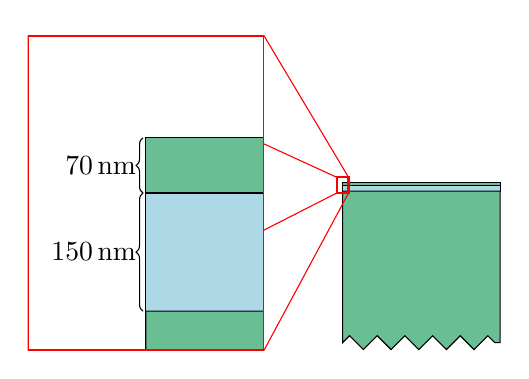
\begin{tikzpicture}
            \begin{scope}[scale=0.05]
                \filldraw[fill=Si_green] (0cm, 0cm) rectangle (40cm, 7mm);
                \filldraw[fill=SiO2_blue] (0cm, -15mm) rectangle (40cm, 0cm);
                \filldraw[fill=Si_green] (0cm, -40cm) decorate [decoration=zigzag] {-- (40cm, -40cm)} -- (40cm, -15mm) -- (0cm, -15mm) --cycle;
                \draw[red, thick] (-1.5cm,-2cm) rectangle (1.5cm,2cm);
            \end{scope}
            \begin{scope}
                \clip (-1cm, -2.1cm) rectangle (1mm, 2cm);
                \draw[red] (-0.075cm, 1mm) -- (-4cm, 1.9cm);
                \draw[red] (0.075cm, 1mm) -- (-1cm, 1.9cm);
                \draw[red] (0.075cm, -1mm) -- (-1cm, -2.1cm);
                \draw[red] (-0.075cm, -1mm) -- (-4cm, -2.1cm);
            \end{scope}
            \begin{scope}[xshift=-2.5cm, yshift=-0.1cm]
                \clip (-1.5cm, -2cm) rectangle (1.5cm, 2cm);
                \filldraw[fill=Si_green] (0cm, 0cm) rectangle (4cm, 7mm);
                \draw[decorate,decoration={brace, raise=1pt}] (0cm, 0cm) -- (0cm, 7mm) node[midway, anchor=east]{\qty{70}{\nm}};
                \draw[decorate,decoration={brace, raise=1pt}] (0cm, -15mm) -- (0cm, 0mm) node[midway, anchor=east]{\qty{150}{\nm}};
                \filldraw[fill=SiO2_blue] (0cm, -15mm) rectangle (4cm, 0cm);
                \filldraw[fill=Si_green] (0cm, -3cm) decorate [decoration=zigzag] {-- (4cm, -3cm)} -- (4cm, -15mm) -- (0cm, -15mm) --cycle;
                \draw[red, thick] (-1.5cm, -2cm) rectangle (1.5cm, 2cm);
            \end{scope}

        \end{tikzpicture}
    }
    \caption[Drawing of the layer stack of the two \acs{soi} wafers showing different layer thicknesses.]{Drawing of the layer stack of the two \acs{soi} wafers showing different layer thicknesses, \acs{si} is represented in green and \acs{sio2} in light blue. The cross-section of the \hkl<0 0 1> wafer is shown in \subref{001} with a magnified insert showing the \qty{220}{\nm} - thick \acs{si} device layer. The layer thicknesses in \subref{110} are proportional to the ones in \subref{001} highlighting how thin the \acs{sio2} (\qty{150}{\nm}) and \acs{si} (\qty{70}{\nm}) layers are in comparison.}
    \label{fig:wafer_thicknesses}
\end{figure}

The tool responsible carried out the dicing cuts at a wafer dicing machine. Every dice is designed to be further divided into nine identical \qtyproduct{2 x 2}{cm} smaller dice that, in turn, contain the \acs{ebl} write regions. This means that every large dice produces nine smaller sample dice that all include the same nanostructure designs but can be grown separately: this considers the possibility of error or damage to some of the smaller dice during processing. The first wafer was cut in \qtyproduct{6.5 x 6.5}{cm} dice for ease of handling at the \acs{ebl} machine. However, it was found that this presented issues with other tools at later steps. Therefore the dice dimensions were reduced to \qtyproduct{6 x 6}{cm} for the second wafer. Figures \ref{fig:markers}, \ref{fig:litho1}, and \ref{fig:litho2} show schematic drawings of the primary process steps as they appear when applied to the \hkl<1 1 0> wafer, but the process steps are the same on the \hkl<0 0 1> wafer.
 \par 
The device layer defines the shape of the \acl{si} seeds and III-V nanostructures. To do so, two lithography steps are needed, one defining the geometry of the wires and one opening the template oxide that encases them. The alignment between these two steps is critical. Much like the definition of the nanostructures themselves, it requires an accuracy of the order of the nanometre on a dice size of \qty{2}{cm}. This resolution is only available with \acf{ebl} lithography in a research environment. A third \acs{ebl} lithography step is introduced to ensure correct alignment. Markers that the \acs{ebl} machine will use to determine the position of the sample with the necessary accuracy are defined in this process step. While I created the mask designs and provided the substrate ready for exposure, given its high degree of complexity, automation, and workload, the machine was loaded and operated by the tool responsible.
\par
The creation of the alignment markers constitutes an important pre-processing step. A \qty{10}{nm} thick \acs{sio2} protective layer is deposited on top of the device layer using \acf{pecvd} before sputtering a \qty{100}{\nm} \acf{w} layer on top of the wafer (figure \ref{W_deposition}). The sputtering tool was operated by the responsible for the tool. \Acl{w} is used to achieve high contrast in the electron microscopy image that the \acs{ebl} machine uses to orient itself on the sample. A negative photoresist is spun before submitting the wafer for the first \acs{ebl} run. During this step, the \acs{ebl} markers are defined in the resist, which, after development, acts as a mask that protects only certain areas of the \acl{w} layer. \Acf{rie} is used to remove the unprotected \acl{w}: this leaves well-defined markers on the wafer (figure \ref{W_markers}).  

\begin{figure}
    \centering
    \subcaptionbox{Sputtered \acs{w}.\label{W_deposition}}{
        \tikzsetnextfilename{W_deposition}
    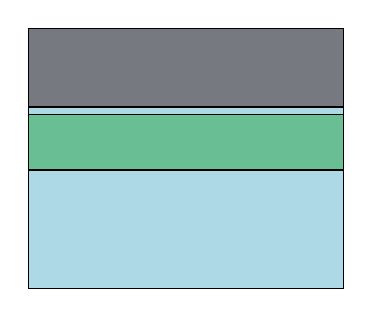
\begin{tikzpicture}
        \filldraw[fill=W_gray] (0cm, 8mm) rectangle (4cm, 1.8cm);
        \filldraw[fill=SiO2_blue] (0cm, 7mm) rectangle (4cm, 8mm);
        \filldraw[fill=Si_green] (0cm, 0cm) rectangle (4cm, 7mm);
        \filldraw[fill=SiO2_blue] (0cm, -15mm) rectangle (4cm, 0cm);
    \end{tikzpicture}
    }
    \subcaptionbox{\acs{w} markers.\label{W_markers}}{
        \tikzsetnextfilename{W_markers}
    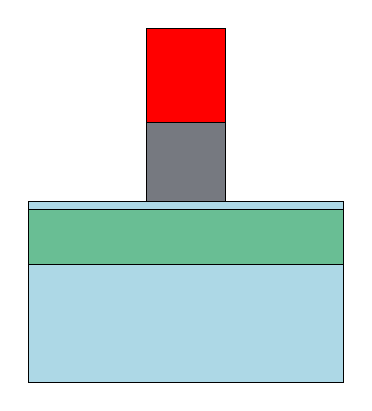
\begin{tikzpicture}
        \filldraw[fill=red] (1.5cm, 1.8) rectangle (2.5cm, 3cm);
        \filldraw[fill=W_gray] (1.5cm, 8mm) rectangle (2.5cm, 1.8cm);
        \filldraw[fill=SiO2_blue] (0cm, 7mm) rectangle (4cm, 8mm);
        \filldraw[fill=Si_green] (0cm, 0cm) rectangle (4cm, 7mm);
        \filldraw[fill=SiO2_blue] (0cm, -15mm) rectangle (4cm, 0cm);
    \end{tikzpicture}
    }
    \subcaptionbox{\acs{w} markers encased in a \acs{sio2} layer.\label{marker_protection_layer}}{
        \tikzsetnextfilename{marker_protection_layer}
    \begin{tikzpicture} [scale=0.5]
        \filldraw[fill=SiO2_blue] (-5cm, 0.7cm) -- (1.5cm, 0.7cm) -- (9cm, 0.7cm)  -- (9cm, 3.7cm) -- (5.5cm, 3.7cm) -- (5.5cm, 4.8cm) -- (-1.5cm, 4.8cm) -- (-1.5cm, 3.7cm) -- (-5cm, 3.7cm) -- cycle;
        \filldraw[fill=W_gray] (1.5cm, 8mm) rectangle (2.5cm, 1.8cm);
        \filldraw[fill=SiO2_blue] (1.5cm, 7mm) rectangle (2.5cm, 8mm);
        \filldraw[fill=Si_green] (-5cm, 0cm) rectangle (9cm, 7mm);
        \filldraw[fill=SiO2_blue] (-5cm, -15mm) rectangle (9cm, 0cm);
    \end{tikzpicture}
    } 
    \subcaptionbox{Definition of the marker protection area.\label{mp_optolitho}}{
        \tikzsetnextfilename{mp_optolitho}
    \begin{tikzpicture} [scale=0.5]
        \filldraw[fill=red] (-1.5cm, 4.7cm) rectangle (5.5cm, 5.7cm);
        \filldraw[fill=SiO2_blue] (-5cm, 0.7cm) -- (1.5cm, 0.7cm) -- (9cm, 0.7cm)  -- (9cm, 3.7cm) -- (5.5cm, 3.7cm) -- (5.5cm, 4.8cm) -- (-1.5cm, 4.8cm) -- (-1.5cm, 3.7cm) -- (-5cm, 3.7cm) -- cycle;
        \filldraw[fill=W_gray] (1.5cm, 8mm) rectangle (2.5cm, 1.8cm);
        \filldraw[fill=Si_green] (-5cm, 0cm) rectangle (9cm, 7mm);
        \filldraw[fill=SiO2_blue] (-5cm, -15mm) rectangle (9cm, 0cm);
    \end{tikzpicture}
    }
    \subcaptionbox{The excess \acs{sio2} is etched away. \label{mp_completed}}{
        \tikzsetnextfilename{mp_completed}
    \begin{tikzpicture} [scale=0.5]
        \filldraw[fill=SiO2_blue] (-1.5cm, 0.7cm) -- (5.5cm, 0.7cm) -- (5.5cm, 3.7cm) -- (5.5cm, 4.8cm) -- (-1.5cm, 4.8cm) -- (-1.5cm, 3.7cm) -- cycle;
        \filldraw[fill=W_gray] (1.5cm, 8mm) rectangle (2.5cm, 1.8cm);
        \filldraw[fill=Si_green] (-5cm, 0cm) rectangle (9cm, 7mm);
        \filldraw[fill=SiO2_blue] (-5cm, -15mm) rectangle (9cm, 0cm);
    \end{tikzpicture}
    }
    \caption[Drawings showing the fabrication process of the \acs{w} markers and marker protection.]{Drawings showing the fabrication process of the \acs{w} markers and marker protection. The sputtered \acs{w} layer \subref{W_deposition} is first patterned \subref{W_markers} and then encased in \qty{300}{\nm}-thick \acs{sio2} layer \subref{marker_protection_layer}. The marker protection area is defined through optical lithography \subref{mp_optolitho}, and then the excess \acs{sio2} is removed \subref{mp_completed}.}
    \label{fig:markers}
\end{figure}

\par
The alignment markers are then protected from the next aggressive etching steps that follow in the \acs{tase} process by depositing a \qty{300}{\nm} thick \acl{sio2} layer on the entire wafer with \acs{pecvd}. This protective layer is then annealed at \qty{750}{\degreeCelsius} for \qty{300}{s} to improve its resistance to etching (Figure \ref{marker_protection_layer}). This cover shields both the alignment markers and the device layer. However, the device layer must be accessible to define the nanostructures that will form the base of the \acs{tase} process. Optical lithography is used to pattern openings in a positive optical resist, leaving only the areas of the \acs{sio2} film above the \acl{w} markers masked (Figure \ref{mp_optolitho}). After development, the \acl{sio2} layer can be removed in correspondence with these openings using a diluted \acf{hf} solution (figure \ref{mp_completed}), uncovering most of the device \acs{si} layer. Reflectometry can ascertain the presence and thickness of the device \acs{si} layer, thereby evaluating the health of the wafer after the pre-processing steps.
\par
This concludes the initial steps that prepare the wafer to go through the \acs{tase} process. In the following illustrations (figures \ref{fig:litho1} and \ref{fig:litho2}), the \acl{w} markers and their oxide protection are omitted as they will not be affected by the following process steps in a process-relevant manner. Still, they are not removed and are the basis for alignment in the next lithography steps.


\section{Nanostructure definition and template deposition}
\label{sec:nanostructure-def_template-dep}
\begin{figure}
    \centering
    \subcaptionbox{\acs{hsq} layer on top of the wafer after exposure.\label{L1_exposed_resist}}{
        \tikzsetnextfilename{L1_exposed_resist}
    \begin{tikzpicture}
        \filldraw[fill=red] (0cm, 7mm) rectangle (10cm, 10mm);
        \filldraw[fill=SiO2_blue] (3cm, 7mm) rectangle (7cm, 10mm);
        \filldraw[fill=Si_green] (0cm, 0cm) rectangle (10cm, 7mm);
        \filldraw[fill=SiO2_blue] (0cm, -15mm) rectangle (10cm, 0cm);
    \end{tikzpicture}
    }
    \subcaptionbox{Nanostructure geometry transferred onto the \acs{si} device layer.\label{L1_nanostructure}}{
        \tikzsetnextfilename{L1_nanostructure}
    \begin{tikzpicture}
        \filldraw[fill=SiO2_blue] (3cm, 7mm) rectangle (7cm, 9mm);
        \filldraw[fill=Si_green] (3cm, 0cm) rectangle (7cm, 7mm);
        \filldraw[fill=SiO2_blue] (0cm, -15mm) rectangle (10cm, 0cm);
    \end{tikzpicture}
    }
    \subcaptionbox{\acs{si} nanostructures encased in the template oxide.\label{L1_template}}{
        \tikzsetnextfilename{L1_template}
    \begin{tikzpicture}
        \filldraw[fill=SiO2_blue] (0cm, 0mm) -- (10cm, 0mm) -- (10cm, 10mm) -- (8cm, 10mm) -- (8cm, 17mm) -- (7cm, 17mm) -- (7cm, 19mm) -- (3cm, 19mm) -- (3cm, 17mm) -- (2cm, 17mm) -- (2cm, 10mm) -- (0cm, 10mm) -- cycle;
        \filldraw[fill=Si_green] (3cm, 0cm) rectangle (7cm, 7mm);
        \filldraw[fill=SiO2_blue] (0cm, -15mm) rectangle (10cm, 0cm);
    \end{tikzpicture}
    }
    \caption[Drawings showing the fabrication process of the silicon nanostructures and \acs{tase} template.]{Drawings showing \subref{L1_exposed_resist} the \acs{hsq} layer after exposure (red unexposed, blue exposed), \subref{L1_nanostructure} the nanostructures as defined in the device \acs{si} layer, and \subref{L1_template} the nanostructures encased in the template oxide.}
    \label{fig:litho1}
\end{figure}

The first step of the \acs{tase} process is to define the geometry of the seed and the nanostructure. An \acs{ebl} mask is designed using mask design software, such as L-Edit, and has to be then transferred onto the device \acs{si} layer: practically, this is accomplished using \acf{hsq} as a resist. This negative \acs{ebl} resist allows for very high-precision pattern transfer through \acs{ebl} lithography. After development, \acs{hsq} leaves a thin layer of \acl{sio2} covering the area corresponding to the nanostructures that will be fabricated (figure \ref{L1_exposed_resist}). The unprotected device layer \acl{si} is removed using \ce{HBr}-based \acf{icp} etching. The resulting \acl{si} nanostructures reflect the geometry of both the \acl{si} seed and the III-V wire that will be grown (Figure \ref{L1_nanostructure}). 
\par
The template \acl{sio2} is then deposited and encases the \acl{si} nanostructures as illustrated in figure \ref{L1_template}. The template deposition step is particularly delicate as the template oxide must closely follow the geometry of the \acl{si} nanostructures. \Acf{ald} enables this level of precision. With this method, the template oxide grows in steps: first, a complete layer of oxygen atoms is deposited, followed by an entire layer of \acl{si} atoms, and so on. Although time-consuming, this growth allows the template oxide to closely follow the geometry of the silicon nanostructures and grow in an ordered manner, resulting in strong etch resistance. 



\section{Etch-back and growth}
\label{etch_growth}
\begin{figure}
    \centering
    \subcaptionbox{Openings patterned on a positive resist layer.
    \label{L2_resist}}{
        \tikzsetnextfilename{L2_resist}
        \begin{tikzpicture}
            \filldraw[fill=red] (0cm, 10mm) -- (7cm, 10mm) -- (7cm, 27mm) -- (0cm, 27mm) -- cycle;
            \filldraw[fill=red] (9cm, 10mm) -- (10cm, 10mm) -- (10cm, 27mm) -- (9cm, 27mm) -- cycle;
            \filldraw[fill=SiO2_blue] (0cm, 0mm) -- (10cm, 0mm) -- (10cm, 10mm) -- (9cm, 10mm) -- (9cm, 17mm) -- (8cm, 17mm) -- (8cm, 19mm) -- (2cm, 19mm) -- (2cm, 17mm) -- (1cm, 17mm) -- (1cm, 10mm) -- (0cm, 10mm) -- cycle;
            \filldraw[fill=Si_green] (2cm, 0cm) rectangle (8cm, 7mm);
            \filldraw[fill=SiO2_blue] (0cm, -14mm) rectangle (10cm, 0cm);
        \end{tikzpicture}
    }
    \subcaptionbox{Etch down of the template \acs{sio2} and device \acs{si} to reach the buried oxide layer.
    \label{L2_open}}{
        \tikzsetnextfilename{L2_open}
        \begin{tikzpicture}
            \filldraw[fill=SiO2_blue] (0cm, 0mm) -- (7cm, 0mm) -- (7cm, 19mm) -- (2cm, 19mm) -- (2cm, 17mm) -- (1cm, 17mm) -- (1cm, 10mm) -- (0cm, 10mm) -- cycle;
            \filldraw[fill=SiO2_blue] (9cm, 0mm) -- (10cm, 0mm) -- (10cm, 10mm) -- (9cm, 10mm) -- cycle;
            \filldraw[fill=Si_green] (2cm, 0cm) rectangle (7cm, 7mm);
            \filldraw[fill=SiO2_blue] (0cm, -14mm) rectangle (10cm, 0cm);
        \end{tikzpicture}
    }
    \subcaptionbox{Etch back of the \acs{si} to create the seed.
    \label{L2_etchback}}{
        \tikzsetnextfilename{L2_etchback}
        \begin{tikzpicture}
            \filldraw[fill=SiO2_blue] (0cm, 0mm) -- (2cm, 0mm)-- (2cm, 7mm) -- (7cm, 7mm) -- (7cm, 19mm) -- (2cm, 19mm) -- (2cm, 17mm) -- (1cm, 17mm) -- (1cm, 10mm) -- (0cm, 10mm) -- cycle;
            \filldraw[fill=SiO2_blue] (9cm, 0mm) -- (10cm, 0mm) -- (10cm, 10mm) -- (9cm, 10mm) -- cycle;
            \filldraw[fill=Si_green] (2cm, 0cm) -- (2cm, 7mm) -- (3.5cm, 7mm) -- (3.5cm, 0mm) -- cycle;
            \filldraw[fill=SiO2_blue] (0cm, -14mm) rectangle (10cm, 0cm);
        \end{tikzpicture}
    }
    \subcaptionbox{A III-V crystal (orange) was grown from the \acs{si} seed.
    \label{L2_growth}}{
        \tikzsetnextfilename{L2_growth}
        \begin{tikzpicture}
            \filldraw[fill=orange] (3.5cm, 7mm) -- (3.5cm, 0mm) -- (6cm, 0mm) -- (6cm, 7mm) -- cycle;
            \filldraw[fill=SiO2_blue] (0cm, 0mm) -- (2cm, 0mm)-- (2cm, 7mm) -- (7cm, 7mm) -- (7cm, 19mm) -- (2cm, 19mm) -- (2cm, 17mm) -- (1cm, 17mm) -- (1cm, 10mm) -- (0cm, 10mm) -- cycle;
            \filldraw[fill=SiO2_blue] (9cm, 0mm) -- (10cm, 0mm) -- (10cm, 10mm) -- (9cm, 10mm) -- cycle;
            \filldraw[fill=Si_green] (2cm, 0cm) -- (2cm, 7mm) -- (3.5cm, 7mm) -- (3.5cm, 0mm) -- cycle;
            \filldraw[fill=SiO2_blue] (0cm, -14mm) rectangle (10cm, 0cm);
        \end{tikzpicture}
    }
    \caption[Drawings showing the last steps of the \acs{tase} process.]{Drawings showing the last steps of the \acs{tase} process. A positive resist layer is patterned \subref{L2_resist} and used as a mask for the \acs{rie} etch-down of holes in the template \acs{sio2}, exposing a vertical and flat \acs{si} surface \subref{L2_open}. \acs{tmah} etch-back \subref{L2_etchback} and \acs{mocvd} growth follow, creating a III-V nanostructure (orange) in the place previously occupied by \acs{si} \subref{L2_growth}.}
    \label{fig:litho2}
\end{figure}

The last lithography step involves defining the opening areas in the template oxide through which the etch back and growth occur. Holes are defined in a positive resist layer (Figure \ref{L2_resist}). After \acs{ebl} exposure and development, \acs{rie} is used to etch the template oxide and the device \acl{si} underneath through these holes, with good vertical selectivity (Figure \ref{L2_open}). After opening the template, each \qtyproduct{6.5 x 6.5}{\cm} or \qtyproduct{6 x 6}{\cm} dice is further cut into smaller \qtyproduct{2 x 2}{cm} dice that will then be etched back and grown singularly as described in the following paragraphs.
\par
Excess \acl{si} to be substituted with III-V material is removed using a \qty{2.5}{\%_{V\per\V}} \acf{tmah}/\ce{H2O} solution heated at \qty{80}{\degreeCelsius}. This solution has a reliable etch-back speed of \qty{60}{\nm\per\minute}.  The etch back proceeds from the template openings to leave only the seed area inside an empty \acl{sio2} template where the III-V crystal will grow (Figure \ref{L2_etchback}). \Acs{tmah} is specifically chosen because it has good selectivity to \acs{si}, therefore leaving the \acs{sio2} template mostly unaffected. A small amount of template etching still takes place and must be considered when etching multiple micrometres of \acs{si} by depositing a thicker template oxide in previous fabrication steps. Another advantage of \acs{tmah} etching is that it results in \acl{si} seeds terminated by \hkl{1 1 1} facets that avoid antiphase boundary formation during \acf{mocvd} \cite{Kunert2018}. After etching, the chip is ready for III-V material growth, pre-growth surface treatment steps include a dip in a 2:1 \acf{h2so4} / \acf{h2o2} solution to remove organic contaminants and a further \qty{10}{s} dip in a diluted \acs{hf} solution to remove the native oxide layer. 
\par
Before growth and in the chamber, the chip is also thermally treated at \qty{780}{\degreeCelsius} for \qty{3}{\minute} in an \acs{as} atmosphere to facilitate oxygen desorption from the \acs{si} seed. The nucleation of the III-V material is selective to the \acl{si} seeds. This means that the growth of the III-V nanostructures is limited to the areas defined in the previous lithography steps (Figure \ref{L2_growth}). At the beginning of this project, the DESIGN-EID consortium chose the \acf{ingaas} / \acf{inp} material system, and these are the III-V semiconductors that I grew in the templates using \acs{mocvd}.
%\chapter{Fabrication and Characterization Tools}
\label{chap:tools}

The \acf{brnc} is a facility at \acs{ibm} Research Europe – Zurich, in Rueschlikon, Zurich, Switzerland. It consists of a cleanroom and Noise-free lab. All the experimental work on the growth and characterisation of nanostructures presented in this work took place at \acs{ibm} Research Europe - Zurich, most of it within the \acs{brnc} itself. 

\section{Cleanroom Tools}

The \acs{brnc} cleanroom is a \qty{950}{\m^2} area with different rooms ranging in cleanroom classification from 100 (ISO 5) to 10’000 (ISO 7). Most of the chemicals and tools used during the \acf{tase} process and sample preparation are within these rooms. 
\par
The following tools, located in the \acs{brnc} cleanroom, were used:
\begin{itemize}
    \item wet benches, as fume hoods are impractical in a cleanroom: while in fume hoods, the vapours and gasses are aspirated upwards, on the wet benches they are evacuated through the work surface, thanks to holes in it and an applied negative pressure gradient under it. These workstations have smaller tools, such as spin coaters for resist application, hot plates, and ultrasound baths. Solution-based etching can also be carried out on wet benches safely with different dangerous chemicals such as strong acids and bases and toxic reagents,
    \item \acf{pecvd} tool: Oxford Plasma Pro 100 for \acl{sio2} deposition,
    \item \acf{ald} tool: Oxford FlexAL,
    \item \acf{rie} tool: Oxford Plasma Pro NPG 80, which employs a chemically active plasma to etch oxides or metal,
    \item \acf{icp} etching tool: Oxford Plasmalab System 100. This tool employs a chemically active inductively coupled plasma to achieve extremely anisotropic etching of \acl{si},
    \item mask aligner: Seuss Mask Aligner MA6 to execute photolithography steps with pre-written metal masks,
    \item rapid thermal annealer Annealsys AS-one 150 for high-temperature annealing treatments of deposited material layers,
    \item dual beam \acf{fib} tool: FEI Helios NanoLab 450S, for SEM imaging; and lamella cutting, manipulation, and thinning,
    \item plasma cleaner PVA TePla Plasma Asher for the removal of resist traces and surface preparation,
    \item reflectometer: Nanospec II 150-VIS to measure the thickness of deposited material layers,
    \item multiple optical microscopes to monitor the fabrication process,
    \item Raman spectroscope: ND-MDT NTEGRA Spectra.
\end{itemize}
 
\section{Noise-Free Labs Tools}

The \acs{brnc} Noise-free labs consist of \qty{176}{\m^2} of noise-shielded laboratory area. The shielding limits vibration noise to \qty{300}{\nm\per\s} at \qty{1}{Hz}, and to \qty{10}{\nm\per\s} at frequencies higher than \qty{100}{Hz}; temperature fluctuations to \qty{0.01}{\degreeCelsius}; humidity variations to \qty{2}{\%}; acoustic noise level to \qty{21}{dBc}; and electromagnetic noise to \qty{0.3}{\nano\tesla} AC, and to \qty{15}{\nano\tesla} DC \cite{Lörtscher_Noise_Free}. These technical specifications are instrumental in successfully recording atomic-resolution \acf{stem_m} images, making the laboratory rooms a tool in their own right.
\par
Two of the tools in the Noise-free labs were used in this work, relating to the \acs{stem_m} measurements I carried out. The first is the plasma cleaner Fischione Model 1020 for the final oxygen-argon plasma cleaning (effective in removing hydrocarbon contamination) of the lamella before insertion in the \acs{stem_i}. 
\par 
The \acl{stem_i} JEOL ARM200F is the second tool. This microscope is equipped with a cold field emission gun placed in a \qty{200}{\kV} extraction and acceleration potential drop (emitting with an energy width of less than \qty{0,3}{eV}), hexapole optics, \acf{bf}, \acf{adf}, and \acf{haadf} detectors. Two spectroscopic techniques are also available on this microscope in the form of \acf{eds} and \acf{eels}. The \acs{eds} tool JED-2300T was used to characterise the samples. This tool is equipped with a \qty{100}{\mm^2} detector surface that allows for very fast \acs{eds} mapping. The detector is equipped with an ultra-thin window, which provides excellent performance for analysing light elements. Resolution for the Mn K$\alpha$ line is less than \qty{138}{\eV}. \qty{1}{\steradian} collection solid angle. This tool can also be operated as a \acf{tem_i}.

\section{Other Tools}

Outside both the cleanroom and Noise-free lab, the following tools were instrumental in achieving the experimental results:
\begin{itemize}
    \item \acf{sem_i}: Hitachi SU8000 type II to monitor the fabrication process,
    \item a “home-built” \acf{mocvd} setup in which the III-V nanowires were grown. The vertical reactor contains a showerhead, which introduces precursors in the chamber. The rotating susceptor can accommodate three 2-inch wafers, or smaller pieces, such as the \qtyproduct{2 x 2}{\cm} dices used in this work, utilising carriers \cite{Brugnolotto2023}.
\end{itemize}
\par
The precursors used in the growth of III-V material are:
\begin{itemize}
    \item \acf{tmin},
    \item \acf{tmga},
    \item \acf{tbas},
    \item \acf{tbp},
    \item \acf{tmsb},
    \item \acf{tesn} (as a dopant)
\end{itemize}

The \acf{gms} software was used to record and later analyse the microscopy images and \acs{eds} data. L-Edit and KLayout were used to design and visualise the \acf{ebl} and optical lithography masks in GDSII format. 
\par 
Tools that I did not operate personally but were used in the fabrication or characterisation of my samples were:
\begin{itemize}
    \item sputter tool: Von Ardenne CS 320S to deposit the tungsten that makes up the \acl{ebl} markers,
    \item \acl{ebl} tool Vistec EBPG 5200+ for exposure of electron-sensitive resists,
    \item laser writer: Heidelberg DWL 2000 for the creation of optical lithography masks (glass substrate, metallic layer mask),
    \item dicer tool: ADT ProVectus LA 7100 for dicing large wafers into smaller dices,
    \item a “home-built” photoluminescence spectroscope for photoluminescence characterisation.
\end{itemize}

\backmatter  % Turn off chapter numbering

\printbibliography

\end{document}
